% arara: pdflatex
% arara: makeindex: {style: latexindent.ist}
% arara: bibtex
% arara: pdflatex if changed (toFile('latexindent.aux')) || changed (toFile('latexindent.ind')) 
% arara: pdflatex if changed (toFile('latexindent.aux')) 
% arara: pdflatex if changed (toFile('latexindent.aux')) 
\documentclass[10pt]{article}
%   This program is free software: you can redistribute it and/or modify
%   it under the terms of the GNU General Public License as published by
%   the Free Software Foundation, either version 3 of the License, or
%   (at your option) any later version.
%
%   This program is distributed in the hope that it will be useful,
%   but WITHOUT ANY WARRANTY; without even the implied warranty of
%   MERCHANTABILITY or FITNESS FOR A PARTICULAR PURPOSE. See the
%   GNU General Public License for more details.
%
%   See <http://www.gnu.org/licenses/>.
\usepackage[left=4.5cm,right=2.5cm,showframe=false,
 top=2cm,bottom=1.5cm,marginparsep=2cm]{geometry} % page setup
\usepackage{lmodern}
\usepackage{parskip}                                 % paragraph skips
\usepackage{booktabs}                                % beautiful tables
\usepackage{listings}                                % nice verbatim environments
\usepackage{titlesec}                                % customize headings
\usepackage{titletoc}                                % customize headings
\usepackage{multicol}
\usepackage{changepage}                              % adjust width of page
\usepackage{fancyhdr}                                % headers & footers
\usepackage{fontawesome}
\usepackage[sc,format=hang,font=small]{caption}      % captions
\usepackage[backend=bibtex,sorting=ynt]{biblatex}    % bibliography
\usepackage{tcolorbox}                               % framed environments
\usepackage{tikz}
\usepackage{xparse}
\usepackage[charter]{mathdesign}                     % changes font
\usepackage[expansion=false,kerning=true]{microtype} % better kerning
\usepackage{enumitem}                                % custom lists
\usepackage{longtable}
\usepackage{array}
\usepackage{totalcount}
\usepackage{standalone}
% setup gitinfo2, as in the manual, details just above begin{document}
\usepackage[mark]{gitinfo2}
% tikz, tcolorbox libraries
\usetikzlibrary{positioning}
\usetikzlibrary{decorations.pathmorphing}
\usetikzlibrary{decorations,shapes}
\usepackage{varioref}                                % the documentation library from tcolorbox loads hyperref
\tcbuselibrary{breakable,xparse,documentation,hooks,raster}
\hypersetup{
 pdfauthor={Chris Hughes},
 pdftitle={latexindent.pl package},
 pdfkeywords={perl;beautify;indentation},
 bookmarksnumbered,
 bookmarksopen,
 linktocpage,
 colorlinks=true,
 linkcolor=blue,
 citecolor=black,
}
\usepackage{cleveref}

% create my own star style, for re-use at various points
\tikzset{cmhstar/.style={star,star point ratio=2.25,fill=cmhgold,draw=orange,}}

% shortcut command for displaying star in documentation
\newcommand{\stardemo}[1][]{\begin{tikzpicture}
 \node at (10:.1cm)[very thin,cmhstar,scale=0.25,rotate=20,#1]{};
 \node at (120:.1cm)[very thin,cmhstar,scale=0.15,rotate=-10,#1]{};
 \node at (235:.1cm)[very thin,cmhstar,scale=0.2,rotate=-20,#1]{};
 \end{tikzpicture}}

% totalcount
\DeclareTotalCounter{lstlisting}

% customise the \tcbdocnew command
\tcbset{doclang/new={{\bfseries\color{green!50!black}N\normalfont\color{black}}}}
\tcbset{doclang/updated={{\bfseries\color{green!50!black}U\normalfont\color{black}}}}
\tcbset{doc marginnote={width=1.6cm}}

% \announce * { YYYY-MM-DD }*{ <announcement text> }
%
%   NEW as of current version
%       \announce*{date}*[text] means *updated* as of <date>
%       \announce*{date}[text]  means *new* as of <date>
%
%   NOT new as of current version
%       \announce{date}*[text] means *updated* as of <date>
%       \announce{date}[text]  means *new* as of <date>
%
\NewDocumentCommand{\announce}{ s m s m }{%
 \IfBooleanTF{#1}%
 {% \announce*
  % NEW in current version
  \tcbdocmarginnote[colframe=orange,
   overlay={\node at ([yshift=0mm,xshift=1mm]frame.north east) {\stardemo}; }]{%
   \IfBooleanTF{#3}%
   {% \announce*{date}*[text] means *updated* as of <date>
    \tcbdocupdated{#2}%
   }%
   {% \announce*{date}[text] means *new* as of <date>
    \tcbdocnew{#2}%
   }%
  }%
  \IfBooleanTF{#3}%
  {%
   \addcontentsline{new}{cmhtitle}{#4 (U)}%
  }%
  {%
   \addcontentsline{new}{cmhtitle}{#4 (N)}%
  }%
 }%
 {% \announce
  % NOT new in current version
  \tcbdocmarginnote[colframe=gray!50!white,
   doclang/new={{\color{gray}N\normalfont\color{gray}}},
   doclang/updated={{\color{gray}U\normalfont\color{gray}}},
  ]{%
   \IfBooleanTF{#3}%
   {% \announce{date}*[text] means *updated* as of <date>
    \tcbdocupdated{#2}%
   }%
   {% \announce{date}[text] means *new* as of <date>
    \tcbdocnew{#2}%
   }%
  }%
 }}

\reversemarginpar
% bibliographies
\addbibresource{latex-indent}
\addbibresource{contributors}

% http://tex.stackexchange.com/questions/122135/how-to-add-a-png-icon-on-the-right-side-of-a-tcolorbox-title
\newtcolorbox{warning}{parbox=false,
 breakable,
 enhanced,
 arc=0mm,
 colback=red!5,
 colframe=red,
 leftrule=12mm,%
 title={Warning!},
 overlay={\node[anchor=north west,outer sep=2pt] at (frame.north west) {
\includegraphics[width=8mm]{warning}}; }
}

\definecolor{harvestgold}{cmyk}{0.00, 0.05, 0.51, 0.07}  %EDE275
\definecolor{cmhgold}{cmyk}{0,0.178,0.909,0.008}         %FDD017
\colorlet{cmhgray}{gray!30!white}

\makeatletter
\tcbset{
 addtolol/.style={list entry={\kvtcb@title},add to list={lol}{lstlisting}},
 addtololstar/.style={list entry={\kvtcb@title},add to list={lol}{lstlistingstar}},
 cmhlistings/.style={
   colback=blue!5!white,
   colframe=white!25!black,colback=white,
   top=0cm,
   bottom=0cm,
   left=0mm,
   listing only,
   center title,
   listing engine=listings,
   listing options={showtabs=true,tabsize=4,showspaces=true},
   boxrule=0pt,
   toprule=1pt,bottomrule=1pt,
   titlerule=1pt,
   colframe=white!40!black,
   colback=white,
   sharp corners,
   colbacktitle=white!75!black
  },
 tex-TCB/.style={
   listing only,
   listing engine=listings,
   left=0cm,
   boxrule=0pt,
   sharp corners,
   center title,
   colframe=white!40!black,
   colback=white,
   sharp corners,
   colbacktitle=white!75!black,
   toprule=1pt,
   bottomrule=1pt,
   titlerule=1pt,
  },
 yaml-TCB/.style={
   listing only,
   listing engine=listings,
   left=0cm,
   boxrule=0pt,
   sharp corners,
   center title,
   colbacktitle=white!75!blue,
   colframe=white!25!blue,
   colback=white!90!blue,
   toprule=2pt,
   titlerule=2pt,
  },
 MLB-TCB/.style={
   yaml-TCB,
   center title,
   colframe=cmhgold,
   colbacktitle=harvestgold,
   colback=white!60!cmhgold,
   width=0.9\linewidth,
   before=\centering,
   enhanced,
   overlay={\node[anchor=north east,outer sep=2pt,draw=cmhgold,very thick,double,fill=harvestgold,font =\small] at ([yshift=-3mm]frame.north east) {\texttt{-m}}; }
  },
 replace-TCB/.style={
   yaml-TCB,
   center title,
   colbacktitle=white!75!green,
   colframe=white!25!green,
   colback=white!90!green,
   width=0.9\linewidth,
   before=\centering,
   enhanced,
   overlay={\node[anchor=north east,outer sep=2pt,draw=white!25!green,very thick,circle,fill=white!75!green,font =\small] at ([yshift=-3mm]frame.north east) {\texttt{-r}}; }
  },
 yaml-obsolete/.style={
   listing only,
   listing engine=listings,
   left=0cm,
   boxrule=0pt,
   sharp corners,
   center title,
   toprule=2pt,
   titlerule=2pt,
   colframe=white!25!red,
   colbacktitle=white!75!red,
   colback=white!90!red,
  },
 new-to-this-version/.style={
   enhanced,
   overlay app={\node at ([yshift=0mm,xshift=0mm]frame.north east) {\stardemo[scale=1.2]}; },
   addtololstar,
  },
}

\DeclareTCBListing[use counter=lstlisting]{cmhlistings}{s O{} m m}{%
 cmhlistings,
 IfBooleanTF={#1}{new-to-this-version}{addtolol},
 center title,
 title={\color{black}{\scshape Listing \thetcbcounter}: ~#3},label={#4},
 listing engine=listings,
 listing options={#2},
}

\DeclareDocumentEnvironment{cmhtcbraster}{O{}}{\begin{tcbraster}[
  new-to-this-version/.style={
    enhanced,
    overlay app={\node[anchor=south east] at ([yshift=-3mm,xshift=3mm]frame.north east) {\stardemo[scale=1.2]}; },
    addtololstar,
   },
  raster valign=top,raster columns=2,#1]}{\end{tcbraster}}

% \cmhlistingsfromfile
%                   * no star: not new, star: new   #1
%                   [ listing options ]             #2
%                   {<name of listing file>}        #3
%                   [<options for tcolorbox>]       #4
%                   {<title>}                       #5
%                   {<label>}                       #6
%
% for example,
%   \cmhlistingsfromfile*[listing options]... is NEW
%   \cmhlistingsfromfile[listing options]...  is not new
\DeclareTCBInputListing[use counter=lstlisting]{\cmhlistingsfromfile}{s O{} m O{} m m}{%
 cmhlistings,
 listing file={#3},
 listing options={style=tcblatex,showspaces=false,#2},
 title={\color{black}{\scshape Listing \thetcbcounter}: ~#5},label={#6},
 #4,
 IfBooleanTF={#1}{new-to-this-version}{addtolol},
}

\makeatletter
\@tempswafalse
\def\@tempa{draft}
\@for\next:=\@classoptionslist\do
{\ifx\next\@tempa\@tempswatrue\fi}
\if@tempswa % draft option is active
 \RenewDocumentCommand{\cmhlistingsfromfile}{s O{} s m O{} m m}{\captionof{lstlisting}{#6}\label{#7}}
 \renewcommand{\stardemo}[1][]{$\star$}
\fi

% command shell
\newtcblisting{commandshell}{colback=black,colupper=white,colframe=yellow!75!black,
 listing only,listing options={style=tcblatex,language=sh,
   morekeywords={latexindent,pl},
   keywordstyle=\color{blue!35!white}\bfseries,
  },
 listing engine=listings,
 left=0cm,
 every listing line={\textcolor{red}{\small\ttfamily\fontseries{b}\selectfont cmh:$\sim$\$ }}}

% dosprompt
\newtcblisting{dosprompt}{
 colback=black,
 colupper=white,
 colframe=yellow!75!black,
 listing only,
 listing options={
   language=command.com,
   morekeywords={latexindent,pl},
   keywordstyle=\color{blue!35!white}\bfseries,
   basicstyle=\small\color{white}\ttfamily
  },
 listing engine=listings,
 left=0cm,
 every listing line={\textcolor{white}{\small\ttfamily\fontseries{b}\selectfont C:\textbackslash Users\textbackslash cmh$>$}}}

\lstset{%
 basicstyle=\small\ttfamily,language={[LaTeX]TeX},
 numberstyle=\ttfamily%\small,
 breaklines=true,
 keywordstyle=\color{blue},                    % keywords
 commentstyle=\color{purple},    % comments
 tabsize=3,
}%
\DeclareTCBListing[use counter=lstlisting]{yaml}{O{} m O{} m}{
 yaml-TCB,
 listing options={
   style=tcblatex,
   numbers=none,
   numberstyle=\color{red},
   #1,
  },
 title={\color{black}{\scshape Listing \thetcbcounter}: ~#2},label={#4},
 #3,
}

\lstdefinestyle{yaml-LST}{
 style=tcblatex,
 numbers=none,
 numberstyle=\color{red},
}

\lstdefinestyle{demo}{
 numbers=none,
 linewidth=1.25\textwidth,
 columns=fullflexible,
}

\lstdefinestyle{lineNumbersTeX}{
 numbers=left,
 numberstyle=\color{blue},
}

\lstdefinestyle{fileExtensionPreference}{
 style=yaml-LST,
 firstnumber=44,linerange={44-48},
 numbers=left,
}

\lstdefinestyle{logFilePreferences}{
 style=yaml-LST,
 firstnumber=88,linerange={88-102},
 numbers=left,
}

\lstdefinestyle{verbatimEnvironments}{
 style=yaml-LST,
 firstnumber=106,linerange={106-109},
 numbers=left,
}

\lstdefinestyle{verbatimCommands}{
 style=yaml-LST,
 firstnumber=112,linerange={112-114},
 numbers=left,
}

\lstdefinestyle{noIndentBlock}{
 style=yaml-LST,
 firstnumber=119,linerange={119-121},
 numbers=left,
}

\lstdefinestyle{removeTrailingWhitespace}{
 style=yaml-LST,
 firstnumber=150,linerange={150-152},
 numbers=left,
}

\lstdefinestyle{fileContentsEnvironments}{
 style=yaml-LST,
 firstnumber=125,linerange={125-127},
 numbers=left,
}

\lstdefinestyle{lookForPreamble}{
 style=yaml-LST,
 firstnumber=133,linerange={133-137},
 numbers=left,
}

\lstdefinestyle{lookForAlignDelims}{
 style=yaml-LST,
 firstnumber=155,linerange={155-171},
 numbers=left,
}

\lstdefinestyle{indentAfterItems}{
 style=yaml-LST,
 firstnumber=234,linerange={234-241},
 numbers=left,
}

\lstdefinestyle{itemNames}{
 style=yaml-LST,
 firstnumber=247,linerange={247-249},
 numbers=left,
}

\lstdefinestyle{specialBeginEnd}{
 style=yaml-LST,
 firstnumber=253,linerange={253-266},
 numbers=left,
}

\lstdefinestyle{indentAfterHeadings}{
 style=yaml-LST,
 firstnumber=276,linerange={276-285},
 numbers=left,
}

\lstdefinestyle{noAdditionalIndentGlobalEnv}{
 style=yaml-LST,
 firstnumber=334,linerange={334-335},
 numbers=left,
}

\lstdefinestyle{noAdditionalIndentGlobal}{
 style=yaml-LST,
 firstnumber=334,linerange={334-346},
 numbers=left,
}

\lstdefinestyle{indentRulesGlobalEnv}{
 style=yaml-LST,
 firstnumber=350,linerange={350-351},
 numbers=left,
}

\lstdefinestyle{indentRulesGlobal}{
 style=yaml-LST,
 firstnumber=350,linerange={350-362},
 numbers=left,
}

\lstdefinestyle{commandCodeBlocks}{
 style=yaml-LST,
 firstnumber=365,linerange={365-380},
 numbers=left,
}

\lstdefinestyle{modifylinebreaks}{
 style=yaml-LST,
 firstnumber=495,linerange={495-497},
 numbers=left,
}

\lstdefinestyle{textWrapOptions}{
 style=yaml-LST,
 firstnumber=523,linerange={523-524},
 numbers=left,
}

\lstdefinestyle{textWrapOptionsAll}{
 style=yaml-LST,
 firstnumber=523,linerange={523-546},
 numbers=left,
}

\lstdefinestyle{oneSentencePerLine}{
 style=yaml-LST,
 firstnumber=498,linerange={498-522},
 numbers=left,
}

\lstdefinestyle{sentencesFollow}{
 style=yaml-LST,
 firstnumber=504,linerange={504-512},
 numbers=left,
}

\lstdefinestyle{sentencesBeginWith}{
 style=yaml-LST,
 firstnumber=513,linerange={513-516},
 numbers=left,
}

\lstdefinestyle{sentencesEndWith}{
 style=yaml-LST,
 firstnumber=517,linerange={517-522},
 numbers=left,
}

\lstdefinestyle{modifylinebreaksEnv}{
 style=yaml-LST,
 firstnumber=548,linerange={548-557},
 numbers=left,
}

\lstdefinestyle{replacements}{
 style=yaml-LST,
 firstnumber=609,linerange={609-617},
 numbers=left,
}

\lstdefinestyle{fineTuning}{
 style=yaml-LST,
 firstnumber=620,linerange={620-672},
 numbers=left,
}

% stars around contributors
\pgfdeclaredecoration{stars}{initial}{
 \state{initial}[width=15pt]
 {
  \pgfmathparse{round(rnd*100)}
  \pgfsetfillcolor{yellow!\pgfmathresult!orange}
  \pgfsetstrokecolor{yellow!\pgfmathresult!red}
  \pgfnode{star}{center}{}{}{\pgfusepath{stroke,fill}}
 }
 \state{final}
 {
  \pgfpathmoveto{\pgfpointdecoratedpathlast}
 }
}

\newtcolorbox{stars}{%
 enhanced jigsaw,
 breakable, % allow page breaks
 left=0cm,
 top=0cm,
 before skip=0.2cm,
 boxsep=0cm,
 frame style={draw=none,fill=none}, % hide the default frame
 colback=white,
 overlay={
   \draw[inner sep=0,minimum size=rnd*15pt+2pt]
   decorate[decoration={stars,segment length=2cm}] {
     decorate[decoration={zigzag,segment length=2cm,amplitude=0.3cm}] {
       ([xshift=-.5cm,yshift=0.1cm]frame.south west) -- ([xshift=-.5cm,yshift=0.4cm]frame.north west)
      }};
   \draw[inner sep=0,minimum size=rnd*15pt+2pt]
   decorate[decoration={stars,segment length=2cm}] {
     decorate[decoration={zigzag,segment length=2cm,amplitude=0.3cm}] {
       ([xshift=.75cm,yshift=0.1cm]frame.south east) -- ([xshift=.75cm,yshift=0.6cm]frame.north east)
      }};
   \node[anchor=north west,outer sep=2pt,opacity=0.25] at ([xshift=-4.25cm]frame.north west) {\resizebox{3cm}{!}{\faGithub}};
  },
 % paragraph skips obeyed within tcolorbox
 parbox=false,
}

\newtcolorbox[auto counter]{example}{breakable,
 enhanced jigsaw,
 before skip=6pt,after skip=6pt,
 frame hidden,
 title={\llap{Example~\thetcbcounter\hspace{3mm}}},
 fonttitle=\bfseries,
 coltitle=black,
 attach title to upper,
 grow to left by=5mm,
 top=3mm,
 overlay unbroken={%
   \draw[thick,cmhgray] ([xshift=3mm]interior.north east)--([xshift=3mm]interior.south east);
   \path [fill=cmhgray] ([xshift=3mm]interior.north east) circle (.5mm);
   \path [fill=cmhgray] ([xshift=3mm]interior.south east) circle (1mm);
  },
 overlay first={%
   \draw[thick,cmhgray] ([xshift=3mm]interior.north east)--([xshift=3mm]interior.south east);
   \path [fill=cmhgray] ([xshift=3mm]interior.north east) circle (.5mm);
   %\path [draw=cmhgray,fill=white] ([xshift=3mm]interior.south east) circle (.5mm);
  },
 overlay last={%
   \draw[thick,cmhgray] ([xshift=3mm]interior.north east)--([xshift=3mm]interior.south east);
   %\path [fill=white,draw=cmhgray] ([xshift=3mm]interior.north east) circle (.5mm);
   \path [fill=cmhgray] ([xshift=3mm]interior.south east) circle (1mm);
  },
 parbox=false,
}

% copied from /usr/local/texlive/2013/texmf-dist/tex/latex/biblatex/bbx/numeric.bbx
% the only modification is the \stars and \endstars
\defbibenvironment{specialbib}
{\stars\list
 {\printtext[labelnumberwidth]{%
   \printfield{prefixnumber}%
   \printfield{labelnumber}}}
 {\setlength{\labelwidth}{\labelnumberwidth}%
  \setlength{\leftmargin}{\labelwidth}%
  \setlength{\labelsep}{\biblabelsep}%
  \addtolength{\leftmargin}{\labelsep}%
  \setlength{\itemsep}{\bibitemsep}%
  \setlength{\parsep}{\bibparsep}}%
 \renewcommand*{\makelabel}[1]{\hss##1}}
{\endlist\endstars}
{\item}

\newtcbox{yamltitlebox}[1][]{colframe=black!50!white,boxrule=.5pt,sharp corners,#1}

\newcommand{\flagbox}[1]{%
 \par
 \makebox[30pt][l]{%
  \hspace{-1cm}%
  \ttfamily\fontseries{b}\selectfont #1
 }%
}

\NewDocumentCommand{\yamltitle}{O{} m s m}{%
 \par
 \makebox[30pt][l]{%
  \hspace{-2cm}%
  \yamltitlebox[#1]{%
   {\ttfamily\fontseries{b}\selectfont{\color{blue!80!white}#2}}: %
   \IfBooleanTF{#3}
   {$\langle$\itshape #4$\rangle$}
   {{\bfseries #4}}
  }}
 \par\nobreak%
}

\newcommand{\fixthis}[1]
{%
 \marginpar{\huge \color{red} \framebox{FIX}}%
 \typeout{FIXTHIS: p\thepage : #1^^J}%
}

\newcommand*\ruleline[1]{%
 \par\noindent\raisebox{.8ex}{\makebox[\linewidth]{\hrulefill\hspace{1ex}\raisebox{-1.8ex}{#1}\hspace{1ex}\hrulefill}}}

\newcommand{\imagetouse}{logo-bw}

% custom section
\titleformat% Formatting the header
{\section} % command
[block] % shape - Only managed to get it working with block
{\normalfont\bfseries\huge} % format - Change here as needed
{\centering {\scshape Section \thesection}\\} % the section
{0pt} % sep
{\centering \ruleline{\includegraphics{\imagetouse}}\\ % The horizontal rule
 \centering} % And the actual title

% custom subsection
\titleformat{\subsection}
{\normalfont\bfseries}
{\llap{\thesubsection\hskip.5cm}}
{0pt}
{}

% custom subsubsection
\titleformat{\subsubsection}
{\normalfont\bfseries}
{\llap{\thesubsubsection\hskip.5cm}}
{0pt}
{}

% custom paragraph
\titleformat{\paragraph}
{\normalfont\bfseries}
{\llap{\theparagraph\hskip.5cm}}
{0pt}
{}

% title spacing
\titlespacing\section{0pt}{12pt plus 4pt minus 2pt}{34pt plus 2pt minus 2pt}
\titlespacing\subsection{0pt}{12pt plus 4pt minus 2pt}{4pt plus 2pt minus 2pt}
\titlespacing\subsubsection{0pt}{12pt plus 4pt minus 2pt}{4pt plus 2pt minus 2pt}
\titlespacing\paragraph{0pt}{12pt plus 4pt minus 2pt}{4pt plus 2pt minus 2pt}

% list of listings
\contentsuse{lstlisting}{lol}
\titleclass{\lstlistingstar}{straight}[\section]
\titleformat{\lstlistingstar}{}{}{}{}
\titlecontents{lstlistingstar}[2em]
  {\addvspace{0.25pc}}
  {}
  {\llap{\stardemo}\thecontentslabel}
  {\titlerule*[0.5em]{$\cdot$}\contentspage}
  []
\titlecontents{lstlisting}[2em]
  {\addvspace{0.25pc}}
  {\thecontentslabel}
  {\thecontentslabel}
  {\titlerule*[0.5em]{$\cdot$}\contentspage}
  []
\AtBeginDocument{\addtocontents{lol}{\protect\begin{widepage}\protect\begin{multicols}{2}}}
\preto{\printindex}{\addtocontents{lol}{\protect\end{multicols}\protect\end{widepage}}}

% cleveref settings
\crefname{table}{Table}{Tables}
\Crefname{table}{Table}{Tables}
\crefname{figure}{Figure}{Figures}
\Crefname{figure}{Figure}{Figures}
\crefname{section}{Section}{Sections}
\Crefname{section}{Section}{Sections}
\crefname{listing}{Listing}{Listings}
\Crefname{listing}{Listing}{Listings}

% headers and footers
\fancyhf{} % delete current header and footer
\fancyhead[R]{\bfseries\thepage%
 \tikz[remember picture,overlay] {
  \node at (1,0){
\includegraphics{logo-bw}}; }
}
\fancyhead[L]{\rightmark}
\fancyheadoffset[L]{3cm}
\pagestyle{fancy}

% renew plain style
\fancypagestyle{plain}{%
 \fancyhf{} % clear all header and footer fields
 \renewcommand{\headrulewidth}{0pt}
 \renewcommand{\footrulewidth}{0pt}}

% widepage environment
\newenvironment{widepage}{\begin{adjustwidth}{-3cm}{0cm}}{\end{adjustwidth}}

% symbols for the m switch
\newcommand{\BeginStartsOnOwnLine}{\color{red}\spadesuit}
\newcommand{\BodyStartsOnOwnLine}{\color{red}\heartsuit}
\newcommand{\EndStartsOnOwnLine}{\color{red}\diamondsuit}
\newcommand{\EndFinishesWithLineBreak}{\color{red}\clubsuit}
\newcommand{\ElseStartsOnOwnLine}{\color{red}\bigstar}
\newcommand{\ElseFinishesWithLineBreak}{\color{red}\square}
\newcommand{\OrStartsOnOwnLine}{\color{red}\blacktriangle}
\newcommand{\OrFinishesWithLineBreak}{\color{red}\blacktriangledown}
\newcommand{\EqualsStartsOnOwnLine}{\color{red}\bullet}

% table rules
\setlength\heavyrulewidth{0.25ex}
% gitinfo2 settings
\renewcommand{\gitMark}{\gitBranch\,@\,\gitAbbrevHash{}\,\textbullet{}\,\gitAuthorDate\,\textbullet{}\faGithub\,\textbullet{}\gitRel}

% setting up gitinfo2:
%   copy the file post-xxx-sample.txt from http://mirror.ctan.org/macros/latex/contrib/gitinfo2
%   and put it in .git/hooks/post-checkout
% then
%   cd .git/hooks
%   chmod g+x post-checkout
%   chmod +x post-checkout
%   cp post-checkout post-commit
%   cp post-checkout post-merge
%   cd ../..
%   git checkout master
%   git checkout develop
%   ls .git
% and you should see gitHeadInfo.gin
% 
% Make sure that the 'V' is included in the below!
%
% RELTAG=$(git describe --tags --long --always --dirty='-*' --match 'V[0-9]*.*' 2>/dev/null)

% http://tex.stackexchange.com/questions/233843/textasteriskcentered-invisible-with-garamondmathdesign
% remove the definition of \textasteriskcentered for TS1 encoding
\UndeclareTextCommand{\textasteriskcentered}{TS1}
% reinstate a default encoding
\DeclareTextSymbolDefault{\textasteriskcentered}{OT1}
% suitably define the command
\DeclareTextCommand{\textasteriskcentered}{OT1}{\raisebox{-.7ex}[1ex][0pt]{*}}

% new features list
\newcommand{\listOfNewFeatures}{\setcounter{tocdepth}{4}\@starttoc{new}}
\contentsuse{cmhtitle}{new}
% toc settings
\titleclass{\cmhtitle}{straight}[\subsection]
\titleformat{\cmhtitle}{}{}{}{}
\titlecontents{cmhtitle}% <paragaph>
  [2cm]% <left>
  {\small\itshape}% <above-code>
  {}% <numbered-entry-format>; you could also use {\thecontentslabel. } to show the numbers
  {}% <numberless-entry-format>
  {\titlerule*[0.5em]{$\cdot$}\contentspage}

% to explore in the future: 
%   partial toc customisation
%   https://tex.stackexchange.com/questions/66345/how-to-remove-section-indentation-in-partial-toc-using-titletoc

\setcounter{secnumdepth}{6}
\setcounter{tocdepth}{4}
\makeindex

\newif\iftestdefaultsettings
\testdefaultsettingsfalse
%\testdefaultsettingstrue

\begin{document}
\renewcommand*{\thefootnote}{\arabic{footnote}}
\title{%
	\begin{tcolorbox}[
			width=5.2cm,
			boxrule=0pt,
			colframe=white!40!black,
			colback=white,
			rightrule=2pt,
			sharp corners,
			enhanced,
			overlay={\node[anchor=north east,outer sep=2pt] at ([xshift=3cm,yshift=4mm]frame.north east) {
\includegraphics[width=3cm]{logo}}; }]
		\centering\ttfamily\bfseries latexindent.pl\\[1cm] Version 3.19
	\end{tcolorbox}
}
\author{Chris Hughes \thanks{and contributors!
		See \vref{sec:contributors}.
		For
		all communication, please visit \cite{latexindent-home}.}}
\date{2022-10-30}
\maketitle
\begin{adjustwidth}{1cm}{1cm}
	\small
	\texttt{latexindent.pl} is a \texttt{Perl} script that indents \texttt{.tex} (and other) files according to an indentation scheme that the user can modify to suit their taste.
	Environments, including those with alignment delimiters (such as \texttt{tabular}), and commands, including those that can split braces and brackets across lines, are \emph{usually} handled correctly by the script.
	Options for \texttt{verbatim}-like environments and commands, together with indentation after headings (such as \lstinline!chapter!, \lstinline!section!, etc) are also available.
	The script also has the ability to modify line breaks, and to add comment symbols and blank lines; furthermore, it permits string or
	regex-based substitutions.
	All user options are customisable via the switches and the YAML interface. 

    tl;dr, a quick start guide is given in \vref{sec:quickstart}.
\end{adjustwidth}

\tableofcontents
% start sections on new page
\newcommand{\sectionbreak}{\clearpage\thispagestyle{plain}}
 \iftestdefaultsettings
 % arara: pdflatex: { files: [latexindent]}

% file used to check if line numbers are set correct for defaultSettings.yaml listings
sec-introduction.tex:

\cmhlistingsfromfile[style=fileExtensionPreference]{../defaultSettings.yaml}[width=.8\linewidth,before=\centering,yaml-TCB]{\texttt{fileExtensionPreference}}{lst:fileExtensionPreference-demo}
\cmhlistingsfromfile[style=modifylinebreaks]{../defaultSettings.yaml}[MLB-TCB,width=.85\linewidth,before=\centering]{\texttt{modifyLineBreaks}}{lst:modifylinebreaks-demo}
\cmhlistingsfromfile[style=replacements]{../defaultSettings.yaml}[replace-TCB,width=.85\linewidth,before=\centering]{\texttt{replacements}}{lst:replacements-demo}

sec default user

\cmhlistingsfromfile[style=fileExtensionPreference]{../defaultSettings.yaml}[width=.8\linewidth,before=\centering,yaml-TCB]{\texttt{fileExtensionPreference}}{lst:fileExtensionPreference}
\cmhlistingsfromfile[style=logFilePreferences,]{../defaultSettings.yaml}[width=.9\linewidth,before=\centering,yaml-TCB]{\texttt{logFilePreferences}}{lst:logFilePreferences}
\cmhlistingsfromfile[style=verbatimEnvironments]{../defaultSettings.yaml}[width=.8\linewidth,before=\centering,yaml-TCB]{\texttt{verbatimEnvironments}}{lst:verbatimEnvironments}
\cmhlistingsfromfile[style=verbatimCommands]{../defaultSettings.yaml}[width=.8\linewidth,before=\centering,yaml-TCB]{\texttt{verbatimCommands}}{lst:verbatimCommands}
\cmhlistingsfromfile[style=noIndentBlock]{../defaultSettings.yaml}[width=.4\linewidth,before=\centering,yaml-TCB]{\texttt{noIndentBlock}}{lst:noIndentBlock}
\cmhlistingsfromfile[style=fileContentsEnvironments]{../defaultSettings.yaml}[width=.8\linewidth,before=\centering,yaml-TCB]{\texttt{fileContentsEnvironments}}{lst:fileContentsEnvironments}
\cmhlistingsfromfile[style=lookForPreamble]{../defaultSettings.yaml}[width=.8\linewidth,before=\centering,yaml-TCB]{lookForPreamble}{lst:lookForPreamble}
\cmhlistingsfromfile[style=removeTrailingWhitespace]{../defaultSettings.yaml}[before=\centering,yaml-TCB]{removeTrailingWhitespace}{lst:removeTrailingWhitespace}
\cmhlistingsfromfile[style=lookForAlignDelims]{../defaultSettings.yaml}[width=.8\linewidth,before=\centering,yaml-TCB]{\texttt{lookForAlignDelims} (advanced)}{lst:aligndelims:advanced}
\cmhlistingsfromfile[style=indentAfterItems]{../defaultSettings.yaml}[width=.8\linewidth,before=\centering,yaml-TCB]{\texttt{indentAfterItems}}{lst:indentafteritems}
\cmhlistingsfromfile[style=itemNames]{../defaultSettings.yaml}[width=.8\linewidth,before=\centering,yaml-TCB]{\texttt{itemNames}}{lst:itemNames}
\cmhlistingsfromfile[style=specialBeginEnd]{../defaultSettings.yaml}[width=.8\linewidth,before=\centering,yaml-TCB]{\texttt{specialBeginEnd}}{lst:specialBeginEnd}
\cmhlistingsfromfile[style=indentAfterHeadings]{../defaultSettings.yaml}[width=.8\linewidth,before=\centering,yaml-TCB]{\texttt{indentAfterHeadings}}{lst:indentAfterHeadings}

subsec-commands-and-their-options.tex:

\cmhlistingsfromfile[style=commandCodeBlocks]{../defaultSettings.yaml}[width=.8\linewidth,before=\centering,yaml-TCB]{\texttt{commandCodeBlocks}}{lst:commandCodeBlocks}

subsubsec-environments-and-their-arguments.tex:

\cmhlistingsfromfile[style=noAdditionalIndentGlobalEnv]{../defaultSettings.yaml}[width=.5\linewidth,before=\centering,yaml-TCB]{\texttt{noAdditionalIndentGlobal}}{lst:noAdditionalIndentGlobal:environments}
\cmhlistingsfromfile[style=indentRulesGlobalEnv]{../defaultSettings.yaml}[width=.5\linewidth,before=\centering,yaml-TCB]{\texttt{indentRulesGlobal}}{lst:indentRulesGlobal:environments}

subsubsec-no-add-remaining-code-blocks.tex:
\cmhlistingsfromfile[style=noAdditionalIndentGlobal]{../defaultSettings.yaml}[before=\centering,yaml-TCB]{\texttt{noAdditionalIndentGlobal}}{lst:noAdditionalIndentGlobal}
\cmhlistingsfromfile[style=indentRulesGlobal]{../defaultSettings.yaml}[before=\centering,yaml-TCB]{\texttt{indentRulesGlobal}}{lst:indentRulesGlobal}

sec-the-m-switch.tex:

\cmhlistingsfromfile[style=modifylinebreaks]{../defaultSettings.yaml}[MLB-TCB,width=.85\linewidth,before=\centering]{\texttt{modifyLineBreaks}}{lst:modifylinebreaks}

subsec-one-sentence-per-line.tex:

\cmhlistingsfromfile[style=oneSentencePerLine]{../defaultSettings.yaml}[MLB-TCB,width=.85\linewidth,before=\centering]{\texttt{oneSentencePerLine}}{lst:oneSentencePerLine}
\cmhlistingsfromfile[style=sentencesFollow]{../defaultSettings.yaml}[MLB-TCB,width=.9\linewidth,before=\centering]{\texttt{sentencesFollow}}{lst:sentencesFollow}
\cmhlistingsfromfile[style=sentencesBeginWith]{../defaultSettings.yaml}[MLB-TCB,width=.9\linewidth,before=\centering]{\texttt{sentencesBeginWith}}{lst:sentencesBeginWith}
\cmhlistingsfromfile[style=sentencesEndWith]{../defaultSettings.yaml}[MLB-TCB,width=.9\linewidth,before=\centering]{\texttt{sentencesEndWith}}{lst:sentencesEndWith}

subsec-poly-switches.tex:

\cmhlistingsfromfile[style=modifylinebreaksEnv]{../defaultSettings.yaml}[width=.8\linewidth,before=\centering,MLB-TCB]{\texttt{environments}}{lst:environments-mlb}

subsec-text-wrap.tex:

\cmhlistingsfromfile[style=textWrapOptions]{../defaultSettings.yaml}[MLB-TCB,width=.85\linewidth,before=\centering]{\texttt{textWrapOptions}}{lst:textWrapOptions}
\cmhlistingsfromfile[style=textWrapOptionsAll]{../defaultSettings.yaml}[MLB-TCB,width=.95\linewidth,before=\centering]{\texttt{textWrapOptions}}{lst:textWrapOptionsAll}

sec-replacements.tex:

\cmhlistingsfromfile[style=replacements]{../defaultSettings.yaml}[width=0.95\linewidth,before=\centering,replace-TCB]{\texttt{replacements}}{lst:replacements}

sec-fine-tuning.tex:

\cmhlistingsfromfile*[style=fineTuning]{../defaultSettings.yaml}[width=.95\linewidth,before=\centering,yaml-TCB]{\texttt{fineTuning}}{lst:fineTuning}

 \else
 % arara: pdflatex: {shell: yes, files: [latexindent]}
\section{Introduction}
\subsection{Thanks}
	I first created \texttt{latexindent.pl} to help me format chapter files in a big project.
	After I blogged about it on the \TeX{} stack exchange \cite{cmhblog} I received some
	positive feedback and follow-up feature requests. A big thank you to Harish Kumar
	\cite{harish} who helped to develop and test the initial versions of the script.

	The \texttt{YAML}-based interface of \texttt{latexindent.pl} was inspired by the
	wonderful \texttt{arara} tool; any similarities are deliberate, and I hope that it is
	perceived as the compliment that it is. Thank you to Paulo Cereda and the team for
	releasing this awesome tool; I initially worried that I was going to have to make a GUI
	for \texttt{latexindent.pl}, but the release of \texttt{arara} has meant there is no
	need.

	There have been several contributors to the project so far (and hopefully more in the
	future!); thank you very much to the people detailed in \vref{sec:contributors} for their
	valued contributions, and thank you to those who report bugs and request features at
	\cite{latexindent-home}.

\cmhlistingsfromfile{demonstrations/demo-tex.tex}{\texttt{demo-tex.tex}}{lst:demo-tex}

 % arara: pdflatex: { files: [latexindent]}
\section{Demonstration: before and after}
 Let's give a demonstration of some before and after code -- after all, you probably won't
 want to try the script if you don't much like the results. You might also like to watch
 the video demonstration I made on youtube \cite{cmh:videodemo}

 As you look at \crefrange{lst:filecontentsbefore}{lst:pstricksafter}, remember that
 \texttt{latexindent.pl} is just following its rules, and there is nothing particular
 about these code snippets. All of the rules can be modified so that you can personalise
 your indentation scheme.

 In each of the samples given in \crefrange{lst:filecontentsbefore}{lst:pstricksafter} the
 `before' case is a `worst case scenario' with no effort to make indentation. The `after'
 result would be the same, regardless of the leading white space at the beginning of each
 line which is stripped by \texttt{latexindent.pl} (unless a \texttt{verbatim}-like
 environment or \texttt{noIndentBlock} is specified -- more on this in
 \cref{sec:defuseloc}).

 \begin{widepage}
  \centering
  \begin{minipage}{.45\linewidth}
   \cmhlistingsfromfile{demonstrations/filecontents1.tex}{\texttt{filecontents1.tex}}{lst:filecontentsbefore}
  \end{minipage}\hfill
  \begin{minipage}{.45\linewidth}
   \cmhlistingsfromfile{demonstrations/filecontents1-default.tex}{\texttt{filecontents1.tex} default output}{lst:filecontentsafter}
  \end{minipage}%

  \begin{minipage}{.45\linewidth}
   \cmhlistingsfromfile{demonstrations/tikzset.tex}{\texttt{tikzset.tex}}{lst:tikzsetbefore}
  \end{minipage}\hfill
  \begin{minipage}{.45\linewidth}
   \cmhlistingsfromfile{demonstrations/tikzset-default.tex}{\texttt{tikzset.tex} default output}{lst:tikzsetafter}
  \end{minipage}%

  \begin{minipage}{.45\linewidth}
   \cmhlistingsfromfile{demonstrations/pstricks.tex}{\texttt{pstricks.tex}}{lst:pstricksbefore}
  \end{minipage}\hfill
  \begin{minipage}{.45\linewidth}
   \cmhlistingsfromfile{demonstrations/pstricks-default.tex}{\texttt{pstricks.tex} default output}{lst:pstricksafter}
  \end{minipage}%
 \end{widepage}


 % arara: pdflatex: { files: [latexindent]}
\section{How to use the script}
 \texttt{latexindent.pl} ships as part of the \TeX Live distribution for
 Linux and Mac users; \texttt{latexindent.exe} ships as part of the \TeX Live and
 MiK\TeX{} distributions for Windows users. These files are also available from github
 \cite{latexindent-home} should you wish to use them without a \TeX{} distribution; in
 this case, you may like to read \vref{sec:updating-path} which details how the
 \texttt{path} variable can be updated.

 In what follows, we will always refer to \texttt{latexindent.pl}, but depending on your
 operating system and preference, you might substitute \texttt{latexindent.exe} or simply
 \texttt{latexindent}.

 There are two ways to use \texttt{latexindent.pl}: from the command line, and using
 \texttt{arara}; we discuss these in \cref{sec:commandline} and \cref{sec:arara}
 respectively. We will discuss how to change the settings and behaviour of the script in
 \vref{sec:defuseloc}.

 \texttt{latexindent.pl} ships with \texttt{latexindent.exe} for Windows
 users, so that you can use the script with or without a Perl distribution. If you plan to
 use \texttt{latexindent.pl} (i.e, the original Perl script) then you will need a few
 standard Perl modules -- see \vref{sec:requiredmodules} for
 details;%
 \announce{2018-01-13}{perl module installer helper script} in particular, note that a module installer helper script is shipped with
 \texttt{latexindent.pl}.

\subsection{From the command line}\label{sec:commandline}
	\texttt{latexindent.pl} has a number of different switches/flags/options, which
	can be combined in any way that you like, either in short or long form as detailed below.
	\texttt{latexindent.pl} produces a \texttt{.log} file, \texttt{indent.log}, every time it
	is run; the name of the log file can be customised, but we will refer to the log file as
	\texttt{indent.log} throughout this document. There is a base of information that is
	written to \texttt{indent.log}, but other additional information will be written
	depending on which of the following options are used.

\flagbox{-v, --version}
	\index{switches!-v, --version definition and details}
	\announce{2017-06-25}{version}
	\begin{commandshell}
latexindent.pl -v
\end{commandshell}
	This will output only the version number to the terminal.

\flagbox{-h, --help}
	\index{switches!-h, --help definition and details}

	\begin{commandshell}
latexindent.pl -h
\end{commandshell}

	As above this will output a welcome message to the terminal, including the version number
	and available options.
	\begin{commandshell}
latexindent.pl myfile.tex
\end{commandshell}

	This will operate on \texttt{myfile.tex}, but will simply output to your terminal;
	\texttt{myfile.tex} will not be changed by \texttt{latexindent.pl} in any way using this
	command.

\flagbox{-w, --overwrite}
	\index{switches!-w, --overwrite definition and details}
	\index{backup files!overwrite switch, -w}
	\begin{commandshell}
latexindent.pl -w myfile.tex
latexindent.pl --overwrite myfile.tex
latexindent.pl myfile.tex --overwrite 
\end{commandshell}

	This \emph{will} overwrite \texttt{myfile.tex}, but it will make a copy of
	\texttt{myfile.tex} first. You can control the name of the extension (default is
	\texttt{.bak}), and how many different backups are made -- more on this in
	\cref{sec:defuseloc}, and in particular see \texttt{backupExtension} and
	\texttt{onlyOneBackUp}.

	Note that if \texttt{latexindent.pl} can not create the backup, then it will exit without
	touching your original file; an error message will be given asking you to check the
	permissions of the backup file.

\flagbox{-o=output.tex,--outputfile=output.tex}
	\index{switches!-o, --output definition and details}
	\begin{commandshell} 
latexindent.pl -o=output.tex myfile.tex
latexindent.pl myfile.tex -o=output.tex 
latexindent.pl --outputfile=output.tex myfile.tex
latexindent.pl --outputfile output.tex myfile.tex
\end{commandshell}

	This will indent \texttt{myfile.tex} and output it to \texttt{output.tex}, overwriting it
	(\texttt{output.tex}) if it already exists\footnote{Users of version 2.* should note the
		subtle change in syntax}. Note that if \texttt{latexindent.pl} is called with both the
	\texttt{-w} and \texttt{-o} switches, then \texttt{-w} will be ignored and \texttt{-o}
	will take priority (this seems safer than the other way round).

	Note that using \texttt{-o} as above is equivalent to using
	\begin{commandshell}
latexindent.pl myfile.tex > output.tex
\end{commandshell}

	You can call the \texttt{-o} switch with the name of the output file \emph{without} an
	extension; in%
	\announce{2017-06-25}{upgrade to -o switch}
	this case, \texttt{latexindent.pl} will use the extension from the original file. For
	example, the following two calls to \texttt{latexindent.pl} are equivalent:
	\begin{commandshell}
latexindent.pl myfile.tex -o=output
latexindent.pl myfile.tex -o=output.tex
\end{commandshell}

	You can call the \texttt{-o} switch using a \texttt{+} symbol at the beginning; this
	will%
	\announce{2017-06-25}{+ sign in o switch}
	concatenate the name of the input file and the text given to the \texttt{-o} switch. For
	example, the following two calls to \texttt{latexindent.pl} are equivalent:
	\begin{commandshell}
latexindent.pl myfile.tex -o=+new
latexindent.pl myfile.tex -o=myfilenew.tex
\end{commandshell}

	You can call the \texttt{-o} switch using a \texttt{++} symbol at the end of the
	name%
	\announce{2017-06-25}{++ in o switch} of your output
	file; this tells \texttt{latexindent.pl} to search successively for the name of your
	output file concatenated with $0, 1, \ldots$ while the name of the output file exists.
	For example,
	\begin{commandshell}
latexindent.pl myfile.tex -o=output++
\end{commandshell}
	tells \texttt{latexindent.pl} to output to \texttt{output0.tex}, but if it exists then
	output to \texttt{output1.tex}, and so on.

	Calling \texttt{latexindent.pl} with simply
	\begin{commandshell}
latexindent.pl myfile.tex -o=++
\end{commandshell}
	tells it to output to \texttt{myfile0.tex}, but if it exists then output to
	\texttt{myfile1.tex} and so on.

	The \texttt{+} and \texttt{++} feature of the \texttt{-o} switch can be combined; for
	example, calling
	\begin{commandshell}
latexindent.pl myfile.tex -o=+out++
\end{commandshell}
	tells \texttt{latexindent.pl} to output to \texttt{myfileout0.tex}, but if it exists,
	then try \texttt{myfileout1.tex}, and so on.

	There is no need to specify a file extension when using the \texttt{++} feature, but if
	you wish to, then you should include it \emph{after} the \texttt{++} symbols, for example
	\begin{commandshell}
latexindent.pl myfile.tex -o=+out++.tex
\end{commandshell}

	See \vref{app:differences} for details of how the interface has changed from Version 2.2
	to Version 3.0 for this flag.
\flagbox{-s, --silent}
	\index{switches!-s, --silent definition and details}
	\begin{commandshell}
latexindent.pl -s myfile.tex
latexindent.pl myfile.tex -s
\end{commandshell}

	Silent mode: no output will be given to the terminal.

\flagbox{-t, --trace}
	\index{switches!-t, --trace definition and details}
	\begin{commandshell}
latexindent.pl -t myfile.tex
latexindent.pl myfile.tex -t
\end{commandshell}

	\label{page:traceswitch}
	Tracing mode: verbose output will be given to \texttt{indent.log}. This is useful if
	\texttt{latexindent.pl} has made a mistake and you're trying to find out where and why.
	You might also be interested in learning about \texttt{latexindent.pl}'s thought process
	-- if so, this switch is for you, although it should be noted that, especially for large
	files, this does affect performance of the script.

\flagbox{-tt, --ttrace}
	\index{switches!-tt, --ttrace definition and details}
	\begin{commandshell}
latexindent.pl -tt myfile.tex
latexindent.pl myfile.tex -tt
\end{commandshell}

	\emph{More detailed} tracing mode: this option gives more details to
	\texttt{indent.log}
	than the standard \texttt{trace} option (note that, even more so than with \texttt{-t},
	especially for large files, performance of the script will be affected).

\flagbox{-l, --local[=myyaml.yaml,other.yaml,...]}
	\index{switches!-l, --local definition and details}
	\begin{commandshell}
latexindent.pl -l myfile.tex
latexindent.pl -l=myyaml.yaml myfile.tex
latexindent.pl -l myyaml.yaml myfile.tex
latexindent.pl -l first.yaml,second.yaml,third.yaml myfile.tex
latexindent.pl -l=first.yaml,second.yaml,third.yaml myfile.tex
latexindent.pl myfile.tex -l=first.yaml,second.yaml,third.yaml 
\end{commandshell}

	\label{page:localswitch}
	\texttt{latexindent.pl} will always load \texttt{defaultSettings.yaml} (rhymes with
	camel) and if it is called with the \texttt{-l} switch and it finds
	\texttt{localSettings.yaml} in the same directory as \texttt{myfile.tex}, then, if not
	found, it looks for \texttt{localSettings.yaml} (and friends, see
	\vref{sec:localsettings}) in the current working directory, then
	these%
	\announce{2021-03-14}*{-l switch: localSettings and
		friends} settings will be added to the indentation scheme. Information will be given in
	\texttt{indent.log} on the success or failure of loading \texttt{localSettings.yaml}.

	The \texttt{-l} flag can take an \emph{optional} parameter which details the name (or
	names separated by commas) of a YAML file(s) that resides in the same directory as
	\texttt{myfile.tex}; you can use this option if you would like to load a settings file in
	the current working directory that is \emph{not} called
	\texttt{localSettings.yaml}.%
	\announce{2017-08-21}*{-l
		switch absolute paths} In fact, you can specify both \emph{relative} and \emph{absolute
		paths} for your YAML files; for example
	\begin{commandshell}
latexindent.pl -l=../../myyaml.yaml myfile.tex
latexindent.pl -l=/home/cmhughes/Desktop/myyaml.yaml myfile.tex
latexindent.pl -l=C:\Users\cmhughes\Desktop\myyaml.yaml myfile.tex
\end{commandshell}
	You will find a lot of other explicit demonstrations of how to use the \texttt{-l} switch
	throughout this documentation,

	You can call the \texttt{-l} switch with a `+' symbol either before or after
	\announce{2017-06-25}{+ sign with -l switch} another YAML file; for example:
	\begin{commandshell}
latexindent.pl -l=+myyaml.yaml myfile.tex
latexindent.pl -l "+ myyaml.yaml" myfile.tex
latexindent.pl -l=myyaml.yaml+  myfile.tex
\end{commandshell}
	which translate, respectively, to
	\begin{commandshell}
latexindent.pl -l=localSettings.yaml,myyaml.yaml myfile.tex
latexindent.pl -l=localSettings.yaml,myyaml.yaml myfile.tex
latexindent.pl -l=myyaml.yaml,localSettings.yaml myfile.tex
\end{commandshell}
	Note that the following is \emph{not} allowed:
	\begin{commandshell}
latexindent.pl -l+myyaml.yaml myfile.tex
\end{commandshell}
	and
	\begin{commandshell}
latexindent.pl -l + myyaml.yaml myfile.tex
\end{commandshell}
	will \emph{only} load \texttt{localSettings.yaml}, and \texttt{myyaml.yaml} will be
	ignored. If you wish to use spaces between any of the YAML settings, then you must wrap
	the entire list of YAML files in quotes, as demonstrated above.

	You may also choose to omit the \texttt{yaml} extension, such
	as%
	\announce{2017-06-25}{no extension for -l switch}
	\begin{commandshell}
latexindent.pl -l=localSettings,myyaml myfile.tex
\end{commandshell}
\flagbox{-y, --yaml=yaml settings}
	\index{switches!-y, --yaml definition and details}
	\index{indentation!default}
	\index{indentation!defaultIndent using -y switch}
	\begin{commandshell}
latexindent.pl myfile.tex -y="defaultIndent: ' '"
latexindent.pl myfile.tex -y="defaultIndent: ' ',maximumIndentation:' '"
latexindent.pl myfile.tex -y="indentRules: one: '\t\t\t\t'"
latexindent.pl myfile.tex -y='modifyLineBreaks:environments:EndStartsOnOwnLine:3' -m
latexindent.pl myfile.tex -y='modifyLineBreaks:environments:one:EndStartsOnOwnLine:3' -m
\end{commandshell}
	\label{page:yamlswitch}You%
	\announce{2017-08-21}{the -y switch} can specify YAML settings from the command line
	using the \texttt{-y} or \texttt{--yaml} switch; sample demonstrations are given above.
	Note, in particular, that multiple settings can be specified by separating them via
	commas. There is a further option to use a \texttt{;} to separate fields, which is
	demonstrated in \vref{sec:yamlswitch}.

	Any settings specified via this switch will be loaded \emph{after} any specified using
	the \texttt{-l} switch. This is discussed further in \vref{sec:loadorder}.
\flagbox{-d, --onlydefault}
	\index{switches!-d, --onlydefault definition and details}
	\begin{commandshell}
latexindent.pl -d myfile.tex
\end{commandshell}

	Only \texttt{defaultSettings.yaml}: you might like to read \cref{sec:defuseloc} before
	using this switch. By default, \texttt{latexindent.pl} will always search for
	\texttt{indentconfig.yaml} or \texttt{.indentconfig.yaml} in your home directory. If you
	would prefer it not to do so then (instead of deleting or renaming
	\texttt{indentconfig.yaml} or \texttt{.indentconfig.yaml}) you can simply call the script
	with the \texttt{-d} switch; note that this will also tell the script to ignore
	\texttt{localSettings.yaml} even if it has been called with the \texttt{-l} switch;
	\texttt{latexindent.pl}%
	\announce{2017-08-21}*{updated -d switch} will also ignore any settings specified from the \texttt{-y} switch.

\flagbox{-c, --cruft=<directory>}
	\index{switches!-c, --cruft definition and details}
	\begin{commandshell}
latexindent.pl -c=/path/to/directory/ myfile.tex
\end{commandshell}

	If you wish to have backup files and \texttt{indent.log} written to a directory other
	than the current working directory, then you can send these `cruft' files to another
	directory. Note the use of a trailing forward slash. % this switch was made as a result of http://tex.stackexchange.com/questions/142652/output-latexindent-auxiliary-files-to-a-different-directory

\flagbox{-g, --logfile=<name of log file>}
	\index{switches!-g, --logfile definition and details}
	\begin{commandshell}
latexindent.pl -g=other.log myfile.tex
latexindent.pl -g other.log myfile.tex
latexindent.pl --logfile other.log myfile.tex
latexindent.pl myfile.tex -g other.log 
\end{commandshell}

	By default, \texttt{latexindent.pl} reports information to \texttt{indent.log}, but if
	you wish to change the name of this file, simply call the script with your chosen name
	after the \texttt{-g} switch as demonstrated above.

	\announce{2021-05-07}{log file creation updated} If \texttt{latexindent.pl} can not open
	the log file that you specify, then the script will operate, and no log file will be
	produced; this might be helpful to users who wish to specify the following, for example
	\begin{commandshell}
latexindent.pl -g /dev/null myfile.tex
\end{commandshell}

\flagbox{-sl, --screenlog}
	\index{switches!-sl, --screenlog definition and details}
	\begin{commandshell}
latexindent.pl -sl myfile.tex
latexindent.pl -screenlog myfile.tex
\end{commandshell}
	Using this%
	\announce{2018-01-13}{screenlog switch created} option tells \texttt{latexindent.pl} to output the log file to the screen, as
	well as to your chosen log file.

\flagbox{-m, --modifylinebreaks}
	\index{switches!-m, --modifylinebreaks definition and details}
	\begin{commandshell}
latexindent.pl -m myfile.tex
latexindent.pl -modifylinebreaks myfile.tex
\end{commandshell}

	One of the most exciting developments in Version~3.0 is the ability to modify line
	breaks; for full details see \vref{sec:modifylinebreaks}

	\texttt{latexindent.pl} can also be called on a file without the file extension, for
	example
	\begin{commandshell}
latexindent.pl myfile
\end{commandshell}
	and in which case, you can specify the order in which extensions are searched for; see
	\vref{lst:fileExtensionPreference} for full details.
\flagbox{STDIN}
	\begin{commandshell}
cat myfile.tex | latexindent.pl
cat myfile.tex | latexindent.pl -
\end{commandshell}
	\texttt{latexindent.pl} will%
	\announce{2018-01-13}{STDIN allowed} allow input from STDIN, which means that you can
	pipe output from other commands directly into the script. For example assuming that you
	have content in \texttt{myfile.tex}, then the above command will output the results of
	operating upon \texttt{myfile.tex}.

	If you wish to use this feature with your own local settings, via the \texttt{-l} switch,
	then you should finish your call to \texttt{latexindent.pl} with a \texttt{-} sign:
	\begin{commandshell}
cat myfile.tex | latexindent.pl -l=mysettings.yaml -
\end{commandshell}

	Similarly, if you%
	\announce{2018-01-13}*{no options/filename updated} simply type \texttt{latexindent.pl} at the command line, then
	it will expect (STDIN) input from the command line.
	\begin{commandshell}
latexindent.pl
\end{commandshell}

	Once you have finished typing your input, you can press
	\begin{itemize}
		\item \texttt{CTRL+D} on Linux
		\item \texttt{CTRL+Z} followed by \texttt{ENTER} on Windows
	\end{itemize}
	to signify that your input has finished. Thanks to \cite{xu-cheng} for an update to this
	feature.
\flagbox{-r, --replacement}
	\index{switches!-r, --replacement definition and details}
	\begin{commandshell}
latexindent.pl -r myfile.tex
latexindent.pl -replacement myfile.tex
\end{commandshell}
	You can%
	\announce{2019-07-13}{replacement mode switch}
	call \texttt{latexindent.pl} with the \texttt{-r} switch to instruct it to perform
	replacements/substitutions on your file; full details and examples are given in
	\vref{sec:replacements}.
	\index{verbatim!rv, replacementrespectverb switch}

\flagbox{-rv, --replacementrespectverb}
	\index{switches!-rv, --replacementrespectverb definition and details}
	\begin{commandshell}
latexindent.pl -rv myfile.tex
latexindent.pl -replacementrespectverb myfile.tex
\end{commandshell}
	You can%
	\announce{2019-07-13}{replacement mode switch, respecting verbatim} instruct \texttt{latexindent.pl} to perform
	replacements/substitutions by using the \texttt{-rv} switch, but will \emph{respect
		verbatim code blocks}; full details and examples are given in \vref{sec:replacements}.

\flagbox{-rr, --onlyreplacement}
	\index{switches!-rr, --onlyreplacement definition and details}
	\begin{commandshell}
latexindent.pl -rr myfile.tex
latexindent.pl -onlyreplacement myfile.tex
\end{commandshell}
	You can%
	\announce{2019-07-13}{replacement (only) mode switch} instruct \texttt{latexindent.pl} to skip all of its other indentation operations
	and \emph{only} perform replacements/substitutions by using the \texttt{-rr} switch; full
	details and examples are given in \vref{sec:replacements}.

\flagbox{-k, --check}
	\index{switches!-k, --check definition and details}
	\begin{commandshell}
latexindent.pl -k myfile.tex
latexindent.pl -check myfile.tex
\end{commandshell}
	You can%
	\announce{2021-09-16}{-k,-check switch} instruct
	\texttt{latexindent.pl} to check if the text after indentation matches that given in the
	original file.

	The \texttt{exit} code
	\index{exit code} of \texttt{latexindent.pl} is 0 by default. If
	you use the \texttt{-k} switch then
	\begin{itemize}
		\item if the text after indentation matches that given in the original file, then the exit code
		      is 0;
		\item if the text after indentation does \emph{not} match that given in the original file, then
		      the exit code is 1.
	\end{itemize}

	The value of the exit code may be important to those wishing to, for example, check the
	status of the indentation in continuous integration tools such as GitHub Actions. Full
	details of the exit codes of \texttt{latexindent.pl} are given in \cref{tab:exit-codes}.

	A simple \texttt{diff} will be given in \texttt{indent.log}.

\flagbox{-kv, --checkv}
	\index{switches!-kv, --checkv definition and details}
	\begin{commandshell}
latexindent.pl -kv myfile.tex
latexindent.pl -checkv myfile.tex
\end{commandshell}
	\announce{2021-09-16}{-kv, -checkv: check verbose switch} The \texttt{check verbose}
	switch is exactly the same as the \texttt{-k} switch, except that it is \emph{verbose},
	and it will output the (simple) diff to the terminal, as well as to \texttt{indent.log}.

\flagbox{-n, --lines=MIN-MAX}
	\index{switches!-n, --lines definition and details}
	\begin{commandshell}
latexindent.pl -n 5-8 myfile.tex
latexindent.pl -lines 5-8 myfile.tex
\end{commandshell}
	\announce{2021-09-16}{-n, -lines switch} The \texttt{lines} switch instructs
	\texttt{latexindent.pl} to operate only on specific line ranges within
	\texttt{myfile.tex}.

	Complete demonstrations are given in \cref{sec:line-switch}.

\subsection{From arara}\label{sec:arara}
	Using \texttt{latexindent.pl} from the command line is fine for some folks, but others
	may find it easier to use from \texttt{arara}; you can find the arara rule for
	\texttt{latexindent.pl} and its associated documentation at \cite{paulo}.

\subsection{Summary of exit codes}
	\index{exit code!summary}
	Assuming that you call \texttt{latexindent.pl} on \texttt{myfile.tex}
	\begin{commandshell}
latexindent.pl myfile.tex
\end{commandshell}
	then \texttt{latexindent.pl} can exit with the exit codes given in \cref{tab:exit-codes}.

	\begin{table}[!htb]
		\caption{Exit codes for \texttt{latexindent.pl}}
		\label{tab:exit-codes}
		\begin{tabular}{ccl}
			\toprule
			exit code & indentation & status                                                                                        \\
			\midrule
			0         & \faCheck    & success; if \texttt{-k} or \texttt{-kv} active, indented text matches original                \\
			0         & \faClose    & success; if \texttt{-version} or \texttt{-help}, no indentation performed                     \\
			1         & \faCheck    & success, and \texttt{-k} or \texttt{-kv} active; indented text \emph{different} from original \\
			\midrule
			2         & \faClose    & failure, \texttt{defaultSettings.yaml} could not be read                                      \\
			3         & \faClose    & failure, myfile.tex not found                                                                 \\
			4         & \faClose    & failure, myfile.tex exists but cannot be read                                                 \\
			5         & \faClose    & failure, \texttt{-w} active, and back-up file cannot be written                               \\
			6         & \faClose    & failure, \texttt{-c} active, and cruft directory does not exist                               \\
			\bottomrule
		\end{tabular}
	\end{table}

 % arara: pdflatex: { files: [latexindent]}
\section{indentconfig.yaml, local settings and the -y switch }\label{sec:indentconfig}
 The behaviour of \texttt{latexindent.pl} is controlled from the settings specified in any
 of the YAML files that you tell it to load. By default, \texttt{latexindent.pl} will only
 load \texttt{defaultSettings.yaml}, but there are a few ways that you can tell it to load
 your own settings files.

\subsection{indentconfig.yaml and .indentconfig.yaml}
	\texttt{latexindent.pl} will always check your home directory for
	\texttt{indentconfig.yaml}
	and \texttt{.indentconfig.yaml} (unless it is called with the \texttt{-d} switch), which
	is a plain text file you can create that contains the \emph{absolute} paths for any
	settings files that you wish \texttt{latexindent.pl} to load. There is no difference
	between \texttt{indentconfig.yaml} and \texttt{.indentconfig.yaml}, other than the fact
	that \texttt{.indentconfig.yaml} is a `hidden' file; thank you to
	\cite{jacobo-diaz-hidden-config} for providing this feature. In what follows, we will use
	\texttt{indentconfig.yaml}, but it is understood that this could equally represent
	\texttt{.indentconfig.yaml}. If you have both files in existence then
	\texttt{indentconfig.yaml} takes priority.

	For Mac and Linux users, their home directory is \texttt{~/username} while Windows (Vista
	onwards) is \lstinline!C:\Users\username!\footnote{If you're not sure where to put
		\texttt{indentconfig.yaml}, don't worry \texttt{latexindent.pl} will tell you in the log
		file exactly where to put it assuming it doesn't exist already.} \Cref{lst:indentconfig}
	shows a sample \texttt{indentconfig.yaml} file.

	\begin{yaml}{\texttt{indentconfig.yaml} (sample)}{lst:indentconfig}
# Paths to user settings for latexindent.pl
#
# Note that the settings will be read in the order you
# specify here- each successive settings file will overwrite
# the variables that you specify

paths:
- /home/cmhughes/Documents/yamlfiles/mysettings.yaml
- /home/cmhughes/folder/othersettings.yaml
- /some/other/folder/anynameyouwant.yaml
- C:\Users\chughes\Documents\mysettings.yaml
- C:\Users\chughes\Desktop\test spaces\more spaces.yaml
\end{yaml}

	Note that the \texttt{.yaml} files you specify in \texttt{indentconfig.yaml} will be
	loaded in the order in which you write them. Each file doesn't have to have every switch
	from \texttt{defaultSettings.yaml}; in fact, I recommend that you only keep the switches
	that you want to \emph{change} in these settings files.

	To get started with your own settings file, you might like to save a copy of
	\texttt{defaultSettings.yaml} in another directory and call it, for example,
	\texttt{mysettings.yaml}. Once you have added the path to \texttt{indentconfig.yaml} you
	can change the switches and add more code-block names to it as you see fit -- have a look
	at \cref{lst:mysettings} for an example that uses four tabs for the default indent, adds
	the \texttt{tabbing} environment/command to the list of environments that contains
	alignment delimiters; you might also like to refer to the many YAML files detailed
	throughout the rest of this documentation.
	\index{indentation!defaultIndent using YAML file}

	\begin{yaml}{\texttt{mysettings.yaml} (example)}{lst:mysettings}
# Default value of indentation
defaultIndent: "\t\t\t\t"

# environments that have tab delimiters, add more
# as needed
lookForAlignDelims:
    tabbing: 1
\end{yaml}

	You can make sure that your settings are loaded by checking \texttt{indent.log} for
	details -- if you have specified a path that \texttt{latexindent.pl} doesn't recognise
	then you'll get a warning, otherwise you'll get confirmation that \texttt{latexindent.pl}
	has read your settings file \footnote{Windows users may find that they have to end
		\texttt{.yaml} files with a blank line}.
	\index{warning!editing YAML files}

	\begin{warning}
		When editing \texttt{.yaml} files it is \emph{extremely} important to remember how
		sensitive they are to spaces. I highly recommend copying and pasting from
		\texttt{defaultSettings.yaml} when you create your first
		\texttt{whatevernameyoulike.yaml} file.

		If \texttt{latexindent.pl} can not read your \texttt{.yaml} file it will tell you so in
		\texttt{indent.log}.
	\end{warning}

	If you find that%
	\announce{2021-06-19}{encoding option for indentconfig.yaml} \texttt{latexindent.pl} does not read your YAML file, then it
	might be as a result of the default commandline encoding not being UTF-8; normally this
	will only occcur for Windows users. In this case, you might like to explore the
	\texttt{encoding} option for \texttt{indentconfig.yaml} as demonstrated in
	\cref{lst:indentconfig-encoding}.

	\cmhlistingsfromfile{demonstrations/encoding.yaml}[yaml-TCB]{The \texttt{encoding} option for \texttt{indentconfig.yaml}}{lst:indentconfig-encoding}

	Thank you to \cite{qiancy98} for this contribution; please see \vref{app:encoding} and
	details within \cite{encoding} for further information.

\subsection{localSettings.yaml and friends}\label{sec:localsettings}
	The \texttt{-l} switch tells \texttt{latexindent.pl} to look for
	\texttt{localSettings.yaml} and/or friends in the \emph{same directory} as
	\texttt{myfile.tex}. For%
	\announce{2021-03-14}*{-l
		switch: localSettings and friends} example, if you use the following command
	\index{switches!-l demonstration}
	\begin{commandshell}
latexindent.pl -l myfile.tex
\end{commandshell}
	then \texttt{latexindent.pl} will search for and then, assuming they exist, load each of
	the following files in the following order:
	\begin{enumerate}
		\item localSettings.yaml
		\item latexindent.yaml
		\item .localSettings.yaml
		\item .latexindent.yaml
	\end{enumerate}
	These files will be assumed to be in the same directory as \texttt{myfile.tex}, or
	otherwise in the current working directory. You do not need to have all of the above
	files, usually just one will be sufficient. In what follows, whenever we refer to
	\texttt{localSettings.yaml} it is assumed that it can mean any of the four named options
	listed above.

	If you'd prefer to name your \texttt{localSettings.yaml} file something different, (say,
	\texttt{mysettings.yaml} as in \cref{lst:mysettings}) then you can call
	\texttt{latexindent.pl} using, for example,
	\begin{commandshell}
latexindent.pl -l=mysettings.yaml myfile.tex
\end{commandshell}

	Any settings file(s) specified using the \texttt{-l} switch will be read \emph{after}
	\texttt{defaultSettings.yaml} and, assuming they exist, any user setting files specified
	in \texttt{indentconfig.yaml}.

	Your settings file can contain any switches that you'd like to change; a sample is shown
	in \cref{lst:localSettings}, and you'll find plenty of further examples throughout this
	manual.
	\index{verbatim!verbatimEnvironments demonstration (-l switch)}

	\begin{yaml}{\texttt{localSettings.yaml} (example)}{lst:localSettings}
#  verbatim environments - environments specified
#  here will not be changed at all!
verbatimEnvironments:
    cmhenvironment: 0
    myenv: 1
\end{yaml}

	You can make sure that your settings file has been loaded by checking \texttt{indent.log}
	for details; if it can not be read then you receive a warning, otherwise you'll get
	confirmation that \texttt{latexindent.pl} has read your settings file.

\subsection{The -y|yaml switch}\label{sec:yamlswitch}
	You%
	\announce{2017-08-21}{demonstration of the -y switch}
	may use the \texttt{-y} switch to load your settings;  for example, if you wished to
	specify the settings from \cref{lst:localSettings} using the \texttt{-y} switch, then you
	could use the following command:
	\index{verbatim!verbatimEnvironments demonstration (-y switch)}
	\begin{commandshell}
latexindent.pl -y="verbatimEnvironments:cmhenvironment:0;myenv:1" myfile.tex
\end{commandshell}
	Note the use of \texttt{;} to specify another field within \texttt{verbatimEnvironments}.
	This is shorthand, and equivalent, to using the following command:
	\index{switches!-y demonstration}
	\begin{commandshell}
latexindent.pl -y="verbatimEnvironments:cmhenvironment:0,verbatimEnvironments:myenv:1" myfile.tex
\end{commandshell}
	You may, of course, specify settings using the \texttt{-y} switch as well as, for
	example, settings loaded using the \texttt{-l} switch; for example,
	\index{switches!-l demonstration}
	\index{switches!-y demonstration}
	\begin{commandshell}
latexindent.pl -l=mysettings.yaml -y="verbatimEnvironments:cmhenvironment:0;myenv:1" myfile.tex
\end{commandshell}
	Any settings specified using the \texttt{-y} switch will be loaded \emph{after} any
	specified using \texttt{indentconfig.yaml} and the \texttt{-l} switch.

	If you wish to specify any regex-based settings using the \texttt{-y} switch,
	\index{regular expressions!using -y switch} it is important not to use quotes surrounding
	the regex; for example, with reference to the `one sentence per line' feature
	(\vref{sec:onesentenceperline}) and the listings within \vref{lst:sentencesEndWith}, the
	following settings give the option to have sentences end with a semicolon
	\index{switches!-y demonstration}
	\begin{commandshell}
latexindent.pl -m --yaml='modifyLineBreaks:oneSentencePerLine:sentencesEndWith:other:\;'
\end{commandshell}

\subsection{Settings load order}\label{sec:loadorder}
	\texttt{latexindent.pl} loads the settings files in the following order:
	\index{switches!-l in relation to other settings}
	\begin{enumerate}
		\item \texttt{defaultSettings.yaml} is always loaded, and can not be renamed;
		\item \texttt{anyUserSettings.yaml} and any other arbitrarily-named files specified in
		      \texttt{indentconfig.yaml};
		\item \texttt{localSettings.yaml} but only if found in the same directory as
		      \texttt{myfile.tex}
		      and called with \texttt{-l} switch; this file can be renamed, provided that the call to
		      \texttt{latexindent.pl} is adjusted accordingly (see \cref{sec:localsettings}). You may
		      specify both relative and absolute%
		      \announce{2017-08-21}*{-l absolute paths} paths to other YAML files using the \texttt{-l}
		      switch, separating multiple files using commas;
		\item any settings%
		      \announce{2017-08-21}{-y switch load order}
		      specified in the \texttt{-y} switch.
	\end{enumerate}
	A visual representation of this is given in \cref{fig:loadorder}.

	\begin{figure}[!htb]
		\centering
		\documentclass{standalone}
\usepackage{tikz}
\usetikzlibrary{positioning}
\begin{document}
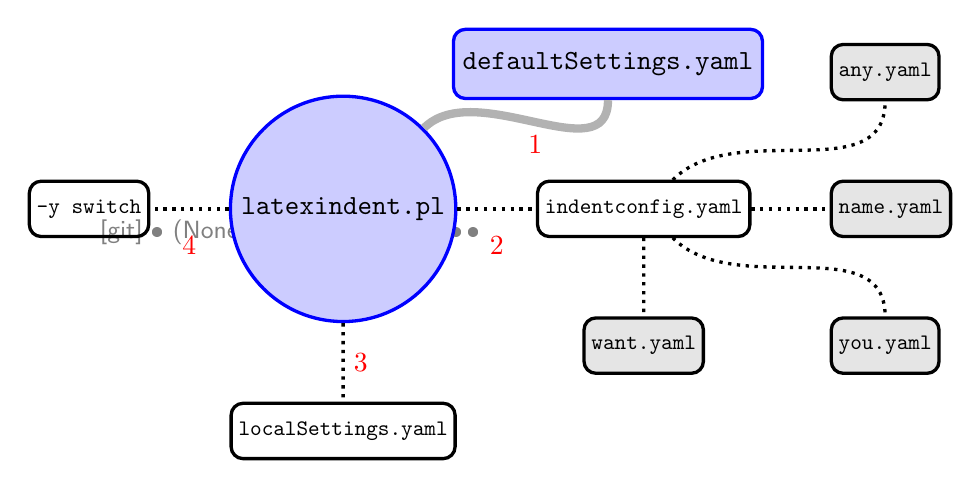
\begin{tikzpicture}[
		needed/.style={very thick, draw=blue,fill=blue!20, text centered, minimum height=2.5em,rounded corners=1ex},
		optional/.style={draw=black, very thick,scale=0.8, text centered, minimum height=2.5em,rounded corners=1ex},
		optionalfill/.style={fill=black!10},
		connections/.style={draw=black!30,dotted,line width=3pt,text=red},
	]
	% Draw diagram elements
	\node (latexindent) [needed,circle] {\texttt{latexindent.pl}};
	\node (default) [needed,above right=.5cm of latexindent] {\texttt{defaultSettings.yaml}};
	\node (indentconfig) [optional,right=of latexindent] {\texttt{indentconfig.yaml}};
	\node (any) [optional,optionalfill,above right=of indentconfig] {\texttt{any.yaml}};
	\node (name) [optional,optionalfill,right=of indentconfig] {\texttt{name.yaml}};
	\node (you) [optional,optionalfill,below right=of indentconfig] {\texttt{you.yaml}};
	\node (want) [optional,optionalfill,below=of indentconfig] {\texttt{want.yaml}};
	\node (local) [optional,below=of latexindent] {\texttt{localSettings.yaml}};
	\node (yamlswitch) [optional,left=of latexindent] {\texttt{-y switch}};
	% Draw arrows between elements
	\draw[connections,solid] (latexindent) to[in=-90]node[pos=0.5,anchor=north]{1} (default.south) ;
	\draw[connections,optional] (latexindent) -- node[pos=0.5,anchor=north]{2} (indentconfig) ;
	\draw[connections,optional] (indentconfig) to[in=-90] (any.south) ;
	\draw[connections,optional] (indentconfig) -- (name) ;
	\draw[connections,optional] (indentconfig) to[out=-45,in=90] (you) ;
	\draw[connections,optional] (indentconfig) -- (want) ;
	\draw[connections,optional] (latexindent) -- node[pos=0.5,anchor=west]{3} (local) ;
	\draw[connections,optional] (latexindent) -- node[pos=0.5,anchor=north]{4} (yamlswitch) ;
\end{tikzpicture}
\end{document}

		\caption{Schematic of the load order described in \cref{sec:loadorder}; solid lines represent
			mandatory files, dotted lines represent optional files. \texttt{indentconfig.yaml} can
			contain as many files as you like. The files will be loaded in order; if you specify
			settings for the same field in more than one file, the most recent takes priority. }
		\label{fig:loadorder}
	\end{figure}

 % arara: pdflatex: { files: [latexindent]}
\section{defaultSettings.yaml}\label{sec:defuseloc}
 \texttt{latexindent.pl} loads its settings from \texttt{defaultSettings.yaml}. The idea
 is to separate the behaviour of the script from the internal working -- this is very
 similar to the way that we separate content from form when writing our documents in
 \LaTeX.

 If you look in \texttt{defaultSettings.yaml} you'll find the switches that govern the
 behaviour of \texttt{latexindent.pl}. If you're not sure where
 \texttt{defaultSettings.yaml} resides on your computer, don't worry as
 \texttt{indent.log} will tell you where to find it. \texttt{defaultSettings.yaml} is
 commented, but here is a description of what each switch is designed to do. The default
 value is given in each case; whenever you see \emph{integer} in \emph{this} section,
 assume that it must be greater than or equal to \texttt{0} unless otherwise stated.

 For most of the settings in \texttt{defaultSettings.yaml} that are specified as integers,
 then we understand \texttt{0} to represent `off' and \texttt{1} to represent `on'. For
 fields that allow values other than \texttt{0} or \texttt{1}, it is hoped that the
 specific context and associated commentary should make it clear which values are allowed.

\yamltitle{fileExtensionPreference}*{fields}
	\texttt{latexindent.pl} can be called to
	act on a file without specifying the file extension. For example we can call
	\begin{commandshell}
latexindent.pl myfile
\end{commandshell}
	in which case the script will look for \texttt{myfile} with the extensions specified in
	\texttt{fileExtensionPreference} in their numeric order. If no match is found, the script
	will exit. As with all of the fields, you should change and/or add to this as necessary.

	\cmhlistingsfromfile[style=fileExtensionPreference]{../defaultSettings.yaml}[width=.8\linewidth,before=\centering,yaml-TCB]{\texttt{fileExtensionPreference}}{lst:fileExtensionPreference}

	Calling \texttt{latexindent.pl myfile} with the (default) settings specified in
	\cref{lst:fileExtensionPreference} means that the script will first look for
	\texttt{myfile.tex}, then \texttt{myfile.sty}, \texttt{myfile.cls}, and finally
	\texttt{myfile.bib} in order\footnote{Throughout this manual, listings shown with line
		numbers represent code taken directly from \texttt{defaultSettings.yaml}.}.

	\index{backup files!extension settings}

\subsection{Backup and log file preferences}
\yamltitle{backupExtension}*{extension name}

	If you call \texttt{latexindent.pl} with the \texttt{-w} switch (to overwrite
	\texttt{myfile.tex}) then it will create a backup file before doing any indentation; the
	default extension is \texttt{.bak}, so, for example, \texttt{myfile.bak0} would be
	created when calling \texttt{latexindent.pl myfile.tex} for the first time.

	By default, every time you subsequently call \texttt{latexindent.pl} with the \texttt{-w}
	to act upon \texttt{myfile.tex}, it will create successive back up files:
	\texttt{myfile.bak1}, \texttt{myfile.bak2}, etc.

\yamltitle{onlyOneBackUp}*{integer}
	\label{page:onlyonebackup}
	\index{backup files!number of backup files}
	If you don't want a backup for every time that you call \texttt{latexindent.pl} (so you
	don't want \texttt{myfile.bak1}, \texttt{myfile.bak2}, etc) and you simply want
	\texttt{myfile.bak} (or whatever you chose \texttt{backupExtension} to be) then change
	\texttt{onlyOneBackUp} to \texttt{1}; the default value of \texttt{onlyOneBackUp} is
	\texttt{0}.
	\index{backup files!maximum number of backup files}
	\index{backup files!number of backup files}

\yamltitle{maxNumberOfBackUps}*{integer}
	Some users may only want a finite number of backup files, say at most $3$, in which case,
	they can change this switch. The smallest value of \texttt{maxNumberOfBackUps} is $0$
	which will \emph{not} prevent backup files being made; in this case, the behaviour will
	be dictated entirely by \texttt{onlyOneBackUp}. The default value of
	\texttt{maxNumberOfBackUps} is \texttt{0}.

\yamltitle{cycleThroughBackUps}*{integer}
	\index{backup files!cycle through}
	Some users may wish to cycle through backup files, by deleting the oldest backup file and
	keeping only the most recent; for example, with \texttt{maxNumberOfBackUps: 4}, and
	\texttt{cycleThroughBackUps} set to \texttt{1} then the \texttt{copy} procedure given
	below would be obeyed.

	\begin{commandshell}
copy myfile.bak1 to myfile.bak0
copy myfile.bak2 to myfile.bak1
copy myfile.bak3 to myfile.bak2
copy myfile.bak4 to myfile.bak3
\end{commandshell}
	The default value of \texttt{cycleThroughBackUps} is \texttt{0}.

\yamltitle{logFilePreferences}*{fields}
	\texttt{latexindent.pl} writes information to \texttt{indent.log}, some
	of which can be customized by changing \texttt{logFilePreferences}; see
	\cref{lst:logFilePreferences}. If you load your own user settings (see
	\vref{sec:indentconfig}) then \texttt{latexindent.pl} will detail them in
	\texttt{indent.log}; you can choose not to have the details logged by switching
	\texttt{showEveryYamlRead} to \texttt{0}. Once all of your settings have been loaded, you
	can see the amalgamated settings in the log file by switching
	\texttt{showAmalgamatedSettings} to \texttt{1}, if you wish.

	\cmhlistingsfromfile[style=logFilePreferences,]{../defaultSettings.yaml}[width=.9\linewidth,before=\centering,yaml-TCB]{\texttt{logFilePreferences}}{lst:logFilePreferences}

	When%
	\announce{2018-01-13}{showDecorationStartCodeBlockTrace feature for log file} either of
	the \texttt{trace} modes (see \cpageref{page:traceswitch}) are active, you will receive
	detailed information in \texttt{indent.log}. You can specify character strings to appear
	before and after the notification of a found code block using, respectively,
	\texttt{showDecorationStartCodeBlockTrace} and
	\texttt{showDecorationFinishCodeBlockTrace}. A demonstration is given in
	\vref{app:logfile-demo}.

	The log file will end with the characters given in \texttt{endLogFileWith}, and will
	report the \texttt{GitHub} address of \texttt{latexindent.pl} to the log file if
	\texttt{showGitHubInfoFooter} is set to \texttt{1}.

	Note: \texttt{latexindent.pl} no longer uses the \texttt{log4perl} module to handle the
	creation of the logfile.%
	\announce{2021-03-14}*{no longer using log4perl}

	Some of the options%
	\announce{2021-06-19}*{logFilePreferences updated to include Dumper options} for Perl's
	\texttt{Dumper} module can be specified in \cref{lst:logFilePreferences}; see
	\cite{dumper} and \cite{dumperdemo} for more information. These options will mostly be
	helpful for those calling \texttt{latexindent.pl} with the \texttt{-tt} option described
	in \cref{sec:commandline}.

\subsection{Verbatim code blocks}
\yamltitle{verbatimEnvironments}*{fields}

	A field that contains a list of environments that you would like left completely alone --
	no indentation will be performed on environments that you have specified in this field,
	see \cref{lst:verbatimEnvironments}.
	\index{verbatim!environments}
	\index{verbatim!commands}

	\begin{cmhtcbraster}[raster column skip=.1\linewidth]
		\cmhlistingsfromfile[style=verbatimEnvironments]{../defaultSettings.yaml}[width=.8\linewidth,before=\centering,yaml-TCB]{\texttt{verbatimEnvironments}}{lst:verbatimEnvironments}
		\cmhlistingsfromfile[style=verbatimCommands]{../defaultSettings.yaml}[width=.8\linewidth,before=\centering,yaml-TCB]{\texttt{verbatimCommands}}{lst:verbatimCommands}
	\end{cmhtcbraster}

	Note that if you put an environment in	\texttt{verbatimEnvironments} and in other fields
	such as \texttt{lookForAlignDelims} or \texttt{noAdditionalIndent} then
	\texttt{latexindent.pl} will \emph{always} prioritize \texttt{verbatimEnvironments}.

	You can, optionally, specify
	\announce*{2021-10-30}{verbatim name feature} the
	\texttt{verbatim} field using the \texttt{name} field which takes a regular expression as
	its argument; thank you to \cite{XuehaiPan} for contributing this feature.

	For demonstration, then assuming that your file contains the environments
	\texttt{latexcode}, \texttt{latexcode*}, \texttt{pythoncode} and \texttt{pythoncode*},
	then the listings given in \cref{lst:nameAsRegex1,lst:nameAsRegex2} are equivalent.

	\begin{cmhtcbraster}[raster column skip=.1\linewidth]
		\cmhlistingsfromfile*{demonstrations/nameAsRegex1.yaml}[yaml-TCB]{\texttt{nameAsRegex1.yaml}}{lst:nameAsRegex1}
		\cmhlistingsfromfile*{demonstrations/nameAsRegex2.yaml}[yaml-TCB]{\texttt{nameAsRegex2.yaml}}{lst:nameAsRegex2}
	\end{cmhtcbraster}

	With reference to \cref{lst:nameAsRegex2}:
	\begin{itemize}
		\item the \texttt{name} field as specified here means \emph{any word followed by the word code,
			      optionally followed by *};
		\item we have used \texttt{nameAsRegex} to identify this field, but you can use any description
		      you like;
		\item the \texttt{lookForThis} field is optional, and can take the values 0 (off) or 1 (on); by
		      default, it is assumed to be 1 (on).
	\end{itemize}

\yamltitle{verbatimCommands}*{fields}
	A field that contains a list of commands that are verbatim commands, for example
	\lstinline|\lstinline|; any commands populated in this field are protected from line
	breaking routines (only relevant if the \texttt{-m} is active, see
	\vref{sec:modifylinebreaks}).

	With reference to \cref{lst:verbatimCommands}, by default \texttt{latexindent.pl} looks
	for
	\lstinline|\verb| immediately followed by another character, and then it takes the
	body as anything up to the next occurrence of the character; this means that, for
	example, \lstinline|\verb!x+3!| is treated as a \texttt{verbatimCommands}.

	You can, optionally, specify
	\announce*{2021-10-30}{verbatimCommands name feature} the
	\texttt{verbatimCommands} field using the \texttt{name} field which takes a regular
	expression as its argument; thank you to \cite{XuehaiPan} for contributing this feature.

	For demonstration, then assuming that your file contains the commands
	\texttt{verbinline}, \texttt{myinline} then the listings given in
	\cref{lst:nameAsRegex3,lst:nameAsRegex4} are equivalent.

	\begin{cmhtcbraster}[raster column skip=.1\linewidth]
		\cmhlistingsfromfile*{demonstrations/nameAsRegex3.yaml}[yaml-TCB]{\texttt{nameAsRegex3.yaml}}{lst:nameAsRegex3}
		\cmhlistingsfromfile*{demonstrations/nameAsRegex4.yaml}[yaml-TCB]{\texttt{nameAsRegex4.yaml}}{lst:nameAsRegex4}
	\end{cmhtcbraster}

	With reference to \cref{lst:nameAsRegex4}:
	\begin{itemize}
		\item the \texttt{name} field as specified here means \emph{any word followed by the word
			      inline};
		\item we have used \texttt{nameAsRegex} to identify this field, but you can use any description
		      you like;
		\item the \texttt{lookForThis} field is optional, and can take the values 0 (off) or 1 (on); by
		      default, it is assumed to be 1 (on).
	\end{itemize}

\yamltitle{noIndentBlock}*{fields}
	If you have a block of code that you don't want \texttt{latexindent.pl} to touch (even if
	\index{verbatim!noIndentBlock} it is \emph{not} a verbatim-like environment) then you can
	wrap it in an environment from \texttt{noIndentBlock}; you can use any name you like for
	this, provided you populate it as demonstrate in \cref{lst:noIndentBlock}.

	\cmhlistingsfromfile[style=noIndentBlock]{../defaultSettings.yaml}[width=.4\linewidth,before=\centering,yaml-TCB]{\texttt{noIndentBlock}}{lst:noIndentBlock}

	Of course, you don't want to have to specify these as null environments in your code, so
	you use them with a comment symbol, \lstinline!%!, followed by as many spaces (possibly
	none) as you like; see \cref{lst:noIndentBlockdemo} for example.

	\cmhlistingsfromfile{demonstrations/noindentblock.tex}{\texttt{noIndentBlock.tex}}{lst:noIndentBlockdemo}

	Important note: it is assumed that the \texttt{noindent} block statements specified in
	this way appear on their own line.

	The%
	\announce{2021-06-19}{noIndentBlock specified as regex} \texttt{noIndentBlock} fields can also be specified in terms of \texttt{begin} and
	\texttt{end} fields. We use the code in \cref{lst:noIndentBlock1} to demonstrate this
	feature.

	\cmhlistingsfromfile{demonstrations/noindentblock1.tex}{\texttt{noIndentBlock1.tex}}{lst:noIndentBlock1}

	The settings given in \cref{lst:noindent1,lst:noindent2} are equivalent:

	\begin{cmhtcbraster}[raster columns=3,
			raster left skip=-3.5cm,
			raster right skip=-2cm,
			raster column skip=.03\linewidth]
		\cmhlistingsfromfile{demonstrations/noindent1.yaml}[yaml-TCB]{\texttt{noindent1.yaml}}{lst:noindent1}
		\cmhlistingsfromfile{demonstrations/noindent2.yaml}[yaml-TCB]{\texttt{noindent2.yaml}}{lst:noindent2}
		\cmhlistingsfromfile{demonstrations/noindent3.yaml}[yaml-TCB]{\texttt{noindent3.yaml}}{lst:noindent3}
	\end{cmhtcbraster}

	Upon running the commands
	\begin{commandshell}
latexindent.pl -l noindent1.yaml noindent1
latexindent.pl -l noindent2.yaml noindent1
\end{commandshell}
	then we receive the output given in \cref{lst:noIndentBlock1-mod1}.

	\cmhlistingsfromfile{demonstrations/noindentblock1-mod1.tex}{\texttt{noIndentBlock1.tex} using \cref{lst:noindent1} or \cref{lst:noindent2}}{lst:noIndentBlock1-mod1}

	The \texttt{begin}, \texttt{body} and \texttt{end} fields for \texttt{noIndentBlock} are
	all \emph{regular expressions}. If the \texttt{body} field is not specified, then it
	takes a default value of
	\lstinline!.*?! which is written explicitly in \cref{lst:noindent1}. In this
	context, we interpret \lstinline!.*?! in words as \emph{the fewest number of characters
		(possibly none) until the `end' field is reached}.

	The \texttt{lookForThis} field is optional, and can take the values 0 (off) or 1 (on); by
	default, it is assumed to be 1 (on).

	Using \cref{lst:noindent3} demonstrates setting \texttt{lookForThis} to 0 (off); running
	the command
	\begin{commandshell}
latexindent.pl -l noindent3.yaml noindent1
\end{commandshell}
	gives the output in \cref{lst:noIndentBlock1-mod3}.

	\cmhlistingsfromfile{demonstrations/noindentblock1-mod3.tex}{\texttt{noIndentBlock1.tex} using \cref{lst:noindent3}}{lst:noIndentBlock1-mod3}

	We will demonstrate this feature later in the documentation in \cref{lst:href3}.

	You can, optionally, specify
	\announce*{2021-10-30}{noIndentBlock name feature} the
	\texttt{noIndentBlock} field using the \texttt{name} field which takes a regular
	expression as its argument; thank you to \cite{XuehaiPan} for contributing this feature.

	For demonstration, then assuming that your file contains the environments
	\texttt{testnoindent}, \texttt{testnoindent*} then the listings given in
	\cref{lst:nameAsRegex5,lst:nameAsRegex6} are equivalent.

	\begin{widepage}
		\begin{cmhtcbraster}[raster column skip=.1\linewidth]
			\cmhlistingsfromfile*{demonstrations/nameAsRegex5.yaml}[yaml-TCB]{\texttt{nameAsRegex5.yaml}}{lst:nameAsRegex5}
			\cmhlistingsfromfile*{demonstrations/nameAsRegex6.yaml}[yaml-TCB]{\texttt{nameAsRegex6.yaml}}{lst:nameAsRegex6}
		\end{cmhtcbraster}
	\end{widepage}

	With reference to \cref{lst:nameAsRegex6}:
	\begin{itemize}
		\item the \texttt{name} field as specified here means \emph{any word followed by the word
			      noindent, optionally followed by *};
		\item we have used \texttt{nameAsRegex} to identify this field, but you can use any description
		      you like;
		\item the \texttt{lookForThis} field is optional, and can take the values 0 (off) or 1 (on); by
		      default, it is assumed to be 1 (on).
	\end{itemize}
\subsection{filecontents and preamble}
\yamltitle{fileContentsEnvironments}*{field}

	Before \texttt{latexindent.pl} determines the difference between preamble (if any) and
	the main document, it first searches for any of the environments specified in
	\texttt{fileContentsEnvironments}, see \cref{lst:fileContentsEnvironments}. The behaviour
	of \texttt{latexindent.pl} on these environments is determined by their location
	(preamble or not), and the value \texttt{indentPreamble}, discussed next.

	\cmhlistingsfromfile[style=fileContentsEnvironments]{../defaultSettings.yaml}[width=.8\linewidth,before=\centering,yaml-TCB]{\texttt{fileContentsEnvironments}}{lst:fileContentsEnvironments}

\yamltitle{indentPreamble}{0|1}

	The preamble of a document can sometimes contain some trickier code for
	\texttt{latexindent.pl} to operate upon. By default, \texttt{latexindent.pl} won't try to
	operate on the preamble (as \texttt{indentPreamble} is set to \texttt{0}, by default),
	but if you'd like \texttt{latexindent.pl} to try then change \texttt{indentPreamble} to
	\texttt{1}.

\yamltitle{lookForPreamble}*{fields}

	Not all files contain preamble; for example, \texttt{sty}, \texttt{cls} and \texttt{bib}
	files typically do \emph{not}. Referencing \cref{lst:lookForPreamble}, if you set, for
	example, \texttt{.tex} to \texttt{0}, then regardless of the setting of the value of
	\texttt{indentPreamble}, preamble will not be assumed when operating upon \texttt{.tex}
	files.

	\cmhlistingsfromfile[style=lookForPreamble]{../defaultSettings.yaml}[width=.8\linewidth,before=\centering,yaml-TCB]{lookForPreamble}{lst:lookForPreamble}
\yamltitle{preambleCommandsBeforeEnvironments}{0|1}
	Assuming that \texttt{latexindent.pl} is asked to operate upon the preamble of a
	document, when this switch is set to \texttt{0} then environment code blocks will be
	sought first, and then command code blocks. When this switch is set to \texttt{1},
	commands will be sought first. The example that first motivated this switch contained the
	code given in \cref{lst:motivatepreambleCommandsBeforeEnvironments}.

	\begin{cmhlistings}{Motivating \texttt{preambleCommandsBeforeEnvironments}}{lst:motivatepreambleCommandsBeforeEnvironments}
...
preheadhook={\begin{mdframed}[style=myframedstyle]},
postfoothook=\end{mdframed},
...
\end{cmhlistings}

	\index{indentation!defaultIndent description}

\subsection{Indentation and horizontal space}
\yamltitle{defaultIndent}*{horizontal space}
	This is the default indentation used in the absence of other details for the code block
	with which we are working. The default value is \lstinline!\t! which means a tab; we will
	explore customisation beyond \texttt{defaultIndent} in \vref{sec:noadd-indent-rules}.

	If you're interested in experimenting with \texttt{latexindent.pl} then you can
	\emph{remove} all indentation by setting \texttt{defaultIndent: ""}.

\yamltitle{removeTrailingWhitespace}*{fields}\label{yaml:removeTrailingWhitespace}

	Trailing white space can be removed both \emph{before} and \emph{after} processing the
	document, as detailed in \cref{lst:removeTrailingWhitespace}; each of the fields can take
	the values \texttt{0} or \texttt{1}. See
	\vref{lst:removeTWS-before,lst:env-mlb5-modAll,lst:env-mlb5-modAll-remove-WS} for before
	and after results. Thanks to \cite{vosskuhle} for providing this feature.

	\begin{minipage}{.4\textwidth}
		\cmhlistingsfromfile[style=removeTrailingWhitespace]{../defaultSettings.yaml}[before=\centering,yaml-TCB]{removeTrailingWhitespace}{lst:removeTrailingWhitespace}
	\end{minipage}%
	\hfill
	\begin{minipage}{.5\textwidth}
		\begin{yaml}[numbers=none]{removeTrailingWhitespace (alt)}[before=\centering]{lst:removeTrailingWhitespace-alt}
removeTrailingWhitespace: 1
\end{yaml}
	\end{minipage}%

	You can specify \texttt{removeTrailingWhitespace} simply as \texttt{0} or \texttt{1}, if
	you wish; in this case,%
	\announce{2017-06-28}{removeTrailingWhitespace} \texttt{latexindent.pl} will set both
	\texttt{beforeProcessing} and \texttt{afterProcessing} to the value you specify; see
	\cref{lst:removeTrailingWhitespace-alt}.

\subsection{Aligning at delimiters}
\yamltitle{lookForAlignDelims}*{fields}
	This contains a list of code blocks that are operated upon in a special way by
	\texttt{latexindent.pl} (see \cref{lst:aligndelims:basic}). In fact, the fields in
	\texttt{lookForAlignDelims} can actually take two different forms: the \emph{basic}
	version is shown in \cref{lst:aligndelims:basic} and the \emph{advanced} version in
	\cref{lst:aligndelims:advanced}; we will discuss each in turn.
	\index{delimiters!advanced settings of lookForAlignDelims}

	\begin{yaml}[numbers=none]{\texttt{lookForAlignDelims} (basic)}[width=.8\linewidth,before=\centering]{lst:aligndelims:basic}
lookForAlignDelims:
   tabular: 1
   tabularx: 1
   longtable: 1
   array: 1
   matrix: 1
   ...
	\end{yaml}

	Specifying code blocks in this field instructs \texttt{latexindent.pl} to try and align
	each column by its alignment delimiters. It does have some limitations (discussed further
	in \cref{sec:knownlimitations}), but in many cases it will produce results such as those
	in \cref{lst:tabularbefore:basic,lst:tabularafter:basic}.

	If you find that \texttt{latexindent.pl} does not perform satisfactorily on such
	environments then you can set the relevant key to \texttt{0}, for example
	\texttt{tabular: 0}; alternatively, if you just want to ignore \emph{specific} instances
	of the environment, you could wrap them in something from \texttt{noIndentBlock} (see
	\vref{lst:noIndentBlock}).

	\begin{cmhtcbraster}
		\cmhlistingsfromfile{demonstrations/tabular1.tex}{\texttt{tabular1.tex}}{lst:tabularbefore:basic}
		\cmhlistingsfromfile{demonstrations/tabular1-default.tex}{\texttt{tabular1.tex} default output}{lst:tabularafter:basic}
	\end{cmhtcbraster}

	If, for example, you wish to remove the alignment of the \lstinline!\\! within a
	delimiter-aligned block, then the advanced form of \texttt{lookForAlignDelims} shown in
	\cref{lst:aligndelims:advanced} is for you.
	\index{regular expressions!delimiterRegEx}
	\index{regular expressions!ampersand alignment}
	\index{delimiters!default settings of lookForAlignDelims}
	\index{delimiters!ampersand \&}
	\index{delimiters!advanced settings}
	\index{delimiters!lookForAlignDelims}

	\cmhlistingsfromfile[style=lookForAlignDelims]{../defaultSettings.yaml}[width=.8\linewidth,before=\centering,yaml-TCB]{\texttt{lookForAlignDelims} (advanced)}{lst:aligndelims:advanced}

	Note that you can use a mixture of the basic and advanced form: in
	\cref{lst:aligndelims:advanced} \texttt{tabular} and \texttt{tabularx} are advanced and
	\texttt{longtable} is basic. When using the advanced form, each field should receive at
	least 1 sub-field, and \emph{can} (but does not have to) receive any of the following
	fields:
	\begin{itemize}
		\item \texttt{delims}: binary switch (0 or 1) equivalent to simply specifying, for
		      example, \texttt{tabular: 1} in the basic version shown in \cref{lst:aligndelims:basic}.
		      If \texttt{delims} is set to \texttt{0} then the align at ampersand routine will not be
		      called for this code block (default: 1);
		\item \texttt{alignDoubleBackSlash}: binary switch (0 or 1) to determine if
		      \lstinline!\\!
		      should be aligned (default: 1);
		\item \texttt{spacesBeforeDoubleBackSlash}: optionally,%
		      \announce{2018-01-13}*{update to spacesBeforeDoubleBackSlash in ampersand alignment}
		      specifies the number (integer $\geq$ 0) of spaces to be inserted before
		      \lstinline!\\! (default: 1); %\footnote{Previously this only activated if \texttt{alignDoubleBackSlash} was set to \texttt{0}.}
		\item \announce{2017-06-19}{multiColumnGrouping} \texttt{multiColumnGrouping}: binary switch (0
		      or 1) that details if \texttt{latexindent.pl} should group columns above and below a
		      \lstinline!\multicolumn! command (default: 0);
		\item \announce{2017-06-19}{alignRowsWithoutMaxDelims} \texttt{alignRowsWithoutMaxDelims}:
		      binary switch (0 or 1) that details if rows that do not contain the maximum number of
		      delimeters should be formatted so as to have the ampersands aligned (default: 1);
		\item \announce{2018-01-13}{spacesBeforeAmpersand in ampersand alignment}\texttt{spacesBeforeAmpersand}: optionally specifies the number (integer $\geq$
		      0) of spaces to be placed \emph{before} ampersands (default: 1);
		\item \announce{2018-01-13}{spacesAfterAmpersand in ampersand alignment}\texttt{spacesAfterAmpersand}: optionally specifies the number (integer $\geq$
		      0) of spaces to be placed \emph{After} ampersands (default: 1);
		\item \announce{2018-01-13}{justification of cells in ampersand alignment}\texttt{justification}: optionally specifies the justification of each cell as
		      either \emph{left} or \emph{right} (default: left);
		\item \announce{2020-03-21}{align final double back slash}{alignFinalDoubleBackSlash}
		      optionally specifies if the \emph{final} double back slash should be used for alignment
		      (default: 0);
		\item \announce{2020-03-21}{don't measure feature}{dontMeasure} optionally specifies if
		      user-specified cells, rows or the largest entries should \emph{not} be measured (default:
		      0);
		\item \announce{2020-03-21}{delimiter RegEx feature}{delimiterRegEx} optionally specifies the
		      pattern matching to be used for the alignment delimeter (default:
		      \lstinline* '(?<!\\)(&)'*);
		\item \announce{2020-03-21}{delimiter justification}{delimiterJustification} optionally
		      specifies the justification for the alignment delimeters (default: left); note that this
		      feature is only useful if you have delimiters of different lengths in the same column,
		      discussed in \cref{sec:delimiter-reg-ex}.
	\end{itemize}

	We will explore most of these features using the file \texttt{tabular2.tex} in
	\cref{lst:tabular2} (which contains a \lstinline!\multicolumn! command), and the YAML
	files in \crefrange{lst:tabular2YAML}{lst:tabular8YAML}; we will explore
	\texttt{alignFinalDoubleBackSlash} in \cref{lst:tabular4}; the \texttt{dontMeasure}
	feature will be described in \cref{sec:dontMeasure}, and \texttt{delimiterRegEx} in
	\cref{sec:delimiter-reg-ex}.

	\cmhlistingsfromfile{demonstrations/tabular2.tex}{\texttt{tabular2.tex}}{lst:tabular2}
	\begin{minipage}{.45\textwidth}
		\cmhlistingsfromfile[style=yaml-LST]{demonstrations/tabular2.yaml}[yaml-TCB]{\texttt{tabular2.yaml}}{lst:tabular2YAML}
	\end{minipage}%
	\hfill
	\begin{minipage}{.48\textwidth}
		\cmhlistingsfromfile[style=yaml-LST]{demonstrations/tabular3.yaml}[yaml-TCB]{\texttt{tabular3.yaml}}{lst:tabular3YAML}
	\end{minipage}%

	\begin{minipage}{.45\textwidth}
		\cmhlistingsfromfile[style=yaml-LST]{demonstrations/tabular4.yaml}[yaml-TCB]{\texttt{tabular4.yaml}}{lst:tabular4YAML}
	\end{minipage}%
	\hfill
	\begin{minipage}{.48\textwidth}
		\cmhlistingsfromfile[style=yaml-LST]{demonstrations/tabular5.yaml}[yaml-TCB]{\texttt{tabular5.yaml}}{lst:tabular5YAML}
	\end{minipage}%

	\begin{minipage}{.45\textwidth}
		\cmhlistingsfromfile[style=yaml-LST]{demonstrations/tabular6.yaml}[yaml-TCB]{\texttt{tabular6.yaml}}{lst:tabular6YAML}
	\end{minipage}%
	\hfill
	\begin{minipage}{.48\textwidth}
		\cmhlistingsfromfile[style=yaml-LST]{demonstrations/tabular7.yaml}[yaml-TCB]{\texttt{tabular7.yaml}}{lst:tabular7YAML}
	\end{minipage}%

	\begin{minipage}{.48\textwidth}
		\cmhlistingsfromfile[style=yaml-LST]{demonstrations/tabular8.yaml}[yaml-TCB]{\texttt{tabular8.yaml}}{lst:tabular8YAML}
	\end{minipage}%

	On running the commands
	\index{delimiters!spacing demonstration}
	\index{switches!-l demonstration}
	\begin{commandshell}
latexindent.pl tabular2.tex 
latexindent.pl tabular2.tex -l tabular2.yaml
latexindent.pl tabular2.tex -l tabular3.yaml
latexindent.pl tabular2.tex -l tabular2.yaml,tabular4.yaml
latexindent.pl tabular2.tex -l tabular2.yaml,tabular5.yaml
latexindent.pl tabular2.tex -l tabular2.yaml,tabular6.yaml
latexindent.pl tabular2.tex -l tabular2.yaml,tabular7.yaml
latexindent.pl tabular2.tex -l tabular2.yaml,tabular8.yaml
\end{commandshell}
	we obtain the respective outputs given in
	\crefrange{lst:tabular2-default}{lst:tabular2-mod8}.

	\begin{widepage}
		\cmhlistingsfromfile{demonstrations/tabular2-default.tex}{\texttt{tabular2.tex} default output}{lst:tabular2-default}
		\cmhlistingsfromfile{demonstrations/tabular2-mod2.tex}{\texttt{tabular2.tex} using \cref{lst:tabular2YAML}}{lst:tabular2-mod2}
		\cmhlistingsfromfile{demonstrations/tabular2-mod3.tex}{\texttt{tabular2.tex} using \cref{lst:tabular3YAML}}{lst:tabular2-mod3}
		\cmhlistingsfromfile{demonstrations/tabular2-mod4.tex}{\texttt{tabular2.tex} using \cref{lst:tabular2YAML,lst:tabular4YAML}}{lst:tabular2-mod4}
		\cmhlistingsfromfile{demonstrations/tabular2-mod5.tex}{\texttt{tabular2.tex} using \cref{lst:tabular2YAML,lst:tabular5YAML}}{lst:tabular2-mod5}
		\cmhlistingsfromfile{demonstrations/tabular2-mod6.tex}{\texttt{tabular2.tex} using \cref{lst:tabular2YAML,lst:tabular6YAML}}{lst:tabular2-mod6}
		\cmhlistingsfromfile{demonstrations/tabular2-mod7.tex}{\texttt{tabular2.tex} using \cref{lst:tabular2YAML,lst:tabular7YAML}}{lst:tabular2-mod7}
		\cmhlistingsfromfile{demonstrations/tabular2-mod8.tex}{\texttt{tabular2.tex} using \cref{lst:tabular2YAML,lst:tabular8YAML}}{lst:tabular2-mod8}
	\end{widepage}

	Notice in particular:
	\begin{itemize}
		\item in both \cref{lst:tabular2-default,lst:tabular2-mod2} all rows have been aligned at the
		      ampersand, even those that do not contain the maximum number of ampersands (3 ampersands,
		      in this case);
		\item in \cref{lst:tabular2-default} the columns have been aligned at the ampersand;
		\item in \cref{lst:tabular2-mod2} the \lstinline!\multicolumn! command has grouped the $2$
		      columns beneath \emph{and} above it, because \texttt{multiColumnGrouping} is set to $1$
		      in \cref{lst:tabular2YAML};
		\item in \cref{lst:tabular2-mod3} rows~3 and~6 have \emph{not} been aligned at the ampersand,
		      because \texttt{alignRowsWithoutMaxDelims} has been to set to $0$ in
		      \cref{lst:tabular3YAML}; however, the \lstinline!\\! \emph{have} still been aligned;
		\item in \cref{lst:tabular2-mod4} the columns beneath and above the \lstinline!\multicolumn!
		      commands have been grouped (because \texttt{multiColumnGrouping} is set to $1$), and
		      there are at least $4$ spaces \emph{before} each aligned ampersand because
		      \texttt{spacesBeforeAmpersand} is set to $4$;
		\item in \cref{lst:tabular2-mod5} the columns beneath and above the \lstinline!\multicolumn!
		      commands have been grouped (because \texttt{multiColumnGrouping} is set to $1$), and
		      there are at least $4$ spaces \emph{after} each aligned ampersand because
		      \texttt{spacesAfterAmpersand} is set to $4$;
		\item in \cref{lst:tabular2-mod6} the \lstinline!\\! have \emph{not} been aligned, because
		      \texttt{alignDoubleBackSlash} is set to \texttt{0}, otherwise the output is the same as
		      \cref{lst:tabular2-mod2};
		\item in \cref{lst:tabular2-mod7} the \lstinline!\\! \emph{have} been aligned, and because
		      \texttt{spacesBeforeDoubleBackSlash} is set to \texttt{0}, there are no spaces ahead of
		      them; the output is otherwise the same as \cref{lst:tabular2-mod2};
		\item in \cref{lst:tabular2-mod8} the cells have been \emph{right}-justified; note that cells
		      above and below the \lstinline!\multicol! statements have still been group correctly,
		      because of the settings in \cref{lst:tabular2YAML}.
	\end{itemize}

\subsubsection{lookForAlignDelims: spacesBeforeAmpersand}
	The \texttt{spacesBeforeAmpersand}%
	\announce{2021-06-19}*{spacesBeforeAmpersand leading blank column upgrade} can be
	specified in a few different ways. The \emph{basic} form is demonstrated in
	\cref{lst:tabular4YAML}, but we can customise the behaviour further by specifying if we
	would like this value to change if it encounters a \emph{leading blank column}; that is,
	when the first column contains only zero-width entries. We refer to this as the
	\emph{advanced} form.

	We demonstrate this feature in relation to \cref{lst:aligned1}; upon running the
	following command
	\begin{commandshell}
latexindent.pl aligned1.tex -o=+-default
\end{commandshell}
	then we receive the default output given in \cref{lst:aligned1-default}.

	\begin{cmhtcbraster}
		\cmhlistingsfromfile{demonstrations/aligned1.tex}{\texttt{aligned1.tex}}{lst:aligned1}
		\cmhlistingsfromfile{demonstrations/aligned1-default.tex}{\texttt{aligned1-default.tex}}{lst:aligned1-default}
	\end{cmhtcbraster}

	The settings in \crefrange{lst:sba1}{lst:sba4} are all equivlanent; we have used the
	not-yet discussed \texttt{noAdditionalIndent} field (see \vref{sec:noadd-indent-rules})
	which will assist in the demonstration in what follows.
	\begin{cmhtcbraster}[raster columns=2, ]
		\cmhlistingsfromfile{demonstrations/sba1.yaml}[yaml-TCB]{\texttt{sba1.yaml}}{lst:sba1}
		\cmhlistingsfromfile{demonstrations/sba2.yaml}[yaml-TCB]{\texttt{sba2.yaml}}{lst:sba2}
		\cmhlistingsfromfile{demonstrations/sba3.yaml}[yaml-TCB]{\texttt{sba3.yaml}}{lst:sba3}
		\cmhlistingsfromfile{demonstrations/sba4.yaml}[yaml-TCB]{\texttt{sba4.yaml}}{lst:sba4}
	\end{cmhtcbraster}
	Upon running the following commands
	\begin{commandshell}
latexindent.pl aligned1.tex -l sba1.yaml
latexindent.pl aligned1.tex -l sba2.yaml
latexindent.pl aligned1.tex -l sba3.yaml
latexindent.pl aligned1.tex -l sba4.yaml
\end{commandshell}
	then we receive the (same) output given in \cref{lst:aligned1-mod1}; we note that there
	is \emph{one space} before each ampersand.

	\begin{cmhtcbraster}
		\cmhlistingsfromfile{demonstrations/aligned1-mod1.tex}{\texttt{aligned1-mod1.tex}}{lst:aligned1-mod1}
	\end{cmhtcbraster}

	We note in particular:
	\begin{itemize}
		\item \cref{lst:sba1} demonstrates the \emph{basic} form for
		      \texttt{lookForAlignDelims}; in this case,
		      the default values are specified as in \vref{lst:aligndelims:advanced};
		\item \cref{lst:sba2} demonstrates the \emph{advanced} form for
		      \texttt{lookForAlignDelims}
		      and specified \texttt{spacesBeforeAmpersand}. The default value is \texttt{1};
		\item \cref{lst:sba3} demonstrates the new \emph{advanced} way to specify
		      \texttt{spacesBeforeAmpersand}, and
		      for us to set the \texttt{default} value that sets the number of spaces before ampersands
		      which are \emph{not} in leading blank columns. The default value is \texttt{1}.

		      We note that \texttt{leadingBlankColumn} has not been specified in \cref{lst:sba3}, and
		      it will inherit the value from \texttt{default};
		\item \cref{lst:sba4} demonstrates spaces to be used before amperands for
		      \emph{leading blank columns}.
		      We note that \emph{default} has not been specified, and it will be set to \texttt{1} by
		      default.
	\end{itemize}
	We can customise the space before the ampersand in the \emph{leading blank column} of
	\cref{lst:aligned1-mod1} by using either of \cref{lst:sba5,lst:sba6}, which are
	equivalent.

	\begin{cmhtcbraster}
		\cmhlistingsfromfile{demonstrations/sba5.yaml}[yaml-TCB]{\texttt{sba5.yaml}}{lst:sba5}
		\cmhlistingsfromfile{demonstrations/sba6.yaml}[yaml-TCB]{\texttt{sba6.yaml}}{lst:sba6}
	\end{cmhtcbraster}

	Upon running
	\begin{commandshell}
latexindent.pl aligned1.tex -l sba5.yaml
latexindent.pl aligned1.tex -l sba6.yaml
\end{commandshell}
	then we receive the (same) output given in \cref{lst:aligned1-mod5}. We note that the
	space before the ampersand in the \emph{leading blank column} has been set to \texttt{0}
	by \cref{lst:sba6}.

	We can demonstrated this feature further using the settings in \cref{lst:sba7} which give
	the output in \cref{lst:aligned1-mod7}.

	\begin{cmhtcbraster}[raster columns=3,
			raster left skip=-3.75cm,
			raster right skip=-2cm,]
		\cmhlistingsfromfile{demonstrations/aligned1-mod5.tex}{\texttt{aligned1-mod5.tex}}{lst:aligned1-mod5}
		\cmhlistingsfromfile{demonstrations/aligned1-mod7.tex}{\texttt{aligned1.tex} using \cref{lst:sba7}}{lst:aligned1-mod7}
		\cmhlistingsfromfile{demonstrations/sba7.yaml}[yaml-TCB]{\texttt{sba7.yaml}}{lst:sba7}
	\end{cmhtcbraster}
\subsubsection{lookForAlignDelims: alignFinalDoubleBackSlash}
	We explore%
	\announce{2020-03-21}{alignFinalDoubleBackSlash demonstration} the
	\texttt{alignFinalDoubleBackSlash} feature by using the file in \cref{lst:tabular4}. Upon
	running the following commands
	\index{delimiters!double backslash demonstration}
	\index{switches!-y demonstration}
	\index{switches!-o demonstration}
	\begin{commandshell}
latexindent.pl tabular4.tex -o=+-default
latexindent.pl tabular4.tex -o=+-FDBS -y="lookForAlignDelims:tabular:alignFinalDoubleBackSlash:1"
\end{commandshell}
	then we receive the respective outputs given in \cref{lst:tabular4-default} and
	\cref{lst:tabular4-FDBS}.

	\begin{cmhtcbraster}[raster columns=3,
			raster left skip=-3.75cm,
			raster right skip=-2cm,]
		\cmhlistingsfromfile{demonstrations/tabular4.tex}{\texttt{tabular4.tex}}{lst:tabular4}
		\cmhlistingsfromfile{demonstrations/tabular4-default.tex}{\texttt{tabular4-default.tex}}{lst:tabular4-default}
		\cmhlistingsfromfile{demonstrations/tabular4-FDBS.tex}{\texttt{tabular4-FDBS.tex}}{lst:tabular4-FDBS}
	\end{cmhtcbraster}

	We note that in:
	\begin{itemize}
		\item \cref{lst:tabular4-default}, by default, the \emph{first} set of double back
		      slashes in the first row of the \texttt{tabular} environment have been used for
		      alignment;
		\item \cref{lst:tabular4-FDBS}, the \emph{final} set of double back slashes in the
		      first row have been used, because we specified \texttt{alignFinalDoubleBackSlash} as 1.
	\end{itemize}

	As of Version 3.0, the alignment routine works on mandatory and optional arguments within
	commands, and also within `special' code blocks (see \texttt{specialBeginEnd} on
	\cpageref{yaml:specialBeginEnd}); for example, assuming that you have a command called
	\lstinline!\matrix! and that it is populated within \texttt{lookForAlignDelims}
	(which it is, by default), and that
	you run the command
	\begin{commandshell}
latexindent.pl matrix1.tex 
\end{commandshell}
	then the before-and-after results shown in \cref{lst:matrixbefore,lst:matrixafter} are
	achievable by default.

	\begin{cmhtcbraster}
		\cmhlistingsfromfile{demonstrations/matrix1.tex}{\texttt{matrix1.tex}}{lst:matrixbefore}
		\cmhlistingsfromfile{demonstrations/matrix1-default.tex}{\texttt{matrix1.tex} default output}{lst:matrixafter}
	\end{cmhtcbraster}

	If you have blocks of code that you wish to align at the \&  character that are
	\emph{not} wrapped in, for example, \lstinline!\begin{tabular}! \ldots
	\lstinline!\end{tabular}!, then you can use the mark up illustrated in
	\cref{lst:alignmentmarkup}; the default output is shown in
	\cref{lst:alignmentmarkup-default}. Note
	that the \lstinline!%*! must be next to each other, but that there can be any number of
	spaces (possibly none) between the
	\lstinline!*! and \lstinline!\begin{tabular}!; note also that you may use any
	environment name that you have specified in \texttt{lookForAlignDelims}.

	\begin{cmhtcbraster}[raster left skip=-1.5cm,]
		\cmhlistingsfromfile{demonstrations/align-block.tex}{\texttt{align-block.tex}}{lst:alignmentmarkup}
		\cmhlistingsfromfile{demonstrations/align-block-default.tex}{\texttt{align-block.tex} default output}{lst:alignmentmarkup-default}
	\end{cmhtcbraster}

	With reference to \vref{tab:code-blocks} and the, yet undiscussed, fields of
	\texttt{noAdditionalIndent} and \texttt{indentRules} (see \vref{sec:noadd-indent-rules}),
	these comment-marked blocks are considered \texttt{environments}.

\subsubsection{lookForAlignDelims: the dontMeasure feature}\label{sec:dontMeasure}
	The%
	\announce{2020-03-21}{don't measure feature}
	\texttt{lookForAlignDelims} field can, optionally, receive the \texttt{dontMeasure}
	option which can be specified in a few different ways. We will explore this feature in
	relation to the code given in \cref{lst:tabular-DM}; the default output is shown in
	\cref{lst:tabular-DM-default}.
	\index{delimiters!dontMeasure feature}

	\begin{cmhtcbraster}[raster left skip=-1.5cm,]
		\cmhlistingsfromfile{demonstrations/tabular-DM.tex}{\texttt{tabular-DM.tex}}{lst:tabular-DM}
		\cmhlistingsfromfile{demonstrations/tabular-DM-default.tex}{\texttt{tabular-DM.tex} default output}{lst:tabular-DM-default}
	\end{cmhtcbraster}

	The \texttt{dontMeasure} field can be specified as \texttt{largest}, and in which case,
	the largest element will not be measured; with reference to the YAML file given in
	\cref{lst:dontMeasure1}, we can run the command
	\index{switches!-l demonstration}
	\begin{commandshell} 
latexindent.pl tabular-DM.tex -l=dontMeasure1.yaml
\end{commandshell}
	and receive the output given in \cref{lst:tabular-DM-mod1}.

	\begin{cmhtcbraster}
		\cmhlistingsfromfile{demonstrations/tabular-DM-mod1.tex}{\texttt{tabular-DM.tex} using \cref{lst:dontMeasure1}}{lst:tabular-DM-mod1}
		\cmhlistingsfromfile{demonstrations/dontMeasure1.yaml}[yaml-TCB]{\texttt{dontMeasure1.yaml}}{lst:dontMeasure1}
	\end{cmhtcbraster}

	We note that the \emph{largest} column entries have not contributed to the measuring
	routine.

	The \texttt{dontMeasure} field can also be specified in the form demonstrated in
	\cref{lst:dontMeasure2}. On running the following commands,
	\index{switches!-l demonstration}
	\begin{commandshell} 
latexindent.pl tabular-DM.tex -l=dontMeasure2.yaml
\end{commandshell}
	we receive the output in \cref{lst:tabular-DM-mod2}.
	\index{regular expressions!dontMeasure feature, cell}

	\begin{cmhtcbraster}
		\cmhlistingsfromfile{demonstrations/tabular-DM-mod2.tex}{\texttt{tabular-DM.tex} using \cref{lst:dontMeasure2} or \cref{lst:dontMeasure3}}{lst:tabular-DM-mod2}
		\cmhlistingsfromfile{demonstrations/dontMeasure2.yaml}[yaml-TCB]{\texttt{dontMeasure2.yaml}}{lst:dontMeasure2}
	\end{cmhtcbraster}

	We note that in \cref{lst:dontMeasure2} we have specified entries not to be measured, one
	entry per line.

	The \texttt{dontMeasure} field can also be specified in the forms demonstrated in
	\cref{lst:dontMeasure3} and \cref{lst:dontMeasure4}. Upon running the commands
	\index{switches!-l demonstration}
	\begin{commandshell} 
latexindent.pl tabular-DM.tex -l=dontMeasure3.yaml
latexindent.pl tabular-DM.tex -l=dontMeasure4.yaml
\end{commandshell}
	we receive the output given in \cref{lst:tabular-DM-mod3}
	\index{regular expressions!lowercase alph a-z}
	\begin{cmhtcbraster}[raster columns=3,
			raster left skip=-3.5cm,
			raster right skip=-2cm,
			raster column skip=.03\linewidth]
		\cmhlistingsfromfile{demonstrations/tabular-DM-mod3.tex}{\texttt{tabular-DM.tex} using \cref{lst:dontMeasure3} or \cref{lst:dontMeasure3}}{lst:tabular-DM-mod3}
		\cmhlistingsfromfile{demonstrations/dontMeasure3.yaml}[yaml-TCB]{\texttt{dontMeasure3.yaml}}{lst:dontMeasure3}
		\cmhlistingsfromfile{demonstrations/dontMeasure4.yaml}[yaml-TCB]{\texttt{dontMeasure4.yaml}}{lst:dontMeasure4}
	\end{cmhtcbraster}
	We note that in:
	\begin{itemize}
		\item \cref{lst:dontMeasure3} we have specified entries not to be measured, each one has a
		      \emph{string} in the \texttt{this}
		      field, together with an optional specification of \texttt{applyTo} as \texttt{cell};
		\item \cref{lst:dontMeasure4} we have specified entries not to be measured as a
		      \emph{regular expression} using
		      the \texttt{regex} field, together with an optional specification of \texttt{applyTo} as
		      \texttt{cell} field, together with an optional specification of \texttt{applyTo} as
		      \texttt{cell}.
	\end{itemize}
	In both cases, the default value of \texttt{applyTo} is \texttt{cell}, and does not need
	to be specified.

	We may also specify the \texttt{applyTo} field as \texttt{row}, a demonstration of which
	is given in \cref{lst:dontMeasure5}; upon running
	\index{switches!-l demonstration}
	\begin{commandshell} 
latexindent.pl tabular-DM.tex -l=dontMeasure5.yaml
\end{commandshell}
	we receive the output in \cref{lst:tabular-DM-mod5}.
	\begin{cmhtcbraster}
		\cmhlistingsfromfile{demonstrations/tabular-DM-mod5.tex}{\texttt{tabular-DM.tex} using \cref{lst:dontMeasure5}}{lst:tabular-DM-mod5}
		\cmhlistingsfromfile{demonstrations/dontMeasure5.yaml}[yaml-TCB]{\texttt{dontMeasure5.yaml}}{lst:dontMeasure5}
	\end{cmhtcbraster}

	Finally, the \texttt{applyTo} field can be specified as \texttt{row}, together with a
	\texttt{regex} expression. For example, for the settings given in
	\cref{lst:dontMeasure6}, upon running
	\index{switches!-l demonstration}
	\begin{commandshell} 
latexindent.pl tabular-DM.tex -l=dontMeasure6.yaml
\end{commandshell}
	we receive the output in \cref{lst:tabular-DM-mod6}.
	\index{regular expressions!dontMeasure feature, row}
	\index{regular expressions!lowercase alph a-z}

	\begin{cmhtcbraster}
		\cmhlistingsfromfile{demonstrations/tabular-DM-mod6.tex}{\texttt{tabular-DM.tex} using \cref{lst:dontMeasure6}}{lst:tabular-DM-mod6}
		\cmhlistingsfromfile{demonstrations/dontMeasure6.yaml}[yaml-TCB]{\texttt{dontMeasure6.yaml}}{lst:dontMeasure6}
	\end{cmhtcbraster}

\subsubsection{lookForAlignDelims: the delimiterRegEx and delimiterJustification feature}\label{sec:delimiter-reg-ex}

	The delimiter alignment%
	\announce{2020-03-21}{delimiterRegEx feature} will, by default, align code blocks at the
	ampersand character. The behaviour is controlled by the \texttt{delimiterRegEx} field
	within \texttt{lookForAlignDelims}; the default value is
	\lstinline*'(?<!\\)(&)'*, which can be read as: \emph{an ampersand, as long as it is not
		immediately preceeded by a backslash}.
	\index{warning!capturing parenthesis for lookForAlignDelims}
	\index{capturing parenthesis (regex)}
	\index{regular expressions!capturing parenthesis}
	\index{delimiters!delimiterRegEx}
	\index{delimiters!delimiter justification (left or right)}

	\begin{warning}
		Important: note the `capturing' parenthesis in the \lstinline!(&)! which are necessary;
		if you intend to customise this field, then be sure to include them appropriately.
	\end{warning}

	We demonstrate how to customise this with respect to the code given in
	\cref{lst:tabbing}; the default output from \lstinline!latexindent.pl! is given in
	\cref{lst:tabbing-default}.

	\begin{cmhtcbraster}
		\cmhlistingsfromfile{demonstrations/tabbing.tex}{\texttt{tabbing.tex}}{lst:tabbing}
		\cmhlistingsfromfile{demonstrations/tabbing-default.tex}{\texttt{tabbing.tex} default output}{lst:tabbing-default}
	\end{cmhtcbraster}

	Let's say that we wish to align the code at either the \lstinline!\=! or
	\lstinline!\>!. We employ the settings given in \cref{lst:delimiterRegEx1} and
	run the command
	\index{switches!-l demonstration}
	\begin{commandshell}
latexindent.pl tabbing.tex -l=delimiterRegEx1.yaml
\end{commandshell}
	to receive the output given in \cref{lst:tabbing-mod1}.
	\index{regular expressions!delimiter regex at \textbackslash= or \textbackslash>}

	\begin{cmhtcbraster}
		\cmhlistingsfromfile{demonstrations/tabbing-mod1.tex}{\texttt{tabbing.tex} using \cref{lst:delimiterRegEx1}}{lst:tabbing-mod1}
		\cmhlistingsfromfile{demonstrations/delimiterRegEx1.yaml}[yaml-TCB]{\texttt{delimiterRegEx1.yaml}}{lst:delimiterRegEx1}
	\end{cmhtcbraster}
	We note that:
	\begin{itemize}
		\item in \cref{lst:tabbing-mod1} the code has been aligned, as intended, at both the
		      \lstinline!\=! and \lstinline!\>!;
		\item in \cref{lst:delimiterRegEx1} we have heeded the warning and captured the expression
		      using grouping parenthesis, specified a backslash using \lstinline!\\! and said that it
		      must be followed by either \lstinline!=! or \lstinline!>!.
	\end{itemize}
	We can explore \texttt{delimiterRegEx} a little further using the settings in
	\cref{lst:delimiterRegEx2} and run the command
	\index{switches!-l demonstration}
	\begin{commandshell}
latexindent.pl tabbing.tex -l=delimiterRegEx2.yaml
\end{commandshell}
	to receive the output given in \cref{lst:tabbing-mod2}.
	\index{regular expressions!delimiter regex at only \textbackslash>}

	\begin{cmhtcbraster}
		\cmhlistingsfromfile{demonstrations/tabbing-mod2.tex}{\texttt{tabbing.tex} using \cref{lst:delimiterRegEx2}}{lst:tabbing-mod2}
		\cmhlistingsfromfile{demonstrations/delimiterRegEx2.yaml}[yaml-TCB]{\texttt{delimiterRegEx2.yaml}}{lst:delimiterRegEx2}
	\end{cmhtcbraster}
	We note that only the \lstinline!\>! have been aligned.

	Of course, the other lookForAlignDelims options can be used alongside the
	\texttt{delimiterRegEx}; regardless of the type of delimiter being used (ampersand or
	anything else), the fields from \vref{lst:aligndelims:advanced} remain the same; for
	example, using the settings in \cref{lst:delimiterRegEx3}, and running
	\index{switches!-l demonstration}
	\begin{commandshell}
latexindent.pl tabbing.tex -l=delimiterRegEx3.yaml
\end{commandshell}
	to receive the output given in \cref{lst:tabbing-mod3}.

	\begin{cmhtcbraster}
		\cmhlistingsfromfile{demonstrations/tabbing-mod3.tex}{\texttt{tabbing.tex} using \cref{lst:delimiterRegEx3}}{lst:tabbing-mod3}
		\cmhlistingsfromfile{demonstrations/delimiterRegEx3.yaml}[yaml-TCB]{\texttt{delimiterRegEx3.yaml}}{lst:delimiterRegEx3}
	\end{cmhtcbraster}

	It is possible that delimiters specified within \texttt{delimiterRegEx} can be of
	different lengths. Consider the file in \cref{lst:tabbing1}, and associated YAML in
	\cref{lst:delimiterRegEx4}. Note that the \cref{lst:delimiterRegEx4} specifies the option
	for the delimiter to be either
	\lstinline!#! or
	\lstinline!\>!, \emph{which are different lengths}. Upon running the command
	\index{switches!-l demonstration}
	\index{switches!-o demonstration}
	\begin{commandshell}
latexindent.pl tabbing1.tex -l=delimiterRegEx4.yaml -o=+-mod4
\end{commandshell}
	we receive the output in \cref{lst:tabbing1-mod4}.
	\index{regular expressions!delimiter regex at \#}

	\begin{cmhtcbraster}[raster columns=3,
			raster left skip=-3.5cm,
			raster right skip=-2cm,
			raster column skip=.03\linewidth]
		\cmhlistingsfromfile{demonstrations/tabbing1.tex}{\texttt{tabbing1.tex}}{lst:tabbing1}
		\cmhlistingsfromfile{demonstrations/tabbing1-mod4.tex}{\texttt{tabbing1-mod4.tex}}{lst:tabbing1-mod4}
		\cmhlistingsfromfile{demonstrations/delimiterRegEx4.yaml}[yaml-TCB]{\texttt{delimiterRegEx4.yaml}}{lst:delimiterRegEx4}
	\end{cmhtcbraster}

	You can set the \emph{delimiter} justification as either \texttt{left} (default) or
	\texttt{right}, which will only have effect when delimiters in the same column have
	different lengths. Using the settings in \cref{lst:delimiterRegEx5} and running the
	command
	\index{switches!-l demonstration}
	\index{switches!-o demonstration}
	\begin{commandshell}
latexindent.pl tabbing1.tex -l=delimiterRegEx5.yaml -o=+-mod5
\end{commandshell}
	gives the output in \cref{lst:tabbing1-mod5}.
	\index{regular expressions!delimiter regex at \# or \textbackslash>}

	\begin{cmhtcbraster}
		\cmhlistingsfromfile{demonstrations/tabbing1-mod5.tex}{\texttt{tabbing1-mod5.tex}}{lst:tabbing1-mod5}
		\cmhlistingsfromfile{demonstrations/delimiterRegEx5.yaml}[yaml-TCB]{\texttt{delimiterRegEx5.yaml}}{lst:delimiterRegEx5}
	\end{cmhtcbraster}

	Note that in \cref{lst:tabbing1-mod5} the second set of delimiters have been \emph{right
		aligned} -- it is quite subtle!

\subsection{Indent after items, specials and headings}
\yamltitle{indentAfterItems}*{fields}
	The environment names specified in \texttt{indentAfterItems} tell \texttt{latexindent.pl}
	to look for \lstinline!\item! commands; if these switches are set to \texttt{1} then
	indentation will be performed so as indent the code after each \texttt{item}. A
	demonstration is given in \cref{lst:itemsbefore,lst:itemsafter}

	\begin{cmhtcbraster}[raster columns=3,
			raster left skip=-3.5cm,
			raster right skip=-2cm,
			raster column skip=.03\linewidth]
		\cmhlistingsfromfile[style=indentAfterItems]{../defaultSettings.yaml}[width=.8\linewidth,before=\centering,yaml-TCB]{\texttt{indentAfterItems}}{lst:indentafteritems}
		\cmhlistingsfromfile{demonstrations/items1.tex}{\texttt{items1.tex}}{lst:itemsbefore}
		\cmhlistingsfromfile{demonstrations/items1-default.tex}{\texttt{items1.tex} default output}{lst:itemsafter}
	\end{cmhtcbraster}

\yamltitle{itemNames}*{fields}
	If you have your own \texttt{item} commands (perhaps you prefer to use \texttt{myitem},
	for example) then you can put populate them in \texttt{itemNames}. For example, users of
	the \texttt{exam} document class might like to add \texttt{parts} to
	\texttt{indentAfterItems} and \texttt{part} to \texttt{itemNames} to their user settings
	(see \vref{sec:indentconfig} for details of how to configure user settings, and
	\vref{lst:mysettings} \\ in particular \label{page:examsettings}.)

	\cmhlistingsfromfile[style=itemNames]{../defaultSettings.yaml}[width=.8\linewidth,before=\centering,yaml-TCB]{\texttt{itemNames}}{lst:itemNames}

\yamltitle{specialBeginEnd}*{fields}\label{yaml:specialBeginEnd}
	The fields specified
	\index{specialBeginEnd!introduction}%
	\announce{2017-08-21}*{specialBeginEnd} in \texttt{specialBeginEnd} are, in their default
	state, focused on math mode begin and end statements, but there is no requirement for
	this to be the case; \cref{lst:specialBeginEnd} shows the default settings of
	\texttt{specialBeginEnd}.
	\index{specialBeginEnd!default settings}

	\cmhlistingsfromfile[style=specialBeginEnd]{../defaultSettings.yaml}[width=.8\linewidth,before=\centering,yaml-TCB]{\texttt{specialBeginEnd}}{lst:specialBeginEnd}

	The field \texttt{displayMath} represents \lstinline!\[...\]!, \texttt{inlineMath}
	represents
	\lstinline!$...$! and \texttt{displayMathTex} represents \lstinline!$$...$$!.
	You can, of course, rename these in your own YAML files (see \vref{sec:localsettings});
	indeed, you might like to set up your own special begin and end statements.

	A demonstration of the before-and-after results are shown in
	\cref{lst:specialbefore,lst:specialafter}.

	\begin{cmhtcbraster}
		\cmhlistingsfromfile{demonstrations/special1.tex}{\texttt{special1.tex} before}{lst:specialbefore}
		\cmhlistingsfromfile{demonstrations/special1-default.tex}{\texttt{special1.tex} default output}{lst:specialafter}
	\end{cmhtcbraster}

	For each field, \texttt{lookForThis} is set to \texttt{1} by default, which means that
	\texttt{latexindent.pl} will look for this pattern; you can tell \texttt{latexindent.pl}
	not to look for the pattern, by setting \texttt{lookForThis} to \texttt{0}.

	There are%
	\announce{2017-08-21}{specialBeforeCommand}
	examples in which it is advantageous to search for \texttt{specialBeginEnd} fields
	\emph{before} searching for commands, and the \texttt{specialBeforeCommand} switch
	controls this behaviour. For example, consider the file shown in
	\cref{lst:specialLRbefore}.

	\cmhlistingsfromfile{demonstrations/specialLR.tex}{\texttt{specialLR.tex}}{lst:specialLRbefore}

	Now consider the YAML files shown in
	\cref{lst:specialsLeftRight-yaml,lst:specialBeforeCommand-yaml}
	\index{specialBeginEnd!searching for special before commands}

	\begin{cmhtcbraster}
		\cmhlistingsfromfile[]{demonstrations/specialsLeftRight.yaml}[width=.8\linewidth,before=\centering,yaml-TCB]{\texttt{specialsLeftRight.yaml}}{lst:specialsLeftRight-yaml}
		\cmhlistingsfromfile[]{demonstrations/specialBeforeCommand.yaml}[width=.8\linewidth,before=\centering,yaml-TCB]{\texttt{specialBeforeCommand.yaml}}{lst:specialBeforeCommand-yaml}
	\end{cmhtcbraster}

	Upon running the following commands
	\index{switches!-l demonstration}
	\begin{widepage}
		\begin{commandshell}
latexindent.pl specialLR.tex -l=specialsLeftRight.yaml      
latexindent.pl specialLR.tex -l=specialsLeftRight.yaml,specialBeforeCommand.yaml      
\end{commandshell}
	\end{widepage}
	we receive the respective outputs in
	\cref{lst:specialLR-comm-first-tex,lst:specialLR-special-first-tex}.

	\begin{minipage}{.49\linewidth}
		\cmhlistingsfromfile{demonstrations/specialLR-comm-first.tex}{\texttt{specialLR.tex} using \cref{lst:specialsLeftRight-yaml}}{lst:specialLR-comm-first-tex}
	\end{minipage}
	\hfill
	\begin{minipage}{.49\linewidth}
		\cmhlistingsfromfile{demonstrations/specialLR-special-first.tex}{\texttt{specialLR.tex} using \cref{lst:specialsLeftRight-yaml,lst:specialBeforeCommand-yaml}}{lst:specialLR-special-first-tex}
	\end{minipage}

	Notice that in:
	\begin{itemize}
		\item \cref{lst:specialLR-comm-first-tex} the \lstinline!\left! has been treated as a
		      \emph{command}, with one optional argument;
		\item \cref{lst:specialLR-special-first-tex} the \texttt{specialBeginEnd} pattern in
		      \cref{lst:specialsLeftRight-yaml}
		      has been obeyed because \cref{lst:specialBeforeCommand-yaml} specifies that the
		      \texttt{specialBeginEnd} should be sought \emph{before} commands.
	\end{itemize}

	You can,optionally, specify%
	\announce{2018-04-27}{update to specialBeginEnd} the \texttt{middle} field for anything that you specify in
	\texttt{specialBeginEnd}. For example, let's consider the \texttt{.tex} file in
	\cref{lst:special2}.
	\index{specialBeginEnd!middle}
	\index{specialBeginEnd!IfElsFi example}

	\cmhlistingsfromfile{demonstrations/special2.tex}{\texttt{special2.tex}}{lst:special2}

	Upon saving the YAML settings in \cref{lst:middle-yaml,lst:middle1-yaml} and running the
	commands
	\index{switches!-l demonstration}
	\begin{commandshell}
latexindent.pl special2.tex -l=middle
latexindent.pl special2.tex -l=middle1
\end{commandshell}
	then we obtain the output given in \cref{lst:special2-mod1,lst:special2-mod2}.

	\begin{cmhtcbraster}
		\cmhlistingsfromfile{demonstrations/middle.yaml}[yaml-TCB]{\texttt{middle.yaml}}{lst:middle-yaml}
		\cmhlistingsfromfile{demonstrations/special2-mod1.tex}{\texttt{special2.tex} using \cref{lst:middle-yaml}}{lst:special2-mod1}
	\end{cmhtcbraster}

	\begin{cmhtcbraster}
		\cmhlistingsfromfile{demonstrations/middle1.yaml}[yaml-TCB]{\texttt{middle1.yaml}}{lst:middle1-yaml}
		\cmhlistingsfromfile{demonstrations/special2-mod2.tex}{\texttt{special2.tex} using \cref{lst:middle1-yaml}}{lst:special2-mod2}
	\end{cmhtcbraster}

	We note that:
	\begin{itemize}
		\item in \cref{lst:special2-mod1} the bodies of each of the \texttt{Elsif} statements have been
		      indented appropriately;
		\item the \texttt{Else} statement has \emph{not} been indented appropriately in
		      \cref{lst:special2-mod1} -- read on!
		\item we have specified multiple settings for the \texttt{middle} field using the syntax
		      demonstrated in \cref{lst:middle1-yaml} so that the body of the \texttt{Else} statement
		      has been indented appropriately in \cref{lst:special2-mod2}.
	\end{itemize}

	You may%
	\announce{2018-08-13}{specialBeginEnd verbatim}
	specify fields in \texttt{specialBeginEnd} to be treated as verbatim code blocks by
	changing \texttt{lookForThis} to be \texttt{verbatim}.
	\index{verbatim!specialBeginEnd}

	For example, beginning with the code in \cref{lst:special3-mod1} and the YAML in
	\cref{lst:special-verb1-yaml}, and running
	\index{switches!-l demonstration}
	\begin{commandshell}
latexindent.pl special3.tex -l=special-verb1
\end{commandshell}
	then the output in \cref{lst:special3-mod1} is unchanged.
	\index{specialBeginEnd!specifying as verbatim}

	\begin{cmhtcbraster}
		\cmhlistingsfromfile{demonstrations/special-verb1.yaml}[yaml-TCB]{\texttt{special-verb1.yaml}}{lst:special-verb1-yaml}
		\cmhlistingsfromfile{demonstrations/special3-mod1.tex}{\texttt{special3.tex} and output using \cref{lst:special-verb1-yaml}}{lst:special3-mod1}
	\end{cmhtcbraster}

	We can combine the \texttt{specialBeginEnd} with the \texttt{lookForAlignDelims} feature.
	We begin with the code in \cref{lst:special-align}.

	\cmhlistingsfromfile{demonstrations/special-align.tex}{\texttt{special-align.tex}}{lst:special-align}

	Let's assume that our goal is to align the code at the \texttt{edge} and \texttt{node}
	text; we employ the code given in \cref{lst:edge-node1} and run the command
	\index{switches!-l demonstration}
	\index{switches!-o demonstration}
	\begin{commandshell}
latexindent.pl special-align.tex -l edge-node1.yaml -o=+-mod1
\end{commandshell}
	to receive the output in \cref{lst:special-align-mod1}.
	\index{specialBeginEnd!combined with lookForAlignDelims}
	\index{specialBeginEnd!delimiterRegEx}
	\index{specialBeginEnd!alignment at delimiter}
	\index{specialBeginEnd!tikz example}
	\index{regular expressions!delimiter alignment for edge or node}
	\index{delimiters!within specialBeginEnd blocks}
	\index{regular expressions!numeric 0-9}

	\begin{cmhtcbraster}[ raster left skip=-3.5cm,]
		\cmhlistingsfromfile{demonstrations/edge-node1.yaml}[yaml-TCB]{\texttt{edge-node1.yaml}}{lst:edge-node1}
		\cmhlistingsfromfile{demonstrations/special-align-mod1.tex}{\texttt{special-align.tex} using \cref{lst:edge-node1}}{lst:special-align-mod1}
	\end{cmhtcbraster}

	The output in \cref{lst:special-align-mod1} is not quite ideal. We can tweak the settings
	within \cref{lst:edge-node1} in order to improve the output; in particular, we employ the
	code in \cref{lst:edge-node2} and run the command
	\index{switches!-l demonstration}
	\index{switches!-o demonstration}
	\index{regular expressions!uppercase alph A-Z}
	\begin{commandshell}
latexindent.pl special-align.tex -l edge-node2.yaml -o=+-mod2
\end{commandshell}
	to receive the output in \cref{lst:special-align-mod2}.
	\index{specialBeginEnd!delimiterRegEx tweaked}
	\index{regular expressions!at least one +}
	\index{regular expressions!horizontal space \textbackslash{h}}

	\begin{cmhtcbraster}[ raster left skip=-3.5cm,]
		\cmhlistingsfromfile{demonstrations/edge-node2.yaml}[yaml-TCB]{\texttt{edge-node2.yaml}}{lst:edge-node2}
		\cmhlistingsfromfile{demonstrations/special-align-mod2.tex}{\texttt{special-align.tex} using \cref{lst:edge-node2}}{lst:special-align-mod2}
	\end{cmhtcbraster}

	The \texttt{lookForThis} field can be considered
	optional;%
	\announce{2021-06-19}*{lookForThis optional for specialBeginEnd} by default, it is assumed to be 1, which is demonstrated in
	\cref{lst:edge-node2}.

\yamltitle{indentAfterHeadings}*{fields}
	This field enables the user to specify indentation rules that take effect after heading
	commands such as \lstinline!\part!, \lstinline!\chapter!,
	\lstinline!\section!, \lstinline!\subsection*!, or indeed any user-specified command
	written in this field.\footnote{There is a slight difference in interface for this field
		when comparing Version 2.2 to Version 3.0; see \vref{app:differences} for details.}

	\cmhlistingsfromfile[style=indentAfterHeadings]{../defaultSettings.yaml}[width=.8\linewidth,before=\centering,yaml-TCB]{\texttt{indentAfterHeadings}}{lst:indentAfterHeadings}

	The default settings do \emph{not} place indentation after a heading, but you can easily
	switch them on by changing \texttt{indentAfterThisHeading} from 0 to 1. The
	\texttt{level} field tells \texttt{latexindent.pl} the hierarchy of the heading structure
	in your document. You might, for example, like to have both \texttt{section} and
	\texttt{subsection} set with \texttt{level: 3} because you do not want the indentation to
	go too deep.

	You can add any of your own custom heading commands to this field, specifying the
	\texttt{level} as appropriate. You can also specify your own indentation in
	\texttt{indentRules} (see \vref{sec:noadd-indent-rules}); you will find the default
	\texttt{indentRules} contains
	\lstinline!chapter: " "! which tells \texttt{latexindent.pl} simply to use a space
	character after \texttt{chapter} headings (once \texttt{indent} is set to \texttt{1} for
	\texttt{chapter}).

	For example, assuming that you have the code in \cref{lst:headings1yaml} saved into
	\texttt{headings1.yaml}, and that you have the text from \cref{lst:headings1} saved into
	\texttt{headings1.tex}.

	\begin{cmhtcbraster}
		\cmhlistingsfromfile[style=yaml-LST]{demonstrations/headings1.yaml}[yaml-TCB]{\texttt{headings1.yaml}}{lst:headings1yaml}
		\cmhlistingsfromfile{demonstrations/headings1.tex}{\texttt{headings1.tex}}{lst:headings1}
	\end{cmhtcbraster}

	If you run the command
	\index{switches!-l demonstration}
	\begin{commandshell}
latexindent.pl headings1.tex -l=headings1.yaml
\end{commandshell}
	then you should receive the output given in \cref{lst:headings1-mod1}.

	\begin{minipage}{.45\textwidth}
		\cmhlistingsfromfile[showtabs=true]{demonstrations/headings1-mod1.tex}{\texttt{headings1.tex} using \cref{lst:headings1yaml}}{lst:headings1-mod1}
	\end{minipage}%
	\hfill
	\begin{minipage}{.45\textwidth}
		\cmhlistingsfromfile[showtabs=true]{demonstrations/headings1-mod2.tex}{\texttt{headings1.tex} second modification}{lst:headings1-mod2}
	\end{minipage}

	Now say that you modify the \texttt{YAML} from \cref{lst:headings1yaml} so that the
	\texttt{paragraph} \texttt{level} is \texttt{1}; after running
	\index{switches!-l demonstration}
	\begin{commandshell}
latexindent.pl headings1.tex -l=headings1.yaml
\end{commandshell}
	you should receive the code given in \cref{lst:headings1-mod2}; notice that the
	\texttt{paragraph} and \texttt{subsection} are at the same indentation level.

	\index{indentation!maximum indetation}

\yamltitle{maximumIndentation}*{horizontal space}
	You can control the maximum indentation given to your file
	by%
	\announce{2017-08-21}{maximumIndentation} specifying
	the \texttt{maximumIndentation} field as horizontal space (but \emph{not} including
	tabs). This feature uses the \texttt{Text::Tabs} module \cite{texttabs}, and is
	\emph{off} by default.

	For example, consider the example shown in \cref{lst:mult-nested} together with the
	default output shown in \cref{lst:mult-nested-default}.

	\begin{cmhtcbraster}[raster column skip=.1\linewidth]
		\cmhlistingsfromfile{demonstrations/mult-nested.tex}{\texttt{mult-nested.tex}}{lst:mult-nested}
		\cmhlistingsfromfile[showtabs=true]{demonstrations/mult-nested-default.tex}{\texttt{mult-nested.tex} default output}{lst:mult-nested-default}
	\end{cmhtcbraster}

	Now say that, for example, you have the \texttt{max-indentation1.yaml} from
	\cref{lst:max-indentation1yaml} and that you run the following command:
	\index{switches!-l demonstration}
	\begin{commandshell}
latexindent.pl mult-nested.tex -l=max-indentation1
\end{commandshell}
	You should receive the output shown in \cref{lst:mult-nested-max-ind1}.

	\begin{cmhtcbraster}
		\cmhlistingsfromfile[style=yaml-LST]{demonstrations/max-indentation1.yaml}[yaml-TCB]{\texttt{max-indentation1.yaml}}{lst:max-indentation1yaml}
		\cmhlistingsfromfile[showspaces=true]{demonstrations/mult-nested-max-ind1.tex}{\texttt{mult-nested.tex} using \cref{lst:max-indentation1yaml}}{lst:mult-nested-max-ind1}
	\end{cmhtcbraster}

	Comparing the output in \cref{lst:mult-nested-default,lst:mult-nested-max-ind1} we notice
	that the (default) tabs of indentation have been replaced by a single space.

	In general, when using the \texttt{maximumIndentation} feature, any leading tabs will be
	replaced by equivalent spaces except, of course, those found in
	\texttt{verbatimEnvironments} (see \vref{lst:verbatimEnvironments}) or
	\texttt{noIndentBlock} (see \vref{lst:noIndentBlock}).

\subsection{The code blocks known latexindent.pl}\label{subsubsec:code-blocks}

	As of Version 3.0, \texttt{latexindent.pl} processes documents using code blocks; each of
	these are shown in \cref{tab:code-blocks}.
	\index{regular expressions!uppercase alph A-Z}
	\index{regular expressions!lowercase alph a-z}
	\index{regular expressions!numeric 0-9}
	\index{regular expressions!horizontal space \textbackslash{h}}

	\begin{table}[!htp]
		\begin{widepage}
			\centering
			\caption{Code blocks known to \texttt{latexindent.pl}}
			\label{tab:code-blocks}
			\begin{tabular}{m{.3\linewidth}@{\hspace{.25cm}}m{.4\linewidth}@{\hspace{.25cm}}m{.2\linewidth}}
				\toprule
				Code block                    & characters allowed in name                                                                  & example                                                                                                                                                                \\
				\midrule
				environments                  & \lstinline!a-zA-Z@\*0-9_\\!                                                                 &
				\begin{lstlisting}[,nolol=true,]
\begin{myenv}
body of myenv
\end{myenv}
  \end{lstlisting}
				\\\cmidrule{2-3}
				optionalArguments             & \emph{inherits} name from parent (e.g environment name)                                     &
				\begin{lstlisting}[,nolol=true,]
[
opt arg text
]
  \end{lstlisting}
				\\\cmidrule{2-3}
				mandatoryArguments            & \emph{inherits} name from parent (e.g environment name)                                     &
				\begin{lstlisting}[,nolol=true,]
{
mand arg text
}
  \end{lstlisting}
				\\\cmidrule{2-3}
				commands                      & \lstinline!+a-zA-Z@\*0-9_\:!                                                                & \lstinline!\mycommand!$\langle$\itshape{arguments}$\rangle$                                                                                                            \\\cmidrule{2-3}
				keyEqualsValuesBracesBrackets & \lstinline!a-zA-Z@\*0-9_\/.\h\{\}:\#-!                                                      & \lstinline!my key/.style=!$\langle$\itshape{arguments}$\rangle$                                                                                                        \\\cmidrule{2-3}
				namedGroupingBracesBrackets   & \lstinline!0-9\.a-zA-Z@\*><!                                                                & \lstinline!in!$\langle$\itshape{arguments}$\rangle$                                                                                                                    \\\cmidrule{2-3}
				UnNamedGroupingBracesBrackets & \centering\emph{No name!}                                                                   & \lstinline!{! or \lstinline![! or \lstinline!,! or \lstinline!\&! or \lstinline!)! or \lstinline!(! or \lstinline!$! followed by $\langle$\itshape{arguments}$\rangle$ \\\cmidrule{2-3}
				ifElseFi                      & \lstinline!@a-zA-Z! but must begin with either \newline \lstinline!\if! of \lstinline!\@if! &
				\begin{lstlisting}[,nolol=true,]
\ifnum...
...
\else
...
\fi
  \end{lstlisting}                                                                                                                                                                                                                                                                      \\\cmidrule{2-3}
				items                         & User specified, see \vref{lst:indentafteritems,lst:itemNames}                               &
				\begin{lstlisting}[,nolol=true,]
\begin{enumerate}
  \item ...
\end{enumerate}
  \end{lstlisting}                                                                                                                                                                                                                                                                      \\\cmidrule{2-3}
				specialBeginEnd               & User specified, see \vref{lst:specialBeginEnd}                                              &
				\begin{lstlisting}[,nolol=true,]
\[
  ...
\]
  \end{lstlisting}                                                                                                                                                                                                                                                                      \\\cmidrule{2-3}
				afterHeading                  & User specified, see \vref{lst:indentAfterHeadings}                                          &
				\begin{lstlisting}[,morekeywords={chapter},nolol=true,]
\chapter{title}
  ...
\section{title}
  \end{lstlisting}                                                                                                                                                                                                                                               \\\cmidrule{2-3}
				filecontents                  & User specified, see \vref{lst:fileContentsEnvironments}                                     &
				\begin{lstlisting}[,nolol=true,]
\begin{filecontents}
...
\end{filecontents}
  \end{lstlisting}                                                                                                                                                                                                                                                                      \\
				\bottomrule
			\end{tabular}
		\end{widepage}
	\end{table}

	We will refer to these code blocks in what follows.%
	\announce{2019-07-13}{fine tuning of code blocks} Note that the fine tuning of the
	definition of the code blocks detailed in \cref{tab:code-blocks} is discussed in
	\vref{sec:finetuning}.

 % arara: pdflatex: { files: [latexindent]}
% arara: pdflatex: { files: [latexindent]}
\index{indentation!no additional indent}
\index{indentation!removing indentation per-code block}
\index{indentation!customising indentation per-code block}
\index{indentation!customising per-name}
\index{indentation!no additional indent global}
\subsection{noAdditionalIndent and indentRules}\label{sec:noadd-indent-rules}
	\texttt{latexindent.pl} operates on files by looking for code blocks, as detailed in
	\vref{subsubsec:code-blocks};
	for each type of code block in \vref{tab:code-blocks} (which we will call a
	\emph{$\langle$thing$\rangle$} in what follows) it searches YAML fields for information
	in the following order:
	\begin{enumerate}
		\item \texttt{noAdditionalIndent} for the \emph{name} of the current
		      \emph{$\langle$thing$\rangle$};
		\item \texttt{indentRules} for the \emph{name} of the current \emph{$\langle$thing$\rangle$};
		\item \texttt{noAdditionalIndentGlobal} for the \emph{type} of the current
		      \emph{$\langle$thing$\rangle$};
		\item \texttt{indentRulesGlobal} for the \emph{type} of the current
		      \emph{$\langle$thing$\rangle$}.
	\end{enumerate}

	Using the above list, the first piece of information to be found will be used; failing
	that, the value of \texttt{defaultIndent} is used. If information is found in multiple
	fields, the first one according to the list above will be used; for example, if
	information is present in both \texttt{indentRules} and in
	\texttt{noAdditionalIndentGlobal}, then the information from \texttt{indentRules} takes
	priority.

	We now present details for the different type of code blocks known to
	\texttt{latexindent.pl}, as detailed in \vref{tab:code-blocks}; for reference, there
	follows a list of the code blocks covered.

	\startcontents[noAdditionalIndent]
	\printcontents[noAdditionalIndent]{}{0}{}

 % arara: pdflatex: { files: [latexindent]}
\subsubsection{Environments and their arguments}\label{subsubsec:env-and-their-args}
 There are a few different YAML switches governing the indentation of environments; let's
 start with the code shown in \cref{lst:myenvtex}.

 \cmhlistingsfromfile{demonstrations/myenvironment-simple.tex}{\texttt{myenv.tex}}{lst:myenvtex}

\yamltitle{noAdditionalIndent}*{fields}
 If we do not wish \texttt{myenv} to receive any additional indentation, we have a few
 choices available to us, as demonstrated in \cref{lst:myenv-noAdd1,lst:myenv-noAdd2}.

 \begin{minipage}{.45\textwidth}
  \cmhlistingsfromfile[style=yaml-LST]{demonstrations/myenv-noAdd1.yaml}[width=.8\linewidth,before=\centering,yaml-TCB]{\texttt{myenv-noAdd1.yaml}}{lst:myenv-noAdd1}
 \end{minipage}
 \hfill
 \begin{minipage}{.45\textwidth}
  \cmhlistingsfromfile[style=yaml-LST]{demonstrations/myenv-noAdd2.yaml}[width=.8\linewidth,before=\centering,yaml-TCB]{\texttt{myenv-noAdd2.yaml}}{lst:myenv-noAdd2}
 \end{minipage}

 On applying either of the following commands, \index{switches!-l demonstration}
 \begin{commandshell}
latexindent.pl myenv.tex -l myenv-noAdd1.yaml  
latexindent.pl myenv.tex -l myenv-noAdd2.yaml  
\end{commandshell}
 we obtain the output given in \cref{lst:myenv-output}; note in particular that the
 environment \texttt{myenv} has not received any \emph{additional} indentation, but that
 the \texttt{outer} environment \emph{has} still received indentation.

 \cmhlistingsfromfile{demonstrations/myenvironment-simple-noAdd-body1.tex}{\texttt{myenv.tex} output (using either \cref{lst:myenv-noAdd1} or \cref{lst:myenv-noAdd2})}{lst:myenv-output}

 Upon changing the YAML files to those shown in \cref{lst:myenv-noAdd3,lst:myenv-noAdd4},
 and running either \index{switches!-l demonstration}
 \begin{commandshell}
latexindent.pl myenv.tex -l myenv-noAdd3.yaml  
latexindent.pl myenv.tex -l myenv-noAdd4.yaml  
\end{commandshell}
 we obtain the output given in \cref{lst:myenv-output-4}.

 \begin{minipage}{.45\textwidth}
  \cmhlistingsfromfile[style=yaml-LST]{demonstrations/myenv-noAdd3.yaml}[width=.8\linewidth,before=\centering,yaml-TCB]{\texttt{myenv-noAdd3.yaml}}{lst:myenv-noAdd3}
 \end{minipage}
 \hfill
 \begin{minipage}{.45\textwidth}
  \cmhlistingsfromfile[style=yaml-LST]{demonstrations/myenv-noAdd4.yaml}[width=.8\linewidth,before=\centering,yaml-TCB]{\texttt{myenv-noAdd4.yaml}}{lst:myenv-noAdd4}
 \end{minipage}

 \cmhlistingsfromfile{demonstrations/myenvironment-simple-noAdd-body4.tex}{\texttt{myenv.tex output} (using either \cref{lst:myenv-noAdd3} or \cref{lst:myenv-noAdd4})}{lst:myenv-output-4}

 Let's now allow \texttt{myenv} to have some optional and mandatory arguments, as in
 \cref{lst:myenv-args}.

 \cmhlistingsfromfile{demonstrations/myenvironment-args.tex}{\texttt{myenv-args.tex}}{lst:myenv-args}

 Upon running \index{switches!-l demonstration}
 \begin{commandshell}
latexindent.pl -l=myenv-noAdd1.yaml myenv-args.tex  
\end{commandshell}
 we obtain the output shown in \cref{lst:myenv-args-noAdd1}; note that the optional
 argument, mandatory argument and body \emph{all} have received no additional indent. This
 is because, when \texttt{noAdditionalIndent} is specified in `scalar' form (as in
 \cref{lst:myenv-noAdd1}), then \emph{all} parts of the environment (body, optional and
 mandatory arguments) are assumed to want no additional indent.
 \cmhlistingsfromfile{demonstrations/myenvironment-args-noAdd-body1.tex}{\texttt{myenv-args.tex} using \cref{lst:myenv-noAdd1}}{lst:myenv-args-noAdd1}

 We may customise \texttt{noAdditionalIndent} for optional and mandatory arguments of the
 \texttt{myenv} environment, as shown in, for example,
 \cref{lst:myenv-noAdd5,lst:myenv-noAdd6}.

 \begin{minipage}{.49\textwidth}
  \cmhlistingsfromfile[style=yaml-LST]{demonstrations/myenv-noAdd5.yaml}[width=.8\linewidth,before=\centering,yaml-TCB]{\texttt{myenv-noAdd5.yaml}}{lst:myenv-noAdd5}
 \end{minipage}
 \hfill
 \begin{minipage}{.49\textwidth}
  \cmhlistingsfromfile[style=yaml-LST]{demonstrations/myenv-noAdd6.yaml}[width=.8\linewidth,before=\centering,yaml-TCB]{\texttt{myenv-noAdd6.yaml}}{lst:myenv-noAdd6}
 \end{minipage}

 Upon running \index{switches!-l demonstration}
 \begin{commandshell}
latexindent.pl myenv.tex -l myenv-noAdd5.yaml  
latexindent.pl myenv.tex -l myenv-noAdd6.yaml  
\end{commandshell}
 we obtain the respective outputs given in
 \cref{lst:myenv-args-noAdd5,lst:myenv-args-noAdd6}. Note that in
 \cref{lst:myenv-args-noAdd5} the text for the \emph{optional} argument has not received
 any additional indentation, and that in \cref{lst:myenv-args-noAdd6} the \emph{mandatory}
 argument has not received any additional indentation; in both cases, the \emph{body} has
 not received any additional indentation.

 \begin{minipage}{.45\textwidth}
  \cmhlistingsfromfile{demonstrations/myenvironment-args-noAdd5.tex}{\texttt{myenv-args.tex} using \cref{lst:myenv-noAdd5}}{lst:myenv-args-noAdd5}
 \end{minipage}
 \hfill
 \begin{minipage}{.45\textwidth}
  \cmhlistingsfromfile{demonstrations/myenvironment-args-noAdd6.tex}{\texttt{myenv-args.tex} using \cref{lst:myenv-noAdd6}}{lst:myenv-args-noAdd6}
 \end{minipage}

\yamltitle{indentRules}*{fields}
 We may also specify indentation rules for environment code blocks using the
 \texttt{indentRules} field; see, for example, \cref{lst:myenv-rules1,lst:myenv-rules2}.

 \begin{cmhtcbraster}[raster column skip=.1\linewidth]
  \cmhlistingsfromfile[style=yaml-LST]{demonstrations/myenv-rules1.yaml}[width=.8\linewidth,before=\centering,yaml-TCB]{\texttt{myenv-rules1.yaml}}{lst:myenv-rules1}
  \cmhlistingsfromfile[style=yaml-LST]{demonstrations/myenv-rules2.yaml}[width=.8\linewidth,before=\centering,yaml-TCB]{\texttt{myenv-rules2.yaml}}{lst:myenv-rules2}
 \end{cmhtcbraster}

 On applying either of the following commands, \index{switches!-l demonstration}
 \begin{commandshell}
latexindent.pl myenv.tex -l myenv-rules1.yaml  
latexindent.pl myenv.tex -l myenv-rules2.yaml  
\end{commandshell}
 we obtain the output given in \cref{lst:myenv-rules-output}; note in particular that the
 environment \texttt{myenv} has received one tab (from the \texttt{outer} environment)
 plus three spaces from \cref{lst:myenv-rules1} or \ref{lst:myenv-rules2}.

 \cmhlistingsfromfile[showtabs=true,showspaces=true]{demonstrations/myenv-rules1.tex}{\texttt{myenv.tex} output (using either \cref{lst:myenv-rules1} or \cref{lst:myenv-rules2})}{lst:myenv-rules-output}

 If you specify a field in \texttt{indentRules} using anything other than horizontal
 space, it will be ignored.

 Returning to the example in \cref{lst:myenv-args} that contains optional and mandatory
 arguments. Upon using \cref{lst:myenv-rules1} as in \index{switches!-l demonstration}
 \begin{commandshell}
latexindent.pl myenv-args.tex -l=myenv-rules1.yaml  
\end{commandshell}
 we obtain the output in \cref{lst:myenv-args-rules1}; note that the body, optional
 argument and mandatory argument of \texttt{myenv} have \emph{all} received the same
 customised indentation.
 \cmhlistingsfromfile[showtabs=true,showspaces=true]{demonstrations/myenvironment-args-rules1.tex}{\texttt{myenv-args.tex} using \cref{lst:myenv-rules1}}{lst:myenv-args-rules1}

 You can specify different indentation rules for the different features using, for
 example, \cref{lst:myenv-rules3,lst:myenv-rules4}

 \begin{minipage}{.49\textwidth}
  \cmhlistingsfromfile[style=yaml-LST]{demonstrations/myenv-rules3.yaml}[width=.9\linewidth,before=\centering,yaml-TCB]{\texttt{myenv-rules3.yaml}}{lst:myenv-rules3}
 \end{minipage}
 \hfill
 \begin{minipage}{.49\textwidth}
  \cmhlistingsfromfile[style=yaml-LST]{demonstrations/myenv-rules4.yaml}[width=.9\linewidth,before=\centering,yaml-TCB]{\texttt{myenv-rules4.yaml}}{lst:myenv-rules4}
 \end{minipage}

 After running \index{switches!-l demonstration}
 \begin{commandshell}
latexindent.pl myenv-args.tex -l myenv-rules3.yaml  
latexindent.pl myenv-args.tex -l myenv-rules4.yaml  
\end{commandshell}
 then we obtain the respective outputs given in
 \cref{lst:myenv-args-rules3,lst:myenv-args-rules4}.

 \begin{widepage}
  \begin{minipage}{.5\textwidth}
   \cmhlistingsfromfile[showtabs=true,showspaces=true]{demonstrations/myenvironment-args-rules3.tex}{\texttt{myenv-args.tex} using \cref{lst:myenv-rules3}}{lst:myenv-args-rules3}
  \end{minipage}%
  \hfill
  \begin{minipage}{.5\textwidth}
   \cmhlistingsfromfile[showtabs=true,showspaces=true]{demonstrations/myenvironment-args-rules4.tex}{\texttt{myenv-args.tex} using \cref{lst:myenv-rules4}}{lst:myenv-args-rules4}
  \end{minipage}
 \end{widepage}

 Note that in \cref{lst:myenv-args-rules3}, the optional argument has only received a
 single space of indentation, while the mandatory argument has received the default (tab)
 indentation; the environment body has received three spaces of indentation.

 In \cref{lst:myenv-args-rules4}, the optional argument has received the default (tab)
 indentation, the mandatory argument has received two tabs of indentation, and the body
 has received three spaces of indentation.

\yamltitle{noAdditionalIndentGlobal}*{fields}
 Assuming that your environment name is not found within neither
 \texttt{noAdditionalIndent} nor \texttt{indentRules}, the next place that
 \texttt{latexindent.pl} will look is \texttt{noAdditionalIndentGlobal}, and in particular
 \emph{for the environments} key (see \cref{lst:noAdditionalIndentGlobal:environments}).

 \cmhlistingsfromfile[style=noAdditionalIndentGlobalEnv]{../defaultSettings.yaml}[width=.5\linewidth,before=\centering,yaml-TCB]{\texttt{noAdditionalIndentGlobal}}{lst:noAdditionalIndentGlobal:environments}

 Let's say that you change the value of \texttt{environments} to \texttt{1} in
 \cref{lst:noAdditionalIndentGlobal:environments}, and that you run \index{switches!-l
 demonstration}

 \begin{widepage}
  \begin{commandshell}
latexindent.pl myenv-args.tex -l env-noAdditionalGlobal.yaml
latexindent.pl myenv-args.tex -l myenv-rules1.yaml,env-noAdditionalGlobal.yaml
\end{commandshell}
 \end{widepage}

 The respective output from these two commands are in
 \cref{lst:myenv-args-no-add-global1,lst:myenv-args-no-add-global2}; in
 \cref{lst:myenv-args-no-add-global1} notice that \emph{both} environments receive no
 additional indentation but that the arguments of \texttt{myenv} still \emph{do} receive
 indentation. In \cref{lst:myenv-args-no-add-global2} notice that the \emph{outer}
 environment does not receive additional indentation, but because of the settings from
 \texttt{myenv-rules1.yaml} (in \vref{lst:myenv-rules1}), the \texttt{myenv} environment
 still \emph{does} receive indentation.

 \begin{minipage}{.45\textwidth}
  \cmhlistingsfromfile{demonstrations/myenvironment-args-rules1-noAddGlobal1.tex}{\texttt{myenv-args.tex} using \cref{lst:noAdditionalIndentGlobal:environments}}{lst:myenv-args-no-add-global1}
 \end{minipage}
 \hfill
 \begin{minipage}{.45\textwidth}
  \cmhlistingsfromfile{demonstrations/myenvironment-args-rules1-noAddGlobal2.tex}{\texttt{myenv-args.tex} using \cref{lst:noAdditionalIndentGlobal:environments,lst:myenv-rules1}}{lst:myenv-args-no-add-global2}
 \end{minipage}

 In fact, \texttt{noAdditionalIndentGlobal} also contains keys that control the
 indentation of optional and mandatory arguments; on referencing
 \cref{lst:opt-args-no-add-glob,lst:mand-args-no-add-glob}

 \begin{minipage}{.49\textwidth}
  \cmhlistingsfromfile[style=yaml-LST]{demonstrations/opt-args-no-add-glob.yaml}[width=.8\linewidth,before=\centering,yaml-TCB]{\texttt{opt-args-no-add-glob.yaml}}{lst:opt-args-no-add-glob}
 \end{minipage}
 \hfill
 \begin{minipage}{.49\textwidth}
  \cmhlistingsfromfile[style=yaml-LST]{demonstrations/mand-args-no-add-glob.yaml}[width=.8\linewidth,before=\centering,yaml-TCB]{\texttt{mand-args-no-add-glob.yaml}}{lst:mand-args-no-add-glob}
 \end{minipage}

 we may run the commands \index{switches!-l demonstration}
 \begin{commandshell}
latexindent.pl myenv-args.tex -local opt-args-no-add-glob.yaml
latexindent.pl myenv-args.tex -local mand-args-no-add-glob.yaml
\end{commandshell}
 which produces the respective outputs given in
 \cref{lst:myenv-args-no-add-opt,lst:myenv-args-no-add-mand}. Notice that in
 \cref{lst:myenv-args-no-add-opt} the \emph{optional} argument has not received any
 additional indentation, and in \cref{lst:myenv-args-no-add-mand} the \emph{mandatory}
 argument has not received any additional indentation.

 \begin{minipage}{.45\textwidth}
  \cmhlistingsfromfile{demonstrations/myenvironment-args-rules1-noAddGlobal3.tex}{\texttt{myenv-args.tex} using \cref{lst:opt-args-no-add-glob}}{lst:myenv-args-no-add-opt}
 \end{minipage}
 \hfill
 \begin{minipage}{.45\textwidth}
  \cmhlistingsfromfile{demonstrations/myenvironment-args-rules1-noAddGlobal4.tex}{\texttt{myenv-args.tex} using \cref{lst:mand-args-no-add-glob}}{lst:myenv-args-no-add-mand}
 \end{minipage}

\yamltitle{indentRulesGlobal}*{fields}
 The final check that \texttt{latexindent.pl} will make is to look for
 \texttt{indentRulesGlobal} as detailed in \cref{lst:indentRulesGlobal:environments}.

 \cmhlistingsfromfile[style=indentRulesGlobalEnv]{../defaultSettings.yaml}[width=.5\linewidth,before=\centering,yaml-TCB]{\texttt{indentRulesGlobal}}{lst:indentRulesGlobal:environments}

 If you change the \texttt{environments} field to anything involving horizontal space, say
 \lstinline!" "!, and then run the following commands \index{switches!-l demonstration}

 \begin{commandshell}
latexindent.pl myenv-args.tex -l env-indentRules.yaml
latexindent.pl myenv-args.tex -l myenv-rules1.yaml,env-indentRules.yaml
\end{commandshell}
 then the respective output is shown in
 \cref{lst:myenv-args-indent-rules-global1,lst:myenv-args-indent-rules-global2}. Note that
 in \cref{lst:myenv-args-indent-rules-global1}, both the environment blocks have received
 a single-space indentation, whereas in \cref{lst:myenv-args-indent-rules-global2} the
 \texttt{outer} environment has received single-space indentation (specified by
 \texttt{indentRulesGlobal}), but \texttt{myenv} has received \lstinline!"   "!, as
 specified by the particular \texttt{indentRules} for \texttt{myenv}
 \vref{lst:myenv-rules1}.

 \begin{minipage}{.45\textwidth}
  \cmhlistingsfromfile[showspaces=true]{demonstrations/myenvironment-args-global-rules1.tex}{\texttt{myenv-args.tex} using \cref{lst:indentRulesGlobal:environments}}{lst:myenv-args-indent-rules-global1}
 \end{minipage}
 \hfill
 \begin{minipage}{.45\textwidth}
  \cmhlistingsfromfile[showspaces=true]{demonstrations/myenvironment-args-global-rules2.tex}{\texttt{myenv-args.tex} using \cref{lst:myenv-rules1,lst:indentRulesGlobal:environments}}{lst:myenv-args-indent-rules-global2}
 \end{minipage}

 You can specify \texttt{indentRulesGlobal} for both optional and mandatory arguments, as
 detailed in \cref{lst:opt-args-indent-rules-glob,lst:mand-args-indent-rules-glob}

 \begin{minipage}{.49\textwidth}
  \cmhlistingsfromfile[style=yaml-LST]{demonstrations/opt-args-indent-rules-glob.yaml}[width=.9\linewidth,before=\centering,yaml-TCB]{\texttt{opt-args-indent-rules-glob.yaml}}{lst:opt-args-indent-rules-glob}
 \end{minipage}
 \hfill
 \begin{minipage}{.49\textwidth}
  \cmhlistingsfromfile[style=yaml-LST]{demonstrations/mand-args-indent-rules-glob.yaml}[width=.9\linewidth,before=\centering,yaml-TCB]{\texttt{mand-args-indent-rules-glob.yaml}}{lst:mand-args-indent-rules-glob}
 \end{minipage}

 Upon running the following commands \index{switches!-l demonstration}
 \begin{commandshell}
latexindent.pl myenv-args.tex -local opt-args-indent-rules-glob.yaml
latexindent.pl myenv-args.tex -local mand-args-indent-rules-glob.yaml
\end{commandshell}
 we obtain the respective outputs in
 \cref{lst:myenv-args-indent-rules-global3,lst:myenv-args-indent-rules-global4}. Note that
 the \emph{optional} argument in \cref{lst:myenv-args-indent-rules-global3} has received
 two tabs worth of indentation, while the \emph{mandatory} argument has done so in
 \cref{lst:myenv-args-indent-rules-global4}.

 \begin{widepage}
  \begin{minipage}{.55\textwidth}
   \cmhlistingsfromfile[showtabs=true]{demonstrations/myenvironment-args-global-rules3.tex}{\texttt{myenv-args.tex} using \cref{lst:opt-args-indent-rules-glob}}{lst:myenv-args-indent-rules-global3}
  \end{minipage}
  \hfill
  \begin{minipage}{.55\textwidth}
   \cmhlistingsfromfile[showtabs=true]{demonstrations/myenvironment-args-global-rules4.tex}{\texttt{myenv-args.tex} using \cref{lst:mand-args-indent-rules-glob}}{lst:myenv-args-indent-rules-global4}
  \end{minipage}
 \end{widepage}

 % arara: pdflatex: { files: [latexindent]}
\subsubsection{Environments with items}
 With reference to \vref{lst:indentafteritems,lst:itemNames}, some commands may contain
 \texttt{item} commands; for the purposes of this discussion, we will use the code from
 \vref{lst:itemsbefore}.

 Assuming that you've populated \texttt{itemNames} with the name of your \texttt{item},
 you can put the item name into \texttt{noAdditionalIndent} as in \cref{lst:item-noAdd1},
 although a more efficient approach may be to change the relevant field in
 \texttt{itemNames} to \texttt{0}. Similarly, you can customise the indentation that your
 \texttt{item} receives using \texttt{indentRules}, as in \cref{lst:item-rules1}

 \begin{cmhtcbraster}[raster column skip=.1\linewidth]
  \cmhlistingsfromfile[style=yaml-LST]{demonstrations/item-noAdd1.yaml}[yaml-TCB]{\texttt{item-noAdd1.yaml}}{lst:item-noAdd1}
  \cmhlistingsfromfile[style=yaml-LST]{demonstrations/item-rules1.yaml}[yaml-TCB]{\texttt{item-rules1.yaml}}{lst:item-rules1}
 \end{cmhtcbraster}

 Upon running the following commands \index{switches!-l demonstration}
 \begin{commandshell}
latexindent.pl items1.tex -local item-noAdd1.yaml  
latexindent.pl items1.tex -local item-rules1.yaml  
\end{commandshell}
 the respective outputs are given in \cref{lst:items1-noAdd1,lst:items1-rules1}; note that
 in \cref{lst:items1-noAdd1} that the text after each \texttt{item} has not received any
 additional indentation, and in \cref{lst:items1-rules1}, the text after each
 \texttt{item} has received a single space of indentation, specified by
 \cref{lst:item-rules1}.

 \begin{minipage}{.45\textwidth}
  \cmhlistingsfromfile{demonstrations/items1-noAdd1.tex}{\texttt{items1.tex} using \cref{lst:item-noAdd1}}{lst:items1-noAdd1}
 \end{minipage}
 \hfill
 \begin{minipage}{.45\textwidth}
  \cmhlistingsfromfile[showtabs=true,showspaces=true]{demonstrations/items1-rules1.tex}{\texttt{items1.tex} using \cref{lst:item-rules1}}{lst:items1-rules1}
 \end{minipage}

 Alternatively, you might like to populate \texttt{noAdditionalIndentGlobal} or
 \texttt{indentRulesGlobal} using the \texttt{items} key, as demonstrated in
 \cref{lst:items-noAdditionalGlobal,lst:items-indentRulesGlobal}. Note that there is a
 need to `reset/remove' the \texttt{item} field from \texttt{indentRules} in both cases
 (see the hierarchy description given on \cpageref{sec:noadd-indent-rules}) as the
 \texttt{item} command is a member of \texttt{indentRules} by default.

 \begin{minipage}{.45\textwidth}
  \cmhlistingsfromfile[style=yaml-LST]{demonstrations/items-noAdditionalGlobal.yaml}[yaml-TCB]{\texttt{items-noAdditionalGlobal.yaml}}{lst:items-noAdditionalGlobal}
 \end{minipage}%
 \hfill
 \begin{minipage}{.45\textwidth}
  \cmhlistingsfromfile[style=yaml-LST]{demonstrations/items-indentRulesGlobal.yaml}[yaml-TCB]{\texttt{items-indentRulesGlobal.yaml}}{lst:items-indentRulesGlobal}
 \end{minipage}

 Upon running the following commands, \index{switches!-l demonstration}
 \begin{commandshell}
latexindent.pl items1.tex -local items-noAdditionalGlobal.yaml
latexindent.pl items1.tex -local items-indentRulesGlobal.yaml
\end{commandshell}
 the respective outputs from \cref{lst:items1-noAdd1,lst:items1-rules1} are obtained;
 note, however, that \emph{all} such \texttt{item} commands without their own individual
 \texttt{noAdditionalIndent} or \texttt{indentRules} settings would behave as in these
 listings.

 % arara: pdflatex: { files: [latexindent]}
\subsubsection{Commands with arguments}\label{subsubsec:commands-arguments}
	Let's begin with the simple example in \cref{lst:mycommand}; when \texttt{latexindent.pl}
	operates on this file, the default output is shown in \cref{lst:mycommand-default}.
	\footnote{The command code blocks have quite a few subtleties, described in
		\vref{subsec:commands-string-between}.}

	\begin{cmhtcbraster}[raster column skip=.1\linewidth]
		\cmhlistingsfromfile{demonstrations/mycommand.tex}{\texttt{mycommand.tex}}{lst:mycommand}
		\cmhlistingsfromfile{demonstrations/mycommand-default.tex}{\texttt{mycommand.tex} default output}{lst:mycommand-default}
	\end{cmhtcbraster}

	As in the environment-based case (see \vref{lst:myenv-noAdd1,lst:myenv-noAdd2}) we may
	specify \texttt{noAdditionalIndent} either in `scalar' form, or in `field' form, as shown
	in \cref{lst:mycommand-noAdd1,lst:mycommand-noAdd2}

	\begin{minipage}{.45\textwidth}
		\cmhlistingsfromfile[style=yaml-LST]{demonstrations/mycommand-noAdd1.yaml}[width=.8\linewidth,before=\centering,yaml-TCB]{\texttt{mycommand-noAdd1.yaml}}{lst:mycommand-noAdd1}
	\end{minipage}
	\hfill
	\begin{minipage}{.45\textwidth}
		\cmhlistingsfromfile[style=yaml-LST]{demonstrations/mycommand-noAdd2.yaml}[width=.8\linewidth,before=\centering,yaml-TCB]{\texttt{mycommand-noAdd2.yaml}}{lst:mycommand-noAdd2}
	\end{minipage}

	After running the following commands,
	\index{switches!-l demonstration}
	\begin{commandshell}
latexindent.pl mycommand.tex -l mycommand-noAdd1.yaml  
latexindent.pl mycommand.tex -l mycommand-noAdd2.yaml  
\end{commandshell}
	we receive the respective output given in
	\cref{lst:mycommand-output-noAdd1,lst:mycommand-output-noAdd2}

	\begin{minipage}{.45\textwidth}
		\cmhlistingsfromfile{demonstrations/mycommand-noAdd1.tex}{\texttt{mycommand.tex} using \cref{lst:mycommand-noAdd1}}{lst:mycommand-output-noAdd1}
	\end{minipage}
	\hfill
	\begin{minipage}{.45\textwidth}
		\cmhlistingsfromfile{demonstrations/mycommand-noAdd2.tex}{\texttt{mycommand.tex} using \cref{lst:mycommand-noAdd2}}{lst:mycommand-output-noAdd2}
	\end{minipage}

	Note that in \cref{lst:mycommand-output-noAdd1} that the `body', optional argument
	\emph{and} mandatory argument have \emph{all} received no additional indentation, while
	in \cref{lst:mycommand-output-noAdd2}, only the `body' has not received any additional
	indentation. We define the `body' of a command as any lines following the command name
	that include its optional or mandatory arguments.

	We may further customise \texttt{noAdditionalIndent} for \texttt{mycommand} as we did in
	\vref{lst:myenv-noAdd5,lst:myenv-noAdd6}; explicit examples are given in
	\cref{lst:mycommand-noAdd3,lst:mycommand-noAdd4}.

	\begin{minipage}{.45\textwidth}
		\cmhlistingsfromfile[style=yaml-LST]{demonstrations/mycommand-noAdd3.yaml}[width=.9\linewidth,before=\centering,yaml-TCB]{\texttt{mycommand-noAdd3.yaml}}{lst:mycommand-noAdd3}
	\end{minipage}
	\hfill
	\begin{minipage}{.45\textwidth}
		\cmhlistingsfromfile[style=yaml-LST]{demonstrations/mycommand-noAdd4.yaml}[width=.9\linewidth,before=\centering,yaml-TCB]{\texttt{mycommand-noAdd4.yaml}}{lst:mycommand-noAdd4}
	\end{minipage}

	After running the following commands,
	\index{switches!-l demonstration}
	\begin{commandshell}
latexindent.pl mycommand.tex -l mycommand-noAdd3.yaml  
latexindent.pl mycommand.tex -l mycommand-noAdd4.yaml  
\end{commandshell}
	we receive the respective output given in
	\cref{lst:mycommand-output-noAdd3,lst:mycommand-output-noAdd4}.

	\begin{minipage}{.45\textwidth}
		\cmhlistingsfromfile{demonstrations/mycommand-noAdd3.tex}{\texttt{mycommand.tex} using \cref{lst:mycommand-noAdd3}}{lst:mycommand-output-noAdd3}
	\end{minipage}
	\hfill
	\begin{minipage}{.45\textwidth}
		\cmhlistingsfromfile{demonstrations/mycommand-noAdd4.tex}{\texttt{mycommand.tex} using \cref{lst:mycommand-noAdd4}}{lst:mycommand-output-noAdd4}
	\end{minipage}

	Attentive readers will note that the body of \texttt{mycommand} in both
	\cref{lst:mycommand-output-noAdd3,lst:mycommand-output-noAdd4} has received no additional
	indent, even though \texttt{body} is explicitly set to \texttt{0} in both
	\cref{lst:mycommand-noAdd3,lst:mycommand-noAdd4}. This is because, by default,
	\texttt{noAdditionalIndentGlobal} for \texttt{commands} is set to \texttt{1} by default;
	this can be easily fixed as in
	\cref{lst:mycommand-noAdd5,lst:mycommand-noAdd6}.\label{page:command:noAddGlobal}

	\begin{minipage}{.45\textwidth}
		\cmhlistingsfromfile[style=yaml-LST]{demonstrations/mycommand-noAdd5.yaml}[width=.9\linewidth,before=\centering,yaml-TCB]{\texttt{mycommand-noAdd5.yaml}}{lst:mycommand-noAdd5}
	\end{minipage}
	\hfill
	\begin{minipage}{.45\textwidth}
		\cmhlistingsfromfile[style=yaml-LST]{demonstrations/mycommand-noAdd6.yaml}[width=.9\linewidth,before=\centering,yaml-TCB]{\texttt{mycommand-noAdd6.yaml}}{lst:mycommand-noAdd6}
	\end{minipage}

	After running the following commands,
	\index{switches!-l demonstration}
	\begin{commandshell}
latexindent.pl mycommand.tex -l mycommand-noAdd5.yaml  
latexindent.pl mycommand.tex -l mycommand-noAdd6.yaml  
\end{commandshell}
	we receive the respective output given in
	\cref{lst:mycommand-output-noAdd5,lst:mycommand-output-noAdd6}.

	\begin{minipage}{.45\textwidth}
		\cmhlistingsfromfile{demonstrations/mycommand-noAdd5.tex}{\texttt{mycommand.tex} using \cref{lst:mycommand-noAdd5}}{lst:mycommand-output-noAdd5}
	\end{minipage}
	\hfill
	\begin{minipage}{.45\textwidth}
		\cmhlistingsfromfile{demonstrations/mycommand-noAdd6.tex}{\texttt{mycommand.tex} using \cref{lst:mycommand-noAdd6}}{lst:mycommand-output-noAdd6}
	\end{minipage}

	Both \texttt{indentRules} and \texttt{indentRulesGlobal} can be adjusted as they were for
	\emph{environment} code blocks, as in \vref{lst:myenv-rules3,lst:myenv-rules4} and
	\vref{lst:indentRulesGlobal:environments,lst:opt-args-indent-rules-glob,lst:mand-args-indent-rules-glob}.

 % arara: pdflatex: { files: [latexindent]}
\subsubsection{ifelsefi code blocks}
	Let's use the simple example shown in \cref{lst:ifelsefi1}; when \texttt{latexindent.pl}
	operates on this file, the output as in \cref{lst:ifelsefi1-default}; note that the body
	of each of the \lstinline!\if! statements have been indented, and that the
	\lstinline!\else! statement has been accounted for correctly.

	\begin{minipage}{.45\textwidth}
		\cmhlistingsfromfile{demonstrations/ifelsefi1.tex}{\texttt{ifelsefi1.tex}}{lst:ifelsefi1}
	\end{minipage}%
	\hfill
	\begin{minipage}{.54\textwidth}
		\cmhlistingsfromfile{demonstrations/ifelsefi1-default.tex}{\texttt{ifelsefi1.tex} default output}{lst:ifelsefi1-default}
	\end{minipage}

	It is recommended to specify \texttt{noAdditionalIndent} and \texttt{indentRules} in the
	`scalar' form only for these type of code blocks, although the `field' form would work,
	assuming that \texttt{body} was specified. Examples are shown in
	\cref{lst:ifnum-noAdd,lst:ifnum-indent-rules}.

	\begin{minipage}{.45\textwidth}
		\cmhlistingsfromfile[style=yaml-LST]{demonstrations/ifnum-noAdd.yaml}[width=.8\linewidth,before=\centering,yaml-TCB]{\texttt{ifnum-noAdd.yaml}}{lst:ifnum-noAdd}
	\end{minipage}
	\hfill
	\begin{minipage}{.45\textwidth}
		\cmhlistingsfromfile[style=yaml-LST]{demonstrations/ifnum-indent-rules.yaml}[width=.8\linewidth,before=\centering,yaml-TCB]{\texttt{ifnum-indent-rules.yaml}}{lst:ifnum-indent-rules}
	\end{minipage}

	After running the following commands,
	\index{switches!-l demonstration}
	\begin{commandshell}
latexindent.pl ifelsefi1.tex -local ifnum-noAdd.yaml  
latexindent.pl ifelsefi1.tex -l ifnum-indent-rules.yaml  
\end{commandshell}
	we receive the respective output given in
	\cref{lst:ifelsefi1-output-noAdd,lst:ifelsefi1-output-indent-rules}; note that in
	\cref{lst:ifelsefi1-output-noAdd}, the \texttt{ifnum} code block has \emph{not} received
	any additional indentation, while in \cref{lst:ifelsefi1-output-indent-rules}, the
	\texttt{ifnum} code block has received one tab and two spaces of indentation.

	\begin{minipage}{.45\textwidth}
		\cmhlistingsfromfile{demonstrations/ifelsefi1-noAdd.tex}{\texttt{ifelsefi1.tex} using \cref{lst:ifnum-noAdd}}{lst:ifelsefi1-output-noAdd}
	\end{minipage}
	\hfill
	\begin{minipage}{.5\textwidth}
		\cmhlistingsfromfile[showspaces=true,showtabs=true]{demonstrations/ifelsefi1-indent-rules.tex}{\texttt{ifelsefi1.tex} using \cref{lst:ifnum-indent-rules}}{lst:ifelsefi1-output-indent-rules}
	\end{minipage}

	We may specify \texttt{noAdditionalIndentGlobal} and \texttt{indentRulesGlobal} as in
	\cref{lst:ifelsefi-noAdd-glob,lst:ifelsefi-indent-rules-global}.

	\begin{minipage}{.49\textwidth}
		\cmhlistingsfromfile[style=yaml-LST]{demonstrations/ifelsefi-noAdd-glob.yaml}[width=.9\linewidth,before=\centering,yaml-TCB]{\texttt{ifelsefi-noAdd-glob.yaml}}{lst:ifelsefi-noAdd-glob}
	\end{minipage}
	\hfill
	\begin{minipage}{.49\textwidth}
		\cmhlistingsfromfile[style=yaml-LST]{demonstrations/ifelsefi-indent-rules-global.yaml}[width=.9\linewidth,before=\centering,yaml-TCB]{\texttt{ifelsefi-indent-rules-global.yaml}}{lst:ifelsefi-indent-rules-global}
	\end{minipage}

	Upon running the following commands
	\index{switches!-l demonstration}
	\begin{commandshell}
latexindent.pl ifelsefi1.tex -local ifelsefi-noAdd-glob.yaml  
latexindent.pl ifelsefi1.tex -l ifelsefi-indent-rules-global.yaml  
\end{commandshell}
	we receive the outputs in
	\cref{lst:ifelsefi1-output-noAdd-glob,lst:ifelsefi1-output-indent-rules-global}; notice
	that in \cref{lst:ifelsefi1-output-noAdd-glob} neither of the \texttt{ifelsefi} code
	blocks have received indentation, while in
	\cref{lst:ifelsefi1-output-indent-rules-global} both code blocks have received a single
	space of indentation.

	\begin{minipage}{.45\textwidth}
		\cmhlistingsfromfile{demonstrations/ifelsefi1-noAdd-glob.tex}{\texttt{ifelsefi1.tex} using \cref{lst:ifelsefi-noAdd-glob}}{lst:ifelsefi1-output-noAdd-glob}
	\end{minipage}
	\hfill
	\begin{minipage}{.45\textwidth}
		\cmhlistingsfromfile[showspaces=true]{demonstrations/ifelsefi1-indent-rules-global.tex}{\texttt{ifelsefi1.tex} using \cref{lst:ifelsefi-indent-rules-global}}{lst:ifelsefi1-output-indent-rules-global}
	\end{minipage}

	We can further explore the treatment of \texttt{ifElseFi} code
	blocks%
	\announce{2018-04-27}*{updates to ifElseFi code blocks} in \cref{lst:ifelsefi2}, and the associated default output given in
	\cref{lst:ifelsefi2-default}; note, in particular, that the bodies of each of the `or
	statements' have been indented.

	\begin{cmhtcbraster}[raster column skip=.1\linewidth]
		\cmhlistingsfromfile{demonstrations/ifelsefi2.tex}{\texttt{ifelsefi2.tex}}{lst:ifelsefi2}
		\cmhlistingsfromfile{demonstrations/ifelsefi2-default.tex}{\texttt{ifelsefi2.tex} default output}{lst:ifelsefi2-default}
	\end{cmhtcbraster}

 % arara: pdflatex: {files: [latexindent]}
\subsubsection{specialBeginEnd code blocks}
	Let's use the example from \vref{lst:specialbefore} which has default output shown in
	\vref{lst:specialafter}.

	It is recommended to specify \texttt{noAdditionalIndent} and \texttt{indentRules} in the
	`scalar' form for these type of code blocks, although the `field' form would work,
	assuming that \texttt{body} was specified. Examples are shown in
	\cref{lst:displayMath-noAdd,lst:displayMath-indent-rules}.
	\index{specialBeginEnd!noAdditionalIndent}
	\index{specialBeginEnd!indentRules example}

	\begin{minipage}{.49\textwidth}
		\cmhlistingsfromfile[style=yaml-LST]{demonstrations/displayMath-noAdd.yaml}[width=.9\linewidth,before=\centering,yaml-TCB]{\texttt{displayMath-noAdd.yaml}}{lst:displayMath-noAdd}
	\end{minipage}
	\hfill
	\begin{minipage}{.49\textwidth}
		\cmhlistingsfromfile[style=yaml-LST]{demonstrations/displayMath-indent-rules.yaml}[width=.9\linewidth,before=\centering,yaml-TCB]{\texttt{displayMath-indent-rules.yaml}}{lst:displayMath-indent-rules}
	\end{minipage}

	After running the following commands,
	\index{switches!-l demonstration}
	\begin{commandshell}
latexindent.pl special1.tex -local displayMath-noAdd.yaml  
latexindent.pl special1.tex -l displayMath-indent-rules.yaml  
\end{commandshell}
	we receive the respective output given in
	\cref{lst:special1-output-noAdd,lst:special1-output-indent-rules}; note that in
	\cref{lst:special1-output-noAdd}, the \texttt{displayMath} code block has \emph{not}
	received any additional indentation, while in \cref{lst:special1-output-indent-rules},
	the \texttt{displayMath} code block has received three tabs worth of indentation.

	\begin{minipage}{.45\textwidth}
		\cmhlistingsfromfile{demonstrations/special1-noAdd.tex}{\texttt{special1.tex} using \cref{lst:displayMath-noAdd}}{lst:special1-output-noAdd}
	\end{minipage}
	\hfill
	\begin{minipage}{.45\textwidth}
		\cmhlistingsfromfile[showtabs=true]{demonstrations/special1-indent-rules.tex}{\texttt{special1.tex} using \cref{lst:displayMath-indent-rules}}{lst:special1-output-indent-rules}
	\end{minipage}

	We may specify \texttt{noAdditionalIndentGlobal} and \texttt{indentRulesGlobal} as in
	\cref{lst:special-noAdd-glob,lst:special-indent-rules-global}.

	\begin{minipage}{.49\textwidth}
		\cmhlistingsfromfile[style=yaml-LST]{demonstrations/special-noAdd-glob.yaml}[width=.9\linewidth,before=\centering,yaml-TCB]{\texttt{special-noAdd-glob.yaml}}{lst:special-noAdd-glob}
	\end{minipage}
	\hfill
	\begin{minipage}{.49\textwidth}
		\cmhlistingsfromfile[style=yaml-LST]{demonstrations/special-indent-rules-global.yaml}[width=.9\linewidth,before=\centering,yaml-TCB]{\texttt{special-indent-rules-global.yaml}}{lst:special-indent-rules-global}
	\end{minipage}

	Upon running the following commands
	\index{switches!-l demonstration}
	\begin{commandshell}
latexindent.pl special1.tex -local special-noAdd-glob.yaml  
latexindent.pl special1.tex -l special-indent-rules-global.yaml  
\end{commandshell}
	we receive the outputs in
	\cref{lst:special1-output-noAdd-glob,lst:special1-output-indent-rules-global}; notice
	that in \cref{lst:special1-output-noAdd-glob} neither of the \texttt{special} code blocks
	have received indentation, while in \cref{lst:special1-output-indent-rules-global} both
	code blocks have received a single space of indentation.

	\begin{minipage}{.45\textwidth}
		\cmhlistingsfromfile{demonstrations/special1-noAdd-glob.tex}{\texttt{special1.tex} using \cref{lst:special-noAdd-glob}}{lst:special1-output-noAdd-glob}
	\end{minipage}
	\hfill
	\begin{minipage}{.45\textwidth}
		\cmhlistingsfromfile[showspaces=true]{demonstrations/special1-indent-rules-global.tex}{\texttt{special1.tex} using \cref{lst:special-indent-rules-global}}{lst:special1-output-indent-rules-global}
	\end{minipage}

 % arara: pdflatex: { files: [latexindent]}
\subsubsection{afterHeading code blocks}\label{subsubsec-headings-no-add-indent-rules}
 Let's use the example \cref{lst:headings2} for demonstration throughout this
 \namecref{subsubsec-headings-no-add-indent-rules}. As discussed on
 \cpageref{lst:headings1}, by default \texttt{latexindent.pl} will not add indentation
 after headings.

 \cmhlistingsfromfile{demonstrations/headings2.tex}{\texttt{headings2.tex}}{lst:headings2}

 On using the YAML file in \cref{lst:headings3yaml} by running the command
 \index{switches!-l demonstration}
 \begin{commandshell}
latexindent.pl headings2.tex -l headings3.yaml      
\end{commandshell}
 we obtain the output in \cref{lst:headings2-mod3}. Note that the argument of
 \texttt{paragraph} has received (default) indentation, and that the body after the
 heading statement has received (default) indentation.

 \begin{cmhtcbraster}[raster column skip=.1\linewidth]
  \cmhlistingsfromfile{demonstrations/headings2-mod3.tex}{\texttt{headings2.tex} using \cref{lst:headings3yaml}}{lst:headings2-mod3}
  \cmhlistingsfromfile[style=yaml-LST]{demonstrations/headings3.yaml}[yaml-TCB]{\texttt{headings3.yaml}}{lst:headings3yaml}
 \end{cmhtcbraster}

 If we specify \texttt{noAdditionalIndent} as in \cref{lst:headings4yaml} and run the
 command \index{switches!-l demonstration}
 \begin{commandshell}
latexindent.pl headings2.tex -l headings4.yaml      
\end{commandshell}
 then we receive the output in \cref{lst:headings2-mod4}. Note that the arguments
 \emph{and} the body after the heading of \texttt{paragraph} has received no additional
 indentation, because we have specified \texttt{noAdditionalIndent} in scalar form.

 \begin{cmhtcbraster}[raster column skip=.1\linewidth]
  \cmhlistingsfromfile{demonstrations/headings2-mod4.tex}{\texttt{headings2.tex} using \cref{lst:headings4yaml}}{lst:headings2-mod4}
  \cmhlistingsfromfile[style=yaml-LST]{demonstrations/headings4.yaml}[yaml-TCB]{\texttt{headings4.yaml}}{lst:headings4yaml}
 \end{cmhtcbraster}

 Similarly, if we specify \texttt{indentRules} as in \cref{lst:headings5yaml} and run
 analogous commands to those above, we receive the output in \cref{lst:headings2-mod5};
 note that the \emph{body}, \emph{mandatory argument} and content \emph{after the heading}
 of \texttt{paragraph} have \emph{all} received three tabs worth of indentation.

 \begin{cmhtcbraster}[raster force size=false,
   raster column 1/.style={add to width=1cm},
   raster column 2/.style={add to width=-1cm},
  ]
  \cmhlistingsfromfile[showtabs=true]{demonstrations/headings2-mod5.tex}{\texttt{headings2.tex} using \cref{lst:headings5yaml}}{lst:headings2-mod5}
  \cmhlistingsfromfile[style=yaml-LST]{demonstrations/headings5.yaml}[yaml-TCB]{\texttt{headings5.yaml}}{lst:headings5yaml}
 \end{cmhtcbraster}

 We may, instead, specify \texttt{noAdditionalIndent} in `field' form, as in
 \cref{lst:headings6yaml} which gives the output in \cref{lst:headings2-mod6}.

 \begin{cmhtcbraster}
  \cmhlistingsfromfile{demonstrations/headings2-mod6.tex}{\texttt{headings2.tex} using \cref{lst:headings6yaml}}{lst:headings2-mod6}
  \cmhlistingsfromfile[style=yaml-LST]{demonstrations/headings6.yaml}[yaml-TCB]{\texttt{headings6.yaml}}{lst:headings6yaml}
 \end{cmhtcbraster}

 Analogously, we may specify \texttt{indentRules} as in \cref{lst:headings7yaml} which
 gives the output in \cref{lst:headings2-mod7}; note that mandatory argument text has only
 received a single space of indentation, while the body after the heading has received
 three tabs worth of indentation.

 \begin{cmhtcbraster}
  \cmhlistingsfromfile[showtabs=true]{demonstrations/headings2-mod7.tex}{\texttt{headings2.tex} using \cref{lst:headings7yaml}}{lst:headings2-mod7}
  \cmhlistingsfromfile[style=yaml-LST]{demonstrations/headings7.yaml}[yaml-TCB]{\texttt{headings7.yaml}}{lst:headings7yaml}
 \end{cmhtcbraster}

 Finally, let's consider \texttt{noAdditionalIndentGlobal} and \texttt{indentRulesGlobal}
 shown in \cref{lst:headings8yaml,lst:headings9yaml} respectively, with respective output
 in \cref{lst:headings2-mod8,lst:headings2-mod9}. Note that in \cref{lst:headings8yaml}
 the \emph{mandatory argument} of \texttt{paragraph} has received a (default) tab's worth
 of indentation, while the body after the heading has received \emph{no additional
 indentation}. Similarly, in \cref{lst:headings2-mod9}, the \emph{argument} has received
 both a (default) tab plus two spaces of indentation (from the global rule specified in
 \cref{lst:headings9yaml}), and the remaining body after \texttt{paragraph} has received
 just two spaces of indentation.

 \begin{cmhtcbraster}
  \cmhlistingsfromfile{demonstrations/headings2-mod8.tex}{\texttt{headings2.tex} using \cref{lst:headings8yaml}}{lst:headings2-mod8}
  \cmhlistingsfromfile[style=yaml-LST]{demonstrations/headings8.yaml}[yaml-TCB]{\texttt{headings8.yaml}}{lst:headings8yaml}
 \end{cmhtcbraster}

 \begin{cmhtcbraster}
  \cmhlistingsfromfile[showspaces=true,showtabs=true]{demonstrations/headings2-mod9.tex}{\texttt{headings2.tex} using \cref{lst:headings9yaml}}{lst:headings2-mod9}
  \cmhlistingsfromfile[style=yaml-LST]{demonstrations/headings9.yaml}[yaml-TCB]{\texttt{headings9.yaml}}{lst:headings9yaml}
 \end{cmhtcbraster}

 % arara: pdflatex: { files: [latexindent]}
\subsubsection{The remaining code blocks}
	Referencing the different types of code blocks in \vref{tab:code-blocks}, we have a few
	code blocks yet to cover; these are very similar to the \texttt{commands} code block type
	covered comprehensively in \vref{subsubsec:commands-arguments}, but a small discussion
	defining these remaining code blocks is necessary.

	\paragraph{keyEqualsValuesBracesBrackets}
		\texttt{latexindent.pl} defines this type of code block by the following criteria:
		\begin{itemize}
			\item it must immediately follow either \lstinline!{! OR \lstinline![! OR
			      \lstinline!,! with comments and blank lines allowed.
			\item then it has a name made up of the characters detailed in \vref{tab:code-blocks};
			\item then an $=$ symbol;
			\item then at least one set of curly braces or square brackets (comments and line breaks
			      allowed throughout).
		\end{itemize}
		See the \texttt{keyEqualsValuesBracesBrackets: follow} and
		\texttt{keyEqualsValuesBracesBrackets: name} fields of the fine tuning section in
		\vref{lst:fineTuning}%
		\announce{2019-07-13}{fine tuning: keyEqualsValuesBracesBrackets}

		An example is shown in \cref{lst:pgfkeysbefore}, with the default output given in
		\cref{lst:pgfkeys1:default}.

		\begin{minipage}{.45\textwidth}
			\cmhlistingsfromfile{demonstrations/pgfkeys1.tex}{\texttt{pgfkeys1.tex}}{lst:pgfkeysbefore}
		\end{minipage}%
		\hfill
		\begin{minipage}{.5\textwidth}
			\cmhlistingsfromfile[showtabs=true]{demonstrations/pgfkeys1-default.tex}{\texttt{pgfkeys1.tex} default output}{lst:pgfkeys1:default}
		\end{minipage}%

		In \cref{lst:pgfkeys1:default}, note that the maximum indentation is three tabs, and
		these come from:
		\begin{itemize}
			\item the \lstinline!\pgfkeys! command's mandatory argument;
			\item the \lstinline!start coordinate/.initial! key's mandatory argument;
			\item the \lstinline!start coordinate/.initial! key's body, which is defined as any lines
			      following the name of the key that include its arguments. This is the part controlled by
			      the \emph{body} field for \texttt{noAdditionalIndent} and friends from
			      \cpageref{sec:noadd-indent-rules}.
		\end{itemize}
	\paragraph{namedGroupingBracesBrackets}
		This type of code block is mostly motivated by tikz-based code; we define this code block
		as follows:
		\begin{itemize}
			\item it must immediately follow either \emph{horizontal space} OR \emph{one or more line
				      breaks} OR
			      \lstinline!{! OR \lstinline![! OR \lstinline!$! OR
			      \lstinline!)! OR \lstinline!(!
			\item the name may contain the characters detailed in \vref{tab:code-blocks};
			\item then at least one set of curly braces or square brackets (comments and line breaks
			      allowed throughout).
		\end{itemize}
		See the \texttt{NamedGroupingBracesBrackets: follow} and
		\texttt{NamedGroupingBracesBrackets: name} fields of the fine tuning section in
		\vref{lst:fineTuning}%
		\announce{2019-07-13}{fine tuning: namedGroupingBracesBrackets}

		A simple example is given in \cref{lst:child1}, with default output in
		\cref{lst:child1:default}.

		\begin{minipage}{.45\textwidth}
			\cmhlistingsfromfile{demonstrations/child1.tex}{\texttt{child1.tex}}{lst:child1}
		\end{minipage}%
		\hfill
		\begin{minipage}{.5\textwidth}
			\cmhlistingsfromfile[showtabs=true]{demonstrations/child1-default.tex}{\texttt{child1.tex} default output}{lst:child1:default}
		\end{minipage}%

		In particular, \texttt{latexindent.pl} considers \texttt{child}, \texttt{parent} and
		\texttt{node} all to be \texttt{namedGroupingBracesBrackets}\footnote{ You may like to
			verify this by using the \texttt{-tt} option and checking \texttt{indent.log}! }.
		Referencing \cref{lst:child1:default}, note that the maximum indentation is two tabs, and
		these come from:
		\begin{itemize}
			\item the \lstinline!child!'s mandatory argument;
			\item the \lstinline!child!'s body, which is defined as any lines following the name of the
			      \texttt{namedGroupingBracesBrackets} that include its arguments. This is the part
			      controlled by the \emph{body} field for \texttt{noAdditionalIndent} and friends from
			      \cpageref{sec:noadd-indent-rules}.
		\end{itemize}

	\paragraph{UnNamedGroupingBracesBrackets} occur in a variety of situations; specifically,
		we define this type of code block as satisfying the following criteria:
		\begin{itemize}
			\item it must immediately follow either \lstinline!{! OR \lstinline![! OR
			      \lstinline!,! OR \lstinline!&! OR \lstinline!)! OR
			      \lstinline!(! OR \lstinline!$!;
			\item then at least one set of curly braces or square brackets (comments and line breaks
			      allowed throughout).
		\end{itemize}
		See the \texttt{UnNamedGroupingBracesBrackets: follow} field of the fine tuning section
		in \vref{lst:fineTuning}%
		\announce{2019-07-13}{fine tuning: namedGroupingBracesBrackets}

		An example is shown in \cref{lst:psforeach1} with default output give in
		\cref{lst:psforeach:default}.

		\begin{minipage}{.45\textwidth}
			\cmhlistingsfromfile{demonstrations/psforeach1.tex}{\texttt{psforeach1.tex}}{lst:psforeach1}
		\end{minipage}%
		\hfill
		\begin{minipage}{.5\textwidth}
			\cmhlistingsfromfile[showtabs=true]{demonstrations/psforeach1-default.tex}{\texttt{psforeach1.tex} default output}{lst:psforeach:default}
		\end{minipage}%

		Referencing \cref{lst:psforeach:default}, there are \emph{three} sets of unnamed braces.
		Note also that the maximum value of indentation is three tabs, and these come from:
		\begin{itemize}
			\item the \lstinline!\psforeach! command's mandatory argument;
			\item the \emph{first} un-named braces mandatory argument;
			\item the \emph{first} un-named braces \emph{body}, which we define as any lines following the
			      first opening \lstinline!{! or \lstinline![! that defined the code block. This is the
			      part controlled by the \emph{body} field for \texttt{noAdditionalIndent} and friends from
			      \cpageref{sec:noadd-indent-rules}.
		\end{itemize}
		Users wishing to customise the mandatory and/or optional arguments on a \emph{per-name}
		basis for the \texttt{UnNamedGroupingBracesBrackets} should use \texttt{always-un-named}.

	\paragraph{filecontents} code blocks behave just as \texttt{environments}, except that
		neither arguments nor items are sought.

\subsubsection{Summary}
	\index{indentation!summary}
	Having considered all of the different types of code blocks, the functions of the fields
	given in \cref{lst:noAdditionalIndentGlobal,lst:indentRulesGlobal} should now make sense.
	\index{specialBeginEnd!noAdditionalIndentGlobal}
	\index{specialBeginEnd!indentRulesGlobal}

	\begin{widepage}
		\begin{minipage}{.47\linewidth}
			\cmhlistingsfromfile[style=noAdditionalIndentGlobal]{../defaultSettings.yaml}[before=\centering,yaml-TCB]{\texttt{noAdditionalIndentGlobal}}{lst:noAdditionalIndentGlobal}
		\end{minipage}%
		\hfill
		\begin{minipage}{.47\linewidth}
			\cmhlistingsfromfile[style=indentRulesGlobal]{../defaultSettings.yaml}[before=\centering,yaml-TCB]{\texttt{indentRulesGlobal}}{lst:indentRulesGlobal}
		\end{minipage}%
	\end{widepage}

 \stopcontents[noAdditionalIndent]
 % arara: pdflatex: { files: [latexindent]}
\subsection{Commands and the strings between their arguments}\label{subsec:commands-string-between} The \texttt{command} code blocks will
 always look for optional (square bracketed) and mandatory (curly braced) arguments which
 can contain comments, line breaks and `beamer' commands \lstinline!<.*?>! between them.
 There are switches that can allow them to contain other strings, which we discuss next.

\yamltitle{commandCodeBlocks}*{fields}

 The \texttt{commandCodeBlocks} field \announce{2018-04-27}*{commandCodeBlocks} contains a
 few switches detailed in \cref{lst:commandCodeBlocks}.%

 \cmhlistingsfromfile[style=commandCodeBlocks]{../defaultSettings.yaml}[width=.8\linewidth,before=\centering,yaml-TCB]{\texttt{commandCodeBlocks}}{lst:commandCodeBlocks}

\yamltitle{roundParenthesesAllowed}{0|1}

 The need for this field was mostly motivated by commands found in code used to generate
 images in \texttt{PSTricks} and \texttt{tikz}; for example, let's consider the code given
 in \cref{lst:pstricks1}.

 \begin{minipage}{.45\textwidth}
  \cmhlistingsfromfile{demonstrations/pstricks1.tex}{\texttt{pstricks1.tex}}{lst:pstricks1}
 \end{minipage}
 \hfill
 \begin{minipage}{.45\textwidth}
  \cmhlistingsfromfile{demonstrations/pstricks1-default.tex}{\texttt{pstricks1} default output}{lst:pstricks1-default}
 \end{minipage}

 Notice that the \lstinline!\defFunction! command has an optional argument, followed by a
 mandatory argument, followed by a round-parenthesis argument, $(u,v)$.

 By default, because \texttt{roundParenthesesAllowed} is set to $1$ in
 \cref{lst:commandCodeBlocks}, then \texttt{latexindent.pl} will allow round parenthesis
 between optional and mandatory arguments. In the case of the code in
 \cref{lst:pstricks1}, \texttt{latexindent.pl} finds \emph{all} the arguments of
 \lstinline!defFunction!, both before and after \lstinline!(u,v)!.

 The default output from running \texttt{latexindent.pl} on \cref{lst:pstricks1} actually
 leaves it unchanged (see \cref{lst:pstricks1-default}); note in particular, this is
 because of \texttt{noAdditionalIndentGlobal} as discussed on
 \cpageref{page:command:noAddGlobal}.

 Upon using the YAML settings in \cref{lst:noRoundParentheses}, and running the command
 \index{switches!-l demonstration}
 \begin{commandshell}
latexindent.pl pstricks1.tex -l noRoundParentheses.yaml
\end{commandshell}
 we obtain the output given in \cref{lst:pstricks1-nrp}.

 \begin{cmhtcbraster}[raster column skip=.1\linewidth]
  \cmhlistingsfromfile{demonstrations/pstricks1-nrp.tex}{\texttt{pstricks1.tex} using \cref{lst:noRoundParentheses}}{lst:pstricks1-nrp}
  \cmhlistingsfromfile[style=yaml-LST]{demonstrations/noRoundParentheses.yaml}[yaml-TCB]{\texttt{noRoundParentheses.yaml}}{lst:noRoundParentheses}
 \end{cmhtcbraster}

 Notice the difference between \cref{lst:pstricks1-default} and \cref{lst:pstricks1-nrp};
 in particular, in \cref{lst:pstricks1-nrp}, because round parentheses are \emph{not}
 allowed, \texttt{latexindent.pl} finds that the \lstinline!\defFunction! command finishes
 at the first opening round parenthesis. As such, the remaining braced, mandatory,
 arguments are found to be \texttt{UnNamedGroupingBracesBrackets} (see
 \vref{tab:code-blocks}) which, by default, assume indentation for their body, and hence
 the tabbed indentation in \cref{lst:pstricks1-nrp}.

 Let's explore this using the YAML given in \cref{lst:defFunction} and run the command
 \index{switches!-l demonstration}
 \begin{commandshell}
latexindent.pl pstricks1.tex -l defFunction.yaml
\end{commandshell}
 then the output is as in \cref{lst:pstricks1-indent-rules}.

 \begin{cmhtcbraster}[raster column skip=.1\linewidth]
  \cmhlistingsfromfile[showspaces=true]{demonstrations/pstricks1-indent-rules.tex}{\texttt{pstricks1.tex} using \cref{lst:defFunction}}{lst:pstricks1-indent-rules}
  \cmhlistingsfromfile[style=yaml-LST]{demonstrations/defFunction.yaml}[yaml-TCB]{\texttt{defFunction.yaml}}{lst:defFunction}
 \end{cmhtcbraster}

 Notice in \cref{lst:pstricks1-indent-rules} that the \emph{body} of the
 \lstinline!defFunction! command i.e, the subsequent lines containing arguments after the
 command name, have received the single space of indentation specified by
 \cref{lst:defFunction}.

\yamltitle{stringsAllowedBetweenArguments}*{fields}
 \texttt{tikz} users may well specify code such as that given in
 \cref{lst:tikz-node1}; processing this code using
 \texttt{latexindent.pl} gives the default output in \cref{lst:tikz-node1-default}.

 \begin{minipage}{.45\textwidth}
  \cmhlistingsfromfile[columns=fixed]{demonstrations/tikz-node1.tex}{\texttt{tikz-node1.tex}}{lst:tikz-node1}
 \end{minipage}
 \hfill
 \begin{minipage}{.45\textwidth}
  \cmhlistingsfromfile[columns=fixed]{demonstrations/tikz-node1-default.tex}{\texttt{tikz-node1} default output}{lst:tikz-node1-default}
 \end{minipage}

 With reference to \vref{lst:commandCodeBlocks}, we see that the strings
 \begin{quote}
  to, node, ++
 \end{quote}
 are all allowed to appear between arguments; importantly, you are encouraged to add
 further names to this field as necessary. This means that when \texttt{latexindent.pl}
 processes \cref{lst:tikz-node1}, it consumes:
 \begin{itemize}
  \item the optional argument \lstinline![thin]!
  \item the round-bracketed argument \lstinline!(c)! because \texttt{roundParenthesesAllowed} is
        $1$ by default
  \item the string \lstinline!to! (specified in \texttt{stringsAllowedBetweenArguments})
  \item the optional argument \lstinline![in=110,out=-90]!
  \item the string \lstinline!++! (specified in \texttt{stringsAllowedBetweenArguments})
  \item the round-bracketed argument \lstinline!(0,-0.5cm)! because
        \texttt{roundParenthesesAllowed} is $1$ by default
  \item the string \lstinline!node! (specified in \texttt{stringsAllowedBetweenArguments})
  \item the optional argument \lstinline![below,align=left,scale=0.5]!
 \end{itemize}

 We can explore this further, for example using \cref{lst:draw} and running the command
 \index{switches!-l demonstration}
 \begin{commandshell}
latexindent.pl tikz-node1.tex -l draw.yaml  
\end{commandshell}
 we receive the output given in \cref{lst:tikz-node1-draw}.

 \begin{cmhtcbraster}[raster column skip=.1\linewidth]
  \cmhlistingsfromfile[showspaces=true]{demonstrations/tikz-node1-draw.tex}{\texttt{tikz-node1.tex} using \cref{lst:draw}}{lst:tikz-node1-draw}
  \cmhlistingsfromfile[style=yaml-LST]{demonstrations/draw.yaml}[yaml-TCB]{\texttt{draw.yaml}}{lst:draw}
 \end{cmhtcbraster}

 Notice that each line after the \lstinline!\draw! command (its `body') in
 \cref{lst:tikz-node1-draw} has been given the appropriate two-spaces worth of indentation
 specified in \cref{lst:draw}.

 Let's compare this with the output from using the YAML settings in \cref{lst:no-strings},
 and running the command \index{switches!-l demonstration}
 \begin{commandshell}
latexindent.pl tikz-node1.tex -l no-strings.yaml  
\end{commandshell}
 given in \cref{lst:tikz-node1-no-strings}.

 \begin{cmhtcbraster}[raster column skip=.1\linewidth]
  \cmhlistingsfromfile{demonstrations/tikz-node1-no-strings.tex}{\texttt{tikz-node1.tex} using \cref{lst:no-strings}}{lst:tikz-node1-no-strings}
  \cmhlistingsfromfile[style=yaml-LST]{demonstrations/no-strings.yaml}[yaml-TCB]{\texttt{no-strings.yaml}}{lst:no-strings}
 \end{cmhtcbraster}

 In this case, \texttt{latexindent.pl} sees that:
 \begin{itemize}
  \item the \lstinline!\draw! command finishes after the \lstinline!(c)!, as
        \texttt{stringsAllowedBetweenArguments} has been set to $0$ so there are no strings
        allowed between arguments;
  \item it finds a \texttt{namedGroupingBracesBrackets} called \texttt{to} (see
        \vref{tab:code-blocks}) \emph{with} argument \lstinline![in=110,out=-90]!
  \item it finds another \texttt{namedGroupingBracesBrackets} but this time called \texttt{node}
        with argument \lstinline![below,align=left,scale=0.5]!
 \end{itemize}

 Referencing \vref{lst:commandCodeBlocks}, \announce{2018-04-27}*{amalgamate feature in
 commandCodeBlocks}, we see that the first field in the
 \texttt{stringsAllowedBetweenArguments} is \texttt{amalgamate} and is set to \texttt{1}
 by default. This is for users who wish to specify their settings in multiple YAML files.
 For example, by using the settings in either \cref{lst:amalgamate-demo}
 or\cref{lst:amalgamate-demo1} is equivalent to using the settings in
 \cref{lst:amalgamate-demo2}.%

 \begin{cmhtcbraster}[raster columns=3,
   raster left skip=-3.5cm,
   raster right skip=-2cm,
   raster column skip=.03\linewidth]
  \cmhlistingsfromfile[style=yaml-LST]{demonstrations/amalgamate-demo.yaml}[yaml-TCB]{\texttt{amalgamate-demo.yaml}}{lst:amalgamate-demo}
  \cmhlistingsfromfile[style=yaml-LST]{demonstrations/amalgamate-demo1.yaml}[yaml-TCB]{\texttt{amalgamate-demo1.yaml}}{lst:amalgamate-demo1}
  \cmhlistingsfromfile[style=yaml-LST]{demonstrations/amalgamate-demo2.yaml}[yaml-TCB]{\texttt{amalgamate-demo2.yaml}}{lst:amalgamate-demo2}
 \end{cmhtcbraster}

 We specify \texttt{amalgamate} to be set to \texttt{0} and in which case any settings
 loaded prior to those specified, including the default, will be overwritten. For example,
 using the settings in \cref{lst:amalgamate-demo3} means that only the strings specified
 in that field will be used.

 \cmhlistingsfromfile[style=yaml-LST]{demonstrations/amalgamate-demo3.yaml}[yaml-TCB]{\texttt{amalgamate-demo3.yaml}}{lst:amalgamate-demo3}

 It is important to note that the \texttt{amalgamate} field, if used, must be in the first
 field, and specified using the syntax given in
 \cref{lst:amalgamate-demo1,lst:amalgamate-demo2,lst:amalgamate-demo3}.

 We may explore this feature further with the code in \cref{lst:for-each}, whose default
 output is given in \cref{lst:for-each-default}.

 \begin{cmhtcbraster}[raster column skip=.1\linewidth]
  \cmhlistingsfromfile{demonstrations/for-each.tex}{\texttt{for-each.tex}}{lst:for-each}
  \cmhlistingsfromfile{demonstrations/for-each-default.tex}{\texttt{for-each} default output}{lst:for-each-default}
 \end{cmhtcbraster}

 Let's compare this with the output from using the YAML settings in \cref{lst:foreach},
 and running the command \index{switches!-l demonstration}
 \begin{commandshell}
latexindent.pl for-each.tex -l foreach.yaml  
\end{commandshell}
 given in \cref{lst:for-each-mod1}.

 \begin{cmhtcbraster}[raster column skip=.1\linewidth]
  \cmhlistingsfromfile{demonstrations/for-each-mod1.tex}{\texttt{for-each.tex} using \cref{lst:foreach}}{lst:for-each-mod1}
  \cmhlistingsfromfile[style=yaml-LST]{demonstrations/foreach.yaml}[yaml-TCB]{\texttt{foreach.yaml}}{lst:foreach}
 \end{cmhtcbraster}

 You might like to compare the output given in \cref{lst:for-each-default} and
 \cref{lst:for-each-mod1}. Note,in particular, in \cref{lst:for-each-default} that the
 \texttt{foreach} command has not included any of the subsequent strings, and that the
 braces have been treated as a \texttt{namedGroupingBracesBrackets}. In
 \cref{lst:for-each-mod1} the \texttt{foreach} command has been allowed to have
 \lstinline!\x/\y! and \texttt{in} between arguments because of the settings given in
 \cref{lst:foreach}.

\yamltitle{commandNameSpecial}*{fields}
 There are some special command names \announce{2018-04-27}*{commandNameSpecial} that do
 not fit within the names recognised by \texttt{latexindent.pl}, the first one of which is
 \lstinline!\@ifnextchar[!. From the perspective of \texttt{latexindent.pl}, the whole of
 the text \lstinline!\@ifnextchar[! is a command, because it is immediately followed by
 sets of mandatory arguments. However, without the \texttt{commandNameSpecial} field,
 \texttt{latexindent.pl} would not be able to label it as such, because the \lstinline![!
 is, necessarily, not matched by a closing \lstinline!]!.%

 For example, consider the sample file in \cref{lst:ifnextchar}, which has default output
 in \cref{lst:ifnextchar-default}.

 \begin{cmhtcbraster}[raster column skip=.1\linewidth]
  \cmhlistingsfromfile{demonstrations/ifnextchar.tex}{\texttt{ifnextchar.tex}}{lst:ifnextchar}
  \cmhlistingsfromfile{demonstrations/ifnextchar-default.tex}{\texttt{ifnextchar.tex} default output}{lst:ifnextchar-default}
 \end{cmhtcbraster}

 Notice that in \cref{lst:ifnextchar-default} the \texttt{parbox} command has been able to
 indent its body, because \texttt{latexindent.pl} has successfully found the command
 \lstinline!\@ifnextchar! first; the pattern-matching of \texttt{latexindent.pl} starts
 from \emph{the inner most <thing> and works outwards}, discussed in more detail on
 \cpageref{page:phases}.

 For demonstration, we can compare this output with that given in
 \cref{lst:ifnextchar-off} in which the settings from \cref{lst:no-ifnextchar} have
 dictated that no special command names, including the \lstinline!\@ifnextchar[! command,
 should not be searched for specially; as such, the \texttt{parbox} command has been
 \emph{unable} to indent its body successfully, because the \lstinline!\@ifnextchar[!
 command has not been found.

 \begin{cmhtcbraster}[raster column skip=.1\linewidth]
  \cmhlistingsfromfile{demonstrations/ifnextchar-off.tex}{\texttt{ifnextchar.tex} using \cref{lst:no-ifnextchar}}{lst:ifnextchar-off}
  \cmhlistingsfromfile[style=yaml-LST]{demonstrations/no-ifnextchar.yaml}[yaml-TCB]{\texttt{no-ifnextchar.yaml}}{lst:no-ifnextchar}
 \end{cmhtcbraster}

 The \texttt{amalgamate} field can be used for \texttt{commandNameSpecial}, just as for
 \texttt{stringsAllowedBetweenArguments}. The same condition holds as stated previously,
 which we state again here: \index{warning!amalgamate field}

 \begin{warning}
  It is important to note that the \texttt{amalgamate} field, if used, in either
  \texttt{commandNameSpecial} or \texttt{stringsAllowedBetweenArguments} must be in the
  first field, and specified using the syntax given in
  \cref{lst:amalgamate-demo1,lst:amalgamate-demo2,lst:amalgamate-demo3}.
 \end{warning}

 % arara: pdflatex: { files: [latexindent]}
\renewcommand{\imagetouse}{logo}
\section{The -m (modifylinebreaks) switch}\label{sec:modifylinebreaks}
 \fancyhead[R]{\bfseries\thepage%
 \tikz[remember picture,overlay] {
 \node at (1,0){
\includegraphics{logo}};
 }}
 All features described in this section will only be relevant if the \texttt{-m} switch is
 used.

 \startcontents[the-m-switch]
 \printcontents[the-m-switch]{}{0}{}

\yamltitle{modifylinebreaks}*{fields}
 \makebox[0pt][r]{%
 \raisebox{-\totalheight}[0pt][0pt]{%
 \tikz\node[opacity=1] at (0,0)
 {
\includegraphics[width=4cm]{logo}};}}%	
 As of Version 3.0, \texttt{latexindent.pl} has the \texttt{-m} switch, which permits
 \texttt{latexindent.pl} to modify line breaks, according to the specifications in the
 \texttt{modifyLineBreaks} field. \emph{The settings in this field will only be considered
 if the \texttt{-m} switch has been used}. A snippet of the default settings of this field
 is shown in \cref{lst:modifylinebreaks}.

 \cmhlistingsfromfile[style=modifylinebreaks]{../defaultSettings.yaml}[MLB-TCB,width=.85\linewidth,before=\centering]{\texttt{modifyLineBreaks}}{lst:modifylinebreaks}

 Having read the previous paragraph, it should sound reasonable that, if you call
 \texttt{latexindent.pl} using the \texttt{-m} switch, then you give it permission to
 modify line breaks in your file, but let's be clear: \index{warning!the m switch}

 \begin{warning}
  If you call \texttt{latexindent.pl} with the \texttt{-m} switch, then you are giving it
  permission to modify line breaks. By default, the only thing that will happen is that
  multiple blank lines will be condensed into one blank line; many other settings are
  possible, discussed next.
 \end{warning}

\yamltitle{preserveBlankLines}{0|1}
 This field is directly related to \emph{poly-switches}, discussed in
 \cref{sec:poly-switches}. By default, it is set to \texttt{1}, which means that blank
 lines will be \emph{protected} from removal; however, regardless of this setting,
 multiple blank lines can be condensed if \texttt{condenseMultipleBlankLinesInto} is
 greater than \texttt{0}, discussed next.

\yamltitle{condenseMultipleBlankLinesInto}*{positive integer}
 Assuming that this switch takes an integer value greater than \texttt{0},
 \texttt{latexindent.pl} will condense multiple blank lines into the number of blank lines
 illustrated by this switch. As an example, \cref{lst:mlb-bl} shows a sample file with
 blank lines; upon running \index{switches!-m demonstration}
 \begin{commandshell}
latexindent.pl myfile.tex -m -o=+-mod1 
\end{commandshell}
 the output is shown in \cref{lst:mlb-bl-out}; note that the multiple blank lines have
 been condensed into one blank line, and note also that we have used the \texttt{-m}
 switch!

 \begin{cmhtcbraster}
  \cmhlistingsfromfile{demonstrations/mlb1.tex}{\texttt{mlb1.tex}}{lst:mlb-bl}
  \cmhlistingsfromfile{demonstrations/mlb1-out.tex}{\texttt{mlb1-mod1.tex}}{lst:mlb-bl-out}
 \end{cmhtcbraster}

 % arara: pdflatex: { files: [latexindent]}
\subsection{Text Wrapping}\label{subsec:textwrapping}
 \announce{2022-03-13}{text wrap overhaul}\emph{The text wrapping routine has been over-hauled as
 of V3.16; I hope that the interface is simpler, and most importantly, the results are
 better}.

 The complete settings for this feature are given in \cref{lst:textWrapOptionsAll}.

 \cmhlistingsfromfile[style=textWrapOptionsAll]{../defaultSettings.yaml}[MLB-TCB,width=.95\linewidth,before=\centering]{\texttt{textWrapOptions}}{lst:textWrapOptionsAll}

\subsubsection{Text wrap: overview}
 An overview of how the text wrapping feature works:
 \begin{enumerate}
  \item the default value of \texttt{columns} is 0, which means that text wrapping will
        \emph{not} happen by default;
  \item it happens \emph{after} verbatim blocks have been found;
  \item it happens \emph{after} the oneSentencePerLine routine (see
        \cref{sec:onesentenceperline});
  \item it happens \emph{before} all of the other code blocks are found and does \emph{not}
        operate on a per-code-block basis; this means that, including indentation, you may
        receive a column width wider than that which you specify in \texttt{columns}
  \item code blocks to be text wrapped will:
        \begin{enumerate}
         \item \emph{follow} the fields specified in \texttt{blocksFollow}
         \item \emph{begin} with the fields specified in \texttt{blocksBeginWith}
         \item \emph{end} before the fields specified in \texttt{blocksEndBefore}
        \end{enumerate}
  \item setting \texttt{columns} to a value $>0$ will text wrap blocks by first removing line
        breaks, and then wrapping according to the specified value of \texttt{columns};
  \item setting \texttt{columns} to $-1$ will \emph{only} remove line breaks within the text wrap
        block;
  \item by default, the text wrapping routine will remove line breaks within text blocks because
        \texttt{removeBlockLineBreaks} is set to 1; switch it to 0 if you wish to change this;
  \item about trailing comments within text wrap blocks:
        \begin{enumerate}
         \item trailing comments that do \emph{not} have leading space instruct the text wrap routine to
               connect the lines \emph{without} space (see \cref{lst:tw-tc2});
         \item multiple trailing comments will be connected at the end of the text wrap block (see
               \cref{lst:tw-tc4});
         \item the number of spaces between the end of the text wrap block and the (possibly combined)
               trailing comments is determined by the spaces (if any) at the end of the text wrap block
               (see \cref{lst:tw-tc5}).
        \end{enumerate}
 \end{enumerate}

 We demonstrate this feature using a series of examples.

\subsubsection{Text wrap: simple examples}\label{subsec:textwrapping-quick-start}

 \begin{example}
  Let's use the sample text given in \cref{lst:textwrap1}. \index{text wrap!quick start}

  \cmhlistingsfromfile{demonstrations/textwrap1.tex}{\texttt{textwrap1.tex}}{lst:textwrap1}

  We will change the value of \texttt{columns} in \cref{lst:textwrap1-yaml} and then run
  the command
  \begin{commandshell}
latexindent.pl -m -l textwrap1.yaml textwrap1.tex
\end{commandshell}
  then we receive the output given in \cref{lst:textwrap1-mod1}.

  \begin{cmhtcbraster}[raster column skip=.1\linewidth]
   \cmhlistingsfromfile{demonstrations/textwrap1-mod1.tex}{\texttt{textwrap1-mod1.tex}}{lst:textwrap1-mod1}
   \cmhlistingsfromfile{demonstrations/textwrap1.yaml}[MLB-TCB]{\texttt{textwrap1.yaml}}{lst:textwrap1-yaml}
  \end{cmhtcbraster}
 \end{example}

 \begin{example}
  If we set \texttt{columns} to $-1$ then \texttt{latexindent.pl} remove line breaks within
  the text wrap block, and will \emph{not} perform text wrapping. We can use this to undo
  text wrapping. \index{text wrap!setting columns to -1}

  Starting from the file in \cref{lst:textwrap1-mod1} and using the settings in
  \cref{lst:textwrap1A-yaml}

  \cmhlistingsfromfile{demonstrations/textwrap1A.yaml}[MLB-TCB]{\texttt{textwrap1A.yaml}}{lst:textwrap1A-yaml}

  and running
  \begin{commandshell}
latexindent.pl -m -l textwrap1A.yaml textwrap1-mod1.tex
\end{commandshell}
  gives the output in \cref{lst:textwrap1-mod1A}.

  \cmhlistingsfromfile{demonstrations/textwrap1-mod1A.tex}{\texttt{textwrap1-mod1A.tex}}{lst:textwrap1-mod1A}
 \end{example}

 \begin{example}
  By default, the text wrapping routine will convert multiple spaces into single spaces.
  You can change this behaviour by flicking the switch \texttt{multipleSpacesToSingle}
  which we have done in \cref{lst:textwrap1B-yaml}

  Using the settings in \cref{lst:textwrap1B-yaml} and running
  \begin{commandshell}
latexindent.pl -m -l textwrap1B.yaml textwrap1-mod1.tex
\end{commandshell}
  gives the output in \cref{lst:textwrap1-mod1B}.
  \begin{cmhtcbraster}[raster column skip=.1\linewidth]
   \cmhlistingsfromfile{demonstrations/textwrap1B.yaml}[MLB-TCB]{\texttt{textwrap1B.yaml}}{lst:textwrap1B-yaml}
   \cmhlistingsfromfile[showspaces=true]{demonstrations/textwrap1-mod1B.tex}{\texttt{textwrap1-mod1B.tex}}{lst:textwrap1-mod1B}
  \end{cmhtcbraster}
  We note that in \cref{lst:textwrap1-mod1B} the multiple spaces have \emph{not} been
  condensed into single spaces.
 \end{example}

\subsubsection{Text wrap: \texttt{blocksFollow} examples}
 We examine the \texttt{blocksFollow} field of \cref{lst:textWrapOptionsAll}. \index{text
 wrap!blocksFollow}

 \begin{example}
  Let's use the sample text given in \cref{lst:tw-headings1}. \index{text
  wrap!blocksFollow!headings}

  \cmhlistingsfromfile{demonstrations/tw-headings1.tex}{\texttt{tw-headings1.tex}}{lst:tw-headings1}

  We note that \cref{lst:tw-headings1} contains the heading commands \texttt{section} and
  \texttt{subsection}. Upon running the command
  \begin{commandshell}
latexindent.pl -m -l textwrap1.yaml tw-headings1.tex
\end{commandshell}
  then we receive the output given in \cref{lst:tw-headings1-mod1}.

  \cmhlistingsfromfile{demonstrations/tw-headings1-mod1.tex}{\texttt{tw-headings1-mod1.tex}}{lst:tw-headings1-mod1}

  We reference \vref{lst:textWrapOptionsAll} and also \vref{lst:indentAfterHeadings}:
  \begin{itemize}
   \item in \cref{lst:textWrapOptionsAll} the \texttt{headings} field is set to \texttt{1}, which
         instructs \texttt{latexindent.pl} to read the fields from \vref{lst:indentAfterHeadings},
         \emph{regardless of the value of indentAfterThisHeading or level};
   \item the default is to assume that the heading command can, optionally, be followed by a
         \texttt{label} command.
  \end{itemize}
  If you find scenarios in which the default value of \texttt{headings} does not work, then
  you can explore the \texttt{other} field.

  We can turn off \texttt{headings} as in \cref{lst:bf-no-headings-yaml} and then run
  \begin{commandshell}
latexindent.pl -m -l textwrap1.yaml,bf-no-headings.yaml tw-headings1.tex
\end{commandshell}
  gives the output in \cref{lst:tw-headings1-mod2}, in which text wrapping has been
  instructed \emph{not to happen} following headings.
  \begin{cmhtcbraster}[raster column skip=.1\linewidth,
    raster left skip=-3.5cm,
    raster right skip=-2cm,
   ]
   \cmhlistingsfromfile{demonstrations/bf-no-headings.yaml}[MLB-TCB]{\texttt{bf-no-headings.yaml}}{lst:bf-no-headings-yaml}
   \cmhlistingsfromfile{demonstrations/tw-headings1-mod2.tex}{\texttt{tw-headings1-mod2.tex}}{lst:tw-headings1-mod2}
  \end{cmhtcbraster}
 \end{example}

 \begin{example}
  Let's use the sample text given in \cref{lst:tw-comments1}. \index{text
  wrap!blocksFollow!comments}

  \cmhlistingsfromfile{demonstrations/tw-comments1.tex}{\texttt{tw-comments1.tex}}{lst:tw-comments1}

  We note that \cref{lst:tw-comments1} contains trailing comments. Upon running the command
  \begin{commandshell}
latexindent.pl -m -l textwrap1.yaml tw-comments1.tex
\end{commandshell}
  then we receive the output given in \cref{lst:tw-comments1-mod1}.

  \cmhlistingsfromfile{demonstrations/tw-comments1-mod1.tex}{\texttt{tw-comments1-mod1.tex}}{lst:tw-comments1-mod1}

  With reference to \vref{lst:textWrapOptionsAll} the \texttt{commentOnPreviousLine} field
  is set to \texttt{1}, which instructs \texttt{latexindent.pl} to find text wrap blocks
  after a comment on its own line.

  We can turn off \texttt{comments} as in \cref{lst:bf-no-comments-yaml} and then run
  \begin{commandshell}
latexindent.pl -m -l textwrap1.yaml,bf-no-comments.yaml tw-comments1.tex
\end{commandshell}
  gives the output in \cref{lst:tw-comments1-mod2}, in which text wrapping has been
  instructed \emph{not to happen} following comments on their own line.
  \begin{cmhtcbraster}[raster column skip=.1\linewidth,
    raster left skip=-3.5cm,
    raster right skip=-2cm,
   ]
   \cmhlistingsfromfile{demonstrations/bf-no-comments.yaml}[MLB-TCB]{\texttt{bf-no-comments.yaml}}{lst:bf-no-comments-yaml}
   \cmhlistingsfromfile{demonstrations/tw-comments1-mod2.tex}{\texttt{tw-comments1-mod2.tex}}{lst:tw-comments1-mod2}
  \end{cmhtcbraster}
 \end{example}

 Referencing \vref{lst:textWrapOptionsAll} the \texttt{blocksFollow} fields \texttt{par},
 \texttt{blankline}, \texttt{verbatim} and \texttt{filecontents} fields operate in
 analogous ways to those demonstrated in the above.

 The \texttt{other} field of the \texttt{blocksFollow} can either be \texttt{0} (turned
 off) or set as a regular expression. The default value is set to
 \lstinline!\\\]|\\item(?:\h|\[)! which can be translated to \emph{backslash followed by a
 square bracket} or \emph{backslash item followed by horizontal space or a square
 bracket}, or in other words, \emph{end of display math} or an item command.

 \begin{example}
  Let's use the sample text given in \cref{lst:tw-disp-math1}. \index{text
  wrap!blocksFollow!other} \index{regular expressions!text wrap!blocksFollow}

  \cmhlistingsfromfile{demonstrations/tw-disp-math1.tex}{\texttt{tw-disp-math1.tex}}{lst:tw-disp-math1}

  We note that \cref{lst:tw-disp-math1} contains display math. Upon running the command
  \begin{commandshell}
latexindent.pl -m -l textwrap1.yaml tw-disp-math1.tex
\end{commandshell}
  then we receive the output given in \cref{lst:tw-disp-math1-mod1}.

  \cmhlistingsfromfile{demonstrations/tw-disp-math1-mod1.tex}{\texttt{tw-disp-math1-mod1.tex}}{lst:tw-disp-math1-mod1}

  With reference to \vref{lst:textWrapOptionsAll} the \texttt{other} field is set to
  \lstinline!\\\]!, which instructs \texttt{latexindent.pl} to find text wrap blocks after
  the end of display math.

  We can turn off this switch as in \cref{lst:bf-no-disp-math-yaml} and then run
  \begin{widepage}
   \begin{commandshell}
latexindent.pl -m -l textwrap1.yaml,bf-no-disp-math.yaml tw-disp-math1.tex
\end{commandshell}
  \end{widepage}
  gives the output in \cref{lst:tw-disp-math1-mod2}, in which text wrapping has been
  instructed \emph{not to happen} following display math.
  \begin{cmhtcbraster}[raster column skip=.1\linewidth]
   \cmhlistingsfromfile{demonstrations/bf-no-disp-math.yaml}[MLB-TCB]{\texttt{bf-no-disp-math.yaml}}{lst:bf-no-disp-math-yaml}
   \cmhlistingsfromfile{demonstrations/tw-disp-math1-mod2.tex}{\texttt{tw-disp-math1-mod2.tex}}{lst:tw-disp-math1-mod2}
  \end{cmhtcbraster}

  Naturally, you should feel encouraged to customise this as you see fit.
 \end{example}

 The \texttt{blocksFollow} field \emph{deliberately} does not default to allowing text
 wrapping to occur after \texttt{begin environment} statements. You are encouraged to
 customize the \texttt{other} field to accomodate the environments that you would like to
 text wrap individually, as in the next example.

 \begin{example}
  Let's use the sample text given in \cref{lst:tw-bf-myenv1}. \index{text
  wrap!blocksFollow!other} \index{regular expressions!text wrap!blocksFollow}

  \cmhlistingsfromfile{demonstrations/tw-bf-myenv1.tex}{\texttt{tw-bf-myenv1.tex}}{lst:tw-bf-myenv1}

  We note that \cref{lst:tw-bf-myenv1} contains \texttt{myenv} environment. Upon running
  the command
  \begin{commandshell}
latexindent.pl -m -l textwrap1.yaml tw-bf-myenv1.tex
\end{commandshell}
  then we receive the output given in \cref{lst:tw-bf-myenv1-mod1}.

  \cmhlistingsfromfile{demonstrations/tw-bf-myenv1-mod1.tex}{\texttt{tw-bf-myenv1-mod1.tex}}{lst:tw-bf-myenv1-mod1}

  We note that we have \emph{not} received much text wrapping. We can turn do better by
  employing \cref{lst:tw-bf-myenv-yaml} and then run
  \begin{commandshell}
latexindent.pl -m -l textwrap1.yaml,tw-bf-myenv.yaml tw-bf-myenv1.tex
\end{commandshell}
  which gives the output in \cref{lst:tw-bf-myenv1-mod2}, in which text wrapping has been
  implemented across the file.
  \begin{cmhtcbraster}[raster column skip=.1\linewidth,
    raster left skip=-3.5cm,
    raster right skip=-2cm,
   ]
   \cmhlistingsfromfile{demonstrations/tw-bf-myenv.yaml}[MLB-TCB]{\texttt{tw-bf-myenv.yaml}}{lst:tw-bf-myenv-yaml}
   \cmhlistingsfromfile{demonstrations/tw-bf-myenv1-mod2.tex}{\texttt{tw-bf-myenv1-mod2.tex}}{lst:tw-bf-myenv1-mod2}
  \end{cmhtcbraster}

 \end{example}

\subsubsection{Text wrap: \texttt{blocksBeginWith} examples}
 We examine the \texttt{blocksBeginWith} field of \cref{lst:textWrapOptionsAll} with a
 series of examples. \index{text wrap!blocksBeginWith}

 \begin{example}
  By default, text wrap blocks can begin with the characters \texttt{a-z} and \texttt{A-Z}.

  If we start with the file given in \cref{lst:tw-0-9}
  \cmhlistingsfromfile{demonstrations/tw-0-9.tex}{\texttt{tw-0-9.tex}}{lst:tw-0-9}
  and run the command
  \begin{commandshell}
latexindent.pl -m -l textwrap1.yaml tw-0-9.tex
\end{commandshell}
  then we receive the output given in \cref{lst:tw-0-9-mod1} in which text wrapping has
  \emph{not} occured.
  \cmhlistingsfromfile{demonstrations/tw-0-9-mod1.tex}{\texttt{tw-0-9-mod1.tex}}{lst:tw-0-9-mod1}

  We can allow paragraphs to begin with \texttt{0-9} characters by using the settings in
  \cref{lst:bb-0-9-yaml} and running
  \begin{commandshell}
latexindent.pl -m -l textwrap1.yaml,bb-0-9-yaml tw-0-9.tex
\end{commandshell}
  gives the output in \cref{lst:tw-0-9-mod2}, in which text wrapping \emph{has} happened.
  \begin{cmhtcbraster}[raster column skip=.1\linewidth,]
   \cmhlistingsfromfile{demonstrations/bb-0-9.yaml}[MLB-TCB]{\texttt{bb-0-9.yaml.yaml}}{lst:bb-0-9-yaml}
   \cmhlistingsfromfile{demonstrations/tw-0-9-mod2.tex}{\texttt{tw-0-9-mod2.tex}}{lst:tw-0-9-mod2}
  \end{cmhtcbraster}
 \end{example}

 \begin{example}
  Let's now use the file given in \cref{lst:tw-bb-announce1}
  \cmhlistingsfromfile{demonstrations/tw-bb-announce1.tex}{\texttt{tw-bb-announce1.tex}}{lst:tw-bb-announce1}
  and run the command
  \begin{commandshell}
latexindent.pl -m -l textwrap1.yaml tw-bb-announce1.tex
\end{commandshell}
  then we receive the output given in \cref{lst:tw-bb-announce1-mod1} in which text
  wrapping has \emph{not} occured.

  \cmhlistingsfromfile{demonstrations/tw-bb-announce1-mod1.tex}{\texttt{tw-bb-announce1-mod1.tex}}{lst:tw-bb-announce1-mod1}

  We can allow \lstinline!\announce! to be at the beginning of paragraphs by using the
  settings in \cref{lst:tw-bb-announce-yaml} and running
  \begin{widepage}
   \begin{commandshell}
latexindent.pl -m -l textwrap1.yaml,tw-bb-announce.yaml tw-bb-announce1.tex
\end{commandshell}
  \end{widepage}
  gives the output in \cref{lst:tw-bb-announce1-mod2}, in which text wrapping \emph{has}
  happened.
  \begin{cmhtcbraster}[raster column skip=.1\linewidth,]
   \cmhlistingsfromfile{demonstrations/tw-bb-announce.yaml}[MLB-TCB]{\texttt{tw-bb-announce.yaml}}{lst:tw-bb-announce-yaml}
   \cmhlistingsfromfile{demonstrations/tw-bb-announce1-mod2.tex}{\texttt{tw-bb-announce1-mod2.tex}}{lst:tw-bb-announce1-mod2}
  \end{cmhtcbraster}

 \end{example}

\subsubsection{Text wrap: \texttt{blocksEndBefore} examples}
 We examine the \texttt{blocksEndBefore} field of \cref{lst:textWrapOptionsAll} with a
 series of examples. \index{text wrap!blocksEndBefore}

 \begin{example}
  Let's use the sample text given in \cref{lst:tw-be-equation}. \index{text
  wrap!blocksFollow!other} \index{regular expressions!text wrap!blocksFollow}

  \cmhlistingsfromfile{demonstrations/tw-be-equation.tex}{\texttt{tw-be-equation.tex}}{lst:tw-be-equation}

  We note that \cref{lst:tw-be-equation} contains an environment. Upon running the command
  \begin{commandshell}
latexindent.pl -m -l textwrap1A.yaml tw-be-equation.tex
\end{commandshell}
  then we receive the output given in \cref{lst:tw-be-equation-mod1}.

  \cmhlistingsfromfile{demonstrations/tw-be-equation-mod1.tex}{\texttt{tw-be-equation-mod1.tex}}{lst:tw-be-equation-mod1}

  With reference to \vref{lst:textWrapOptionsAll} the \texttt{other} field is set to
  \lstinline!\\begin\{|\\\[|\\end\{!, which instructs \texttt{latexindent.pl} to
  \emph{stop} text wrap blocks before \texttt{begin} statements, display math, and
  \texttt{end} statements.

  We can turn off this switch as in \cref{lst:tw-be-equation-yaml} and then run
  \begin{widepage}
   \begin{commandshell}
latexindent.pl -m -l textwrap1A.yaml,tw-be-equation.yaml tw-be-equation.tex
\end{commandshell}
  \end{widepage}
  gives the output in \cref{lst:tw-be-equation-mod2}, in which text wrapping has been
  instructed \emph{not} to stop at these statements.

  \cmhlistingsfromfile{demonstrations/tw-be-equation.yaml}[MLB-TCB]{\texttt{tw-be-equation.yaml}}{lst:tw-be-equation-yaml}

  \begin{widepage}
   \cmhlistingsfromfile{demonstrations/tw-be-equation-mod2.tex}{\texttt{tw-be-equation-mod2.tex}}{lst:tw-be-equation-mod2}
  \end{widepage}

  Naturally, you should feel encouraged to customise this as you see fit.
 \end{example}

\subsubsection{Text wrap: trailing comments and spaces}
 We explore the behaviour of the text wrap routine in relation to trailing comments using
 the following examples.

 \begin{example}
  The file in \cref{lst:tw-tc1} contains a trailing comment which \emph{does} have a space
  infront of it.

  Running the command
  \begin{commandshell}
latexindent.pl -m tw-tc1.tex -l textwrap1A.yaml -o=+-mod1 
\end{commandshell}
  gives the output given in \cref{lst:tw-tc1-mod1}.

  \begin{cmhtcbraster}[raster column skip=.1\linewidth]
   \cmhlistingsfromfile[showspaces=true]{demonstrations/tw-tc1.tex}{\texttt{tw-tc1.tex}}{lst:tw-tc1}
   \cmhlistingsfromfile{demonstrations/tw-tc1-mod1.tex}{\texttt{tw-tc1-mod1.tex}}{lst:tw-tc1-mod1}
  \end{cmhtcbraster}
 \end{example}

 \begin{example}
  The file in \cref{lst:tw-tc2} contains a trailing comment which does \emph{not} have a
  space infront of it.

  Running the command
  \begin{commandshell}
latexindent.pl -m tw-tc2.tex -l textwrap1A.yaml -o=+-mod1 
\end{commandshell}
  gives the output in \cref{lst:tw-tc2-mod1}.
  \begin{cmhtcbraster}[raster column skip=.1\linewidth]
   \cmhlistingsfromfile{demonstrations/tw-tc2.tex}{\texttt{tw-tc2.tex}}{lst:tw-tc2}
   \cmhlistingsfromfile{demonstrations/tw-tc2-mod1.tex}{\texttt{tw-tc2-mod1.tex}}{lst:tw-tc2-mod1}
  \end{cmhtcbraster}
  We note that, because there is \emph{not} a space before the trailing comment, that the
  lines have been joined \emph{without} a space.
 \end{example}

 \begin{example}
  The file in \cref{lst:tw-tc3} contains multiple trailing comments.

  Running the command
  \begin{commandshell}
latexindent.pl -m tw-tc3.tex -l textwrap1A.yaml -o=+-mod1 
\end{commandshell}
  gives the output in \cref{lst:tw-tc3-mod1}.
  \begin{cmhtcbraster}[raster column skip=.1\linewidth]
   \cmhlistingsfromfile{demonstrations/tw-tc3.tex}{\texttt{tw-tc3.tex}}{lst:tw-tc3}
   \cmhlistingsfromfile{demonstrations/tw-tc3-mod1.tex}{\texttt{tw-tc3-mod1.tex}}{lst:tw-tc3-mod1}
  \end{cmhtcbraster}
 \end{example}

 \begin{example}
  The file in \cref{lst:tw-tc4} contains multiple trailing comments.

  Running the command
  \begin{commandshell}
latexindent.pl -m tw-tc4.tex -l textwrap1A.yaml -o=+-mod1 
\end{commandshell}
  gives the output in \cref{lst:tw-tc4-mod1}.
  \begin{cmhtcbraster}[raster column skip=.1\linewidth]
   \cmhlistingsfromfile{demonstrations/tw-tc4.tex}{\texttt{tw-tc4.tex}}{lst:tw-tc4}
   \cmhlistingsfromfile{demonstrations/tw-tc4-mod1.tex}{\texttt{tw-tc4-mod1.tex}}{lst:tw-tc4-mod1}
  \end{cmhtcbraster}
 \end{example}

 \begin{example}
  The file in \cref{lst:tw-tc5} contains multiple trailing comments.

  Running the command
  \begin{commandshell}
latexindent.pl -m tw-tc5.tex -l textwrap1A.yaml -o=+-mod1 
\end{commandshell}
  gives the output in \cref{lst:tw-tc5-mod1}.
  \begin{cmhtcbraster}[raster column skip=.1\linewidth]
   \cmhlistingsfromfile[showspaces=true]{demonstrations/tw-tc5.tex}{\texttt{tw-tc5.tex}}{lst:tw-tc5}
   \cmhlistingsfromfile[showspaces=true]{demonstrations/tw-tc5-mod1.tex}{\texttt{tw-tc5-mod1.tex}}{lst:tw-tc5-mod1}
  \end{cmhtcbraster}
  The space at the end of the text block has been preserved.
 \end{example}

 \begin{example}
  The file in \cref{lst:tw-tc6} contains multiple trailing comments.

  Running the command
  \begin{commandshell}
latexindent.pl -m tw-tc6.tex -l textwrap1A.yaml -o=+-mod1 
\end{commandshell}
  gives the output in \cref{lst:tw-tc6-mod1}.
  \begin{cmhtcbraster}[raster column skip=.1\linewidth]
   \cmhlistingsfromfile[showspaces=true]{demonstrations/tw-tc6.tex}{\texttt{tw-tc6.tex}}{lst:tw-tc6}
   \cmhlistingsfromfile[showspaces=true]{demonstrations/tw-tc6-mod1.tex}{\texttt{tw-tc6-mod1.tex}}{lst:tw-tc6-mod1}
  \end{cmhtcbraster}
  The space at the end of the text block has been preserved.
 \end{example}

\subsubsection{Text wrap: huge, tabstop and separator}
 The \announce{2021-07-23}*{huge:overflow is now default} default value of \texttt{huge}
 is \texttt{overflow}, which means that words will \emph{not} be broken by the text
 wrapping routine, implemented by the \texttt{Text::Wrap} \cite{textwrap}. There are
 options to change the \texttt{huge} option for the \texttt{Text::Wrap} module to either
 \texttt{wrap} or \texttt{die}. Before modifying the value of \texttt{huge}, please bear
 in mind the following warning: \index{warning!changing huge (textwrap)}%
 \begin{warning}
  \raggedright
  Changing the value of \texttt{huge} to anything other than \texttt{overflow} will slow
  down \texttt{latexindent.pl} significantly when the \texttt{-m} switch is active.

  Furthermore, changing \texttt{huge} means that you may have some words \emph{or
  commands}(!) split across lines in your .tex file, which may affect your output. I do not
  recommend changing this field.
 \end{warning}

 For example, using the settings in \cref{lst:textwrap2A-yaml,lst:textwrap2B-yaml} and
 running the commands \index{switches!-l demonstration} \index{switches!-m demonstration}
 \index{switches!-o demonstration}
 \begin{commandshell}
	 latexindent.pl -m textwrap4.tex -o=+-mod2A -l textwrap2A.yaml
	 latexindent.pl -m textwrap4.tex -o=+-mod2B -l textwrap2B.yaml
\end{commandshell}
 gives the respective output in \cref{lst:textwrap4-mod2A,lst:textwrap4-mod2B}.

 \begin{cmhtcbraster}[raster column skip=.1\linewidth]
  \cmhlistingsfromfile{demonstrations/textwrap4-mod2A.tex}{\texttt{textwrap4-mod2A.tex}}{lst:textwrap4-mod2A}
  \cmhlistingsfromfile{demonstrations/textwrap2A.yaml}[MLB-TCB]{\texttt{textwrap2A.yaml}}{lst:textwrap2A-yaml}

  \cmhlistingsfromfile{demonstrations/textwrap4-mod2B.tex}{\texttt{textwrap4-mod2B.tex}}{lst:textwrap4-mod2B}
  \cmhlistingsfromfile{demonstrations/textwrap2B.yaml}[MLB-TCB]{\texttt{textwrap2B.yaml}}{lst:textwrap2B-yaml}
 \end{cmhtcbraster}

 You can also specify the \texttt{tabstop} field \announce{2020-11-06}{tabstop option for
 text wrap module} as an integer value, which is passed to the text wrap module; see
 \cite{textwrap} for details. Starting with the code in \cref{lst:textwrap-ts} with
 settings in \cref{lst:tabstop}, and running the command \index{switches!-l demonstration}
 \index{switches!-m demonstration} \index{switches!-o demonstration}%
 \begin{commandshell}
	 latexindent.pl -m textwrap-ts.tex -o=+-mod1 -l tabstop.yaml
	 \end{commandshell}
 gives the code given in \cref{lst:textwrap-ts-mod1}.
 \begin{cmhtcbraster}[raster columns=3,
   raster left skip=-3.5cm,
   raster right skip=-2cm,
   raster column skip=.03\linewidth]
  \cmhlistingsfromfile[showtabs=true]{demonstrations/textwrap-ts.tex}{\texttt{textwrap-ts.tex}}{lst:textwrap-ts}
  \cmhlistingsfromfile{demonstrations/tabstop.yaml}[MLB-TCB]{\texttt{tabstop.yaml}}{lst:tabstop}
  \cmhlistingsfromfile[showtabs=true]{demonstrations/textwrap-ts-mod1.tex}{\texttt{textwrap-ts-mod1.tex}}{lst:textwrap-ts-mod1}
 \end{cmhtcbraster}

 You can specify \texttt{separator}, \texttt{break} and \texttt{unexpand} options in your
 settings in analogous ways to those demonstrated in
 \cref{lst:textwrap2B-yaml,lst:tabstop}, and they will be passed to the
 \texttt{Text::Wrap} module. I have not found a useful reason to do this; see
 \cite{textwrap} for more details.

 % arara: pdflatex: { files: [latexindent]}
\subsection{oneSentencePerLine: modifying line breaks for sentences}\label{sec:onesentenceperline}

	You can instruct \texttt{latexindent.pl} to format%
	\announce{2018-01-13}{one sentence per line} your file so that it puts one sentence per
	line. Thank you to \cite{mlep} for helping to shape and test this feature. The behaviour
	of this part of the script is controlled by the switches detailed in
	\cref{lst:oneSentencePerLine}, all of which we discuss next.
	\index{modifying linebreaks! by using one sentence per line}
	\index{sentences!oneSentencePerLine}
	\index{sentences!one sentence per line}
	\index{regular expressions!lowercase alph a-z}
	\index{regular expressions!uppercase alph A-Z}

	\cmhlistingsfromfile[style=oneSentencePerLine]{../defaultSettings.yaml}[MLB-TCB,width=.85\linewidth,before=\centering]{\texttt{oneSentencePerLine}}{lst:oneSentencePerLine}

\yamltitle{manipulateSentences}{0|1}
	This is a binary switch that details if \texttt{latexindent.pl} should perform the
	sentence manipulation routine; it is \emph{off} (set to \texttt{0}) by default, and you
	will need to turn it on (by setting it to \texttt{1}) if you want the script to modify
	line breaks surrounding and within sentences.

\yamltitle{removeSentenceLineBreaks}{0|1}
	When operating upon sentences \texttt{latexindent.pl} will, by default, remove internal
	line breaks as \texttt{removeSentenceLineBreaks} is set to \texttt{1}. Setting this
	switch to \texttt{0} instructs \texttt{latexindent.pl} not to do so.
	\index{sentences!removing sentence line breaks}

	For example, consider \texttt{multiple-sentences.tex} shown in
	\cref{lst:multiple-sentences}.

	\cmhlistingsfromfile{demonstrations/multiple-sentences.tex}{\texttt{multiple-sentences.tex}}{lst:multiple-sentences}

	If we use the YAML files in
	\cref{lst:manipulate-sentences-yaml,lst:keep-sen-line-breaks-yaml}, and run the commands
	\index{switches!-l demonstration}
	\index{switches!-m demonstration}
	\begin{widepage}
		\begin{commandshell}
latexindent.pl multiple-sentences -m -l=manipulate-sentences.yaml
latexindent.pl multiple-sentences -m -l=keep-sen-line-breaks.yaml
\end{commandshell}
	\end{widepage}
	then we obtain the respective output given in
	\cref{lst:multiple-sentences-mod1,lst:multiple-sentences-mod2}.

	\begin{cmhtcbraster}
		\cmhlistingsfromfile{demonstrations/multiple-sentences-mod1.tex}{\texttt{multiple-sentences.tex} using \cref{lst:manipulate-sentences-yaml}}{lst:multiple-sentences-mod1}
		\cmhlistingsfromfile[style=yaml-LST]{demonstrations/manipulate-sentences.yaml}[MLB-TCB]{\texttt{manipulate-sentences.yaml}}{lst:manipulate-sentences-yaml}
	\end{cmhtcbraster}

	\begin{cmhtcbraster}
		\cmhlistingsfromfile{demonstrations/multiple-sentences-mod2.tex}{\texttt{multiple-sentences.tex} using \cref{lst:keep-sen-line-breaks-yaml}}{lst:multiple-sentences-mod2}
		\cmhlistingsfromfile[style=yaml-LST]{demonstrations/keep-sen-line-breaks.yaml}[MLB-TCB]{\texttt{keep-sen-line-breaks.yaml}}{lst:keep-sen-line-breaks-yaml}
	\end{cmhtcbraster}

	Notice, in particular, that the `internal' sentence line breaks in
	\cref{lst:multiple-sentences} have been removed in \cref{lst:multiple-sentences-mod1},
	but have not been removed in \cref{lst:multiple-sentences-mod2}.

	The remainder of the settings displayed in \vref{lst:oneSentencePerLine} instruct
	\texttt{latexindent.pl} on how to define a sentence. From the perspective of
	\texttt{latexindent.pl} a sentence must:
	\index{sentences!follow}
	\index{sentences!begin with}
	\index{sentences!end with}
	\begin{itemize}
		\item \emph{follow} a certain character or set of characters (see
		      \cref{lst:sentencesFollow}); by default, this is either \lstinline!\par!, a
		      blank line, a full stop/period (.), exclamation mark (!), question mark (?) right brace
		      (\}) or a comment on the previous line;
		\item \emph{begin} with a character type (see \cref{lst:sentencesBeginWith}); by
		      default, this is only capital letters;
		\item \emph{end} with a character (see \cref{lst:sentencesEndWith}); by
		      default, these are full stop/period (.), exclamation mark (!) and question mark (?).
	\end{itemize}
	In each case, you can specify the \texttt{other} field to include any pattern that you
	would like; you can specify anything in this field using the language of regular
	expressions.
	\index{regular expressions!lowercase alph a-z}
	\index{regular expressions!uppercase alph A-Z}

	\begin{cmhtcbraster}[raster columns=3,
			raster left skip=-3.5cm,
			raster right skip=-2cm,
			raster column skip=.06\linewidth]
		\cmhlistingsfromfile[style=sentencesFollow]{../defaultSettings.yaml}[MLB-TCB,width=.9\linewidth,before=\centering]{\texttt{sentencesFollow}}{lst:sentencesFollow}
		\cmhlistingsfromfile[style=sentencesBeginWith]{../defaultSettings.yaml}[MLB-TCB,width=.9\linewidth,before=\centering]{\texttt{sentencesBeginWith}}{lst:sentencesBeginWith}
		\cmhlistingsfromfile[style=sentencesEndWith]{../defaultSettings.yaml}[MLB-TCB,width=.9\linewidth,before=\centering]{\texttt{sentencesEndWith}}{lst:sentencesEndWith}
	\end{cmhtcbraster}

\subsubsection{sentencesFollow}
	Let's explore a few of the switches in \texttt{sentencesFollow}; let's start with
	\vref{lst:multiple-sentences}, and use the YAML settings given in
	\cref{lst:sentences-follow1-yaml}. Using the command
	\index{sentences!follow}
	\index{switches!-l demonstration}
	\index{switches!-m demonstration}
	\begin{commandshell}
latexindent.pl multiple-sentences -m -l=sentences-follow1.yaml
\end{commandshell}
	we obtain the output given in \cref{lst:multiple-sentences-mod3}.

	\begin{cmhtcbraster}
		\cmhlistingsfromfile{demonstrations/multiple-sentences-mod3.tex}{\texttt{multiple-sentences.tex} using \cref{lst:sentences-follow1-yaml}}{lst:multiple-sentences-mod3}
		\cmhlistingsfromfile[style=yaml-LST]{demonstrations/sentences-follow1.yaml}[MLB-TCB]{\texttt{sentences-follow1.yaml}}{lst:sentences-follow1-yaml}
	\end{cmhtcbraster}

	Notice that, because \texttt{blankLine} is set to \texttt{0}, \texttt{latexindent.pl}
	will not seek sentences following a blank line, and so the fourth sentence has not been
	accounted for.

	We can explore the \texttt{other} field in \cref{lst:sentencesFollow} with the
	\texttt{.tex} file detailed in \cref{lst:multiple-sentences1}.

	\cmhlistingsfromfile{demonstrations/multiple-sentences1.tex}{\texttt{multiple-sentences1.tex}}{lst:multiple-sentences1}

	Upon running the following commands
	\index{switches!-l demonstration}
	\index{switches!-m demonstration}
	\begin{widepage}
		\begin{commandshell}
latexindent.pl multiple-sentences1 -m -l=manipulate-sentences.yaml
latexindent.pl multiple-sentences1 -m -l=manipulate-sentences.yaml,sentences-follow2.yaml
\end{commandshell}
	\end{widepage}
	then we obtain the respective output given in
	\cref{lst:multiple-sentences1-mod1,lst:multiple-sentences1-mod2}.
	\cmhlistingsfromfile{demonstrations/multiple-sentences1-mod1.tex}{\texttt{multiple-sentences1.tex} using \vref{lst:manipulate-sentences-yaml}}{lst:multiple-sentences1-mod1}

	\begin{cmhtcbraster}[
			raster force size=false,
			raster column 1/.style={add to width=1cm},
		]
		\cmhlistingsfromfile{demonstrations/multiple-sentences1-mod2.tex}{\texttt{multiple-sentences1.tex} using \cref{lst:sentences-follow2-yaml}}{lst:multiple-sentences1-mod2}
		\cmhlistingsfromfile[style=yaml-LST]{demonstrations/sentences-follow2.yaml}[MLB-TCB,width=.45\textwidth]{\texttt{sentences-follow2.yaml}}{lst:sentences-follow2-yaml}
	\end{cmhtcbraster}

	Notice that in \cref{lst:multiple-sentences1-mod1} the first sentence after the
	\texttt{)} has not been accounted for, but that following the inclusion of
	\cref{lst:sentences-follow2-yaml}, the output given in
	\cref{lst:multiple-sentences1-mod2} demonstrates that the sentence \emph{has} been
	accounted for correctly.

\subsubsection{sentencesBeginWith}
	By default, \texttt{latexindent.pl} will only assume that sentences begin with the upper
	case letters \texttt{A-Z}; you can instruct the script to define sentences to begin with
	lower case letters (see \cref{lst:sentencesBeginWith}), and we can use the \texttt{other}
	field to define sentences to begin with other characters.
	\index{sentences!begin with}

	\cmhlistingsfromfile{demonstrations/multiple-sentences2.tex}{\texttt{multiple-sentences2.tex}}{lst:multiple-sentences2}

	Upon running the following commands
	\index{switches!-l demonstration}
	\index{switches!-m demonstration}
	\begin{widepage}
		\begin{commandshell}
latexindent.pl multiple-sentences2 -m -l=manipulate-sentences.yaml
latexindent.pl multiple-sentences2 -m -l=manipulate-sentences.yaml,sentences-begin1.yaml
\end{commandshell}
	\end{widepage}
	then we obtain the respective output given in
	\cref{lst:multiple-sentences2-mod1,lst:multiple-sentences2-mod2}.
	\cmhlistingsfromfile{demonstrations/multiple-sentences2-mod1.tex}{\texttt{multiple-sentences2.tex} using \vref{lst:manipulate-sentences-yaml}}{lst:multiple-sentences2-mod1}
	\index{regular expressions!numeric 0-9}

	\begin{cmhtcbraster}[
			raster force size=false,
			raster column 1/.style={add to width=1cm},
		]
		\cmhlistingsfromfile{demonstrations/multiple-sentences2-mod2.tex}{\texttt{multiple-sentences2.tex} using \cref{lst:sentences-begin1-yaml}}{lst:multiple-sentences2-mod2}
		\cmhlistingsfromfile[style=yaml-LST]{demonstrations/sentences-begin1.yaml}[MLB-TCB,width=.45\textwidth]{\texttt{sentences-begin1.yaml}}{lst:sentences-begin1-yaml}
	\end{cmhtcbraster}
	Notice that in \cref{lst:multiple-sentences2-mod1}, the first sentence has been accounted
	for but that the subsequent sentences have not. In \cref{lst:multiple-sentences2-mod2},
	all of the sentences have been accounted for, because the \texttt{other} field in
	\cref{lst:sentences-begin1-yaml} has defined sentences to begin with either
	\lstinline!$! or any numeric digit, \texttt{0} to
	\texttt{9}.

\subsubsection{sentencesEndWith}
	Let's return to \vref{lst:multiple-sentences}; we have already seen the default way in
	which \texttt{latexindent.pl} will operate on the sentences in this file in
	\vref{lst:multiple-sentences-mod1}. We can populate the \texttt{other} field with any
	character that we wish; for example, using the YAML specified in
	\cref{lst:sentences-end1-yaml} and the command
	\index{sentences!end with}
	\index{switches!-l demonstration}
	\index{switches!-m demonstration}
	\begin{commandshell}
latexindent.pl multiple-sentences -m -l=sentences-end1.yaml
latexindent.pl multiple-sentences -m -l=sentences-end2.yaml
\end{commandshell}
	then we obtain the output in \cref{lst:multiple-sentences-mod4}.
	\index{regular expressions!lowercase alph a-z}

	\begin{cmhtcbraster}
		\cmhlistingsfromfile{demonstrations/multiple-sentences-mod4.tex}{\texttt{multiple-sentences.tex} using \cref{lst:sentences-end1-yaml}}{lst:multiple-sentences-mod4}
		\cmhlistingsfromfile[style=yaml-LST]{demonstrations/sentences-end1.yaml}[MLB-TCB]{\texttt{sentences-end1.yaml}}{lst:sentences-end1-yaml}
	\end{cmhtcbraster}

	\begin{cmhtcbraster}
		\cmhlistingsfromfile{demonstrations/multiple-sentences-mod5.tex}{\texttt{multiple-sentences.tex} using \cref{lst:sentences-end2-yaml}}{lst:multiple-sentences-mod5}
		\cmhlistingsfromfile[style=yaml-LST]{demonstrations/sentences-end2.yaml}[MLB-TCB]{\texttt{sentences-end2.yaml}}{lst:sentences-end2-yaml}
	\end{cmhtcbraster}

	There is a subtle difference between the output in
	\cref{lst:multiple-sentences-mod4,lst:multiple-sentences-mod5}; in particular, in
	\cref{lst:multiple-sentences-mod4} the word \texttt{sentence} has not been defined as a
	sentence, because we have not instructed \texttt{latexindent.pl} to begin sentences with
	lower case letters. We have changed this by using the settings in
	\cref{lst:sentences-end2-yaml}, and the associated output in
	\cref{lst:multiple-sentences-mod5} reflects this.

	Referencing \vref{lst:sentencesEndWith}, you'll notice that there is a field called
	\texttt{basicFullStop}, which is set to \texttt{0}, and that the \texttt{betterFullStop}
	is set to \texttt{1} by default.

	Let's consider the file shown in \cref{lst:url}.

	\cmhlistingsfromfile{demonstrations/url.tex}{\texttt{url.tex}}{lst:url}

	Upon running the following commands
	\index{switches!-l demonstration}
	\index{switches!-m demonstration}
	\begin{commandshell}
latexindent.pl url -m -l=manipulate-sentences.yaml
\end{commandshell}
	we obtain the output given in \cref{lst:url-mod1}.

	\cmhlistingsfromfile{demonstrations/url-mod1.tex}{\texttt{url.tex} using \vref{lst:manipulate-sentences-yaml}}{lst:url-mod1}

	Notice that the full stop within the url has been interpreted correctly. This is because,
	within the \texttt{betterFullStop}, full stops at the end of sentences have the following
	properties:
	\begin{itemize}
		\item they are ignored within \texttt{e.g.} and \texttt{i.e.};
		\item they can not be immediately followed by a lower case or upper case letter;
		\item they can not be immediately followed by a hyphen, comma, or number.
	\end{itemize}
	If you find that the \texttt{betterFullStop} does not work for your purposes, then you
	can switch it off by setting it to \texttt{0}, and you can experiment with the
	\texttt{other} field.%
	\announce{2019-07-13}{fine tuning the betterFullStop} You can also seek to customise the \texttt{betterFullStop}
	routine by using the \emph{fine tuning}, detailed in \vref{lst:fineTuning}.

	The \texttt{basicFullStop} routine should probably be avoided in most situations, as it
	does not accommodate the specifications above. For example, using the following command
	\index{switches!-l demonstration}
	\index{switches!-m demonstration}
	\begin{commandshell}
latexindent.pl url -m -l=alt-full-stop1.yaml
\end{commandshell}
	and the YAML in \cref{lst:alt-full-stop1-yaml} gives the output in \cref{lst:url-mod2}.

	\begin{cmhtcbraster}[ raster left skip=-3.5cm,
			raster right skip=-2cm,
			raster force size=false,
			raster column 1/.style={add to width=.1\textwidth},
			raster column skip=.06\linewidth]
		\cmhlistingsfromfile{demonstrations/url-mod2.tex}{\texttt{url.tex} using \cref{lst:alt-full-stop1-yaml}}{lst:url-mod2}
		\cmhlistingsfromfile[style=yaml-LST]{demonstrations/alt-full-stop1.yaml}[MLB-TCB,width=.5\textwidth]{\texttt{alt-full-stop1.yaml}}{lst:alt-full-stop1-yaml}
	\end{cmhtcbraster}

	Notice that the full stop within the URL has not been accommodated correctly because of
	the non-default settings in \cref{lst:alt-full-stop1-yaml}.

\subsubsection{Features of the oneSentencePerLine routine}
	The sentence manipulation routine takes place \emph{after} verbatim
	\index{verbatim!in relation to oneSentencePerLine} environments, preamble and trailing comments have been
	accounted for; this means that any characters within these types of code blocks will not
	be part of the sentence manipulation routine.

	For example, if we begin with the \texttt{.tex} file in \cref{lst:multiple-sentences3},
	and run the command
	\index{switches!-l demonstration}
	\index{switches!-m demonstration}
	\begin{commandshell}
latexindent.pl multiple-sentences3 -m -l=manipulate-sentences.yaml
\end{commandshell}
	then we obtain the output in \cref{lst:multiple-sentences3-mod1}.
	\cmhlistingsfromfile{demonstrations/multiple-sentences3.tex}{\texttt{multiple-sentences3.tex}}{lst:multiple-sentences3}
	\cmhlistingsfromfile{demonstrations/multiple-sentences3-mod1.tex}{\texttt{multiple-sentences3.tex} using \vref{lst:manipulate-sentences-yaml}}{lst:multiple-sentences3-mod1}

	Furthermore, if sentences run across environments then, by default, the line breaks
	internal to the sentence will be removed. For example, if we use the \texttt{.tex} file
	in \cref{lst:multiple-sentences4} and run the commands
	\index{switches!-l demonstration}
	\index{switches!-m demonstration}
	\begin{commandshell}
latexindent.pl multiple-sentences4 -m -l=manipulate-sentences.yaml
latexindent.pl multiple-sentences4 -m -l=keep-sen-line-breaks.yaml
\end{commandshell}
	then we obtain the output in
	\cref{lst:multiple-sentences4-mod1,lst:multiple-sentences4-mod2}.
	\cmhlistingsfromfile{demonstrations/multiple-sentences4.tex}{\texttt{multiple-sentences4.tex}}{lst:multiple-sentences4}
	\begin{widepage}
		\cmhlistingsfromfile{demonstrations/multiple-sentences4-mod1.tex}{\texttt{multiple-sentences4.tex} using \vref{lst:manipulate-sentences-yaml}}{lst:multiple-sentences4-mod1}
	\end{widepage}
	\cmhlistingsfromfile{demonstrations/multiple-sentences4-mod2.tex}{\texttt{multiple-sentences4.tex} using \vref{lst:keep-sen-line-breaks-yaml}}{lst:multiple-sentences4-mod2}

	Once you've read \cref{sec:poly-switches}, you will know that you can accommodate the
	removal of internal sentence line breaks by using the YAML in \cref{lst:item-rules2-yaml}
	and the command
	\index{switches!-l demonstration}
	\index{switches!-m demonstration}
	\begin{commandshell}
latexindent.pl multiple-sentences4 -m -l=item-rules2.yaml
\end{commandshell}
	the output of which is shown in \cref{lst:multiple-sentences4-mod3}.

	\begin{cmhtcbraster}
		\cmhlistingsfromfile{demonstrations/multiple-sentences4-mod3.tex}{\texttt{multiple-sentences4.tex} using \cref{lst:item-rules2-yaml}}{lst:multiple-sentences4-mod3}
		\cmhlistingsfromfile[style=yaml-LST]{demonstrations/item-rules2.yaml}[MLB-TCB]{\texttt{item-rules2.yaml}}{lst:item-rules2-yaml}
	\end{cmhtcbraster}

\subsubsection{Text wrapping and indenting sentences}
	The \texttt{oneSentencePerLine}%
	\announce{2018-08-13}{oneSentencePerline text wrap and indent} can be instructed to
	perform text wrapping and indentation upon sentences.
	\index{sentences!text wrapping}
	\index{sentences!indenting}

	Let's use the code in \cref{lst:multiple-sentences5}.

	\cmhlistingsfromfile{demonstrations/multiple-sentences5.tex}{\texttt{multiple-sentences5.tex}}{lst:multiple-sentences5}

	Referencing \cref{lst:sentence-wrap1-yaml}, and running the following command
	\index{switches!-l demonstration}
	\index{switches!-m demonstration}
	\begin{commandshell}
latexindent.pl multiple-sentences5 -m -l=sentence-wrap1.yaml
\end{commandshell}
	we receive the output given in \cref{lst:multiple-sentences5-mod1}.

	\begin{cmhtcbraster}[ raster left skip=-3.5cm,
			raster right skip=-2cm,
			raster force size=false,
			raster column 1/.style={add to width=.1\textwidth},
			raster column skip=.06\linewidth]
		\cmhlistingsfromfile{demonstrations/multiple-sentences5-mod1.tex}{\texttt{multiple-sentences5.tex} using \cref{lst:sentence-wrap1-yaml}}{lst:multiple-sentences5-mod1}
		\cmhlistingsfromfile[style=yaml-LST]{demonstrations/sentence-wrap1.yaml}[MLB-TCB,width=0.5\textwidth]{\texttt{sentence-wrap1.yaml}}{lst:sentence-wrap1-yaml}
	\end{cmhtcbraster}

	If you wish to specify the \texttt{columns} field on a per-code-block basis for
	sentences, then you would use \texttt{sentence}; explicitly, starting with
	\vref{lst:textwrap9-yaml}, for example, you would replace/append \texttt{environments}
	with, for example, \texttt{sentence: 50}.

	If you specify \texttt{textWrapSentences} as 1, but do \emph{not} specify a value for
	\texttt{columns} then the text wrapping will \emph{not} operate on sentences, and you
	will see a warning in \texttt{indent.log}.

	The indentation of sentences requires that sentences are stored as code blocks. This
	means that you may need to tweak \vref{lst:sentencesEndWith}. Let's explore this in
	relation to \cref{lst:multiple-sentences6}.

	\cmhlistingsfromfile{demonstrations/multiple-sentences6.tex}{\texttt{multiple-sentences6.tex}}{lst:multiple-sentences6}

	By default, \texttt{latexindent.pl} will find the full-stop within the first
	\texttt{item}, which means that, upon running the following commands
	\index{switches!-l demonstration}
	\index{switches!-m demonstration}
	\index{switches!-y demonstration}
	\begin{commandshell}
latexindent.pl multiple-sentences6 -m -l=sentence-wrap1.yaml 
latexindent.pl multiple-sentences6 -m -l=sentence-wrap1.yaml -y="modifyLineBreaks:oneSentencePerLine:sentenceIndent:''"
\end{commandshell}
	we receive the respective output in \cref{lst:multiple-sentences6-mod1} and
	\cref{lst:multiple-sentences6-mod2}.

	\cmhlistingsfromfile{demonstrations/multiple-sentences6-mod1.tex}{\texttt{multiple-sentences6-mod1.tex} using \cref{lst:sentence-wrap1-yaml}}{lst:multiple-sentences6-mod1}

	\cmhlistingsfromfile{demonstrations/multiple-sentences6-mod2.tex}{\texttt{multiple-sentences6-mod2.tex} using \cref{lst:sentence-wrap1-yaml} and no sentence indentation}{lst:multiple-sentences6-mod2}

	We note that \cref{lst:multiple-sentences6-mod1} the \texttt{itemize} code block has
	\emph{not} been indented appropriately. This is because the oneSentencePerLine has been
	instructed to store sentences (because \cref{lst:sentence-wrap1-yaml}); each sentence is
	then searched for code blocks.

	We can tweak the settings in \vref{lst:sentencesEndWith} to ensure that full stops are
	not followed by \texttt{item} commands, and that the end of sentences contains
	\lstinline!\end{itemize}! as in \cref{lst:itemize-yaml} (if you intend to use this,
	ensure that you remove the line breaks from the \texttt{other} field).
	\index{regular expressions!lowercase alph a-z}
	\index{regular expressions!uppercase alph A-Z}
	\index{regular expressions!numeric 0-9}
	\index{regular expressions!horizontal space \textbackslash{h}}

	\cmhlistingsfromfile[style=yaml-LST]{demonstrations/itemized.yaml}[MLB-TCB]{\texttt{itemize.yaml}}{lst:itemize-yaml}

	Upon running
	\index{switches!-l demonstration}
	\index{switches!-m demonstration}
	\begin{commandshell}
latexindent.pl multiple-sentences6 -m -l=sentence-wrap1.yaml,itemize.yaml
\end{commandshell}
	we receive the output in \cref{lst:multiple-sentences6-mod3}.

	\cmhlistingsfromfile{demonstrations/multiple-sentences6-mod3.tex}{\texttt{multiple-sentences6-mod3.tex} using \cref{lst:sentence-wrap1-yaml} and \cref{lst:itemize-yaml}}{lst:multiple-sentences6-mod3}

	Notice that the sentence has received indentation, and that the \texttt{itemize} code
	block has been found and indented correctly.

 % arara: pdflatex: { files: [latexindent]}
\subsection{Poly-switches}\label{sec:poly-switches}
	Every other field in the \texttt{modifyLineBreaks} field uses poly-switches, and can take
	one of the following%
	\announce{2017-08-21}*{blank line poly-switch} integer values:
	\index{modifying linebreaks! using poly-switches}
	\index{poly-switches!definition}
	\index{poly-switches!values}
	\index{poly-switches!off by default: set to 0}
	\begin{description}
		\item[$-1$] \emph{remove mode}: line breaks before or after the
			\emph{<part of thing>} can be removed (assuming that \texttt{preserveBlankLines} is
			set to \texttt{0});
		\item[0] \emph{off mode}: line breaks will not be modified for the
			\emph{<part of thing>} under consideration;
		\item[1] \emph{add mode}: a line break will be added before or after the
			\emph{<part of thing>} under consideration, assuming that
			there is not already a line break before or after the \emph{<part of thing>};
		\item[2] \emph{comment then add mode}: a comment symbol will be added, followed by a line break
			before or after the \emph{<part of thing>} under consideration, assuming that there is
			not already a comment and line break before or after the \emph{<part of thing>};
		\item[3] \emph{add then blank line mode}%
			\announce{2017-08-21}{blank line poly-switch}: a line break will be added before or after
			the \emph{<part of thing>} under consideration, assuming that there is not already a line
			break before or after the \emph{<part of thing>}, followed by a blank line;
		\item[4] \emph{add blank line mode}%
			\announce{2019-07-13}{blank line poly-switch}; a blank line will
			be added before or after the \emph{<part of thing>} under consideration, even if the
			\emph{<part of thing>} is already on its own line.
	\end{description}
	In the above, \emph{<part of thing>} refers to either the \emph{begin statement},
	\emph{body} or \emph{end statement} of the code blocks detailed in
	\vref{tab:code-blocks}. All poly-switches are \emph{off} by default;
	\texttt{latexindent.pl} searches first of all for per-name settings, and then followed by
	global per-thing settings.

\subsubsection{Poly-switches for environments}\label{sec:modifylinebreaks-environments}
	We start by viewing a snippet of \texttt{defaultSettings.yaml} in
	\cref{lst:environments-mlb}; note that it contains \emph{global} settings (immediately
	after the \texttt{environments} field) and that \emph{per-name} settings are also allowed
	-- in the case of \cref{lst:environments-mlb}, settings for \texttt{equation*} have been
	specified for demonstration. Note that all poly-switches are \emph{off} (set to 0) by
	default.
	\index{poly-switches!default values}
	\index{poly-switches!environment global example}
	\index{poly-switches!environment per-code block example}

	\cmhlistingsfromfile[style=modifylinebreaksEnv]{../defaultSettings.yaml}[width=.8\linewidth,before=\centering,MLB-TCB]{\texttt{environments}}{lst:environments-mlb}

	Let's begin with the simple example given in \cref{lst:env-mlb1-tex}; note that we have
	annotated key parts of the file using $\BeginStartsOnOwnLine$, $\BodyStartsOnOwnLine$,
	$\EndStartsOnOwnLine$ and $\EndFinishesWithLineBreak$, these will be related to fields
	specified in \cref{lst:environments-mlb}.
	\index{poly-switches!visualisation: $\BeginStartsOnOwnLine$, $\BodyStartsOnOwnLine$, $\EndStartsOnOwnLine$, $\EndFinishesWithLineBreak$}

	\begin{cmhlistings}[style=tcblatex,escapeinside={(*@}{@*)}]{\texttt{env-mlb1.tex}}{lst:env-mlb1-tex}
before words(*@$\BeginStartsOnOwnLine$@*) \begin{myenv}(*@$\BodyStartsOnOwnLine$@*)body of myenv(*@$\EndStartsOnOwnLine$@*)\end{myenv}(*@$\EndFinishesWithLineBreak$@*) after words
\end{cmhlistings}

	\paragraph{Adding line breaks: BeginStartsOnOwnLine and BodyStartsOnOwnLine}
		Let's explore \texttt{BeginStartsOnOwnLine} and \texttt{BodyStartsOnOwnLine} in
		\cref{lst:env-mlb1,lst:env-mlb2}, and in particular, let's allow each of them in turn to
		take a value of $1$.
		\index{modifying linebreaks! at the \emph{beginning} of a code block}
		\index{poly-switches!adding line breaks: set to 1}

		\begin{minipage}{.45\textwidth}
			\cmhlistingsfromfile[style=yaml-LST]{demonstrations/env-mlb1.yaml}[MLB-TCB]{\texttt{env-mlb1.yaml}}{lst:env-mlb1}
		\end{minipage}
		\hfill
		\begin{minipage}{.45\textwidth}
			\cmhlistingsfromfile[style=yaml-LST]{demonstrations/env-mlb2.yaml}[MLB-TCB]{\texttt{env-mlb2.yaml}}{lst:env-mlb2}
		\end{minipage}

		After running the following commands,
		\index{switches!-l demonstration}
		\index{switches!-m demonstration}
		\begin{commandshell}
latexindent.pl -m env-mlb.tex -l env-mlb1.yaml
latexindent.pl -m env-mlb.tex -l env-mlb2.yaml
\end{commandshell}
		the output is as in \cref{lst:env-mlb-mod1,lst:env-mlb-mod2} respectively.

		\begin{widepage}
			\begin{minipage}{.56\linewidth}
				\cmhlistingsfromfile{demonstrations/env-mlb-mod1.tex}{\texttt{env-mlb.tex} using \cref{lst:env-mlb1}}{lst:env-mlb-mod1}
			\end{minipage}
			\hfill
			\begin{minipage}{.43\linewidth}
				\cmhlistingsfromfile{demonstrations/env-mlb-mod2.tex}{\texttt{env-mlb.tex} using \cref{lst:env-mlb2}}{lst:env-mlb-mod2}
			\end{minipage}
		\end{widepage}

		There are a couple of points to note:
		\begin{itemize}
			\item in \cref{lst:env-mlb-mod1} a line break has been added at the point denoted by
			      $\BeginStartsOnOwnLine$ in \cref{lst:env-mlb1-tex}; no other line breaks have been
			      changed;
			\item in \cref{lst:env-mlb-mod2} a line break has been added at the point denoted by
			      $\BodyStartsOnOwnLine$ in \cref{lst:env-mlb1-tex}; furthermore, note that the \emph{body}
			      of \texttt{myenv} has received the appropriate (default) indentation.
		\end{itemize}

		Let's now change each of the \texttt{1} values in \cref{lst:env-mlb1,lst:env-mlb2} so
		that they are $2$ and save them into \texttt{env-mlb3.yaml} and \texttt{env-mlb4.yaml}
		respectively (see \cref{lst:env-mlb3,lst:env-mlb4}).
		\index{poly-switches!adding comments and then line breaks: set to 2}

		\begin{minipage}{.45\textwidth}
			\cmhlistingsfromfile[style=yaml-LST]{demonstrations/env-mlb3.yaml}[MLB-TCB]{\texttt{env-mlb3.yaml}}{lst:env-mlb3}
		\end{minipage}
		\hfill
		\begin{minipage}{.45\textwidth}
			\cmhlistingsfromfile[style=yaml-LST]{demonstrations/env-mlb4.yaml}[MLB-TCB]{\texttt{env-mlb4.yaml}}{lst:env-mlb4}
		\end{minipage}

		Upon running commands analogous to the above, we obtain
		\cref{lst:env-mlb-mod3,lst:env-mlb-mod4}.

		\begin{widepage}
			\begin{minipage}{.56\linewidth}
				\cmhlistingsfromfile{demonstrations/env-mlb-mod3.tex}{\texttt{env-mlb.tex} using \cref{lst:env-mlb3}}{lst:env-mlb-mod3}
			\end{minipage}
			\hfill
			\begin{minipage}{.43\linewidth}
				\cmhlistingsfromfile{demonstrations/env-mlb-mod4.tex}{\texttt{env-mlb.tex} using \cref{lst:env-mlb4}}{lst:env-mlb-mod4}
			\end{minipage}
		\end{widepage}

		Note that line breaks have been added as in \cref{lst:env-mlb-mod1,lst:env-mlb-mod2}, but
		this time a comment symbol has been added before adding the line break; in both cases,
		trailing horizontal space has been stripped before doing so.

		Let's%
		\announce{2017-08-21}{demonstration of blank line poly-switch (3)} now change each of the \texttt{1} values in
		\cref{lst:env-mlb1,lst:env-mlb2} so that they are $3$ and save them into
		\texttt{env-mlb5.yaml} and \texttt{env-mlb6.yaml} respectively (see
		\cref{lst:env-mlb5,lst:env-mlb6}).
		\index{poly-switches!adding blank lines: set to 3}

		\begin{minipage}{.45\textwidth}
			\cmhlistingsfromfile[style=yaml-LST]{demonstrations/env-mlb5.yaml}[MLB-TCB]{\texttt{env-mlb5.yaml}}{lst:env-mlb5}
		\end{minipage}
		\hfill
		\begin{minipage}{.45\textwidth}
			\cmhlistingsfromfile[style=yaml-LST]{demonstrations/env-mlb6.yaml}[MLB-TCB]{\texttt{env-mlb6.yaml}}{lst:env-mlb6}
		\end{minipage}

		Upon running commands analogous to the above, we obtain
		\cref{lst:env-mlb-mod5,lst:env-mlb-mod6}.

		\begin{widepage}
			\begin{minipage}{.56\linewidth}
				\cmhlistingsfromfile{demonstrations/env-mlb-mod5.tex}{\texttt{env-mlb.tex} using \cref{lst:env-mlb5}}{lst:env-mlb-mod5}
			\end{minipage}
			\hfill
			\begin{minipage}{.43\linewidth}
				\cmhlistingsfromfile{demonstrations/env-mlb-mod6.tex}{\texttt{env-mlb.tex} using \cref{lst:env-mlb6}}{lst:env-mlb-mod6}
			\end{minipage}
		\end{widepage}

		Note that line breaks have been added as in \cref{lst:env-mlb-mod1,lst:env-mlb-mod2}, but
		this time a \emph{blank line} has been added after adding the line break.

		Let's now change%
		\announce{2019-07-13}{demonstration of new blank line poly-switch} each of the \texttt{1} values in
		\cref{lst:env-mlb5,lst:env-mlb6} so that they are $4$ and save them into
		\texttt{env-beg4.yaml} and \texttt{env-body4.yaml} respectively (see
		\cref{lst:env-beg4,lst:env-body4}).
		\index{poly-switches!adding blank lines (again"!): set to 4}

		\begin{minipage}{.45\textwidth}
			\cmhlistingsfromfile[style=yaml-LST]{demonstrations/env-beg4.yaml}[MLB-TCB]{\texttt{env-beg4.yaml}}{lst:env-beg4}
		\end{minipage}
		\hfill
		\begin{minipage}{.45\textwidth}
			\cmhlistingsfromfile[style=yaml-LST]{demonstrations/env-body4.yaml}[MLB-TCB]{\texttt{env-body4.yaml}}{lst:env-body4}
		\end{minipage}

		We will demonstrate this poly-switch value using the code in \cref{lst:env-mlb1-text}.

		\cmhlistingsfromfile{demonstrations/env-mlb1.tex}{\texttt{env-mlb1.tex}}{lst:env-mlb1-text}

		Upon running the commands
		\index{switches!-l demonstration}
		\index{switches!-m demonstration}
		\begin{commandshell}
latexindent.pl -m env-mlb1.tex -l env-beg4.yaml
latexindent.pl -m env-mlb.1tex -l env-body4.yaml
\end{commandshell}

		then we receive the respective outputs in \cref{lst:env-mlb1-beg4,lst:env-mlb1-body4}.

		\begin{cmhtcbraster}[raster column skip=.1\linewidth]
			\cmhlistingsfromfile{demonstrations/env-mlb1-beg4.tex}{\texttt{env-mlb1.tex} using \cref{lst:env-beg4}}{lst:env-mlb1-beg4}
			\cmhlistingsfromfile{demonstrations/env-mlb1-body4.tex}{\texttt{env-mlb1.tex} using \cref{lst:env-body4}}{lst:env-mlb1-body4}
		\end{cmhtcbraster}

		We note in particular that, by design, for this value of the poly-switches:
		\begin{enumerate}
			\item in \cref{lst:env-mlb1-beg4} a blank line has been inserted before the
			      \lstinline!\begin! statement, even though the \lstinline!\begin!
			      statement was already on its own line;
			\item in \cref{lst:env-mlb1-body4} a blank line has been inserted before the beginning of the
			      \emph{body}, even though it already began on its own line.
		\end{enumerate}

	\paragraph{Adding line breaks using EndStartsOnOwnLine and EndFinishesWithLineBreak}
		Let's explore \texttt{EndStartsOnOwnLine} and \texttt{EndFinishesWithLineBreak} in
		\cref{lst:env-mlb7,lst:env-mlb8}, and in particular, let's allow each of them in turn to
		take a value of $1$.
		\index{modifying linebreaks! at the \emph{end} of a code block}
		\index{poly-switches!adding line breaks: set to 1}

		\begin{minipage}{.49\textwidth}
			\cmhlistingsfromfile[style=yaml-LST]{demonstrations/env-mlb7.yaml}[MLB-TCB]{\texttt{env-mlb7.yaml}}{lst:env-mlb7}
		\end{minipage}
		\hfill
		\begin{minipage}{.49\textwidth}
			\cmhlistingsfromfile[style=yaml-LST]{demonstrations/env-mlb8.yaml}[MLB-TCB]{\texttt{env-mlb8.yaml}}{lst:env-mlb8}
		\end{minipage}

		After running the following commands,
		\index{switches!-l demonstration}
		\index{switches!-m demonstration}
		\begin{commandshell}
latexindent.pl -m env-mlb.tex -l env-mlb7.yaml
latexindent.pl -m env-mlb.tex -l env-mlb8.yaml
\end{commandshell}
		the output is as in \cref{lst:env-mlb-mod7,lst:env-mlb-mod8}.

		\begin{widepage}
			\begin{minipage}{.42\linewidth}
				\cmhlistingsfromfile{demonstrations/env-mlb-mod7.tex}{\texttt{env-mlb.tex} using \cref{lst:env-mlb7}}{lst:env-mlb-mod7}
			\end{minipage}
			\hfill
			\begin{minipage}{.57\linewidth}
				\cmhlistingsfromfile{demonstrations/env-mlb-mod8.tex}{\texttt{env-mlb.tex} using \cref{lst:env-mlb8}}{lst:env-mlb-mod8}
			\end{minipage}
		\end{widepage}

		There are a couple of points to note:
		\begin{itemize}
			\item in \cref{lst:env-mlb-mod7} a line break has been added at the point denoted by
			      $\EndStartsOnOwnLine$ in \vref{lst:env-mlb1-tex}; no other line breaks have been changed
			      and the \lstinline!\end{myenv}! statement has \emph{not} received indentation (as
			      intended);
			\item in \cref{lst:env-mlb-mod8} a line break has been added at the point denoted by
			      $\EndFinishesWithLineBreak$ in \vref{lst:env-mlb1-tex}.
		\end{itemize}

		Let's now change each of the \texttt{1} values in \cref{lst:env-mlb7,lst:env-mlb8} so
		that they are $2$ and save them into \texttt{env-mlb9.yaml} and \texttt{env-mlb10.yaml}
		respectively (see \cref{lst:env-mlb9,lst:env-mlb10}).
		\index{poly-switches!adding comments and then line breaks: set to 2}

		\begin{minipage}{.49\textwidth}
			\cmhlistingsfromfile[style=yaml-LST]{demonstrations/env-mlb9.yaml}[MLB-TCB]{\texttt{env-mlb9.yaml}}{lst:env-mlb9}
		\end{minipage}
		\hfill
		\begin{minipage}{.49\textwidth}
			\cmhlistingsfromfile[style=yaml-LST]{demonstrations/env-mlb10.yaml}[MLB-TCB]{\texttt{env-mlb10.yaml}}{lst:env-mlb10}
		\end{minipage}

		Upon running commands analogous to the above, we obtain
		\cref{lst:env-mlb-mod9,lst:env-mlb-mod10}.

		\begin{widepage}
			\begin{minipage}{.43\linewidth}
				\cmhlistingsfromfile{demonstrations/env-mlb-mod9.tex}{\texttt{env-mlb.tex} using \cref{lst:env-mlb9}}{lst:env-mlb-mod9}
			\end{minipage}
			\hfill
			\begin{minipage}{.56\linewidth}
				\cmhlistingsfromfile{demonstrations/env-mlb-mod10.tex}{\texttt{env-mlb.tex} using \cref{lst:env-mlb10}}{lst:env-mlb-mod10}
			\end{minipage}
		\end{widepage}

		Note that line breaks have been added as in \cref{lst:env-mlb-mod7,lst:env-mlb-mod8}, but
		this time a comment symbol has been added before adding the line break; in both cases,
		trailing horizontal space has been stripped before doing so.

		Let's%
		\announce{2017-08-21}{demonstration of blank line poly-switch (3)} now change each of the \texttt{1} values in
		\cref{lst:env-mlb7,lst:env-mlb8} so that they are $3$ and save them into
		\texttt{env-mlb11.yaml} and \texttt{env-mlb12.yaml} respectively (see
		\cref{lst:env-mlb11,lst:env-mlb12}).
		\index{poly-switches!adding blank lines: set to 3}

		\begin{minipage}{.49\textwidth}
			\cmhlistingsfromfile[style=yaml-LST]{demonstrations/env-mlb11.yaml}[MLB-TCB]{\texttt{env-mlb11.yaml}}{lst:env-mlb11}
		\end{minipage}
		\hfill
		\begin{minipage}{.49\textwidth}
			\cmhlistingsfromfile[style=yaml-LST]{demonstrations/env-mlb12.yaml}[MLB-TCB]{\texttt{env-mlb12.yaml}}{lst:env-mlb12}
		\end{minipage}

		Upon running commands analogous to the above, we obtain
		\cref{lst:env-mlb-mod11,lst:env-mlb-mod12}.

		\begin{widepage}
			\begin{minipage}{.42\linewidth}
				\cmhlistingsfromfile{demonstrations/env-mlb-mod11.tex}{\texttt{env-mlb.tex} using \cref{lst:env-mlb11}}{lst:env-mlb-mod11}
			\end{minipage}
			\hfill
			\begin{minipage}{.57\linewidth}
				\cmhlistingsfromfile{demonstrations/env-mlb-mod12.tex}{\texttt{env-mlb.tex} using \cref{lst:env-mlb12}}{lst:env-mlb-mod12}
			\end{minipage}
		\end{widepage}

		Note that line breaks have been added as in \cref{lst:env-mlb-mod7,lst:env-mlb-mod8}, and
		that a \emph{blank line} has been added after the line break.

		Let's now change%
		\announce{2019-07-13}{demonstration of new blank line poly-switch} each of the \texttt{1} values in
		\cref{lst:env-mlb11,lst:env-mlb12} so that they are $4$ and save them into
		\texttt{env-end4.yaml} and \texttt{env-end-f4.yaml} respectively (see
		\cref{lst:env-end4,lst:env-end-f4}).
		\index{poly-switches!adding blank lines (again"!): set to 4}

		\begin{minipage}{.45\textwidth}
			\cmhlistingsfromfile[style=yaml-LST]{demonstrations/env-end4.yaml}[MLB-TCB]{\texttt{env-end4.yaml}}{lst:env-end4}
		\end{minipage}
		\hfill
		\begin{minipage}{.5\textwidth}
			\cmhlistingsfromfile[style=yaml-LST]{demonstrations/env-end-f4.yaml}[MLB-TCB]{\texttt{env-end-f4.yaml}}{lst:env-end-f4}
		\end{minipage}

		We will demonstrate this poly-switch value using the code from \vref{lst:env-mlb1-text}.

		Upon running the commands
		\index{switches!-l demonstration}
		\index{switches!-m demonstration}
		\begin{commandshell}
latexindent.pl -m env-mlb1.tex -l env-end4.yaml
latexindent.pl -m env-mlb.1tex -l env-end-f4.yaml
\end{commandshell}

		then we receive the respective outputs in \cref{lst:env-mlb1-end4,lst:env-mlb1-end-f4}.

		\begin{cmhtcbraster}[raster column skip=.1\linewidth]
			\cmhlistingsfromfile{demonstrations/env-mlb1-end4.tex}{\texttt{env-mlb1.tex} using \cref{lst:env-end4}}{lst:env-mlb1-end4}
			\cmhlistingsfromfile{demonstrations/env-mlb1-end-f4.tex}{\texttt{env-mlb1.tex} using \cref{lst:env-end-f4}}{lst:env-mlb1-end-f4}
		\end{cmhtcbraster}

		We note in particular that, by design, for this value of the poly-switches:
		\begin{enumerate}
			\item in \cref{lst:env-mlb1-end4} a blank line has been inserted before the
			      \lstinline!\end! statement, even though the \lstinline!\end!
			      statement was already on its own line;
			\item in \cref{lst:env-mlb1-end-f4} a blank line has been inserted after the
			      \lstinline!\end! statement, even though it already began on its own line.
		\end{enumerate}

	\paragraph{poly-switches 1, 2, and 3 only add line breaks when necessary}
		If you ask \texttt{latexindent.pl} to add a line break (possibly with a comment) using a
		poly-switch value of $1$ (or $2$ or $3$), it will only do so if necessary. For example,
		if you process the file in \vref{lst:mlb2} using poly-switch values of 1, 2, or 3, it
		will be left unchanged.

		\begin{minipage}{.45\linewidth}
			\cmhlistingsfromfile{demonstrations/env-mlb2.tex}{\texttt{env-mlb2.tex}}{lst:mlb2}
		\end{minipage}
		\hfill
		\begin{minipage}{.45\linewidth}
			\cmhlistingsfromfile{demonstrations/env-mlb3.tex}{\texttt{env-mlb3.tex}}{lst:mlb3}
		\end{minipage}

		Setting the poly-switches to a value of $4$ instructs \texttt{latexindent.pl} to add a
		line break even if the \emph{<part of thing>} is already on its own line; see
		\cref{lst:env-mlb1-beg4,lst:env-mlb1-body4} and
		\cref{lst:env-mlb1-end4,lst:env-mlb1-end-f4}.

		In contrast, the output from processing the file in \cref{lst:mlb3} will vary depending
		on the poly-switches used; in \cref{lst:env-mlb3-mod2} you'll see that the comment symbol
		after the \lstinline!\begin{myenv}! has been moved to the next line, as
		\texttt{BodyStartsOnOwnLine} is set to \texttt{1}. In \cref{lst:env-mlb3-mod4} you'll see
		that the comment has been accounted for correctly because \texttt{BodyStartsOnOwnLine}
		has been set to \texttt{2}, and the comment symbol has \emph{not} been moved to its own
		line. You're encouraged to experiment with \cref{lst:mlb3} and by setting the other
		poly-switches considered so far to \texttt{2} in turn.

		\begin{cmhtcbraster}[raster column skip=.1\linewidth]
			\cmhlistingsfromfile{demonstrations/env-mlb3-mod2.tex}{\texttt{env-mlb3.tex} using \vref{lst:env-mlb2}}{lst:env-mlb3-mod2}
			\cmhlistingsfromfile{demonstrations/env-mlb3-mod4.tex}{\texttt{env-mlb3.tex} using \vref{lst:env-mlb4}}{lst:env-mlb3-mod4}
		\end{cmhtcbraster}

		The details of the discussion in this section have concerned \emph{global} poly-switches
		in the \texttt{environments} field; each switch can also be specified on a
		\emph{per-name} basis, which would take priority over the global values; with reference
		to \vref{lst:environments-mlb}, an example is shown for the \texttt{equation*}
		environment.

	\paragraph{Removing line breaks (poly-switches set to $-1$)}
		Setting poly-switches to $-1$ tells \texttt{latexindent.pl} to remove line breaks of the
		\emph{<part of the thing>}, if necessary. We will consider the example code given in
		\cref{lst:mlb4}, noting in particular the positions of the line break highlighters,
		$\BeginStartsOnOwnLine$, $\BodyStartsOnOwnLine$, $\EndStartsOnOwnLine$ and
		$\EndFinishesWithLineBreak$, together with the associated YAML files in
		\crefrange{lst:env-mlb13}{lst:env-mlb16}.
		\index{poly-switches!removing line breaks: set to -1}

		\begin{minipage}{.45\linewidth}
			\begin{cmhlistings}[style=tcblatex,escapeinside={(*@}{@*)}]{\texttt{env-mlb4.tex}}{lst:mlb4}
before words(*@$\BeginStartsOnOwnLine$@*)
\begin{myenv}(*@$\BodyStartsOnOwnLine$@*)
body of myenv(*@$\EndStartsOnOwnLine$@*)
\end{myenv}(*@$\EndFinishesWithLineBreak$@*)
after words
\end{cmhlistings}
		\end{minipage}%
		\hfill
		\begin{minipage}{.51\textwidth}
			\cmhlistingsfromfile[style=yaml-LST]{demonstrations/env-mlb13.yaml}[MLB-TCB]{\texttt{env-mlb13.yaml}}{lst:env-mlb13}

			\cmhlistingsfromfile[style=yaml-LST]{demonstrations/env-mlb14.yaml}[MLB-TCB]{\texttt{env-mlb14.yaml}}{lst:env-mlb14}

			\cmhlistingsfromfile[style=yaml-LST]{demonstrations/env-mlb15.yaml}[MLB-TCB]{\texttt{env-mlb15.yaml}}{lst:env-mlb15}

			\cmhlistingsfromfile[style=yaml-LST]{demonstrations/env-mlb16.yaml}[MLB-TCB]{\texttt{env-mlb16.yaml}}{lst:env-mlb16}
		\end{minipage}

		After running the commands
		\index{switches!-l demonstration}
		\index{switches!-m demonstration}
		\begin{commandshell}
latexindent.pl -m env-mlb4.tex -l env-mlb13.yaml
latexindent.pl -m env-mlb4.tex -l env-mlb14.yaml
latexindent.pl -m env-mlb4.tex -l env-mlb15.yaml
latexindent.pl -m env-mlb4.tex -l env-mlb16.yaml
\end{commandshell}

		we obtain the respective output in \crefrange{lst:env-mlb4-mod13}{lst:env-mlb4-mod16}.

		\begin{minipage}{.45\linewidth}
			\cmhlistingsfromfile{demonstrations/env-mlb4-mod13.tex}{\texttt{env-mlb4.tex} using \cref{lst:env-mlb13}}{lst:env-mlb4-mod13}
		\end{minipage}
		\hfill
		\begin{minipage}{.45\linewidth}
			\cmhlistingsfromfile{demonstrations/env-mlb4-mod14.tex}{\texttt{env-mlb4.tex} using \cref{lst:env-mlb14}}{lst:env-mlb4-mod14}
		\end{minipage}

		\begin{minipage}{.45\linewidth}
			\cmhlistingsfromfile{demonstrations/env-mlb4-mod15.tex}{\texttt{env-mlb4.tex} using \cref{lst:env-mlb15}}{lst:env-mlb4-mod15}
		\end{minipage}
		\hfill
		\begin{minipage}{.45\linewidth}
			\cmhlistingsfromfile{demonstrations/env-mlb4-mod16.tex}{\texttt{env-mlb4.tex} using \cref{lst:env-mlb16}}{lst:env-mlb4-mod16}
		\end{minipage}

		Notice that in:
		\begin{itemize}
			\item \cref{lst:env-mlb4-mod13} the line break denoted by $\BeginStartsOnOwnLine$ in
			      \cref{lst:mlb4} has been removed;
			\item \cref{lst:env-mlb4-mod14} the line break denoted by $\BodyStartsOnOwnLine$ in
			      \cref{lst:mlb4} has been removed;
			\item \cref{lst:env-mlb4-mod15} the line break denoted by $\EndStartsOnOwnLine$ in
			      \cref{lst:mlb4} has been removed;
			\item \cref{lst:env-mlb4-mod16} the line break denoted by $\EndFinishesWithLineBreak$ in
			      \cref{lst:mlb4} has been removed.
		\end{itemize}
		We examined each of these cases separately for clarity of explanation, but you can
		combine all of the YAML settings in \crefrange{lst:env-mlb13}{lst:env-mlb16} into one
		file; alternatively, you could tell \texttt{latexindent.pl} to load them all by using the
		following command, for example
		\index{switches!-l demonstration}
		\index{switches!-m demonstration}
		\begin{widepage}
			\begin{commandshell}
latexindent.pl -m env-mlb4.tex -l env-mlb13.yaml,env-mlb14.yaml,env-mlb15.yaml,env-mlb16.yaml
\end{commandshell}
		\end{widepage}
		which gives the output in \vref{lst:env-mlb1-tex}.

	\paragraph{About trailing horizontal space}
		Recall that on \cpageref{yaml:removeTrailingWhitespace} we discussed the YAML field
		\texttt{removeTrailingWhitespace}, and that it has two (binary) switches to determine if
		horizontal space should be removed \texttt{beforeProcessing} and
		\texttt{afterProcessing}. The \texttt{beforeProcessing} is particularly relevant when
		considering the \texttt{-m} switch; let's consider the file shown in \cref{lst:mlb5},
		which highlights trailing spaces.

		\begin{cmhtcbraster}
			\begin{cmhlistings}[style=tcblatex,showspaces=true,escapeinside={(*@}{@*)}]{\texttt{env-mlb5.tex}}{lst:mlb5}
before words   (*@$\BeginStartsOnOwnLine$@*) 
\begin{myenv}           (*@$\BodyStartsOnOwnLine$@*)
body of myenv      (*@$\EndStartsOnOwnLine$@*) 
\end{myenv}     (*@$\EndFinishesWithLineBreak$@*)
after words
\end{cmhlistings}
			\cmhlistingsfromfile[style=yaml-LST]{demonstrations/removeTWS-before.yaml}[yaml-TCB]{\texttt{removeTWS-before.yaml}}{lst:removeTWS-before}
		\end{cmhtcbraster}

		The output from the following commands
		\index{switches!-l demonstration}
		\index{switches!-m demonstration}
		\begin{widepage}
			\begin{commandshell}
latexindent.pl -m env-mlb5.tex -l env-mlb13.yaml,env-mlb14.yaml,env-mlb15.yaml,env-mlb16.yaml
latexindent.pl -m env-mlb5.tex -l env-mlb13.yaml,env-mlb14.yaml,env-mlb15.yaml,env-mlb16.yaml,removeTWS-before.yaml
\end{commandshell}
		\end{widepage}
		is shown, respectively, in \cref{lst:env-mlb5-modAll,lst:env-mlb5-modAll-remove-WS}; note
		that the trailing horizontal white space has been preserved (by default) in
		\cref{lst:env-mlb5-modAll}, while in \cref{lst:env-mlb5-modAll-remove-WS}, it has been
		removed using the switch specified in \cref{lst:removeTWS-before}.

		\begin{widepage}
			\cmhlistingsfromfile[showspaces=true]{demonstrations/env-mlb5-modAll.tex}{\texttt{env-mlb5.tex} using \crefrange{lst:env-mlb4-mod13}{lst:env-mlb4-mod16}}{lst:env-mlb5-modAll}

			\cmhlistingsfromfile[showspaces=true]{demonstrations/env-mlb5-modAll-remove-WS.tex}{\texttt{env-mlb5.tex} using \crefrange{lst:env-mlb4-mod13}{lst:env-mlb4-mod16} \emph{and} \cref{lst:removeTWS-before}}{lst:env-mlb5-modAll-remove-WS}
		\end{widepage}

	\paragraph{poly-switch line break removal and blank lines}
		Now let's consider the file in \cref{lst:mlb6}, which contains blank lines.
		\index{poly-switches!blank lines}

		\begin{cmhtcbraster}
			\begin{cmhlistings}[style=tcblatex,escapeinside={(*@}{@*)}]{\texttt{env-mlb6.tex}}{lst:mlb6}
before words(*@$\BeginStartsOnOwnLine$@*)


\begin{myenv}(*@$\BodyStartsOnOwnLine$@*)


body of myenv(*@$\EndStartsOnOwnLine$@*)


\end{myenv}(*@$\EndFinishesWithLineBreak$@*)

after words
\end{cmhlistings}
			\cmhlistingsfromfile[style=yaml-LST]{demonstrations/UnpreserveBlankLines.yaml}[MLB-TCB]{\texttt{UnpreserveBlankLines.yaml}}{lst:UnpreserveBlankLines}
		\end{cmhtcbraster}

		Upon running the following commands
		\index{switches!-l demonstration}
		\index{switches!-m demonstration}
		\begin{widepage}
			\begin{commandshell}
latexindent.pl -m env-mlb6.tex -l env-mlb13.yaml,env-mlb14.yaml,env-mlb15.yaml,env-mlb16.yaml
latexindent.pl -m env-mlb6.tex -l env-mlb13.yaml,env-mlb14.yaml,env-mlb15.yaml,env-mlb16.yaml,UnpreserveBlankLines.yaml
\end{commandshell}
		\end{widepage}
		we receive the respective outputs in
		\cref{lst:env-mlb6-modAll,lst:env-mlb6-modAll-un-Preserve-Blank-Lines}. In
		\cref{lst:env-mlb6-modAll} we see that the multiple blank lines have each been condensed
		into one blank line, but that blank lines have \emph{not} been removed by the
		poly-switches -- this is because, by default, \texttt{preserveBlankLines} is set to
		\texttt{1}. By contrast, in \cref{lst:env-mlb6-modAll-un-Preserve-Blank-Lines}, we have
		allowed the poly-switches to remove blank lines because, in
		\cref{lst:UnpreserveBlankLines}, we have set \texttt{preserveBlankLines} to \texttt{0}.

		\begin{cmhtcbraster}[ raster left skip=-3.5cm,
				raster right skip=-2cm,
				raster force size=false,
				raster column 1/.style={add to width=-.2\textwidth},
				raster column 2/.style={add to width=.2\textwidth},
				raster column skip=.06\linewidth]
			\cmhlistingsfromfile{demonstrations/env-mlb6-modAll.tex}{\texttt{env-mlb6.tex} using \crefrange{lst:env-mlb4-mod13}{lst:env-mlb4-mod16}}{lst:env-mlb6-modAll}
			\cmhlistingsfromfile{demonstrations/env-mlb6-modAll-un-Preserve-Blank-Lines.tex}{\texttt{env-mlb6.tex} using \crefrange{lst:env-mlb4-mod13}{lst:env-mlb4-mod16} \emph{and} \cref{lst:UnpreserveBlankLines}}{lst:env-mlb6-modAll-un-Preserve-Blank-Lines}
		\end{cmhtcbraster}

		We can explore this further using the blank-line poly-switch value of $3$; let's use the
		file given in \cref{lst:env-mlb7-tex}.

		\cmhlistingsfromfile{demonstrations/env-mlb7.tex}{\texttt{env-mlb7.tex}}{lst:env-mlb7-tex}

		Upon running the following commands
		\index{switches!-l demonstration}
		\index{switches!-m demonstration}
		\begin{commandshell}
latexindent.pl -m env-mlb7.tex -l env-mlb12.yaml,env-mlb13.yaml
latexindent.pl -m env-mlb7.tex -l env-mlb13.yaml,env-mlb14.yaml,UnpreserveBlankLines.yaml
\end{commandshell}
		we receive the outputs given in \cref{lst:env-mlb7-preserve,lst:env-mlb7-no-preserve}.

		\cmhlistingsfromfile{demonstrations/env-mlb7-preserve.tex}{\texttt{env-mlb7-preserve.tex}}{lst:env-mlb7-preserve}
		\cmhlistingsfromfile{demonstrations/env-mlb7-no-preserve.tex}{\texttt{env-mlb7-no-preserve.tex}}{lst:env-mlb7-no-preserve}

		Notice that in:
		\begin{itemize}
			\item \cref{lst:env-mlb7-preserve} that \lstinline!\end{one}! has added a blank line,
			      because of the value of \texttt{EndFinishesWithLineBreak} in \vref{lst:env-mlb12}, and
			      even though the line break ahead of \lstinline!\begin{two}! should have been removed
			      (because of \texttt{BeginStartsOnOwnLine} in \vref{lst:env-mlb13}), the blank line has
			      been preserved by default;
			\item \cref{lst:env-mlb7-no-preserve}, by contrast, has had the additional line-break removed,
			      because of the settings in \cref{lst:UnpreserveBlankLines}.
		\end{itemize}

\subsubsection{Poly-switches for double back slash}\label{subsec:dbs}
	With reference to \texttt{lookForAlignDelims} (see
	\vref{lst:aligndelims:basic})%
	\announce{2019-07-13}{poly-switch for double back slash} you can specify poly-switches to
	dictate the line-break behaviour of double back slashes in environments
	(\vref{lst:tabularafter:basic}), commands (\vref{lst:matrixafter}), or special code
	blocks (\vref{lst:specialafter}). Note that for these poly-switches to take effect, the
	name of the code block must necessarily be specified within \texttt{lookForAlignDelims}
	(\vref{lst:aligndelims:basic}); we will demonstrate this in what follows.
	\index{delimiters!poly-switches for double back slash}
	\index{modifying linebreaks! surrounding double back slash}
	\index{poly-switches!for double back slash (delimiters)}

	Consider the code given in \cref{lst:dbs-demo}.
	\begin{cmhlistings}[style=tcblatex,escapeinside={(*@}{@*)}]{\texttt{tabular3.tex}}{lst:dbs-demo}
\begin{tabular}{cc}
 1 & 2 (*@$\ElseStartsOnOwnLine$@*)\\(*@$\ElseFinishesWithLineBreak$@*) 3 & 4 (*@$\ElseStartsOnOwnLine$@*)\\(*@$\ElseFinishesWithLineBreak$@*)
\end{tabular}
\end{cmhlistings}
	Referencing \cref{lst:dbs-demo}:
	\begin{itemize}
		\item \texttt{DBS} stands for \emph{double back slash};
		\item line breaks ahead of the double back slash are annotated by $\ElseStartsOnOwnLine$, and
		      are controlled by \texttt{DBSStartsOnOwnLine};
		\item line breaks after the double back slash are annotated by $\ElseFinishesWithLineBreak$,
		      and are controlled by \texttt{DBSFinishesWithLineBreak}.
	\end{itemize}

	Let's explore each of these in turn.

	\paragraph{Double back slash starts on own line}
		We explore \texttt{DBSStartsOnOwnLine} ($\ElseStartsOnOwnLine$ in \cref{lst:dbs-demo});
		starting with the code in \cref{lst:dbs-demo}, together with the YAML files given in
		\cref{lst:DBS1} and \cref{lst:DBS2} and running the following commands
		\index{switches!-l demonstration}
		\index{switches!-m demonstration}
		\begin{commandshell}
latexindent.pl -m tabular3.tex -l DBS1.yaml
latexindent.pl -m tabular3.tex -l DBS2.yaml
\end{commandshell}
		then we receive the respective output given in \cref{lst:tabular3-DBS1} and
		\cref{lst:tabular3-DBS2}.

		\begin{cmhtcbraster}[raster column skip=.01\linewidth]
			\cmhlistingsfromfile{demonstrations/tabular3-mod1.tex}{\texttt{tabular3.tex} using \cref{lst:DBS1}}{lst:tabular3-DBS1}
			\cmhlistingsfromfile[style=yaml-LST]{demonstrations/DBS1.yaml}[MLB-TCB]{\texttt{DBS1.yaml}}{lst:DBS1}
		\end{cmhtcbraster}

		\begin{cmhtcbraster}[raster column skip=.01\linewidth]
			\cmhlistingsfromfile{demonstrations/tabular3-mod2.tex}{\texttt{tabular3.tex} using \cref{lst:DBS2}}{lst:tabular3-DBS2}
			\cmhlistingsfromfile[style=yaml-LST]{demonstrations/DBS2.yaml}[MLB-TCB]{\texttt{DBS2.yaml}}{lst:DBS2}
		\end{cmhtcbraster}

		We note that
		\begin{itemize}
			\item \cref{lst:DBS1} specifies \texttt{DBSStartsOnOwnLine} for
			      \emph{every} environment (that is within \texttt{lookForAlignDelims},
			      \vref{lst:aligndelims:advanced});
			      the double back slashes from \cref{lst:dbs-demo} have been moved to their own line in
			      \cref{lst:tabular3-DBS1};
			\item \cref{lst:DBS2} specifies \texttt{DBSStartsOnOwnLine} on a
			      \emph{per-name} basis for \texttt{tabular} (that is within \texttt{lookForAlignDelims},
			      \vref{lst:aligndelims:advanced});
			      the double back slashes from \cref{lst:dbs-demo} have been moved to their own line in
			      \cref{lst:tabular3-DBS2}, having added comment symbols before moving them.
		\end{itemize}

	\paragraph{Double back slash finishes with line break}
		Let's now explore \texttt{DBSFinishesWithLineBreak} ($\ElseFinishesWithLineBreak$ in
		\cref{lst:dbs-demo}); starting with the code in \cref{lst:dbs-demo}, together with the
		YAML files given in \cref{lst:DBS3} and \cref{lst:DBS4} and running the following
		commands
		\index{poly-switches!for double back slash (delimiters)}
		\index{switches!-l demonstration}
		\index{switches!-m demonstration}
		\begin{commandshell}
latexindent.pl -m tabular3.tex -l DBS3.yaml
latexindent.pl -m tabular3.tex -l DBS4.yaml
\end{commandshell}
		then we receive the respective output given in \cref{lst:tabular3-DBS3} and
		\cref{lst:tabular3-DBS4}.

		\begin{cmhtcbraster}[raster column skip=.01\linewidth]
			\cmhlistingsfromfile{demonstrations/tabular3-mod3.tex}{\texttt{tabular3.tex} using \cref{lst:DBS3}}{lst:tabular3-DBS3}
			\cmhlistingsfromfile[style=yaml-LST]{demonstrations/DBS3.yaml}[MLB-TCB]{\texttt{DBS3.yaml}}{lst:DBS3}
		\end{cmhtcbraster}

		\begin{cmhtcbraster}[raster column skip=.01\linewidth]
			\cmhlistingsfromfile{demonstrations/tabular3-mod4.tex}{\texttt{tabular3.tex} using \cref{lst:DBS4}}{lst:tabular3-DBS4}
			\cmhlistingsfromfile[style=yaml-LST]{demonstrations/DBS4.yaml}[MLB-TCB]{\texttt{DBS4.yaml}}{lst:DBS4}
		\end{cmhtcbraster}

		We note that
		\begin{itemize}
			\item \cref{lst:DBS3} specifies \texttt{DBSFinishesWithLineBreak} for
			      \emph{every} environment (that is within \texttt{lookForAlignDelims},
			      \vref{lst:aligndelims:advanced});
			      the code following the double back slashes from \cref{lst:dbs-demo} has been moved to
			      their own line in \cref{lst:tabular3-DBS3};
			\item \cref{lst:DBS4} specifies \texttt{DBSFinishesWithLineBreak} on a
			      \emph{per-name} basis for \texttt{tabular} (that is within \texttt{lookForAlignDelims},
			      \vref{lst:aligndelims:advanced});
			      the first double back slashes from \cref{lst:dbs-demo} have moved code following them to
			      their own line in \cref{lst:tabular3-DBS4}, having added comment symbols before moving
			      them; the final double back slashes have \emph{not} added a line break as they are at the
			      end of the body within the code block.
		\end{itemize}

	\paragraph{Double back slash poly-switches for specialBeginEnd}
		Let's explore the double back slash poly-switches for code blocks within
		\texttt{specialBeginEnd} code blocks (\vref{lst:specialBeginEnd}); we begin with the code
		within \cref{lst:special4}.
		\index{specialBeginEnd!double backslash poly-switch demonstration}
		\index{poly-switches!double backslash}
		\index{poly-switches!for double back slash (delimiters)}
		\index{specialBeginEnd!lookForAlignDelims}
		\index{delimiters}
		\index{linebreaks!summary of poly-switches}

		\cmhlistingsfromfile{demonstrations/special4.tex}{\texttt{special4.tex}}{lst:special4}

		Upon using the YAML settings in \cref{lst:DBS5}, and running the command
		\index{switches!-l demonstration}
		\index{switches!-m demonstration}
		\begin{commandshell}
latexindent.pl -m special4.tex -l DBS5.yaml
\end{commandshell}
		then we receive the output given in \cref{lst:special4-DBS5}.
		\index{delimiters!with specialBeginEnd and the -m switch}

		\begin{cmhtcbraster}[
				raster force size=false,
				raster column 1/.style={add to width=-.1\textwidth},
				raster column skip=.06\linewidth]
			\cmhlistingsfromfile{demonstrations/special4-mod5.tex}{\texttt{special4.tex} using \cref{lst:DBS5}}{lst:special4-DBS5}
			\cmhlistingsfromfile[style=yaml-LST]{demonstrations/DBS5.yaml}[MLB-TCB,width=0.6\textwidth]{\texttt{DBS5.yaml}}{lst:DBS5}
		\end{cmhtcbraster}

		There are a few things to note:
		\begin{itemize}
			\item in \cref{lst:DBS5} we have specified \texttt{cmhMath} within \texttt{lookForAlignDelims};
			      without this, the double back slash poly-switches would be ignored for this code block;
			\item the \texttt{DBSFinishesWithLineBreak} poly-switch has controlled the line breaks
			      following the double back slashes;
			\item the \texttt{SpecialEndStartsOnOwnLine} poly-switch has controlled the addition of a
			      comment symbol, followed by a line break, as it is set to a value of 2.
		\end{itemize}

	\paragraph{Double back slash poly-switches for optional and mandatory arguments}
		For clarity, we provide a demonstration of controlling the double back slash
		poly-switches for optional and mandatory arguments. We begin with the code in
		\cref{lst:mycommand2}.
		\index{poly-switches!for double back slash (delimiters)}

		\cmhlistingsfromfile{demonstrations/mycommand2.tex}{\texttt{mycommand2.tex}}{lst:mycommand2}

		Upon using the YAML settings in \cref{lst:DBS6,lst:DBS7}, and running the command
		\index{switches!-l demonstration}
		\index{switches!-m demonstration}
		\begin{commandshell}
latexindent.pl -m mycommand2.tex -l DBS6.yaml
latexindent.pl -m mycommand2.tex -l DBS7.yaml
\end{commandshell}
		then we receive the output given in \cref{lst:mycommand2-DBS6,lst:mycommand2-DBS7}.

		\begin{cmhtcbraster}[
				raster force size=false,
				raster column 1/.style={add to width=-.1\textwidth},
				raster column skip=.03\linewidth]
			\cmhlistingsfromfile{demonstrations/mycommand2-mod6.tex}{\texttt{mycommand2.tex} using \cref{lst:DBS6}}{lst:mycommand2-DBS6}
			\cmhlistingsfromfile[style=yaml-LST]{demonstrations/DBS6.yaml}[MLB-TCB,width=0.6\textwidth]{\texttt{DBS6.yaml}}{lst:DBS6}
		\end{cmhtcbraster}

		\begin{cmhtcbraster}[
				raster force size=false,
				raster column 1/.style={add to width=-.1\textwidth},
				raster column skip=.03\linewidth]
			\cmhlistingsfromfile{demonstrations/mycommand2-mod7.tex}{\texttt{mycommand2.tex} using \cref{lst:DBS7}}{lst:mycommand2-DBS7}
			\cmhlistingsfromfile[style=yaml-LST]{demonstrations/DBS7.yaml}[MLB-TCB,width=0.6\textwidth]{\texttt{DBS7.yaml}}{lst:DBS7}
		\end{cmhtcbraster}

	\paragraph{Double back slash optional square brackets}
		The pattern matching for the double back slash will also, optionally, allow trailing
		square brackets that contain a measurement of vertical spacing, for example
		\lstinline!\\[3pt]!.
		\index{poly-switches!for double back slash (delimiters)}

		For example, beginning with the code in \cref{lst:pmatrix3}

		\cmhlistingsfromfile{demonstrations/pmatrix3.tex}{\texttt{pmatrix3.tex}}{lst:pmatrix3}

		and running the following command, using \cref{lst:DBS3},
		\index{switches!-l demonstration}
		\index{switches!-m demonstration}
		\begin{commandshell}
latexindent.pl -m pmatrix3.tex -l DBS3.yaml
\end{commandshell}
		then we receive the output given in \cref{lst:pmatrix3-DBS3}.

		\cmhlistingsfromfile{demonstrations/pmatrix3-mod3.tex}{\texttt{pmatrix3.tex} using \cref{lst:DBS3}}{lst:pmatrix3-DBS3}

		You can customise the pattern for the double back slash by exploring the \emph{fine
			tuning} field detailed in \vref{lst:fineTuning}.

\subsubsection{Poly-switches for other code blocks}
	Rather than repeat the examples shown for the environment code blocks (in
	\vref{sec:modifylinebreaks-environments}), we choose to detail the poly-switches for all
	other code blocks in \cref{tab:poly-switch-mapping}; note that each and every one of
	these poly-switches is \emph{off by default}, i.e, set to \texttt{0}.

	Note also that, by design, line breaks involving, \texttt{filecontents} and
	`comment-marked' code blocks (\vref{lst:alignmentmarkup}) can \emph{not} be modified
	using \texttt{latexindent.pl}.%
	\announce{2019-05-05}*{verbatim poly-switch} However, there are two poly-switches
	available for \texttt{verbatim} code blocks: environments
	(\vref{lst:verbatimEnvironments}), commands (\vref{lst:verbatimCommands}) and
	\texttt{specialBeginEnd} (\vref{lst:special-verb1-yaml}).
	\index{specialBeginEnd!poly-switch summary}
	\index{verbatim!poly-switch summary}
	\index{poly-switches!summary of all poly-switches}

	\clearpage
	\begin{longtable}{llll}
		\caption{Poly-switch mappings for all code-block types}\label{tab:poly-switch-mapping}                                                                                                                                                   \\
		\toprule
		Code block                                             & Sample                                                            & \multicolumn{2}{c}{Poly-switch mapping}                                                                     \\
		\midrule
		environment                                            & \verb!before words!$\BeginStartsOnOwnLine$                        & $\BeginStartsOnOwnLine$                 & BeginStartsOnOwnLine                                              \\
		                                                       & \verb!\begin{myenv}!$\BodyStartsOnOwnLine$                        & $\BodyStartsOnOwnLine$                  & BodyStartsOnOwnLine                                               \\
		                                                       & \verb!body of myenv!$\EndStartsOnOwnLine$                         & $\EndStartsOnOwnLine$                   & EndStartsOnOwnLine                                                \\
		                                                       & \verb!\end{myenv}!$\EndFinishesWithLineBreak$                     & $\EndFinishesWithLineBreak$             & EndFinishesWithLineBreak                                          \\
		                                                       & \verb!after words!                                                &                                         &                                                                   \\
		\cmidrule{2-4}
		ifelsefi                                               & \verb!before words!$\BeginStartsOnOwnLine$                        & $\BeginStartsOnOwnLine$                 & IfStartsOnOwnLine                                                 \\
		                                                       & \verb!\if...!$\BodyStartsOnOwnLine$                               & $\BodyStartsOnOwnLine$                  & BodyStartsOnOwnLine                                               \\
		                                                       & \verb!body of if/or statement!$\OrStartsOnOwnLine$                & $\OrStartsOnOwnLine$                    & OrStartsOnOwnLine                                                 %
		\announce{2018-04-27}{new ifElseFi code block poly-switches}                                                                                                                                                                             \\
		                                                       & \verb!\or!$\OrFinishesWithLineBreak$                              & $\OrFinishesWithLineBreak$              & OrFinishesWithLineBreak                                           \\
		                                                       & \verb!body of if/or statement!$\ElseStartsOnOwnLine$              & $\ElseStartsOnOwnLine$                  & ElseStartsOnOwnLine                                               \\
		                                                       & \verb!\else!$\ElseFinishesWithLineBreak$                          & $\ElseFinishesWithLineBreak$            & ElseFinishesWithLineBreak                                         \\
		                                                       & \verb!body of else statement!$\EndStartsOnOwnLine$                & $\EndStartsOnOwnLine$                   & FiStartsOnOwnLine                                                 \\
		                                                       & \verb!\fi!$\EndFinishesWithLineBreak$                             & $\EndFinishesWithLineBreak$             & FiFinishesWithLineBreak                                           \\
		                                                       & \verb!after words!                                                &                                         &                                                                   \\
		\cmidrule{2-4}
		optionalArguments                                      & \verb!...!$\BeginStartsOnOwnLine$                                 & $\BeginStartsOnOwnLine$                 & LSqBStartsOnOwnLine\footnote{LSqB stands for Left Square Bracket} \\
		                                                       & \verb![!$\BodyStartsOnOwnLine$                                    & $\BodyStartsOnOwnLine$                  & OptArgBodyStartsOnOwnLine                                         \\
		\announce{2019-07-13}{new comma-related poly-switches} & \verb!value before comma!$\ElseStartsOnOwnLine$,                  & $\ElseStartsOnOwnLine$                  & CommaStartsOnOwnLine                                              \\
		                                                       & $\ElseFinishesWithLineBreak$                                      & $\ElseFinishesWithLineBreak$            & CommaFinishesWithLineBreak                                        \\
		                                                       & \verb!end of body of opt arg!$\EndStartsOnOwnLine$                & $\EndStartsOnOwnLine$                   & RSqBStartsOnOwnLine                                               \\
		                                                       & \verb!]!$\EndFinishesWithLineBreak$                               & $\EndFinishesWithLineBreak$             & RSqBFinishesWithLineBreak                                         \\
		                                                       & \verb!...!                                                        &                                         &                                                                   \\
		\cmidrule{2-4}
		mandatoryArguments                                     & \verb!...!$\BeginStartsOnOwnLine$                                 & $\BeginStartsOnOwnLine$                 & LCuBStartsOnOwnLine\footnote{LCuB stands for Left Curly Brace}    \\
		                                                       & \verb!{!$\BodyStartsOnOwnLine$                                    & $\BodyStartsOnOwnLine$                  & MandArgBodyStartsOnOwnLine                                        \\
		\announce{2019-07-13}{new comma-related poly-switches} & \verb!value before comma!$\ElseStartsOnOwnLine$,                  & $\ElseStartsOnOwnLine$                  & CommaStartsOnOwnLine                                              \\
		                                                       & $\ElseFinishesWithLineBreak$                                      & $\ElseFinishesWithLineBreak$            & CommaFinishesWithLineBreak                                        \\
		                                                       & \verb!end of body of mand arg!$\EndStartsOnOwnLine$               & $\EndStartsOnOwnLine$                   & RCuBStartsOnOwnLine                                               \\
		                                                       & \verb!}!$\EndFinishesWithLineBreak$                               & $\EndFinishesWithLineBreak$             & RCuBFinishesWithLineBreak                                         \\
		                                                       & \verb!...!                                                        &                                         &                                                                   \\
		\cmidrule{2-4}
		commands                                               & \verb!before words!$\BeginStartsOnOwnLine$                        & $\BeginStartsOnOwnLine$                 & CommandStartsOnOwnLine                                            \\
		                                                       & \verb!\mycommand!$\BodyStartsOnOwnLine$                           & $\BodyStartsOnOwnLine$                  & CommandNameFinishesWithLineBreak                                  \\
		                                                       & $\langle$\itshape{arguments}$\rangle$                             &                                         &                                                                   \\
		\cmidrule{2-4}
		namedGroupingBracesBrackets                            & before words$\BeginStartsOnOwnLine$                               & $\BeginStartsOnOwnLine$                 & NameStartsOnOwnLine                                               \\
		                                                       & myname$\BodyStartsOnOwnLine$                                      & $\BodyStartsOnOwnLine$                  & NameFinishesWithLineBreak                                         \\
		                                                       & $\langle$\itshape{braces/brackets}$\rangle$                       &                                         &                                                                   \\
		\cmidrule{2-4}
		keyEqualsValuesBraces\newline Brackets                 & before words$\BeginStartsOnOwnLine$                               & $\BeginStartsOnOwnLine$                 & KeyStartsOnOwnLine                                                \\
		                                                       & key$\EqualsStartsOnOwnLine$=$\BodyStartsOnOwnLine$                & $\EqualsStartsOnOwnLine$                & EqualsStartsOnOwnLine                                             \\
		                                                       & $\langle$\itshape{braces/brackets}$\rangle$                       & $\BodyStartsOnOwnLine$                  & EqualsFinishesWithLineBreak                                       \\
		\cmidrule{2-4}
		items                                                  & before words$\BeginStartsOnOwnLine$                               & $\BeginStartsOnOwnLine$                 & ItemStartsOnOwnLine                                               \\
		                                                       & \verb!\item!$\BodyStartsOnOwnLine$                                & $\BodyStartsOnOwnLine$                  & ItemFinishesWithLineBreak                                         \\
		                                                       & \verb!...!                                                        &                                         &                                                                   \\
		\cmidrule{2-4}
		specialBeginEnd                                        & before words$\BeginStartsOnOwnLine$                               & $\BeginStartsOnOwnLine$                 & SpecialBeginStartsOnOwnLine                                       \\
		                                                       & \verb!\[!$\BodyStartsOnOwnLine$                                   & $\BodyStartsOnOwnLine$                  & SpecialBodyStartsOnOwnLine                                        \\
		                                                       & \verb!body of special/middle!$\ElseStartsOnOwnLine$               & $\ElseStartsOnOwnLine$                  & SpecialMiddleStartsOnOwnLine                                      %
		\announce{2018-04-27}{new special code block poly-switches}                                                                                                                                                                              \\
		                                                       & \verb!\middle!$\ElseFinishesWithLineBreak$                        & $\ElseFinishesWithLineBreak$            & SpecialMiddleFinishesWithLineBreak                                \\
		                                                       & body of special/middle $\EndStartsOnOwnLine$                      & $\EndStartsOnOwnLine$                   & SpecialEndStartsOnOwnLine                                         \\
		                                                       & \verb!\]!$\EndFinishesWithLineBreak$                              & $\EndFinishesWithLineBreak$             & SpecialEndFinishesWithLineBreak                                   \\
		                                                       & after words                                                       &                                         &                                                                   \\
		\cmidrule{2-4}
		verbatim                                               & before words$\BeginStartsOnOwnLine$\verb!\begin{verbatim}!        & $\BeginStartsOnOwnLine$                 & VerbatimBeginStartsOnOwnLine                                      \\
		\announce{2019-05-05}{verbatim poly-switches}          & body of verbatim \verb!\end{verbatim}!$\EndFinishesWithLineBreak$ & $\EndFinishesWithLineBreak$             & VerbatimEndFinishesWithLineBreak                                  \\
		                                                       & after words                                                       &                                         &                                                                   \\
		\bottomrule
	\end{longtable}
\subsubsection{Partnering BodyStartsOnOwnLine with argument-based poly-switches}
	Some poly-switches need to be partnered together; in particular, when line breaks
	involving the \emph{first} argument of a code block need to be accounted for using both
	\texttt{BodyStartsOnOwnLine} (or its equivalent, see \vref{tab:poly-switch-mapping}) and
	\texttt{LCuBStartsOnOwnLine} for mandatory arguments, and \texttt{LSqBStartsOnOwnLine}
	for optional arguments.
	\index{poly-switches!conflicting partnering}

	Let's begin with the code in \cref{lst:mycommand1} and the YAML settings in
	\cref{lst:mycom-mlb1}; with reference to \vref{tab:poly-switch-mapping}, the key
	\texttt{CommandNameFinishesWithLineBreak} is an alias for \texttt{BodyStartsOnOwnLine}.

	\cmhlistingsfromfile{demonstrations/mycommand1.tex}{\texttt{mycommand1.tex}}{lst:mycommand1}

	Upon running the command
	\index{switches!-l demonstration}
	\index{switches!-m demonstration}
	\begin{commandshell}
latexindent.pl -m -l=mycom-mlb1.yaml mycommand1.tex
\end{commandshell}
	we obtain \cref{lst:mycommand1-mlb1}; note that the \emph{second} mandatory argument
	beginning brace \lstinline!{! has had its leading line break removed, but that the
	\emph{first} brace has not.

	\begin{cmhtcbraster}[
			raster force size=false,
			raster column 1/.style={add to width=-1cm},
		]
		\cmhlistingsfromfile{demonstrations/mycommand1-mlb1.tex}{\texttt{mycommand1.tex} using \cref{lst:mycom-mlb1}}{lst:mycommand1-mlb1}
		\cmhlistingsfromfile[style=yaml-LST]{demonstrations/mycom-mlb1.yaml}[MLB-TCB,width=.6\textwidth]{\texttt{mycom-mlb1.yaml}}{lst:mycom-mlb1}
	\end{cmhtcbraster}

	Now let's change the YAML file so that it is as in \cref{lst:mycom-mlb2}; upon running
	the analogous command to that given above, we obtain \cref{lst:mycommand1-mlb2}; both
	beginning braces \lstinline!{! have had their leading line breaks removed.

	\begin{cmhtcbraster}[
			raster force size=false,
			raster column 1/.style={add to width=-1cm},
		]
		\cmhlistingsfromfile{demonstrations/mycommand1-mlb2.tex}{\texttt{mycommand1.tex} using \cref{lst:mycom-mlb2}}{lst:mycommand1-mlb2}
		\cmhlistingsfromfile[style=yaml-LST]{demonstrations/mycom-mlb2.yaml}[MLB-TCB,width=.6\textwidth]{\texttt{mycom-mlb2.yaml}}{lst:mycom-mlb2}
	\end{cmhtcbraster}

	Now let's change the YAML file so that it is as in \cref{lst:mycom-mlb3}; upon running
	the analogous command to that given above, we obtain \cref{lst:mycommand1-mlb3}.

	\begin{cmhtcbraster}[
			raster force size=false,
			raster column 1/.style={add to width=-1cm},
		]
		\cmhlistingsfromfile{demonstrations/mycommand1-mlb3.tex}{\texttt{mycommand1.tex} using \cref{lst:mycom-mlb3}}{lst:mycommand1-mlb3}
		\cmhlistingsfromfile[style=yaml-LST]{demonstrations/mycom-mlb3.yaml}[MLB-TCB,width=.6\textwidth]{\texttt{mycom-mlb3.yaml}}{lst:mycom-mlb3}
	\end{cmhtcbraster}

\subsubsection{Conflicting poly-switches: sequential code blocks}
	It is very easy to have conflicting poly-switches; if we use the example from
	\vref{lst:mycommand1}, and consider the YAML settings given in \cref{lst:mycom-mlb4}. The
	output from running
	\index{poly-switches!conflicting switches}
	\index{switches!-l demonstration}
	\index{switches!-m demonstration}
	\begin{commandshell}
latexindent.pl -m -l=mycom-mlb4.yaml mycommand1.tex
\end{commandshell}
	is given in \cref{lst:mycom-mlb4}.

	\begin{cmhtcbraster}
		\cmhlistingsfromfile{demonstrations/mycommand1-mlb4.tex}{\texttt{mycommand1.tex} using \cref{lst:mycom-mlb4}}{lst:mycommand1-mlb4}
		\cmhlistingsfromfile[style=yaml-LST]{demonstrations/mycom-mlb4.yaml}[MLB-TCB,width=\linewidth]{\texttt{mycom-mlb4.yaml}}{lst:mycom-mlb4}
	\end{cmhtcbraster}

	Studying \cref{lst:mycom-mlb4}, we see that the two poly-switches are at opposition with
	one another:
	\begin{itemize}
		\item on the one hand, \texttt{LCuBStartsOnOwnLine} should \emph{not} start on its own line (as
		      poly-switch is set to $-1$);
		\item on the other hand, \texttt{RCuBFinishesWithLineBreak} \emph{should} finish with a line
		      break.
	\end{itemize}
	So, which should win the conflict? As demonstrated in \cref{lst:mycommand1-mlb4}, it is
	clear that \texttt{LCuBStartsOnOwnLine} won this conflict, and the reason is that
	\emph{the second argument was processed after the first} -- in general, the most
	recently-processed code block and associated poly-switch takes priority.

	We can explore this further by considering the YAML settings in \cref{lst:mycom-mlb5};
	upon running the command
	\index{switches!-l demonstration}
	\index{switches!-m demonstration}
	\begin{commandshell}
latexindent.pl -m -l=mycom-mlb5.yaml mycommand1.tex
\end{commandshell}
	we obtain the output given in \cref{lst:mycommand1-mlb5}.

	\begin{cmhtcbraster}[raster column skip=.1\linewidth]
		\cmhlistingsfromfile{demonstrations/mycommand1-mlb5.tex}{\texttt{mycommand1.tex} using \cref{lst:mycom-mlb5}}{lst:mycommand1-mlb5}
		\cmhlistingsfromfile[style=yaml-LST]{demonstrations/mycom-mlb5.yaml}[MLB-TCB,width=\linewidth]{\texttt{mycom-mlb5.yaml}}{lst:mycom-mlb5}
	\end{cmhtcbraster}

	As previously, the most-recently-processed code block takes priority -- as before, the
	second (i.e, \emph{last}) argument. Exploring this further, we consider the YAML settings
	in \cref{lst:mycom-mlb6}, which give associated output in \cref{lst:mycommand1-mlb6}.

	\begin{cmhtcbraster}[raster column skip=.1\linewidth]
		\cmhlistingsfromfile{demonstrations/mycommand1-mlb6.tex}{\texttt{mycommand1.tex} using \cref{lst:mycom-mlb6}}{lst:mycommand1-mlb6}
		\cmhlistingsfromfile[style=yaml-LST]{demonstrations/mycom-mlb6.yaml}[MLB-TCB,width=\linewidth]{\texttt{mycom-mlb6.yaml}}{lst:mycom-mlb6}
	\end{cmhtcbraster}

	Note that a \lstinline!%! \emph{has} been added to the trailing first
	\lstinline!}!; this is because:
	\begin{itemize}
		\item while processing the \emph{first} argument, the trailing line break has been removed
		      (\texttt{RCuBFinishesWithLineBreak} set to $-1$);
		\item while processing the \emph{second} argument, \texttt{latexindent.pl} finds that it does
		      \emph{not} begin on its own line, and so because \texttt{LCuBStartsOnOwnLine} is set to
		      $2$, it adds a comment, followed by a line break.
	\end{itemize}

\subsubsection{Conflicting poly-switches: nested code blocks}
	Now let's consider an example when nested code blocks have conflicting poly-switches;
	we'll use the code in \cref{lst:nested-env}, noting that it contains nested environments.
	\index{poly-switches!conflicting switches}

	\cmhlistingsfromfile{demonstrations/nested-env.tex}{\texttt{nested-env.tex}}{lst:nested-env}

	Let's use the YAML settings given in \cref{lst:nested-env-mlb1-yaml}, which upon running
	the command
	\index{switches!-l demonstration}
	\index{switches!-m demonstration}
	\begin{commandshell}
latexindent.pl -m -l=nested-env-mlb1.yaml nested-env.tex
\end{commandshell}
	gives the output in \cref{lst:nested-env-mlb1}.

	\begin{cmhtcbraster}[raster column skip=.05\linewidth]
		\cmhlistingsfromfile{demonstrations/nested-env-mlb1.tex}{\texttt{nested-env.tex} using \cref{lst:nested-env-mlb1-yaml}}{lst:nested-env-mlb1}
		\cmhlistingsfromfile[style=yaml-LST]{demonstrations/nested-env-mlb1.yaml}[MLB-TCB,width=\linewidth]{\texttt{nested-env-mlb1.yaml}}{lst:nested-env-mlb1-yaml}
	\end{cmhtcbraster}

	In \cref{lst:nested-env-mlb1}, let's first of all note that both environments have
	received the appropriate (default) indentation; secondly, note that the poly-switch
	\texttt{EndStartsOnOwnLine} appears to have won the conflict, as \lstinline!\end{one}!
	has had its leading line break removed.

	To understand it, let's talk about the three basic phases \label{page:phases}of
	\texttt{latexindent.pl}:
	\begin{enumerate}
		\item Phase 1: packing, in which code blocks are replaced with unique ids, working from
		      \emph{the inside to the outside}, and then sequentially -- for example, in
		      \cref{lst:nested-env}, the \texttt{two} environment is found \emph{before} the
		      \texttt{one} environment; if the -m switch is active, then during this phase:
		      \begin{itemize}
			      \item line breaks at the beginning of the \texttt{body} can be added (if
			            \texttt{BodyStartsOnOwnLine} is $1$ or $2$) or removed (if \texttt{BodyStartsOnOwnLine}
			            is $-1$);
			      \item line breaks at the end of the body can be added (if \texttt{EndStartsOnOwnLine} is $1$ or
			            $2$) or removed (if \texttt{EndStartsOnOwnLine} is $-1$);
			      \item line breaks after the end statement can be added (if \texttt{EndFinishesWithLineBreak} is
			            $1$ or $2$).
		      \end{itemize}
		\item Phase 2: indentation, in which white space is added to the begin, body, and end
		      statements;
		\item Phase 3: unpacking, in which unique ids are replaced by their \emph{indented} code
		      blocks; if the -m switch is active, then during this phase,
		      \begin{itemize}
			      \item line breaks before \texttt{begin} statements can be added or removed (depending upon
			            \texttt{BeginStartsOnOwnLine});
			      \item line breaks after \emph{end} statements can be removed but \emph{NOT} added (see
			            \texttt{EndFinishesWithLineBreak}).
		      \end{itemize}
	\end{enumerate}

	With reference to \cref{lst:nested-env-mlb1}, this means that during Phase 1:
	\begin{itemize}
		\item the \texttt{two} environment is found first, and the line break ahead of the
		      \lstinline!\end{two}! statement is removed because \texttt{EndStartsOnOwnLine} is set to
		      $-1$. Importantly, because, \emph{at this stage},
		      \lstinline!\end{two}! \emph{does} finish with a line break,
		      \texttt{EndFinishesWithLineBreak} causes no action.
		\item next, the \texttt{one} environment is found; the line break ahead of
		      \lstinline!\end{one}! is removed because \texttt{EndStartsOnOwnLine} is set to
		      $-1$.
	\end{itemize}
	The indentation is done in Phase 2; in Phase 3 \emph{there is no option to add a line
		break after the \lstinline!end! statements}. We can justify this by remembering that
	during Phase 3, the \texttt{one} environment will be found and processed first, followed
	by the \texttt{two} environment. If the \texttt{two} environment were to add a line break
	after the
	\lstinline!\end{two}! statement, then \texttt{latexindent.pl} would have no way of
	knowing how much indentation to add to the subsequent text (in this case,
	\lstinline!\end{one}!).

	We can explore this further using the poly-switches in \cref{lst:nested-env-mlb2}; upon
	running the command
	\index{switches!-l demonstration}
	\index{switches!-m demonstration}
	\begin{commandshell}
latexindent.pl -m -l=nested-env-mlb2.yaml nested-env.tex
\end{commandshell}
	we obtain the output given in \cref{lst:nested-env-mlb2-output}.

	\begin{cmhtcbraster}
		\cmhlistingsfromfile{demonstrations/nested-env-mlb2.tex}{\texttt{nested-env.tex} using \cref{lst:nested-env-mlb2}}{lst:nested-env-mlb2-output}
		\cmhlistingsfromfile[style=yaml-LST]{demonstrations/nested-env-mlb2.yaml}[MLB-TCB,width=\linewidth]{\texttt{nested-env-mlb2.yaml}}{lst:nested-env-mlb2}
	\end{cmhtcbraster}

	During Phase 1:
	\begin{itemize}
		\item the \texttt{two} environment is found first, and the line break ahead of the
		      \lstinline!\end{two}! statement is not changed because \texttt{EndStartsOnOwnLine} is
		      set to $1$. Importantly, because, \emph{at this stage},
		      \lstinline!\end{two}! \emph{does} finish with a line break,
		      \texttt{EndFinishesWithLineBreak} causes no action.
		\item next, the \texttt{one} environment is found; the line break ahead of
		      \lstinline!\end{one}! is already present, and no action is needed.
	\end{itemize}
	The indentation is done in Phase 2, and then in Phase 3, the \texttt{one} environment is
	found and processed first, followed by the \texttt{two} environment. \emph{At this
		stage}, the \texttt{two} environment finds \texttt{EndFinishesWithLineBreak} is $-1$, so
	it removes the trailing line break; remember, at this point, \texttt{latexindent.pl} has
	completely finished with the \texttt{one} environment.

 \stopcontents[the-m-switch]
 % arara: pdflatex: { files: [latexindent]}
\section{The -r, -rv and -rr switches}\label{sec:replacements}
 \fancyhead[R]{\bfseries\thepage%
	 \tikz[remember picture,overlay] {
		 \node at (1,0){
\includegraphics{logo-bw}}; }
 }

 You can instruct \texttt{latexindent.pl} to perform replacements/substitutions on your
 \announce{2019-07-13}{replacement mode switches} file by using any of the \texttt{-r},
 \texttt{-rv} or \texttt{-rr} switches:
 \index{verbatim!rv, replacementrespectverb switch}
 \begin{itemize}
	 \item the \texttt{-r} switch will perform indentation and replacements, not respecting verbatim
	       code blocks;
	 \item the \texttt{-rv} switch will perform indentation and replacements, and \emph{will}
	       respect verbatim code blocks;
	 \item the \texttt{-rr} switch will \emph{not} perform indentation,  and will perform
	       replacements not respecting verbatim code blocks.
 \end{itemize}

 We will demonstrate each of the \texttt{-r}, \texttt{-rv} and \texttt{-rr} switches, but
 a summary is given in \cref{tab:replacementswitches}.

 \begin{table}[!htb]
	 \centering
	 \caption{The replacement mode switches}\label{tab:replacementswitches}
	 \begin{tabular}{rcc}
		 \toprule
		 switch       & indentation? & respect verbatim? \\
		 \midrule
		 \texttt{-r}  & \faCheck     & \faClose          \\
		 \texttt{-rv} & \faCheck     & \faCheck          \\
		 \texttt{-rr} & \faClose     & \faClose          \\
		 \bottomrule
	 \end{tabular}
 \end{table}

 The default value of the \texttt{replacements} field is shown in \cref{lst:replacements};
 as with all of the other fields, you are encouraged to customise and change this as you
 see fit. The options in this field will \emph{only} be considered if the \texttt{-r},
 \texttt{-rv} or \texttt{-rr} switches are active; when discussing YAML settings related
 to the replacement-mode switches, we will use the style given in \cref{lst:replacements}.

 \cmhlistingsfromfile[style=replacements]{../defaultSettings.yaml}[width=0.95\linewidth,before=\centering,replace-TCB]{\texttt{replacements}}{lst:replacements}

 The first entry within the \texttt{replacements} field is \texttt{amalgamate}, and is
 \emph{optional}; by default it is set to 1, so that replacements will be amalgamated from
 each settings file that you specify. As you'll see in the demonstrations that follow,
 there is no need to specify this field.

 You'll notice that, by default, there is only \emph{one} entry in the
 \texttt{replacements} field, but it can take as many entries as you would like; each one
 needs to begin with a \texttt{-} on its own line.

\subsection{Introduction to replacements}
	Let's explore the action of the default settings, and then we'll demonstrate the feature
	with further examples. With reference to \cref{lst:replacements}, the default action will
	replace every instance of the text \texttt{latexindent.pl} with \texttt{pl.latexindent}.

	Beginning with the code in \cref{lst:replace1} and running the command
	\index{switches!-r demonstration}
	\begin{commandshell}
latexindent.pl -r replace1.tex
\end{commandshell}
	gives the output given in \cref{lst:replace1-r1}.

	\begin{cmhtcbraster}[raster column skip=.01\linewidth]
		\cmhlistingsfromfile{demonstrations/replace1.tex}{\texttt{replace1.tex}}{lst:replace1}
		\cmhlistingsfromfile{demonstrations/replace1-r1.tex}{\texttt{replace1.tex} default}{lst:replace1-r1}
	\end{cmhtcbraster}

	If we don't wish to perform this replacement, then we can tweak the default settings of
	\vref{lst:replacements} by changing \texttt{lookForThis} to 0; we perform this action in
	\cref{lst:replace1-yaml}, and run the command
	\index{switches!-l demonstration}
	\index{switches!-r demonstration}
	\begin{commandshell}
latexindent.pl -r replace1.tex -l=replace1.yaml
\end{commandshell}
	which gives the output in \cref{lst:replace1-mod1}.

	\begin{cmhtcbraster}[raster column skip=.01\linewidth]
		\cmhlistingsfromfile{demonstrations/replace1-mod1.tex}{\texttt{replace1.tex} using \cref{lst:replace1-yaml}}{lst:replace1-mod1}
		\cmhlistingsfromfile[style=yaml-LST]{demonstrations/replace1.yaml}[replace-TCB]{\texttt{replace1.yaml}}{lst:replace1-yaml}
	\end{cmhtcbraster}

	Note that in \cref{lst:replace1-yaml} we have specified \texttt{amalgamate} as 0 so that
	the default replacements are overwritten.

	We haven't yet discussed the \texttt{when} field; don't worry, we'll get to it as part of
	the discussion in what follows.

\subsection{The two types of replacements}
	There are two types of replacements:
	\begin{enumerate}
		\item \emph{string}-based replacements, which replace the string in
		      \emph{this} with the string in \emph{that}.
		      If you specify \texttt{this} and you do not specify \texttt{that}, then the \texttt{that}
		      field will be assumed to be empty.
		      \index{regular expressions!replacement switch, -r}
		\item \emph{regex}-based replacements, which use the \texttt{substitution} field.
	\end{enumerate}
	We will demonstrate both in the examples that follow.

	\texttt{latexindent.pl} chooses which type of replacement to make based on which fields
	have been specified; if the \texttt{this} field is specified, then it will make
	\emph{string}-based replacements, regardless of if \texttt{substitution} is present or
	not.

\subsection{Examples of replacements}
	\begin{example}
		We begin with code given in \cref{lst:colsep}

		\cmhlistingsfromfile{demonstrations/colsep.tex}{\texttt{colsep.tex}}{lst:colsep}

		Let's assume that our goal is to remove both of the \texttt{arraycolsep} statements; we can achieve this in
		a few different ways.

		Using the YAML in \cref{lst:colsep-yaml}, and running the command
		\index{switches!-l demonstration}
		\index{switches!-r demonstration}
		\begin{commandshell}
latexindent.pl -r colsep.tex -l=colsep.yaml
\end{commandshell}
		then we achieve the output in \cref{lst:colsep-mod0}.
		\begin{cmhtcbraster}[raster column skip=.01\linewidth]
			\cmhlistingsfromfile{demonstrations/colsep-mod0.tex}{\texttt{colsep.tex} using \cref{lst:colsep}}{lst:colsep-mod0}
			\cmhlistingsfromfile[style=yaml-LST]{demonstrations/colsep.yaml}[replace-TCB]{\texttt{colsep.yaml}}{lst:colsep-yaml}
		\end{cmhtcbraster}
		Note that in \cref{lst:colsep-yaml}, we have specified \emph{two} separate fields, each with their own `\emph{this}' field;
		furthermore, for both of the separate fields, we have not specified `\texttt{that}', so the \texttt{that} field
		is assumed to be blank by \texttt{latexindent.pl};

		We can make the YAML in \cref{lst:colsep-yaml} more concise by exploring the \texttt{substitution} field. Using
		the settings in \cref{lst:colsep1} and running the command
		\index{switches!-l demonstration}
		\index{switches!-r demonstration}
		\begin{commandshell}
latexindent.pl -r colsep.tex -l=colsep1.yaml
\end{commandshell}
		then we achieve the output in \cref{lst:colsep-mod1}.
		\index{regular expressions!substitution field, arraycolsep}
		\index{regular expressions!at least one +}
		\begin{cmhtcbraster}[raster column skip=.01\linewidth,
				raster force size=false,
				raster column 1/.style={add to width=-.1\textwidth}]
			\cmhlistingsfromfile{demonstrations/colsep-mod1.tex}{\texttt{colsep.tex} using \cref{lst:colsep1}}{lst:colsep-mod1}
			\cmhlistingsfromfile[style=yaml-LST]{demonstrations/colsep1.yaml}[replace-TCB,width=0.6\textwidth]{\texttt{colsep1.yaml}}{lst:colsep1}
		\end{cmhtcbraster}

		The code given in \cref{lst:colsep1} is an example of a \emph{regular expression}, which we may abbreviate to \emph{regex}
		in what follows. This manual is not intended to be
		a tutorial on regular expressions; you might like to read, for example, \cite{masteringregexp} for a detailed
		covering of the topic. With reference to \cref{lst:colsep1}, we do note the following:
		\begin{itemize}
			\item the general form of the \texttt{substitution} field is
			      \lstinline!s/regex/replacement/modifiers!. You can place any regular expression you like
			      within this;
			\item we have `escaped' the backslash by using \lstinline!\\!
			\item we have used \lstinline!\d+! to represent \emph{at least} one digit
			\item the \texttt{s} \emph{modifier} (in the \texttt{sg} at the end of the line) instructs
			      \texttt{latexindent.pl} to treat your file as one single line;
			\item the \texttt{g} \emph{modifier} (in the \texttt{sg} at the end of the line) instructs
			      \texttt{latexindent.pl} to make the substitution \emph{globally} throughout your file;
			      you might try removing the \texttt{g} modifier from \cref{lst:colsep1} and observing the
			      difference in output.
		\end{itemize}
		You might like to see \href{https://perldoc.perl.org/perlre.html#Modifiers}{https://perldoc.perl.org/perlre.html\#Modifiers}
		for details of modifiers; in general, I recommend starting with the \texttt{sg} modifiers for this feature.
	\end{example}

	\begin{example}
		We'll keep working with the file in \vref{lst:colsep} for this example.

		Using the YAML in \cref{lst:multi-line}, and running the command
		\index{switches!-l demonstration}
		\index{switches!-r demonstration}
		\begin{commandshell}
latexindent.pl -r colsep.tex -l=multi-line.yaml
\end{commandshell}
		then we achieve the output in \cref{lst:colsep-mod2}.
		\begin{cmhtcbraster}[raster column skip=.01\linewidth]
			\cmhlistingsfromfile{demonstrations/colsep-mod2.tex}{\texttt{colsep.tex} using \cref{lst:multi-line}}{lst:colsep-mod2}
			\cmhlistingsfromfile[style=yaml-LST]{demonstrations/multi-line.yaml}[replace-TCB]{\texttt{multi-line.yaml}}{lst:multi-line}
		\end{cmhtcbraster}
		With reference to \cref{lst:multi-line}, we have specified a \emph{multi-line} version of \texttt{this} by employing the \emph{literal}
		YAML style \lstinline!|-!. See, for example, \href{https://stackoverflow.com/questions/3790454/in-yaml-how-do-i-break-a-string-over-multiple-lines}{https://stackoverflow.com/questions/3790454/in-yaml-how-do-i-break-a-string-over-multiple-lines}
		for further options, all of which can be used in your YAML file.

		This is a natural point to explore the \texttt{when} field, specified in \vref{lst:replacements}. This field can take two values: \emph{before}
		and \emph{after}, which respectively instruct \texttt{latexindent.pl} to perform the replacements \emph{before} indentation or \emph{after} it.
		The default value is \texttt{before}.

		Using the YAML in \cref{lst:multi-line1}, and running the command
		\index{switches!-l demonstration}
		\index{switches!-r demonstration}
		\begin{commandshell}
latexindent.pl -r colsep.tex -l=multi-line1.yaml
\end{commandshell}
		then we achieve the output in \cref{lst:colsep-mod3}.
		\begin{cmhtcbraster}[raster column skip=.01\linewidth]
			\cmhlistingsfromfile{demonstrations/colsep-mod3.tex}{\texttt{colsep.tex} using \cref{lst:multi-line1}}{lst:colsep-mod3}
			\cmhlistingsfromfile[style=yaml-LST]{demonstrations/multi-line1.yaml}[replace-TCB]{\texttt{multi-line1.yaml}}{lst:multi-line1}
		\end{cmhtcbraster}
		We note that, because we have specified \texttt{when: after}, that \texttt{latexindent.pl} has not found the string specified
		in \cref{lst:multi-line1} within the file in \vref{lst:colsep}. As it has looked for the string within \cref{lst:multi-line1} \emph{after} the indentation has been performed. After
		indentation, the string as written in \cref{lst:multi-line1} is no longer part of the file, and has therefore not been replaced.

		As a final note on this example, if you use the \texttt{-rr} switch, as follows,
		\index{switches!-l demonstration}
		\index{switches!-rr demonstration}
		\begin{commandshell}
latexindent.pl -rr colsep.tex -l=multi-line1.yaml
\end{commandshell}
		then the \texttt{when} field is ignored, no indentation is done, and the output is as in \cref{lst:colsep-mod2}.
	\end{example}

	\begin{example}
		An important part of the substitution routine is in \emph{capture groups}.

		Assuming that we start with
		the code in \cref{lst:displaymath}, let's assume that our goal is to replace each occurrence of \lstinline!$$...$$!
		with \lstinline!\begin{equation*}...\end{equation*}!. This example is partly motivated by \href{https://tex.stackexchange.com/questions/242150/good-looking-latex-code}{tex stackexchange question 242150}.

		\cmhlistingsfromfile{demonstrations/displaymath.tex}{\texttt{displaymath.tex}}{lst:displaymath}

		We use the settings in \cref{lst:displaymath1} and run the command
		\index{switches!-l demonstration}
		\index{switches!-r demonstration}
		\begin{commandshell}
latexindent.pl -r displaymath.tex -l=displaymath1.yaml
\end{commandshell}
		to receive the output given in \cref{lst:displaymath-mod1}.
		\index{regular expressions!substitution field, equation}

		\begin{cmhtcbraster}[raster left skip=-3.75cm,
				raster right skip=-2cm,]
			\cmhlistingsfromfile{demonstrations/displaymath-mod1.tex}{\texttt{displaymath.tex} using \cref{lst:displaymath1}}{lst:displaymath-mod1}
			\cmhlistingsfromfile[style=yaml-LST]{demonstrations/displaymath1.yaml}[replace-TCB]{\texttt{displaymath1.yaml}}{lst:displaymath1}
		\end{cmhtcbraster}

		A few notes about \cref{lst:displaymath1}:
		\begin{enumerate}
			\item we have used the \texttt{x} modifier, which allows us to have white space within the
			      regex;
			\item we have used a capture group, \lstinline!(.*?)! which captures the content between the
			      \lstinline!$$...$$! into the special variable, \lstinline!$1!;
			\item we have used the content of the capture group, \lstinline!$1!, in the replacement text.
		\end{enumerate}
		See \href{https://perldoc.perl.org/perlre.html#Capture-groups}{https://perldoc.perl.org/perlre.html\#Capture-groups} for a discussion
		of capture groups.

		The features of the replacement switches can, of course, be combined with others from the toolkit of \texttt{latexindent.pl}. For example,
		we can combine the poly-switches of \vref{sec:poly-switches}, which we do in \cref{lst:equation}; upon running the command
		\index{switches!-l demonstration}
		\index{switches!-m demonstration}
		\index{switches!-r demonstration}
		\begin{commandshell}
latexindent.pl -r -m displaymath.tex -l=displaymath1.yaml,equation.yaml
\end{commandshell}
		then we receive the output in \cref{lst:displaymath-mod2}.

		\begin{cmhtcbraster}[
				raster force size=false,
				raster column 1/.style={add to width=-.1\textwidth},
				raster column skip=.06\linewidth]
			\cmhlistingsfromfile{demonstrations/displaymath-mod2.tex}{\texttt{displaymath.tex} using \cref{lst:displaymath1,lst:equation}}{lst:displaymath-mod2}
			\cmhlistingsfromfile[style=yaml-LST]{demonstrations/equation.yaml}[MLB-TCB,width=0.55\textwidth]{\texttt{equation.yaml}}{lst:equation}
		\end{cmhtcbraster}
	\end{example}

	\begin{example}
		This example is motivated by \href{https://tex.stackexchange.com/questions/490086/bring-several-lines-together-to-fill-blank-spaces-in-texmaker}{tex stackexchange question 490086}.
		We begin with the code in \cref{lst:phrase}.

		\cmhlistingsfromfile{demonstrations/phrase.tex}{\texttt{phrase.tex}}{lst:phrase}

		Our goal is to make the spacing uniform between the phrases. To achieve this, we employ the settings in \cref{lst:hspace},
		and run the command
		\index{switches!-l demonstration}
		\index{switches!-r demonstration}
		\begin{commandshell}
latexindent.pl -r phrase.tex -l=hspace.yaml
\end{commandshell}
		which gives the output in \cref{lst:phrase-mod1}.
		\index{regular expressions!at least one +}
		\index{regular expressions!horizontal space \textbackslash{h}}

		\begin{cmhtcbraster}
			\cmhlistingsfromfile{demonstrations/phrase-mod1.tex}{\texttt{phrase.tex} using \cref{lst:hspace}}{lst:phrase-mod1}
			\cmhlistingsfromfile[style=yaml-LST]{demonstrations/hspace.yaml}[replace-TCB]{\texttt{hspace.yaml}}{lst:hspace}
		\end{cmhtcbraster}

		The \lstinline!\h+! setting in \cref{lst:hspace} say to replace \emph{at least one horizontal space} with a single space.
	\end{example}

	\begin{example}
		We begin with the code in \cref{lst:references}.

		\cmhlistingsfromfile{demonstrations/references.tex}{\texttt{references.tex}}{lst:references}

		Our goal is to change each reference so that both the text and the reference are contained within one hyperlink. We
		achieve this by employing \cref{lst:reference} and running the command
		\index{switches!-l demonstration}
		\index{switches!-r demonstration}
		\begin{commandshell}
latexindent.pl -r references.tex -l=reference.yaml
\end{commandshell}
		which gives the output in \cref{lst:references-mod1}.
		\index{regular expressions!horizontal space \textbackslash{h}}

		\cmhlistingsfromfile{demonstrations/references-mod1.tex}{\texttt{references.tex} using \cref{lst:reference}}{lst:references-mod1}

		\cmhlistingsfromfile[style=yaml-LST]{demonstrations/reference.yaml}[replace-TCB]{\texttt{reference.yaml}}{lst:reference}

		Referencing \cref{lst:reference}, the \lstinline!|! means \emph{or}, we have used \emph{capture groups}, together with an example
		of an \emph{optional} pattern, \lstinline!(?:eq)?!.
	\end{example}

	\begin{example}
		Let's explore the three replacement mode switches (see \vref{tab:replacementswitches}) in the context of
		an example that contains a verbatim code block, \cref{lst:verb1}; we will use the settings in \cref{lst:verbatim1-yaml}.

		\begin{cmhtcbraster}
			\cmhlistingsfromfile{demonstrations/verb1.tex}{\texttt{verb1.tex}}{lst:verb1}
			\cmhlistingsfromfile[style=yaml-LST]{demonstrations/verbatim1.yaml}[replace-TCB]{\texttt{verbatim1.yaml}}{lst:verbatim1-yaml}
		\end{cmhtcbraster}

		Upon running the following commands,
		\index{verbatim!comparison with -r and -rr switches}
		\index{switches!-l demonstration}
		\index{switches!-o demonstration}
		\index{switches!-r demonstration}
		\index{switches!-rv demonstration}
		\index{switches!-rr demonstration}
		\begin{commandshell}
latexindent.pl -r verb1.tex -l=verbatim1.yaml -o=+mod1
latexindent.pl -rv verb1.tex -l=verbatim1.yaml -o=+-rv-mod1
latexindent.pl -rr verb1.tex -l=verbatim1.yaml -o=+-rr-mod1
\end{commandshell}
		we receive the respective output in \crefrange{lst:verb1-mod1}{lst:verb1-rr-mod1}

		\begin{cmhtcbraster}[raster columns=3,
				raster left skip=-3.75cm,
				raster right skip=-2cm,]
			\cmhlistingsfromfile{demonstrations/verb1-mod1.tex}{\texttt{verb1-mod1.tex}}{lst:verb1-mod1}
			\cmhlistingsfromfile{demonstrations/verb1-rv-mod1.tex}{\texttt{verb1-rv-mod1.tex}}{lst:verb1-rv-mod1}
			\cmhlistingsfromfile{demonstrations/verb1-rr-mod1.tex}{\texttt{verb1-rr-mod1.tex}}{lst:verb1-rr-mod1}
		\end{cmhtcbraster}
	\end{example}

	We note that:
	\begin{enumerate}
		\item in \cref{lst:verb1-mod1} indentation has been performed, and that the replacements
		      specified in \cref{lst:verbatim1-yaml} have been performed, even within the verbatim code
		      block;
		\item in \cref{lst:verb1-rv-mod1} indentation has been performed, but that the replacements
		      have \emph{not} been performed within the verbatim environment, because the \texttt{rv}
		      switch is active;
		\item in \cref{lst:verb1-rr-mod1} indentation has \emph{not} been performed, but that
		      replacements have been performed, not respecting the verbatim code block.
	\end{enumerate}
	See the summary within \vref{tab:replacementswitches}.

	\begin{example}
		Let's explore the \texttt{amalgamate} field from \vref{lst:replacements} in the context of the file specified
		in \cref{lst:amalg1}.

		\cmhlistingsfromfile{demonstrations/amalg1.tex}{\texttt{amalg1.tex}}{lst:amalg1}

		Let's consider the YAML files given in \crefrange{lst:amalg1-yaml}{lst:amalg3-yaml}.

		\begin{cmhtcbraster}[raster columns=3,
				raster left skip=-3.75cm,
				raster right skip=-2cm,]
			\cmhlistingsfromfile[style=yaml-LST]{demonstrations/amalg1-yaml.yaml}[replace-TCB]{\texttt{amalg1-yaml.yaml}}{lst:amalg1-yaml}
			\cmhlistingsfromfile[style=yaml-LST]{demonstrations/amalg2-yaml.yaml}[replace-TCB]{\texttt{amalg2-yaml.yaml}}{lst:amalg2-yaml}
			\cmhlistingsfromfile[style=yaml-LST]{demonstrations/amalg3-yaml.yaml}[replace-TCB]{\texttt{amalg3-yaml.yaml}}{lst:amalg3-yaml}
		\end{cmhtcbraster}

		Upon running the following commands,
		\index{switches!-l demonstration}
		\index{switches!-r demonstration}
		\begin{commandshell}
latexindent.pl -r amalg1.tex -l=amalg1-yaml
latexindent.pl -r amalg1.tex -l=amalg1-yaml,amalg2-yaml
latexindent.pl -r amalg1.tex -l=amalg1-yaml,amalg2-yaml,amalg3-yaml
\end{commandshell}
		we receive the respective output in \crefrange{lst:amalg1-mod1}{lst:amalg1-mod123}.

		\begin{cmhtcbraster}[raster columns=3,
				raster left skip=-3.75cm,
				raster right skip=-2cm,]
			\cmhlistingsfromfile{demonstrations/amalg1-mod1.tex}{\texttt{amalg1.tex} using \cref{lst:amalg1-yaml}}{lst:amalg1-mod1}
			\cmhlistingsfromfile{demonstrations/amalg1-mod12.tex}{\texttt{amalg1.tex} using \cref{lst:amalg1-yaml,lst:amalg2-yaml}}{lst:amalg1-mod12}
			\cmhlistingsfromfile{demonstrations/amalg1-mod123.tex}{\texttt{amalg1.tex} using \cref{lst:amalg1-yaml,lst:amalg2-yaml,lst:amalg3-yaml}}{lst:amalg1-mod123}
		\end{cmhtcbraster}
		We note that:
		\begin{enumerate}
			\item in \cref{lst:amalg1-mod1} the replacements from \cref{lst:amalg1-yaml} have been used;
			\item in \cref{lst:amalg1-mod12} the replacements from \cref{lst:amalg1-yaml,lst:amalg2-yaml}
			      have \emph{both} been used, because the default value of \texttt{amalgamate} is 1;
			\item in \cref{lst:amalg1-mod123} \emph{only} the replacements from \cref{lst:amalg3-yaml} have
			      been used, because the value of \texttt{amalgamate} has been set to 0.
		\end{enumerate}
	\end{example}

 % arara: pdflatex: { files: [latexindent]}
\section{The --lines switch}\label{sec:line-switch}
 \texttt{latexindent.pl}
 \announce{2021-09-16}{line switch demonstration} can
 operate on a \emph{selection} of lines of the file using the \texttt{--lines} or
 \texttt{-n} switch.

 \index{switches!-lines demonstration}

 The basic syntax is \texttt{--lines MIN-MAX}, so for example
 \begin{commandshell}
latexindent.pl --lines 3-7 myfile.tex
latexindent.pl -n 3-7 myfile.tex
\end{commandshell}
 will only operate upon lines 3 to 7 in \texttt{myfile.tex}. All of the other lines will
 \emph{not} be operated upon by \texttt{latexindent.pl}.

 The options for the \texttt{lines} switch are:
 \begin{itemize}
  \item line range, as in \texttt{--lines 3-7}
  \item single line, as in \texttt{--lines 5}
  \item multiple line ranges separated by commas, as in \texttt{--lines 3-5,8-10}
  \item negated line ranges, as in \texttt{--lines !3-5} which translates to \texttt{--lines
        1-2,6-N}, where N is the number of lines in your file.
 \end{itemize}

 We demonstrate this feature, and the available variations in what follows. We will use
 the file in \cref{lst:myfile}.

 \cmhlistingsfromfile[style=lineNumbersTeX]{demonstrations/myfile.tex}[tex-TCB]{\texttt{myfile.tex}}{lst:myfile}

 \begin{example}
  We demonstrate the basic usage using the command
  \begin{commandshell}
latexindent.pl --lines 3-7 myfile.tex -o=+-mod1
\end{commandshell}
  which instructs \texttt{latexindent.pl} to only operate on lines 3 to 7; the output is
  given in \cref{lst:myfile-mod1}.

  \cmhlistingsfromfile[style=lineNumbersTeX]{demonstrations/myfile-mod1.tex}[tex-TCB]{\texttt{myfile-mod1.tex}}{lst:myfile-mod1}

  The following two calls to \texttt{latexindent.pl} are equivalent
  \begin{commandshell}
latexindent.pl --lines 3-7 myfile.tex -o=+-mod1
latexindent.pl --lines 7-3 myfile.tex -o=+-mod1
\end{commandshell}
  as \texttt{latexindent.pl} performs a check to put the lowest number first.
 \end{example}

 \begin{example}
  You can call the \texttt{lines} switch with only \emph{one number} and in which case only
  that line will be operated upon. For example
  \begin{commandshell}
latexindent.pl --lines 5 myfile.tex -o=+-mod2
\end{commandshell}
  instructs \texttt{latexindent.pl} to only operate on line 5; the output is given in
  \cref{lst:myfile-mod2}.

  \cmhlistingsfromfile[style=lineNumbersTeX]{demonstrations/myfile-mod2.tex}[tex-TCB]{\texttt{myfile-mod2.tex}}{lst:myfile-mod2}

  The following two calls are equivalent:
  \begin{commandshell}
latexindent.pl --lines 5 myfile.tex
latexindent.pl --lines 5-5 myfile.tex
\end{commandshell}
 \end{example}

 \begin{example}
  If you specify a value outside of the line range of the file then \texttt{latexindent.pl}
  will ignore the \texttt{lines} argument, detail as such in the log file, and proceed to
  operate on the entire file.

  For example, in the following call
  \begin{commandshell}
latexindent.pl --lines 11-13 myfile.tex
  \end{commandshell}
  \texttt{latexindent.pl} will ignore the \texttt{lines} argument, and \emph{operate on the entire file} because \cref{lst:myfile} only has 12 lines.

  Similarly, in the call
  \begin{commandshell}
latexindent.pl --lines -1-3 myfile.tex
  \end{commandshell}
  \texttt{latexindent.pl} will ignore the \texttt{lines} argument, and \emph{operate on the entire file} because we assume that negatively numbered
  lines in a file do not exist.
 \end{example}

 \begin{example}
  You can specify \emph{multiple line ranges} as in the following
  \begin{commandshell}
latexindent.pl --lines 3-5,8-10 myfile.tex -o=+-mod3
\end{commandshell}
  which instructs \texttt{latexindent.pl} to operate upon lines 3 to 5 and lines 8 to 10;
  the output is given in \cref{lst:myfile-mod3}.

  \cmhlistingsfromfile[style=lineNumbersTeX]{demonstrations/myfile-mod3.tex}[tex-TCB]{\texttt{myfile-mod3.tex}}{lst:myfile-mod3}

  The following calls to \texttt{latexindent.pl} are all equivalent
  \begin{commandshell}
latexindent.pl --lines 3-5,8-10 myfile.tex
latexindent.pl --lines 8-10,3-5 myfile.tex
latexindent.pl --lines 10-8,3-5 myfile.tex
latexindent.pl --lines 10-8,5-3 myfile.tex
\end{commandshell}
  as \texttt{latexindent.pl} performs a check to put the lowest line ranges first, and
  within each line range, it puts the lowest number first.
 \end{example}

 \begin{example}
  There's no limit to the number of line ranges that you can specify, they just need to be
  separated by commas. For example
  \begin{commandshell}
latexindent.pl --lines 1-2,4-5,9-10,12 myfile.tex -o=+-mod4
\end{commandshell}
  has four line ranges: lines 1 to 2, lines 4 to 5, lines 9 to 10 and line 12. The output
  is given in \cref{lst:myfile-mod4}.

  \cmhlistingsfromfile[style=lineNumbersTeX]{demonstrations/myfile-mod4.tex}[tex-TCB]{\texttt{myfile-mod4.tex}}{lst:myfile-mod4}

  As previously, the ordering does not matter, and the following calls to
  \texttt{latexindent.pl} are all equivalent
  \begin{commandshell}
latexindent.pl --lines 1-2,4-5,9-10,12 myfile.tex
latexindent.pl --lines 2-1,4-5,9-10,12 myfile.tex
latexindent.pl --lines 4-5,1-2,9-10,12 myfile.tex
latexindent.pl --lines 12,4-5,1-2,9-10 myfile.tex
\end{commandshell}
  as \texttt{latexindent.pl} performs a check to put the lowest line ranges first, and
  within each line range, it puts the lowest number first.
 \end{example}

 \begin{example}
  \index{switches!-lines demonstration, negation}
  You can specify \emph{negated line ranges} by using \texttt{!} as in
  \begin{commandshell}
latexindent.pl --lines !5-7 myfile.tex -o=+-mod5
\end{commandshell}
  which instructs \texttt{latexindent.pl} to operate upon all of the lines \emph{except}
  lines 5 to 7.

  In other words, \texttt{latexindent.pl} \emph{will} operate on lines 1 to 4, and 8 to 12,
  so the following two calls are equivalent:
  \begin{commandshell}
latexindent.pl --lines !5-7 myfile.tex 
latexindent.pl --lines 1-4,8-12 myfile.tex 
\end{commandshell}
  The output is given in \cref{lst:myfile-mod5}.

  \cmhlistingsfromfile[style=lineNumbersTeX]{demonstrations/myfile-mod5.tex}[tex-TCB]{\texttt{myfile-mod5.tex}}{lst:myfile-mod5}

 \end{example}

 \begin{example}
  \index{switches!-lines demonstration, negation}
  You can specify \emph{multiple negated line ranges} such as
  \begin{commandshell}
latexindent.pl --lines !5-7,!9-10 myfile.tex -o=+-mod6
   \end{commandshell}
  which is equivalent to:
  \begin{commandshell}
latexindent.pl --lines 1-4,8,11-12 myfile.tex -o=+-mod6
   \end{commandshell}
  The output is given in \cref{lst:myfile-mod6}.

  \cmhlistingsfromfile[style=lineNumbersTeX]{demonstrations/myfile-mod6.tex}[tex-TCB]{\texttt{myfile-mod6.tex}}{lst:myfile-mod6}
 \end{example}

 \begin{example}
  If you specify a line range with anything other than an integer, then
  \texttt{latexindent.pl} will ignore the \texttt{lines} argument, and \emph{operate on the
  entire file}.

  Sample calls that result in the \texttt{lines} argument being ignored include the
  following:
  \begin{commandshell}
latexindent.pl --lines 1-x myfile.tex 
latexindent.pl --lines !y-3 myfile.tex 
     \end{commandshell}
 \end{example}

 \begin{example}
  We can, of course, use the \texttt{lines} switch in combination with other switches.

  For example, let's use with the file in \cref{lst:myfile1}.

  \cmhlistingsfromfile[style=lineNumbersTeX]{demonstrations/myfile1.tex}[tex-TCB]{\texttt{myfile1.tex}}{lst:myfile1}

  We can demonstrate interaction with the \texttt{-m} switch (see
  \vref{sec:modifylinebreaks}); in particular, if we use \vref{lst:mlb2},
  \vref{lst:env-mlb7} and \vref{lst:env-mlb8} and run
  \begin{widepage}
   \begin{commandshell}
latexindent.pl --lines 6 myfile1.tex -o=+-mod1 -m -l env-mlb2,env-mlb7,env-mlb8 -o=+-mod1
     \end{commandshell}
  \end{widepage}
  then we receive the output in \cref{lst:myfile1-mod1}.

  \cmhlistingsfromfile[style=lineNumbersTeX]{demonstrations/myfile1-mod1.tex}[tex-TCB]{\texttt{myfile1-mod1.tex}}{lst:myfile1-mod1}
 \end{example}

 % arara: pdflatex: { files: [latexindent]}
\section{Fine tuning}\label{sec:finetuning}
 \texttt{latexindent.pl} operates by looking for the code blocks detailed in
 \vref{tab:code-blocks}.
 \announce{2019-07-13}{details of fine tuning of code blocks} The fine tuning of the
 details of such code blocks is controlled by the \texttt{fineTuning} field, detailed in
 \cref{lst:fineTuning}.

 This field is for those that would like to peek under the bonnet/hood and make some fine
 tuning to \texttt{latexindent.pl}'s operating. \index{warning!fine tuning} \index{regular
 expressions!fine tuning} \index{regular expressions!environments} \index{regular
 expressions!ifElseFi} \index{regular expressions!commands} \index{regular
 expressions!keyEqualsValuesBracesBrackets} \index{regular
 expressions!NamedGroupingBracesBrackets} \index{regular
 expressions!UnNamedGroupingBracesBrackets} \index{regular expressions!arguments}
 \index{regular expressions!modifyLineBreaks} \index{regular expressions!lowercase alph
 a-z} \index{regular expressions!uppercase alph A-Z} \index{regular expressions!numeric
 0-9} \index{regular expressions!at least one +} \index{regular expressions!horizontal
 space \textbackslash{h}}

 \begin{warning}
  Making changes to the fine tuning may have significant consequences for your indentation
  scheme, proceed with caution!
 \end{warning}

 \begin{widepage}
  \cmhlistingsfromfile[style=fineTuning]{../defaultSettings.yaml}[width=.95\linewidth,before=\centering,enhanced jigsaw,breakable,yaml-TCB]{\texttt{fineTuning}}{lst:fineTuning}
 \end{widepage}

 The fields given in \cref{lst:fineTuning} are all \emph{regular expressions}. This manual
 is not intended to be a tutorial on regular expressions; you might like to read, for
 example, \cite{masteringregexp} for a detailed covering of the topic.

 We make the following comments with reference to \cref{lst:fineTuning}:
 \begin{enumerate}
  \item the \texttt{environments:name} field details that the \emph{name} of an environment can
        contain:
        \begin{enumerate}
         \item \texttt{a-z} lower case letters
         \item \texttt{A-Z} upper case letters
         \item \texttt{@} the \texttt{@} 'letter'
         \item \lstinline!\*! stars
         \item \texttt{0-9} numbers
         \item \lstinline!_! underscores
         \item \lstinline!\! backslashes
        \end{enumerate}
        \index{regular expressions!at least one +}
        The \texttt{+} at the end means \emph{at least one} of the above characters.
  \item the \texttt{ifElseFi:name} field:
        \begin{enumerate}
         \item \lstinline^@?^ means that it \emph{can possibly} begin with
               \lstinline^@^
         \item followed by \texttt{if}
         \item followed by 0 or more characters from \texttt{a-z}, \texttt{A-Z} and \texttt{@}
         \item the \texttt{?} the end means \emph{non-greedy}, which means `stop the match as soon as
               possible'
        \end{enumerate}
  \item the \texttt{keyEqualsValuesBracesBrackets} contains some interesting syntax:
        \begin{enumerate}
         \item \lstinline!|! means `or'
         \item \lstinline^(?:(?<!\\)\{)^ the \lstinline^(?:...)^ uses a \emph{non-capturing} group -- you don't necessarily need to worry about what this
               means, but just know that for the \texttt{fineTuning} feature you should only ever use
               \emph{non}-capturing groups, and \emph{not} capturing groups, which are simply
               \lstinline!(...)!
         \item \lstinline^(?<!\\)\{)^ means a \lstinline^{^ but it can \emph{not} be immediately preceded by a \lstinline!\!
        \end{enumerate}
  \item in the \texttt{arguments:before} field
        \begin{enumerate}
         \item \lstinline^\d\h*^ means a digit (i.e. a number), followed by 0 or more horizontal spaces
         \item \lstinline^;?,?^ means \emph{possibly} a semi-colon, and possibly a comma
         \item \lstinline^\<.*?\>^ is designed for 'beamer'-type commands; the
               \lstinline^.*?^ means anything in between \lstinline^<...>^
        \end{enumerate}
  \item the \texttt{modifyLineBreaks} field refers to fine tuning settings detailed in
        \vref{sec:modifylinebreaks}. In particular:
        \begin{enumerate}
         \item \texttt{betterFullStop} is in relation to the one sentence per line routine, detailed in
               \vref{sec:onesentenceperline}
         \item \texttt{doubleBackSlash} is in relation to the \texttt{DBSStartsOnOwnLine} and
               \texttt{DBSFinishesWithLineBreak} polyswitches surrounding double back slashes, see
               \vref{subsec:dbs}
         \item \texttt{comma} is in relation to the \texttt{CommaStartsOnOwnLine} and
               \texttt{CommaFinishesWithLineBreak} polyswitches surrounding commas in optional and
               mandatory arguments; see \vref{tab:poly-switch-mapping}
        \end{enumerate}
 \end{enumerate}

 It is not obvious from \cref{lst:fineTuning}, but each of the \texttt{follow},
 \texttt{before} and \texttt{between} fields allow trailing comments, line breaks, and
 horizontal spaces between each character.

 \index{warning!capture groups}
 \begin{warning}
  For the \texttt{fineTuning} feature you should only ever use \emph{non}-capturing groups,
  such as \lstinline!(?:...)! and \emph{not} capturing groups, which are \lstinline!(...)!
 \end{warning}

 \begin{example}
  As a demonstration, consider the file given in \cref{lst:finetuning1}, together with its
  default output using the command
  \begin{commandshell}
latexindent.pl finetuning1.tex 
\end{commandshell}
  is given in \cref{lst:finetuning1-default}.

  \begin{cmhtcbraster}[raster column skip=.01\linewidth]
   \cmhlistingsfromfile{demonstrations/finetuning1.tex}{\texttt{finetuning1.tex}}{lst:finetuning1}
   \cmhlistingsfromfile{demonstrations/finetuning1-default.tex}{\texttt{finetuning1.tex} default}{lst:finetuning1-default}
  \end{cmhtcbraster}

  It's clear from \cref{lst:finetuning1-default} that the indentation scheme has not worked
  as expected. We can \emph{fine tune} the indentation scheme by employing the settings
  given in \cref{lst:fine-tuning1} and running the command \index{switches!-l
  demonstration}
  \begin{commandshell}
latexindent.pl finetuning1.tex -l=fine-tuning1.yaml
\end{commandshell}
  and the associated (desired) output is given in \cref{lst:finetuning1-mod1}.
  \index{regular expressions!at least one +}

  \begin{cmhtcbraster}[raster column skip=.01\linewidth]
   \cmhlistingsfromfile{demonstrations/finetuning1-mod1.tex}{\texttt{finetuning1.tex} using \cref{lst:fine-tuning1}}{lst:finetuning1-mod1}
   \cmhlistingsfromfile[style=yaml-LST]{demonstrations/fine-tuning1.yaml}[yaml-TCB]{\texttt{finetuning1.yaml}}{lst:fine-tuning1}
  \end{cmhtcbraster}
 \end{example}

 \begin{example}
  Let's have another demonstration; consider the file given in \cref{lst:finetuning2},
  together with its default output using the command
  \begin{commandshell}
latexindent.pl finetuning2.tex 
\end{commandshell}
  is given in \cref{lst:finetuning2-default}.

  \begin{cmhtcbraster}[raster column skip=.01\linewidth,
    raster left skip=-3.75cm,
    raster right skip=0cm,]
   \cmhlistingsfromfile{demonstrations/finetuning2.tex}{\texttt{finetuning2.tex}}{lst:finetuning2}
   \cmhlistingsfromfile{demonstrations/finetuning2-default.tex}{\texttt{finetuning2.tex} default}{lst:finetuning2-default}
  \end{cmhtcbraster}

  It's clear from \cref{lst:finetuning2-default} that the indentation scheme has not worked
  as expected. We can \emph{fine tune} the indentation scheme by employing the settings
  given in \cref{lst:fine-tuning2} and running the command \index{switches!-l
  demonstration}
  \begin{commandshell}
latexindent.pl finetuning2.tex -l=fine-tuning2.yaml
\end{commandshell}
  and the associated (desired) output is given in \cref{lst:finetuning2-mod1}.

  \begin{cmhtcbraster}[raster column skip=.01\linewidth,
    raster left skip=-3.75cm,
    raster right skip=0cm,]
   \cmhlistingsfromfile{demonstrations/finetuning2-mod1.tex}{\texttt{finetuning2.tex} using \cref{lst:fine-tuning2}}{lst:finetuning2-mod1}
   \cmhlistingsfromfile[style=yaml-LST]{demonstrations/fine-tuning2.yaml}[yaml-TCB]{\texttt{finetuning2.yaml}}{lst:fine-tuning2}
  \end{cmhtcbraster}

  In particular, note that the settings in \cref{lst:fine-tuning2} specify that
  \texttt{NamedGroupingBracesBrackets} and \texttt{UnNamedGroupingBracesBrackets} can
  follow \texttt{"} and that we allow \lstinline!---! between arguments.
 \end{example}

 \begin{example}
  You can tweak the \texttt{fineTuning} using the \texttt{-y} switch, but to be sure to use
  quotes appropriately. For example, starting with the code in \cref{lst:finetuning3} and
  running the following command
  \begin{commandshell}
latexindent.pl -m -y='modifyLineBreaks:oneSentencePerLine:manipulateSentences: 1, modifyLineBreaks:oneSentencePerLine:sentencesBeginWith:a-z: 1, fineTuning:modifyLineBreaks:betterFullStop: "(?:\.|;|:(?![a-z]))|(?:(?<!(?:(?:e\.g)|(?:i\.e)|(?:etc))))\.(?!(?:[a-z]|[A-Z]|\-|~|\,|[0-9]))"' issue-243.tex -o=+-mod1
\end{commandshell}
  gives the output shown in \cref{lst:finetuning3-mod1}.

  \cmhlistingsfromfile{demonstrations/finetuning3.tex}{\texttt{finetuning3.tex}}{lst:finetuning3}
  \cmhlistingsfromfile{demonstrations/finetuning3-mod1.tex}{\texttt{finetuning3.tex} using -y switch}{lst:finetuning3-mod1}
 \end{example}

 \begin{example}
  We can tweak the \texttt{fineTuning} for how trailing comments are classified. For
  motivation, let's consider the code given in \cref{lst:finetuning4}

  \cmhlistingsfromfile{demonstrations/finetuning4.tex}{\texttt{finetuning4.tex}}{lst:finetuning4}

  We will compare the settings given in \cref{lst:href1,lst:href2}.

  \begin{cmhtcbraster}[raster column skip=.01\linewidth,
    raster left skip=0cm,
    raster right skip=-0.5cm,]
   \cmhlistingsfromfile[style=yaml-LST]{demonstrations/href1.yaml}[MLB-TCB]{\texttt{href1.yaml}}{lst:href1}
   \cmhlistingsfromfile[style=yaml-LST]{demonstrations/href2.yaml}[MLB-TCB]{\texttt{href2.yaml}}{lst:href2}
  \end{cmhtcbraster}

  Upon running the following commands
  \begin{commandshell}
latexindent.pl -m finetuning4.tex -o=+-mod1 -l=href1
latexindent.pl -m finetuning4.tex -o=+-mod2 -l=href2
\end{commandshell}
  we receive the respective output in \cref{lst:finetuning4-mod1,lst:finetuning4-mod2}.

  \begin{widepage}
   \cmhlistingsfromfile{demonstrations/finetuning4-mod1.tex}{\texttt{finetuning4.tex} using \cref{lst:href1}}{lst:finetuning4-mod1}

   \cmhlistingsfromfile{demonstrations/finetuning4-mod2.tex}{\texttt{finetuning4.tex} using \cref{lst:href2}}{lst:finetuning4-mod2}
  \end{widepage}

  We note that in:
  \begin{itemize}
   \item \cref{lst:finetuning4-mod1} the trailing comments are assumed to be everything following
         the first comment symbol, which has meant that everything following it has been moved to
         the end of the line; this is undesirable, clearly!
   \item \cref{lst:finetuning4-mod2} has fine-tuned the trailing comment matching, and says that
         \% cannot
         be immediately preceeded by the words `Handbook', `for' or `Spoken', which means that
         none of the \% symbols have been treated as trailing comments, and the output is
         desirable.
  \end{itemize}

  Another approach to this situation, which does not use \texttt{fineTuning}, is to use
  \texttt{noIndentBlock} which we discussed in \vref{lst:noIndentBlock}; using the settings
  in \cref{lst:href3} and running the command
  \begin{commandshell}
latexindent.pl -m finetuning4.tex -o=+-mod3 -l=href3
\end{commandshell}
  then we receive the same output given in \cref{lst:finetuning4-mod2}.

  \cmhlistingsfromfile[style=yaml-LST]{demonstrations/href3.yaml}[MLB-TCB]{\texttt{href3.yaml}}{lst:href3}

  With reference to the \texttt{body} field in \cref{lst:href3}, we note that the
  \texttt{body} field can be interpreted as: the fewest number of zero or more characters
  that are not right braces. This is an example of character class. \index{regular
  expressions!character class demonstration}
 \end{example}

 \begin{example}
  We can use the \texttt{fineTuning} field to assist in the formatting of bibliography
  files. \index{bibliography files} \index{regular expressions!delimiterRegEx}
  \index{regular expressions!capturing parenthesis} \index{regular expressions!ampersand
  alignment} \index{delimiters!delimiterRegEx}

  Starting with the file in \cref{lst:bib1} and running the command
  \begin{commandshell}
latexindent.pl bib1.tex -o=+-mod1 
   \end{commandshell}
  gives the output in \cref{lst:bib1-mod1}.

  \begin{widepage}
   \begin{cmhtcbraster}[raster column skip=.01\linewidth]
    \cmhlistingsfromfile{demonstrations/bib1.bib}{\texttt{bib1.bib}}{lst:bib1}
    \cmhlistingsfromfile{demonstrations/bib1-mod1.bib}{\texttt{bib1-mod1.bib}}{lst:bib1-mod1}
   \end{cmhtcbraster}
  \end{widepage}

  Let's assume that we would like to format the output so as to align the \texttt{=}
  symbols. Using the settings in \cref{lst:bibsettings1} and running the command
  \begin{commandshell}
latexindent.pl bib1.bib -l bibsettings1.yaml -o=+-mod2 
     \end{commandshell}
  gives the output in \cref{lst:bib1-mod2}.

  \begin{widepage}
   \begin{cmhtcbraster}[raster column skip=.1\linewidth]
    \cmhlistingsfromfile{demonstrations/bib1-mod2.bib}{\texttt{bib1.bib} using \cref{lst:bibsettings1}}{lst:bib1-mod2}
    \cmhlistingsfromfile[style=yaml-LST]{demonstrations/bibsettings1.yaml}[yaml-TCB]{\texttt{bibsettings1.yaml}}{lst:bibsettings1}
   \end{cmhtcbraster}
  \end{widepage}
  Some notes about \cref{lst:bibsettings1}:
  \begin{itemize}
   \item we have populated the \texttt{lookForAlignDelims} field with the \texttt{online} command,
         and have used the \texttt{delimiterRegEx}, discussed in \vref{sec:delimiter-reg-ex};
   \item we have tweaked the \texttt{keyEqualsValuesBracesBrackets} code block so that it will
         \emph{not} be found following a comma; this means that, in contrast to the default
         behaviour, the lines such as \lstinline!date={2013-05-23},! will \emph{not} be treated as
         key-equals-value braces;
   \item the adjustment to \texttt{keyEqualsValuesBracesBrackets} necessitates the associated
         change to the \texttt{UnNamedGroupingBracesBrackets} field so that they will be searched
         for following \texttt{=} symbols.
  \end{itemize}
 \end{example}

 \begin{example}
  We can build upon \cref{lst:bibsettings1} for slightly more complicated bibliography
  files.

  Starting with the file in \cref{lst:bib2} and running the command
  \begin{commandshell}
latexindent.pl bib2.bib -l bibsettings1.yaml -o=+-mod1 
   \end{commandshell}
  gives the output in \cref{lst:bib2-mod1}.

  \begin{widepage}
   \cmhlistingsfromfile{demonstrations/bib2.bib}{\texttt{bib2.bib}}{lst:bib2}
   \cmhlistingsfromfile{demonstrations/bib2-mod1.bib}{\texttt{bib2-mod1.bib}}{lst:bib2-mod1}
  \end{widepage}

  The output in \cref{lst:bib2-mod1} is not ideal, as the \texttt{=} symbol within the url
  field has been incorrectly used as an alignment delimiter.

  We address this by tweaking the \texttt{delimiterRegEx} field in \cref{lst:bibsettings2}.

  \cmhlistingsfromfile[style=yaml-LST]{demonstrations/bibsettings2.yaml}[yaml-TCB]{\texttt{bibsettings2.yaml}}{lst:bibsettings2}

  Upon running the command
  \begin{commandshell}
latexindent.pl bib2.bib -l bibsettings1.yaml,bibsettings2.yaml -o=+-mod2 
         \end{commandshell}
  we receive the \emph{desired} output in \cref{lst:bib2-mod2}.

  \cmhlistingsfromfile{demonstrations/bib2-mod2.bib}{\texttt{bib2-mod2.bib}}{lst:bib2-mod2}

  With reference to \cref{lst:bibsettings2} we note that the \texttt{delimiterRegEx} has
  been adjusted so that \texttt{=} symbols are used as the delimiter, but only when they
  are \emph{not preceeded} by either \texttt{v} or \texttt{spfreload}.
 \end{example}

 % arara: pdflatex: { files: [latexindent]}
\section{Conclusions and known limitations}\label{sec:knownlimitations}
 There are a number of known limitations of the script, and almost certainly quite a few
 that are \emph{unknown}!

 For example, with reference to the multicolumn alignment routine in
 \vref{lst:tabular2-mod2}, when working with code blocks in which multicolumn commands
 overlap, the algorithm can fail.

 Another limitation is to do with efficiency, particularly when the \texttt{-m} switch is
 active, as this adds many checks and processes. The current implementation relies upon
 finding and storing \emph{every} code block (see the discussion on
 \cpageref{page:phases}); I hope that, in a future version, only \emph{nested} code blocks
 will need to be stored in the `packing' phase, and that this will improve the efficiency
 of the script.

 You can run \texttt{latexindent} on any file;%
 \announce{2019-07-13}*{ability to call latexindent on any file} if you don't specify an
 extension, then the extensions that you specify in
 \lstinline[breaklines=true]!fileExtensionPreference! (see
 \vref{lst:fileExtensionPreference}) will be consulted. If you find a case in which the
 script struggles, please feel free to report it at \cite{latexindent-home}, and in the
 meantime, consider using a \texttt{noIndentBlock} (see \cpageref{lst:noIndentBlock}).

 I hope that this script is useful to some; if you find an example where the script does
 not behave as you think it should, the best way to contact me is to report an issue on
 \cite{latexindent-home}; otherwise, feel free to find me on the
 \url{http://tex.stackexchange.com/users/6621/cmhughes}.

 \nocite{*}
\section{References}
 \printbibliography[heading=subbibnumbered,title={perl-related links},keyword=perl]

 \printbibliography[heading=subbibnumbered,title={conda-related links},keyword=conda]
 \index{conda}

 \printbibliography[heading=subbibnumbered,title={VScode-related links},keyword=vscode]
 \index{VSCode}

 \printbibliography[heading=subbibnumbered,title={Other links},keyword=other]
 \index{pre-commit}
 \index{MiKTeX}

 \index{contributors}
 \printbibliography[env=specialbib,heading=subbibnumbered,title={Contributors (in chronological order)\label{sec:contributors}},keyword=contributor]

 % arara: pdflatex: { files: [latexindent]}
\appendix
 \section{Required Perl modules}\label{sec:requiredmodules}
  If you intend to use \texttt{latexindent.pl} and \emph{not} one of the supplied
  standalone executable files (\texttt{latexindent.exe} is available for Windows users
  without Perl, see \cref{subsubsec:latexindent:exe}), then you will need a few standard
  Perl modules.

  If you can run the minimum code in \cref{lst:helloworld} as in
  \begin{commandshell}
perl helloworld.pl
  \end{commandshell}
  then you will be able to run \texttt{latexindent.pl}, otherwise you may need to install
  the missing modules; see \cref{sec:module-installer,sec:manual-module-instal}.

  \begin{cmhlistings}[style=tcblatex,language=Perl]{\texttt{helloworld.pl}}{lst:helloworld}
#!/usr/bin/perl

use strict;                         #     |
use warnings;                       #     |
use Encode;                         #     |
use Getopt::Long;                   #     |
use Data::Dumper;                   #  these modules are      
use List::Util qw(max);             #  generally part         
use PerlIO::encoding;               #  of a default perl distribution 
use open ':std', ':encoding(UTF-8)';#     |
use Text::Wrap;                     #     |
use Text::Tabs;                     #     |
use FindBin;                        #     |
use File::Copy;                     #     |
use File::Basename;                 #     |
use File::HomeDir;                  # <--- typically requires install via cpanm
use YAML::Tiny;                     # <--- typically requires install via cpanm

print "hello world";
exit;
\end{cmhlistings}

 \subsection{Module installer script}\label{sec:module-installer}
  \announce{2018-01-13}{perl module helper script} \texttt{latexindent.pl} ships with a
  helper script that will install any missing \texttt{perl} modules on your system; if you
  run
  \begin{commandshell}
perl latexindent-module-installer.pl
\end{commandshell}
  or
  \begin{dosprompt}
perl latexindent-module-installer.pl
 \end{dosprompt}
  then, once you have answered \texttt{Y}, the appropriate modules will be installed onto
  your distribution.

 \subsection{Manually installing modules}\label{sec:manual-module-instal}
  Manually installing the modules given in \cref{lst:helloworld} will vary depending on
  your operating system and \texttt{Perl} distribution.

 \subsubsection{Linux}
  \paragraph{perlbrew}
   Linux users may be interested in exploring Perlbrew \cite{perlbrew}; an example
   installation would be:
   \begin{commandshell}
sudo apt-get install perlbrew
perlbrew init
perlbrew install perl-5.28.1
perlbrew switch perl-5.28.1
sudo apt-get install curl
curl -L http://cpanmin.us | perl - App::cpanminus
cpanm YAML::Tiny
cpanm File::HomeDir
\end{commandshell}
   \index{cpan}

  \paragraph{Ubuntu/Debian}
   For other distributions, the Ubuntu/Debian approach may work as follows
   \begin{commandshell}
sudo apt install perl
sudo cpan -i App::cpanminus
sudo cpanm YAML::Tiny
sudo cpanm File::HomeDir
\end{commandshell}
   or else by running, for example,
   \begin{commandshell}
sudo perl -MCPAN -e'install "File::HomeDir"'
\end{commandshell}

  \paragraph{Ubuntu: using the texlive from apt-get}
   Ubuntu users that install texlive using \texttt{apt-get} as in the following
   \begin{commandshell}
sudo apt install texlive
sudo apt install texlive-latex-recommended
\end{commandshell}
   may need the following additional command to work with \texttt{latexindent.pl}
   \begin{commandshell}
sudo apt install texlive-extra-utils 
\end{commandshell}
  \paragraph{Arch-based distributions}
   First install the dependencies
   \begin{commandshell}
sudo pacman -S perl cpanminus
\end{commandshell}
   In addition, install \texttt{perl-file-homedir} from AUR, using your AUR helper of choice,
   \begin{commandshell}
sudo paru -S perl-file-homedir
\end{commandshell}
   then run the latexindent-module-installer.pl file located at helper-scripts/

  \paragraph{Alpine}
   If you are using Alpine, some \texttt{Perl} modules are not build-compatible with Alpine,
   but replacements are available through \texttt{apk}. For example, you might use the
   commands given in \cref{lst:alpine-install}; thanks to \cite{jun-sheaf} for providing
   these details.

   \begin{cmhlistings}[style=tcblatex,language=Bash]{\texttt{alpine-install.sh}}{lst:alpine-install}
# Installing perl
apk --no-cache add miniperl perl-utils

# Installing incompatible latexindent perl dependencies via apk
apk --no-cache add \
    perl-log-dispatch \
    perl-namespace-autoclean \
    perl-specio \
    perl-unicode-linebreak

# Installing remaining latexindent perl dependencies via cpan
apk --no-cache add curl wget make
ls /usr/share/texmf-dist/scripts/latexindent
cd /usr/local/bin && \
    curl -L https://cpanmin.us/ -o cpanm && \
    chmod +x cpanm
cpanm -n App::cpanminus
cpanm -n File::HomeDir
cpanm -n Params::ValidationCompiler
cpanm -n YAML::Tiny
\end{cmhlistings}

   Users of NixOS might like to see
   \href{https://github.com/cmhughes/latexindent.pl/issues/222}{https://github.com/cmhughes/latexindent.pl/issues/222}
   for tips.
 \subsubsection{Mac}
  Users of the Macintosh operating system might like to explore the following commands, for
  example:
  \begin{commandshell}
brew install perl
brew install cpanm

cpanm YAML::Tiny
cpanm File::HomeDir
\end{commandshell}
  Alternatively,
  \begin{commandshell}
brew install latexindent  
\end{commandshell}

 \subsubsection{Windows}
  Strawberry Perl users on Windows might use \texttt{CPAN client}. All of the modules are
  readily available on CPAN \cite{cpan}.

  \texttt{indent.log} will contain details of the location
  of the Perl modules on your system. \texttt{latexindent.exe} is a standalone executable
  for Windows (and therefore does not require a Perl distribution) and caches copies of the
  Perl modules onto your system; if you wish to see where they are cached, use the
  \texttt{trace} option, e.g
  \begin{dosprompt}
latexindent.exe -t myfile.tex
 \end{dosprompt}

 \subsection{The GCString switch}\label{subsec:the-GCString}
  If you find that the \texttt{lookForAlignDelims} (as in \cref{subsec:align-at-delimiters}) does not work correctly
  for your language, then you may with to use the \texttt{Unicode::GCString} module \announce{2022-03-25}{Unicode::GCString}.
  \index{perl!Unicode GCString module}
  \index{switches!--GCString demonstration}

  This can be loaded by calling \texttt{latexindent.pl} with the \texttt{GCString} switch
  as in
  \begin{commandshell}
latexindent.pl --GCString myfile.tex
\end{commandshell}
  In this case, you will need to have the \texttt{Unicode::GCString} installed in your
  \texttt{perl} distribution by using, for example,
  \begin{commandshell}
cpanm Unicode::GCString
\end{commandshell}

  Note: this switch does \emph{nothing} for \texttt{latexindent.exe} which loads the module
  by default. Users of \texttt{latexindent.exe} should not see any difference in behaviour
  whether they use this switch or not, as \texttt{latexindent.exe} loads the
  \texttt{Unicode::GCString} module.

 \section{Updating the path variable}\label{sec:updating-path}
  \texttt{latexindent.pl} has a few scripts (available at \cite{latexindent-home}) that can
  update the \texttt{path} variables. Thank you to \cite{jasjuang} for this feature. If
  you're on a Linux or Mac machine, then you'll want \texttt{CMakeLists.txt} from
  \cite{latexindent-home}.
 \subsection{Add to path for Linux}
  To add \texttt{latexindent.pl} to the path for Linux, follow these steps:
  \begin{enumerate}
   \item download \texttt{latexindent.pl} and its associated modules,
         \texttt{defaultSettings.yaml}, to your chosen directory from \cite{latexindent-home} ;
   \item within your directory, create a directory called \texttt{path-helper-files} and download
         \texttt{CMakeLists.txt} and \lstinline!cmake_uninstall.cmake.in! from
         \cite{latexindent-home}/path-helper-files to this directory;
   \item run
         \begin{commandshell}
ls /usr/local/bin
\end{commandshell}
         to see what is \emph{currently} in there;
   \item run the following commands
         \begin{commandshell}
sudo apt-get update
sudo apt-get install --no-install-recommends cmake make # or any other generator
mkdir build && cd build
cmake ../path-helper-files
sudo make install
\end{commandshell}
   \item run
         \begin{commandshell}
ls /usr/local/bin
\end{commandshell}
         again to check that \texttt{latexindent.pl}, its modules and
         \texttt{defaultSettings.yaml} have been added.
  \end{enumerate}
  To \emph{remove} the files, run
  \begin{commandshell}
sudo make uninstall
\end{commandshell}
 \subsection{Add to path for Windows}
  To add \texttt{latexindent.exe} to the path for Windows, follow these steps:
  \begin{enumerate}
   \item download \texttt{latexindent.exe}, \texttt{defaultSettings.yaml},
         \texttt{add-to-path.bat} from \cite{latexindent-home} to your chosen directory;
   \item open a command prompt and run the following command to see what is \emph{currently} in
         your \lstinline!%path%! variable;
         \begin{dosprompt}
echo %path%
          \end{dosprompt}
   \item right click on \texttt{add-to-path.bat} and \emph{Run as administrator};
   \item log out, and log back in;
   \item open a command prompt and run
         \begin{dosprompt}
echo %path%
          \end{dosprompt}
         to check that the appropriate directory has been added to your \lstinline!%path%!.
  \end{enumerate}
  To \emph{remove} the directory from your \lstinline!%path%!, run
  \texttt{remove-from-path.bat} as administrator.

 \section{Batches of files}\label{sec:batches}

  You can \announce{2022-03-25}{batches of files details} instruct \texttt{latexindent.pl}
  to operate on multiple files. For example, the following calls are all valid
  \begin{commandshell}
latexindent.pl myfile1.tex          
latexindent.pl myfile1.tex myfile2.tex
latexindent.pl myfile*.tex
        \end{commandshell}

  We note the following features of the script in relation to the switches detailed in
  \cref{sec:how:to:use}.

 \subsection{location of indent.log}
  If the \texttt{-c} switch is \emph{not} active, then \texttt{indent.log} goes to the directory of the final file called.

  If the \texttt{-c} switch \emph{is} active, then \texttt{indent.log} goes to the
  specified directory.

 \subsection{interaction with -w switch}
  If the \texttt{-w} switch is active, as in
  \begin{commandshell}
latexindent.pl -w myfile*.tex
\end{commandshell}
  then files will be overwritten individually. Back-up files can be re-directed via the
  \texttt{-c} switch.

 \subsection{interaction with -o switch}
  If \texttt{latexindent.pl} is called using the \texttt{-o} switch as in
  \begin{commandshell}
latexindent.pl myfile*.tex -o=my-output-file.tex 
        \end{commandshell}
  and there are multiple files to operate upon, then the \texttt{-o} switch is ignored
  because there is only \emph{one} output file specified.

  More generally, if the \texttt{-o} switch does \emph{not} have a \texttt{+} symbol at the
  beginning, then the \texttt{-o} switch will be ignored, and is turned it off.

  For example
  \begin{commandshell}
latexindent.pl myfile*.tex -o=+myfile
\end{commandshell}
  \emph{will} work fine because \emph{each} \texttt{.tex} file will output to
  \texttt{<basename>myfile.tex}

  Similarly,
  \begin{commandshell}
latexindent.pl myfile*.tex -o=++
\end{commandshell}
  \emph{will} work because the `existence check/incrementation' routine will be applied.

 \subsection{interaction with lines switch}
  This behaves as expected by attempting to operate on the line numbers specified for each file. See
  the examples in \cref{sec:line-switch}.

 \subsection{interaction with check switches}
  The exit codes for \texttt{latexindent.pl} are given in \vref{tab:exit-codes}.

  When operating on multiple files with the check switch active, as in
  \begin{commandshell}
latexindent.pl myfile*.tex --check
        \end{commandshell}
  then
  \begin{itemize}
   \item exit code 0 means that the text from \emph{none} of the files has been changed;
   \item exit code 1 means that the text from \emph{at least one} of the files been file changed.
  \end{itemize}

  The interaction with \texttt{checkv} switch is as in the check switch, but with verbose
  output.

 \subsection{when a file does not exist}
  What happens if one of the files can not be operated upon?
  \begin{itemize}
   \item if at least one of the files does not exist and \texttt{latexindent.pl} has been called
         to act upon multiple files, then the exit code is 3; note that \texttt{latexindent.pl}
         will try to operate on each file that it is called upon, and will not exit with a fatal
         message in this case;
   \item if at least one of the files can not be read and \texttt{latexindent.pl} has been called
         to act upon multiple files, then the exit code is 4; note that \texttt{latexindent.pl}
         will try to operate on each file that it is called upon, and will not exit with a fatal
         message in this case;
   \item if \texttt{latexindent.pl} has been told to operate on multiple files, and some do not
         exist and some cannot be read, then the exit code will be either 3 or 4, depending upon
         which it scenario it encountered most recently.
  \end{itemize}

 \section{latexindent-yaml-schema.json}

  \texttt{latexindent.pl}
  \announce{2022-01-02}{latexindent-yaml-schema.json} ships with
  \texttt{latexindent-yaml-schema.json}
  which might help you when constructing your YAML files.
  \index{json!schema for YAML files}

 \subsection{VSCode demonstration}
  To use \texttt{latexindent-yaml-schema.json} with \texttt{VSCode}, you can use the
  following steps: \index{VSCode} \index{json!VSCode}
  \begin{enumerate}
   \item download \texttt{latexindent-yaml-schema.json} from the \texttt{documentation} folder of
         \cite{latexindent-home}, save it in whichever directory you would like, noting it for
         reference;
   \item following the instructions from \cite{vscode-yaml-demo}, for example, you should install
         the VSCode YAML extension \cite{vscode-yaml-extentions};
   \item set up your \texttt{settings.json} file using the directory you saved the file by
         adapting \cref{lst:settings.json}; on my Ubuntu laptop this file lives at
         \texttt{/home/cmhughes/.config/Code/User/settings.json}.
  \end{enumerate}

  \begin{widepage}
   \cmhlistingsfromfile{demonstrations/settings.json}[yaml-TCB]{\texttt{settings.json}}{lst:settings.json}
  \end{widepage}

  Alternatively, if you would prefer not to download the json file, you might be able to
  use an adapted version of \cref{lst:settings-alt.json}.

  \begin{widepage}
   \cmhlistingsfromfile{demonstrations/settings-alt.json}[yaml-TCB]{\texttt{settings-alt.json}}{lst:settings-alt.json}
  \end{widepage}

  Finally, if your TeX distribution is up to date, then
  \texttt{latexindent-yaml-schema.json} \emph{should} be in the documentation folder of
  your installation, so an adapted version of \cref{lst:settings-alt1.json} may work.

  \begin{widepage}
   \cmhlistingsfromfile{demonstrations/settings-alt1.json}[yaml-TCB]{\texttt{settings-alt1.json}}{lst:settings-alt1.json}
  \end{widepage}

  If you have details of how to implement this schema in other editors, please feel
  encouraged to contribute to this documentation.

 \section{Using conda}\label{sec:app:conda}
  If you use conda you'll only need
  \begin{commandshell}
conda install latexindent.pl -c conda-forge
\end{commandshell}
  This will install the executable and all its dependencies (including perl) in the
  activate environment. You don't even have to worry about \texttt{defaultSettings.yaml} as
  it included too, you can thus skip \cref{sec:requiredmodules,sec:updating-path}.
  \index{conda}

  You can get a conda installation for example from \cite{conda} or from \cite{anacoda}.

 \subsection{Sample conda installation on Ubuntu}
  On Ubuntu I followed the 64-bit installation instructions at \cite{condainstallubuntu}
  and then I ran the following commands:
  \begin{commandshell}
conda create -n latexindent.pl
conda activate latexindent.pl
conda install latexindent.pl -c conda-forge
conda info --envs
conda list
conda run latexindent.pl -vv
\end{commandshell}
  I found the details given at \cite{condainstallhelp} to be helpful.

 \section{Using docker}\label{sec:app:docker}
  If you use docker you'll only need \announce*{2022-06-12}{docker support}
  \begin{commandshell}
docker pull ghcr.io/cmhughes/latexindent.pl
\end{commandshell}
  This will download the image packed \texttt{latexindent}'s executable and its all
  dependencies. \index{docker} Thank you to \cite{eggplants} for contributing this feature;
  see also \cite{cmhughesio}. For reference, \emph{ghcr} stands for \emph{GitHub Container
  Repository}.

 \subsection{Sample docker installation on Ubuntu}
  To pull the image and show \texttt{latexindent}'s help on Ubuntu:

  \begin{cmhlistings}*[style=tcblatex,language=Bash]{\texttt{docker-install.sh}}{lst:docker-install}
# setup docker if not already installed
if ! command -v docker &> /dev/null; then
  sudo apt install docker.io -y
  sudo groupadd docker
  sudo gpasswd -a "$USER" docker
  sudo systemctl restart docker
fi

# download image and execute
docker pull ghcr.io/cmhughes/latexindent.pl
docker run ghcr.io/cmhughes/latexindent.pl -h
\end{cmhlistings}

 \subsection{How to format on Docker}
  When you use \texttt{latexindent} with the docker image, you have to mount target \texttt{tex} file like this:
  \begin{commandshell}
docker run -v /path/to/local/myfile.tex:/myfile.tex ghcr.io/cmhughes/latexindent.pl -s -w myfile.tex
\end{commandshell}

 \section{pre-commit}

  Users of \texttt{.git} may be interested \announce{2022-01-21}{pre-commit for
  latexindent.pl} in exploring the \texttt{pre-commit} tool \cite{pre-commithome}, which is
  supported by \texttt{latexindent.pl}. Thank you to \cite{tdegeusprecommit} for
  contributing this feature, and to \cite{holzhausprecommit} for their contribution to it.

  To use the \texttt{pre-commit} tool, you will need to install \texttt{pre-commit}; sample
  instructions for Ubuntu are given in \cref{sec:pre-commit-ubuntu}. Once installed, there
  are two ways to use \texttt{pre-commit}: using \texttt{CPAN} or using \texttt{conda},
  detailed in \cref{sec:pre-commit-cpan} and \cref{sec:pre-commit-conda} respectively.

 \subsection{Sample pre-commit installation on Ubuntu}\label{sec:pre-commit-ubuntu}
  On Ubuntu I ran the following command:
  \begin{commandshell}
python3 -m pip install pre-commit
\end{commandshell}
  I then updated my path via .bashrc so that it includes the line in
  \cref{lst:bashrc-update}.
  \begin{cmhlistings}[style=tcblatex,language=Bash]{\texttt{.bashrc} update}{lst:bashrc-update}
...
export PATH=$PATH:/home/cmhughes/.local/bin
\end{cmhlistings}

 \subsection{pre-commit defaults}
  The default values that are employed by \texttt{pre-commit} are shown in \cref{lst:.pre-commit-yaml-default}.
  \index{pre-commit!default}

  \cmhlistingsfromfile*{../.pre-commit-hooks.yaml}[yaml-TCB]{\texttt{.pre-commit-hooks.yaml} (default)}{lst:.pre-commit-yaml-default}

  In particular, the decision has deliberately been made (in collaboration with
  \cite{holzhausprecommit}) to have the default to employ the following switches:
  \texttt{overwriteIfDifferent}, \texttt{silent}, \texttt{local}; this is detailed in the
  lines that specify \texttt{args} in \cref{lst:.pre-commit-yaml-default}.

  \index{pre-commit!warning}
  \index{warning!pre-commit}
  \begin{warning}
   Users of \texttt{pre-commit} will, by default, have the \texttt{overwriteIfDifferent}
   switch employed. It is assumed that such users have version control in place, and are
   intending to overwrite their files.
  \end{warning}

 \subsection{pre-commit using CPAN}\label{sec:pre-commit-cpan}

  To use \texttt{latexindent.pl} with \texttt{pre-commit}, create the file
  \texttt{.pre-commit-config.yaml} given in \cref{lst:.pre-commit-config.yaml-cpan} in your
  git-repository. \index{cpan} \index{git} \index{pre-commit!cpan}

  \cmhlistingsfromfile{demonstrations/pre-commit-config-cpan.yaml}[yaml-TCB]{\texttt{.pre-commit-config.yaml} (cpan)}{lst:.pre-commit-config.yaml-cpan}
  Once created, you should then be able to run the following command:
  \begin{commandshell}
pre-commit run --all-files  
\end{commandshell}
  A few notes about \cref{lst:.pre-commit-config.yaml-cpan}:
  \begin{itemize}
   \item the settings given in \cref{lst:.pre-commit-config.yaml-cpan} instruct
         \texttt{pre-commit} to use \texttt{CPAN} to get dependencies;
   \item this requires \texttt{pre-commit} and \texttt{perl} to be installed on your system;
   \item the \texttt{args} lists selected command-line options; the settings in
         \cref{lst:.pre-commit-config.yaml-cpan} are equivalent to calling
         \begin{commandshell}
latexindent.pl -s myfile.tex       
\end{commandshell}
         for each \texttt{.tex} file in your repository;
   \item to instruct \texttt{latexindent.pl} to overwrite the files in your repository, then you
         can update \cref{lst:.pre-commit-config.yaml-cpan} so that \texttt{args: [-s, -w]}.
  \end{itemize}

  Naturally you can add options, or omit \texttt{-s} and \texttt{-w}, according to your
  preference.

 \subsection{pre-commit using conda}\label{sec:pre-commit-conda}

  You can also rely on \texttt{conda} (detailed in \cref{sec:app:conda}) instead of
  \texttt{CPAN} for all dependencies, including \texttt{latexindent.pl} itself.
  \index{conda} \index{git} \index{pre-commit!conda}

  \cmhlistingsfromfile{demonstrations/pre-commit-config-conda.yaml}[yaml-TCB]{\texttt{.pre-commit-config.yaml} (conda)}{lst:.pre-commit-config.yaml-conda}
  Once created, you should then be able to run the following command:
  \begin{commandshell}
pre-commit run --all-files  
\end{commandshell}
  A few notes about \cref{lst:.pre-commit-config.yaml-cpan}:
  \begin{itemize}
   \item the settings given in \cref{lst:.pre-commit-config.yaml-conda} instruct
         \texttt{pre-commit} to use \texttt{conda} to get dependencies;
   \item this requires \texttt{pre-commit} and \texttt{conda} to be installed on your system;
   \item the \texttt{args} lists selected command-line options; the settings in
         \cref{lst:.pre-commit-config.yaml-cpan} are equivalent to calling
         \begin{commandshell}
conda run latexindent.pl -s myfile.tex       
\end{commandshell}
         for each \texttt{.tex} file in your repository;
   \item to instruct \texttt{latexindent.pl} to overwrite the files in your repository, then you
         can update \cref{lst:.pre-commit-config.yaml-cpan} so that \texttt{args: [-s, -w]}.
  \end{itemize}

 \subsection{pre-commit using docker}\label{sec:pre-commit-docker}

  You can also rely on \texttt{docker} (detailed in \cref{sec:app:docker}) instead of
  \texttt{CPAN} for all dependencies, including \texttt{latexindent.pl} itself.
  \index{docker} \index{git} \index{pre-commit!docker}

  \cmhlistingsfromfile*{demonstrations/pre-commit-config-docker.yaml}[yaml-TCB]{\texttt{.pre-commit-config.yaml} (docker)}{lst:.pre-commit-config.yaml-docker}
  Once created, you should then be able to run the following command:
  \begin{commandshell}
pre-commit run --all-files
\end{commandshell}
  A few notes about \cref{lst:.pre-commit-config.yaml-cpan}:
  \begin{itemize}
   \item the settings given in \cref{lst:.pre-commit-config.yaml-docker} instruct
         \texttt{pre-commit} to use \texttt{docker} to get dependencies;
   \item this requires \texttt{pre-commit} and \texttt{docker} to be installed on your system;
   \item the \texttt{args} lists selected command-line options; the settings in
         \cref{lst:.pre-commit-config.yaml-cpan} are equivalent to calling
         \begin{commandshell}
docker run -v /path/to/myfile.tex:/myfile.tex ghcr.io/cmhughes/latexindent.pl -s myfile.tex
\end{commandshell}
         for each \texttt{.tex} file in your repository;
   \item to instruct \texttt{latexindent.pl} to overwrite the files in your repository, then you
         can update \cref{lst:.pre-commit-config.yaml-cpan} so that \texttt{args: [-s, -w]}.
  \end{itemize}

 \subsection{pre-commit example using -l, -m switches}
  Let's consider a small example, with local \texttt{latexindent.pl} settings in
  \texttt{.latexindent.yaml}.

  \begin{example}
   We use the local settings given in \cref{lst:.latexindent.yaml}.
   \begin{cmhlistings}[style=tcblatex]{\texttt{.latexindent.yaml}}{lst:.latexindent.yaml}
onlyOneBackUp: 1

modifyLineBreaks:
 oneSentencePerLine:
   manipulateSentences: 1
\end{cmhlistings}

   and \texttt{.pre-commit-config.yaml} as in \cref{lst:.latexindent.yaml-switches}:

   \cmhlistingsfromfile{demonstrations/pre-commit-config-demo.yaml}[yaml-TCB]{\texttt{.pre-commit-config.yaml} (demo)}{lst:.latexindent.yaml-switches}
   Now running
   \begin{commandshell}
pre-commit run --all-files  
\end{commandshell}
   is equivalent to running
   \begin{commandshell}
latexindent.pl -l -m -s -w myfile.tex
\end{commandshell}
   for each \texttt{.tex} file in your repository.

   A few notes about \cref{lst:.latexindent.yaml-switches}:
   \begin{itemize}
    \item the \texttt{-l} option was added to use the local \texttt{.latexindent.yaml} (where it
          was specified to only create one back-up file, as \texttt{git} typically takes care of
          this when you use \texttt{pre-commit});
    \item \texttt{-m} to modify line breaks; in addition to \texttt{-s} to suppress command-line
          output, and \texttt{-w} to format files in place.
   \end{itemize}
  \end{example}

 \section{logFilePreferences}\label{app:logfile-demo}
  \Vref{lst:logFilePreferences} describes the options for customising the information given
  to the log file, and we provide a few demonstrations here. Let's say that we start with
  the code given in \cref{lst:simple}, and the settings specified in
  \cref{lst:logfile-prefs1-yaml}.

  \begin{minipage}{.35\linewidth}
   \cmhlistingsfromfile{demonstrations/simple.tex}{\texttt{simple.tex}}{lst:simple}
  \end{minipage}
  \hfill
  \begin{minipage}{.6\linewidth}
   \cmhlistingsfromfile{demonstrations/logfile-prefs1.yaml}[yaml-TCB]{\texttt{logfile-prefs1.yaml}}{lst:logfile-prefs1-yaml}
  \end{minipage}

  If we run the following command (noting that \texttt{-t} is active)
  \begin{commandshell}
latexindent.pl -t -l=logfile-prefs1.yaml simple.tex 
\end{commandshell}
  then on inspection of \texttt{indent.log} we will find the snippet given in
  \cref{lst:indentlog}.
  \begin{cmhlistings}[style=tcblatex,morekeywords={TRACE}]{\texttt{indent.log}}{lst:indentlog}
       +++++
TRACE: environment found: myenv
       No ancestors found for myenv
       Storing settings for myenvenvironments
       indentRulesGlobal specified (0) for environments, ...
       Using defaultIndent for myenv
       Putting linebreak after replacementText for myenv
       looking for COMMANDS and key = {value}
TRACE: Searching for commands with optional and/or mandatory arguments AND key = {value}
       looking for SPECIAL begin/end
TRACE: Searching myenv for special begin/end (see specialBeginEnd)
TRACE: Searching myenv for optional and mandatory arguments
       ... no arguments found
       -----
     \end{cmhlistings}
  Notice that the information given about \texttt{myenv} is `framed' using \texttt{+++++}
  and \lstinline!-----! respectively.

 \section{Encoding indentconfig.yaml}\label{app:encoding}
  In relation to \vref{sec:indentconfig}, Windows users that encounter encoding issues with
  \texttt{indentconfig.yaml}, may wish to run the following command in either
  \texttt{cmd.exe} or \texttt{powershell.exe}:
  \begin{dosprompt}
chcp
    \end{dosprompt}
  They may receive the following result
  \begin{dosprompt}
Active code page: 936
    \end{dosprompt}
  and can then use the settings given in \cref{lst:indentconfig-encoding1} within their
  \texttt{indentconfig.yaml}, where 936 is the result of the \texttt{chcp} command.

  \cmhlistingsfromfile{demonstrations/encoding1.yaml}[yaml-TCB]{\texttt{encoding} demonstration for \texttt{indentconfig.yaml}}{lst:indentconfig-encoding1}

 \section{dos2unix linebreak adjustment}

 \yamltitle{dos2unixlinebreaks}*{integer}
  If you use \texttt{latexindent.pl} on a dos-based Windows file on Linux
  \announce{2021-06-19}{dos2unix linebreaks} then you may find that trailing horizontal
  space is not removed as you hope.

  In such a case, you may wish to try setting \texttt{dos2unixlinebreaks} to 1 and
  employing, for example, the following command.

  \begin{commandshell}
latexindent.pl -y="dos2unixlinebreaks:1" myfile.tex
\end{commandshell}

  See \cite{bersbersbers} for further dertails.

 \section{Differences from Version 2.2 to 3.0}\label{app:differences}
  There are a few (small) changes to the interface when comparing Version 2.2 to Version
  3.0. Explicitly, in previous versions you might have run, for example, \index{switches!-o
  demonstration}
  \begin{commandshell}
latexindent.pl -o myfile.tex outputfile.tex
\end{commandshell}
  whereas in Version 3.0 you would run any of the following, for example,
  \index{switches!-o demonstration}
  \begin{commandshell}
latexindent.pl -o=outputfile.tex myfile.tex
latexindent.pl -o outputfile.tex myfile.tex
latexindent.pl myfile.tex -o outputfile.tex 
latexindent.pl myfile.tex -o=outputfile.tex 
latexindent.pl myfile.tex -outputfile=outputfile.tex 
latexindent.pl myfile.tex -outputfile outputfile.tex 
\end{commandshell}
  noting that the \emph{output} file is given \emph{next to} the \texttt{-o} switch.

  The fields given in \cref{lst:obsoleteYaml} are \emph{obsolete} from Version 3.0 onwards.
  \cmhlistingsfromfile{demonstrations/obsolete.yaml}[yaml-obsolete]{Obsolete YAML fields from Version 3.0}{lst:obsoleteYaml}

  There is a slight difference when specifying indentation after headings; specifically, we
  now write \texttt{indentAfterThisHeading} instead of \texttt{indent}. See
  \cref{lst:indentAfterThisHeadingOld,lst:indentAfterThisHeadingNew}

  \begin{minipage}{.45\textwidth}
   \cmhlistingsfromfile{demonstrations/indentAfterThisHeadingOld.yaml}[yaml-TCB]{\texttt{indentAfterThisHeading} in Version 2.2}{lst:indentAfterThisHeadingOld}
  \end{minipage}%
  \hfill
  \begin{minipage}{.45\textwidth}
   \cmhlistingsfromfile{demonstrations/indentAfterThisHeadingNew.yaml}[yaml-TCB]{\texttt{indentAfterThisHeading} in Version 3.0}{lst:indentAfterThisHeadingNew}
  \end{minipage}%

  To specify \texttt{noAdditionalIndent} for display-math environments in Version 2.2, you
  would write YAML as in \cref{lst:noAdditionalIndentOld}; as of Version 3.0, you would
  write YAML as in \cref{lst:indentAfterThisHeadingNew1} or, if you're using \texttt{-m}
  switch, \cref{lst:indentAfterThisHeadingNew2}. \index{specialBeginEnd!update to
  displaymath V3.0}

  \begin{minipage}{.45\textwidth}
   \cmhlistingsfromfile{demonstrations/noAddtionalIndentOld.yaml}[yaml-TCB]{\texttt{noAdditionalIndent} in Version 2.2}{lst:noAdditionalIndentOld}
  \end{minipage}%
  \hfill
  \begin{minipage}{.45\textwidth}
   \cmhlistingsfromfile{demonstrations/noAddtionalIndentNew.yaml}[yaml-TCB]{\texttt{noAdditionalIndent} for \texttt{displayMath} in Version 3.0}{lst:indentAfterThisHeadingNew1}

   \cmhlistingsfromfile{demonstrations/noAddtionalIndentNew1.yaml}[yaml-TCB]{\texttt{noAdditionalIndent} for \texttt{displayMath} in Version 3.0}{lst:indentAfterThisHeadingNew2}
  \end{minipage}%

  \mbox{}\hfill
  \begin{minipage}{.25\textwidth}
   \hrule

   \hfill\itshape End\\\mbox{}\hfill\mbox{}\rlap{\hfill
\includegraphics{logo}}

  \end{minipage}

 {\clearpage\addcontentsline{toc}{section}{List of listings}\small\lstlistoflistings}
 \printindex
 \fi
\end{document}
